% !TeX TS-program = pdflatex

% BU ECE template for MS thesis and PhD dissertation.
\documentclass[12pt]{report}          % Single-sided printing for the library
\usepackage[letterpaper]{geometry}
%\documentclass[12pt,twoside]{report} % Double-sided printing
\usepackage[T1]{fontenc}
\usepackage[intlimits]{mathtools}
\usepackage{mathrsfs} %enables formal \mathscr
\usepackage{amsfonts,amssymb}
%\usepackage{textcomp} % \textdegree  %gensymb $\degree$
\DeclareSymbolFontAlphabet{\mathbb}{AMSb}

\usepackage[pagewise]{lineno}
%\linenumbers

\usepackage{natbib} %needed for citet
\usepackage{apalike}
\usepackage{float}
\usepackage[bf]{caption}       
\setcaptionmargin{0.5in}
\usepackage{fancyhdr}
%\usepackage{fancyheadings}
\usepackage{fancybox}
\usepackage{ifthen}
\usepackage{bu_ece_thesis}
\usepackage[hidelinks]{hyperref} %{url}
\usepackage{lscape,afterpage}
\usepackage{xspace}
\usepackage{epstopdf} 
\usepackage{rotating}
% % % % %
\usepackage{subcaption} % more advanced than old buggy subfig and subfigure
\usepackage{booktabs} % nicer tables
\usepackage{algorithm,algpseudocode}
%==========================================================================%
%%% graphicx and pdf creation
\usepackage{graphicx}
\usepackage{appendix}
%\usepackage{psfrag}
%\DeclareGraphicsExtensions{.eps}   % extension for included graphics
%\usepackage{thumbpdf}              % thumbnails for ps2pdf
%\usepackage[ps2pdf,                % hyper-references for ps2pdf
%bookmarks=true,%                   % generate bookmarks ...
%bookmarksnumbered=true,%           % ... with numbers
%hypertexnames=false,%              % needed for correct links to figures !!!
%breaklinks=true,%                  % breaks lines, but links are very small
%linkbordercolor={0 0 1},%          % blue frames around links
%pdfborder={0 0 112.0}]{hyperref}%  % border-width of frames 
%                                   % will be multiplied with 0.009 by ps2pdf
%\hypersetup{
%  pdfauthor   = {Joe Graduate <joe.graduate@bu.edu>},
%  pdftitle    = {dissertation.pdf},
%  pdfsubject  = {doctoral dissertations},
%  pdfkeywords = {mathematics, science, technology},
%  pdfcreator  = {LaTeX with hyperref package},
%  pdfproducer = {dvips + ps2pdf}
%}
%==========================================================================%
% customized commands can be placed here
%\newcommand{\figref}[1]{Figure~\ref{#1}}
%\newcommand{\chapref}[1]{Chapter~\ref{#1}}
%\newcommand{\latex}{\LaTeX\xspace}
%==========================================================================%

% % % % %
\DeclareMathOperator*{\argmin}{\arg\!\min}
\DeclareMathOperator*{\argmax}{\arg\!\max}

% % % % % % % % % % % % % % % % % % % % % % % % % % % %
\usepackage{units} %necessary for \nicefrac
\usepackage{epigraph}
\usepackage[utf8]{inputenc}
\usepackage[section]{placeins}
\usepackage{tikz}
%\usepackage[clean]{svg} doesn't work in linux or windows for this style...
% % % % % % % % % %
\usepackage{marginnote}
% % % % % % % % % % % % % % % %
\usepackage{harpoon} %my favorite vector
\newcommand*{\vect}[1]{\overrightharp{\ensuremath{#1}}}
% % % % % % % % % % % % % % %
\usepackage{tikz}
\usetikzlibrary{shapes.geometric,arrows}
%
\tikzstyle{startstop} = [rectangle, rounded corners, text centered, draw=black, fill=blue!10]
\tikzstyle{process} = [rectangle, minimum width=2cm,  text centered, draw=black, fill=orange!10]
\tikzstyle{decision} = [diamond, aspect=3, minimum width=3cm, minimum height=1cm, text centered, draw=black, fill=red!10]
% define arrow style
\tikzstyle{compute} = [rectangle, minimum width=2cm, minimum height=1cm, text centered, draw=black, fill=green!10]
\tikzstyle{estimate} = [rectangle, rounded corners, minimum width=2cm, minimum height=1cm, text centered, draw=black, fill=yellow!10]
\tikzstyle{arrow} = [thick,->,>=stealth]
% % % % % % % % % % %
%\usetikzlibrary{matrix,positioning} % math matrices
% % % % % % % % % % % % % % %
\usepackage{enumitem}
\usepackage{pdfpages}
% % % % % % % % % % %


\begin{document}

\nolinenumbers
% The preliminary pages
% !TEX root = thesis.tex

\title{Alfvén Waves Underlying Ionospheric Destabilization: Ground-Based Observations}

\author{Michael Hirsch}

% Type of document prepared for this degree:
%   1 = Master of Science thesis,
%   2 = Doctor of Philisophy dissertation.
%   3 = Master of Science thesis and Doctor of Philisophy dissertation.
\degreetype=2

\prevdegrees{B.S. (High Honors), Michigan State University, 2009\\
	M.S., Boston University, 2014}

\department{Department of Electrical and Computer Engineering}

% Degree year is the year the diploma is expected, and defense year is
% the year the dissertation is written up and defended. Often, these
% will be the same, except for January graduation, when your defense
% will be in the fall of year X, and your graduation will be in
% January of year X+1
\defenseyear{2017}
\degreeyear{2017}

% For each reader, specify appropriate label {First, Second, Third},
% then name, and title. IMPORTANT: The title should be:
%   "Professor of Electrical and Computer Engineering",
% or similar, but it MUST NOT be:
%   Professor, Department of Electrical and Computer Engineering"
% or you will be asked to reprint and get new signatures.
% Warning: If you have more than five readers you are out of luck,
% because it will overflow to a new page. You may try to put part of
% the title in with the name.
\reader{First}{Joshua L. Semeter, Ph.D.}{Professor of Electrical and Computer Engineering}
\reader{Second}{W. Clem Karl, Ph.D.}{Professor and Chair of Electrical and Computer Engineering\\
Professor of Systems Engineering\\
Professor of Biomedical Engineering}
\reader{Third}{Michael J. Mendillo, Ph.D.}{Professor of Astronomy\\
	Professor of Electrical and Computer Engineering}
\reader{Fourth}{Mark N. Horenstein, Ph.D.}{Professor of Electrical and Computer Engineering}

% The Major Professor is the same as the first reader, but must be
% specified again for the abstract page. Up to 4 Major Professors
% (advisors) can be defined. 
\numadvisors=1
\majorprof{Joshua L. Semeter, Ph.D.}{{Professor of Electrical and Computer Engineering}}


%%%%%%%%%%%%%%%%%%%%%%%%%%%%%%%%%%%%%%%%%%%%%%%%%%%%%%%%%%%%%%%%  

%                       PRELIMINARY PAGES
% According to the BU guide the preliminary pages consist of:
% title, copyright (optional), approval,  acknowledgments (opt.),
% abstract, preface (opt.), Table of contents, List of tables (if
% any), List of illustrations (if any). The \tableofcontents,
% \listoffigures, and \listoftables commands can be used in the
% appropriate places. For other things like preface, do it manually
% with something like \newpage\section*{Preface}.

% This is an additional page to print a boxed-in title, author name and
% degree statement so that they are visible through the opening in BU
% covers used for reports. This makes a nicely bound copy. Uncomment only
% if you are printing a hardcopy for such covers. Leave commented out
% when producing PDF for library submission.
%\buecethesistitleboxpage

% Make the titlepage based on the above information.  If you need
% something special and can't use the standard form, you can specify
% the exact text of the titlepage yourself.  Put it in a titlepage
% environment and leave blank lines where you want vertical space.
% The spaces will be adjusted to fill the entire page.
\maketitle
\cleardoublepage

% The copyright page is blank except for the notice at the bottom. You
% must provide your name in capitals.
\copyrightpage
\cleardoublepage

% Now include the approval page based on the readers information
\approvalpage
\cleardoublepage

%\newpage
%\input{Prelim/quote}

% The acknowledgment page should go here. Use something like
% \newpage\section*{Acknowledgments} followed by your text.
%\section*{\centerline{Acknowledgments}}
%\input{Prelim/ack}
%\cleardoublepage

% The abstractpage environment sets up everything on the page except
% the text itself.  The title and other header material are put at the
% top of the page, and the supervisors are listed at the bottom.  A
% new page is begun both before and after.  Of course, an abstract may
% be more than one page itself.  If you need more control over the
% format of the page, you can use the abstract environment, which puts
% the word "Abstract" at the beginning and single spaces its text.

\begin{abstractpage}
During geomagnetic storms, terawatts of power in the million mile-per-hour solar wind pierce the Earth’s magnetosphere. Geomagnetic storms and substorms create transverse magnetic waves known as Alfvén waves. 
In the auroral acceleration region, Alfvén waves accelerate electrons up to one-tenth the speed of light via wave-particle interactions. 
These inertial Alfvén wave (IAW) accelerated electrons are imbued with sub-100 meter structure perpendicular to geomagnetic field B. The IAW electric field parallel to B accelerates electrons up to about 10 keV along B. 
The IAW dispersion relation quantifies the precipitating electron striation observed with high-speed cameras as spatiotemporally dynamic fine structured aurora.

A network of tightly synchronized tomographic auroral observatories using model based iterative reconstruction (MBIR) techniques were developed in this dissertation. 
The TRANSCAR electron penetration model creates a basis set of monoenergetic electron beam eigenprofiles of auroral volume emission rate for the given location and ionospheric conditions. 
Each eigenprofile consists of nearly 200 broadband line spectra modulated by atmospheric attenuation, bandstop filter and imager quantum efficiency. 
The L-BFGS-B minimization routine combined with sub-pixel registered electron multiplying CCD video stream at order 10 ms cadence yields estimates of electron differential number flux at the top of the ionosphere. 

Our automatic data curation algorithm reduces one terabyte/camera/day into accurate MBIR-processed estimates of IAW-driven electron precipitation microstructure. 
This computer vision structured auroral discrimination algorithm was developed using a multiscale dual-camera system observing a \unit[175]{km} and \unit[14]{km} swath of sky simultaneously. 
This collective behavior algorithm exploits the “swarm” behavior of aurora, detectable even as video SNR approaches zero. 
A modified version of the algorithm is applied to topside ionospheric radar at Mars and broadcast FM passive radar. 
The fusion of data from coherent radar backscatter and optical data at order \unit[10]{ms} cadence confirms and further quantifies the relation of strong Langmuir turbulence and streaming plasma upflows in the ionosphere with the finest spatiotemporal auroral dynamics associated with IAW acceleration. 
The software programs developed in this dissertation solve the century-old problem of automatically discriminating finely structured aurora from other forms and pushes the observational wave-particle science frontiers forward.


\end{abstractpage}
\cleardoublepage

% Now you can include a preface. Again, use something like
% \newpage\section*{Preface} followed by your text

% Table of contents comes after preface
\tableofcontents
\cleardoublepage

% If you do not have tables, comment out the following lines
\newpage
\listoftables
\cleardoublepage

% If you have figures, uncomment the following line
\newpage
\listoffigures
\cleardoublepage

% List of Abbrevs is NOT optional (Martha Wellman likes all abbrevs listed)
\chapter*{List of Abbreviations}
\begin{center}
  \begin{tabular}{lll}
    \hspace*{2em} & \hspace*{1in} & \hspace*{4.5in} \\
    DMC & \dotfill & Dual Multiscale Camera \\
    DSAD & \dotfill & Dynamic Structured Aurora Discriminator \\
    EMCCD  & \dotfill & Electron-Multiplying Charge Coupled Device \\
    HiST & \dotfill & High Speed Tomography System \\
    sCMOS & \dotfill & scientific Complementary Metal Oxide Semiconductor \\
    VER & \dotfill & volume emission rate \\


  \end{tabular}
\end{center}
\cleardoublepage

% END OF THE PRELIMINARY PAGES

\newpage
\endofprelim
        
\cleardoublepage


\chapter{Introduction}
\label{chapter:intro}
\thispagestyle{myheadings}

% !TEX root = thesis.tex

\setlength{\epigraphwidth}{0.85\textwidth}
\epigraph{In the winter of 1867-1868 I observed the auroral spectrum several times. A single bright spectral line is never absent in auroral light. I determined the wavelength of this line to be \unit[5567]{\AA}.}{\citep{angstrom1869}}

\graphicspath{{Intro/}}
Aurora is a useful ``gateway drug'' for getting the general populace interested in supporting and even participating in geoscience.
The fanciful varying forms of aurora fascinated northern prehistoric tribes living within view of the auroral oval (typically $60^\circ..70^\circ$N).
Those living in mid-latitudes well below $60^\circ$N were also fascinated and frightened by the infrequent appearance of aurora we now know to be correlated with the expansion of the auroral oval due to strong solar activity.
The spherical asymmetry of the geomagnetic field puts the southern auroral oval over Antarctica and the Southern Ocean, regions suffering from a lack of targeted scientific inquiry until the dawn of the twentieth century \citep{davies1931}. 
Spatiotemporally fine structured aurora is well-known to be caused by Alfvén wave breaking along geomagnetic field lines of ionospheric particles.
%...''wave breaking'' instead of acceleration per jls 1/6/17
In the past decade, targeted studies associating naturally enhanced ion acoustic lines (NEIALs) began in earnest \citep{michell2005}, and the instruments, algorithms and observations encapsulated in the dissertation represent the latest step in this chain of inquiry.

More than 2400 years before \citet{angstrom1869} measured with 0.18\% error the bright yellow-green \unit[5577]{\AA} auroral emission line, punctilious Babylonian astronomers recorded the earliest datable auroral event on March 12, 587~BCE \citep{stephenson2004}.
Auroral observational records are at least dense enough to extend solar cycle estimates back to the second century BCE \citep{stothers1979}, with scattered records reaching back a few centuries further \citep{siscoe2002,silverman2006}.
Simultaneous independent observations of auroral events (first known to occur January 31, 1101) were repeated numerous times in following centuries throughout the Northern Hemisphere \citep{willis1999}.
The first recorded auroral conjugacy was on September 16, 1770 with observers in China and the ocean north of the Australian coast \citep{willis1996} as depicted in Figure~\ref{fig:firstconj}.
\begin{figure}\centering
    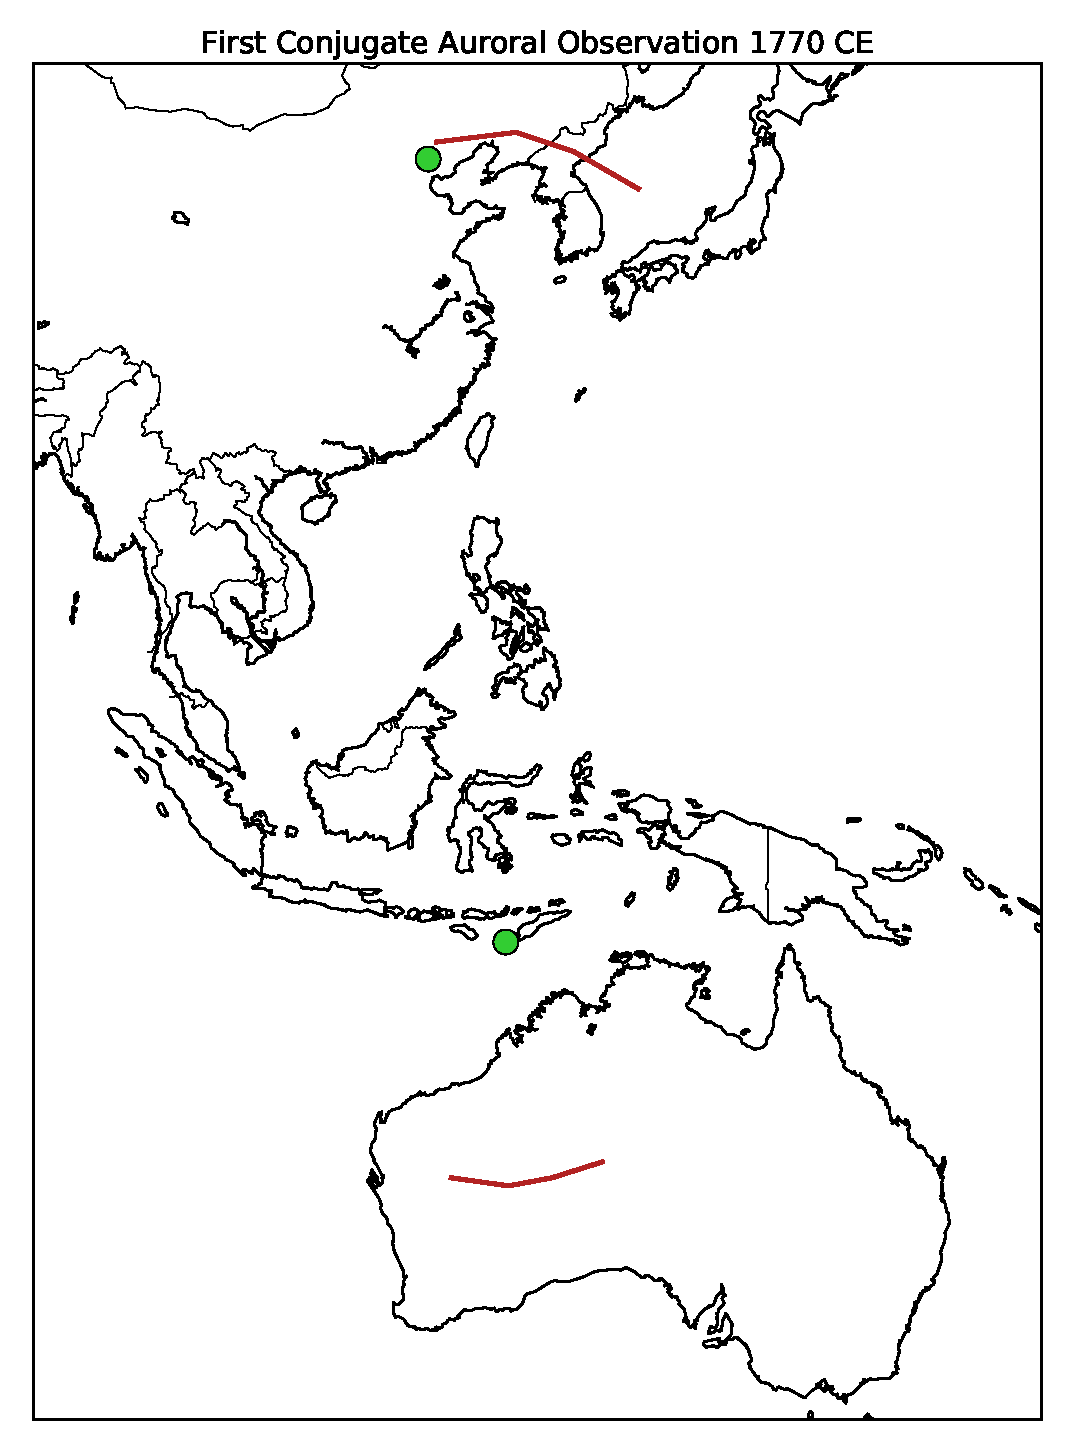
\includegraphics[width=0.8\linewidth]{gfx/firstconj}
    \caption{First recorded simultaneous auroral conjugate observation: September 16, 1770. Green circles represent observer locations. Red arcs indicate modeled location of \unit[630]{nm} forbidden [OI]21 auroral emissions \citep{willis1996}.}\label{fig:firstconj}
\end{figure}
The oldest observations record primarily red emissions more common at mid-latitudes driven by powerful solar storms greatly expanding the auroral oval over populated areas \citep{silverman1998}.

Nineteenth century auroral research included estimates of the height and shape of the aurora \citep{omholtbook}, which researchers in the twentieth century would recognize as proxies for the magnetospheric mechanisms driving the aurora.
Detailed records from South Asia and East Asia during and after the 1859 Carrington Event \citep{hayakawa2016east,keika2015caused} have allowed scientific speculation on what might be observed with contemporary instruments.
The pair of late nineteenth century auroral sketches in Figure~\ref{fig:chernouss6} \citep{chernouss2005} show an example of the opportunity and difficulty in extracting science quantities from ground observations of aurora due to perspective effects of the optically thin aurora.
That is, the observed brightness of aurora is equal to the line integral along the line of sight--stars are plainly seen through the aurora.
\begin{figure}\centering
    \begin{subfigure}[t]{0.45\linewidth}\centering
        \includegraphics[width=\linewidth]{gfx/chernouss6a}
        \caption{Auroral arc sketched from below.}\label{fig:1a}		
    \end{subfigure}
    \begin{subfigure}[t]{0.45\linewidth}\centering
        \includegraphics[width=\linewidth]{gfx/chernouss6b}
        \caption{Auroral arc sketched from oblique perspective.}\label{fig:1b}		
    \end{subfigure}
    \caption{Nineteenth century scientific auroral sketch by J. Sýkora \citep{chernouss2005}. 
    	In a typical case, two simultaneous observers, one beneath the arc would sees panel (a) and another observer $\sim \unit[100]{km}$ away sees panel (b).}
    \label{fig:chernouss6}
\end{figure}
Descriptions of aurora as rayed, striped, curtained, \&c. extend from the seventeenth century through the present.
Such terms are strongly biased by observer location, as lateral displacement of several kilometers can yield a rather different description of the same auroral form as discussed in \citet{semeter2012} and as modeled in Figure~\ref{fig:camres}.
Attempts to establish auroral heights presented great difficulty through the mid-1800s, with auroral altitude estimates spanning \unit[7..1100]{km} \citep{schwickert1833}.
Advances of the telegraph allowed distant synchronized photographs to be taken, and star registration techniques in part proposed by \citet{schwickert1833} were finally implemented by \citet{stormer1930} allowing plausible estimates of auroral height.

This dissertation describes the latest advances in joint studies of Langmuir turbulence associated with structured aurora using Incoherent Scatter Radar (ISR) and a network of synchronized cameras.
A schematic diagram \citep{schunk2006} of ionospheric features relevant to this dissertation is given in Figure~\ref{fig:aeroiono}.
\begin{figure}\centering
    \includegraphics[width=0.5\linewidth,trim=0 0 340 50,clip]{gfx/aeroiono}
    \caption{Ionospheric layers (from \citet{schunk2006})}\label{fig:aeroiono}
\end{figure}
The D-layer of the ionosphere lies from about 60..\unit[90]{km} and is a daytime only phenomenon due to intense short-wavelength UV bombardment from the sun, with the electron density enhancement quickly disappearing after sunset.
The E-layer of the ionosphere lies from approximately 90..\unit[150]{km} and is the altitude region where most finely structured aurora exists.
The F-layer of the ionosphere extends from \unit[150]{km} to several hundred km altitude. 
This dissertation discusses each of these elements in context and their connection to next generation instruments already being built.

\section{History of Scientific Auroral Observations}\label{sec:historyaurora}

Targeted observational efforts dedicated to aurora extended throughout the eighteenth and nineteenth centuries, noting several distinct colors and morphologies of various auroral forms \citep{wilcke1778,schwickert1833}.
Quantitative observations of auroral spectra required moving beyond Newton's seventeenth century prism experiments to get sufficient sensitivity and selectivity.
Eighteenth century prism and thermometer experiments \citep{herschel1800} were adequate to reveal the large infrared component of the solar spectrum, but were far too insensitive for quantitatively measuring spectra of non-solar features in the sky.
Rapid iteration by several researchers from about 1800--1850 opened the path for \AA ngstrom's founding role in scientific spectroscopy of quantitative solar observations \citep{reifacherman2014}.
Following the \citet{angstrom1869} reported measurement of \unit[557.7]{nm}, spectral measurements by \citet{fritz1881} recorded several emission lines, but with substantial wavelength error versus the much higher fidelity methods employed in 1899-1900 \citep{sykora1901,chernouss2005}.
The correct identification of atomic oxygen O responsible for the yellow-green \unit[557.7]{nm} line typically brightest at auroral latitudes (60..70$^\circ$ N) did not occur until 1923 \citep{chernouss2008}.

Instrumentation developed and distributed by \citet{rayleigh1924} established the global ubiquity of airglow and its distinction from aurora via carefully calibrated three-broadband filter arrangements.
Quantitative analysis of auroral intensity versus wavelength was accelerated in the latter half of the twentieth century \citep{seaton1954} as equipment improved and the theory rapidly evolved via increased observational efforts.
Theoretical predictions by \citet{garstang1951} for long-lived metastable [OI]32 \unit[557.7]{nm} lifetime $\sim \unit[0.7]{s}$ were observationally confirmed by \citet{omholt1955} using the apparatus of Figure~\ref{fig:omholtpmt}.
\begin{figure}\centering
    \includegraphics[width=0.6\linewidth]{gfx/omholtpmt}
    \caption{\citet{omholt1955} apparatus for \unit[23]{Hz} measurements in Tromsø during autumn 1954 of prompt \unit[427.8]{nm} emissions compared with forbidden long-lifetime \unit[557.7]{nm} emissions using a PMT to CRT and recorded on film strip.}\label{fig:omholtpmt}
\end{figure}
Stable auroral red (SAR) \unit[630.0]{nm} aurora with an absence of the \unit[557.7]{nm} emission common to polar aurora and airglow was discovered in 1956 with more sensitive imaging techniques \citep{baumgardner2007}.
Theoretical \unit[630.0]{nm} lifetime was likewise measured \citep{stoffregen1960} to be $\sim \unit[110]{s}$ via auroral spectrograph, since this lifetime would be exceedingly difficult to measure in an anthropogenic laboratory.
Extensive spectral work in the 1960s \citep{broadfoot1968} revealed high resolution relative intensities and corresponding chemistry of emissions that Rayleigh and associates broke into three coarse visible bands.
As aeronomical efforts expanded, the spectrum \citep{rees1974} and morphology of aurora were quantitatively and repeatably measured throughout the latter twentieth century \citep{nagy2015}.
Continued advances in spectroscopy led to fine quantification of auroral emission bands.
Laboratory verification of the lifetimes and other characteristics of kinetic reactions driving the optical emissions was enabled by instruments \citep{barrett1976} like that shown in Figure~\ref{fig:BellJar}.
\begin{figure}\centering
    \includegraphics[width=0.5\textwidth]{gfx/BarrettHaysBellJar}
    \caption{Electron penetration depth measurement mechanism used by \citet{barrett1976}}\label{fig:BellJar}
\end{figure}

\subsection{Twenty-first Century Auroral Observation}

As the twenty-first century dawned, auroral tomography first focused on reconstructing VER \citep{bjorn1998} $\sim \unit[1]{Hz}$ in concert with wide-angle camera networks \citep{donovan2006}.
As personal computing power underwent explosive growth, desktop 1-D ionospheric particle precipitation dynamics models \citep{blelly1996a} began to enable tying together ISR and optical observations across a wide range of wavelengths \citep{zettdis,dahlgren2013}.
Automated networked observatories have become the new way forward in geoscience and particularly in geospace.
This dissertation describes instruments developed to enable the cutting edge of ionospheric plasma science.


\subsection{History of Auroral Radio Science and Radar}\label{sec:historyisr}
As scientists scrambled to explain Marconi's improbable December 12, 1901 \citep{ratcliffe1974,belrose2001} \unit[3500]{km} transatlantic communications demonstration, early nineteenth century hypotheses and theory \citep{gauss1839} on the ionosphere were revived.
\citet{appleton1925} via careful observation iterated ionospheric theory and proved the bending of electromagnetic waves in the ionosphere.
Citizen scientists, radio amateurs, business and military users have benefited from thoughtful exploitation of frequency-dependent ionospheric refraction.

Tactical rockets freed by the end of World War II were pressed into service for geospace science almost immediately thereafter \citep{schmerling1966}.
The International Geophysical Year (IGY) of 1957-1958 opened orbital space to humanity, first with two Sputnik launches by the USSR.
The third anthropogenic satellite named Explorer 1 provided key information confirming the nature of the radiation belts persistence around Earth.
Before the availability of ISR and other specialized radars to study many simultaneous ionospheric plasma parameters, innovative closely spaced networks of receivers used radio stars and tailored transmissions to uncover apparent auroral $B_\perp$ velocities up to an order of magnitude faster than bulk plasma motion \citep{briggs1954}.
Bill Gordon's seminal monograph \citep{gordon1958} on incoherent scatter radar (ISR) theory led to several large ISRs being constructed within a decade.

Current ISR technology includes ``dish'' antennas such as at Arecibo, Millstone Hill and Søndrestrøm as well as several phased array radars including Jicamarca \citep{hysell2013jica}, EISCAT and AMISR.
Cubesats have been used to form a bistatic radar receiver for ISR, sensing \unit[0.1..1]{m} scale $B$-field aligned irregularities that PFISR is unable to resolve in monostatic mode \citep{bahcivan2014,cutler2013rax}.
Better spatiotemporal phased-array ISR methods have been modeled and simulated to better use scarce ISR resources.
For example, optimizing ISR beam pattern in the vicinity of a satellite while maintaining the overall observation pattern during a LEO pass \citep{swobodathesis}.
Networks of HF radars around each pole \citep{chisham2007} and growing ISR coverage fused with other sensors such as Cubesats and GPS TEC networks \citep{semeter2016} unlock increasingly fine spatiotemporal scales via synchronized simultaneous observation and inversion.

\section{Purpose}
The primary science purpose of the dissertation research is to use meticulous and systematic observational evidence to clarify the physical connections between Alfvénic auroral morphologies and ionospheric turbulence that produces coherent ISR backscatter.
The dissertation work resulted in a multi-station synchronized observatory recording auroral video at \unit[20]{ms} cadence.
As described in section~\ref{sec:fuspfisr} and chapter~\ref{chapter:sim}, this cadence is adequate for detecting and characterizing the associations between Langmuir turbulence and Alfvénic aurora.

Plasma traveling throughout the solar system and bound to planetary bodies is constantly subjected to changing magnetic field configurations and bulk flows.
A streaming instability results when a locally strong flow of particles (current), such as electronic precipitation into the ionosphere, causes longitudinal waves in the background plasma. 
Under frequently occurring conditions, the plasma wave grows exponentially into a streaming instability.
The ionospheric turbulence creates signatures readily detected by sufficiently fast sampling ISR and synchronized camera systems, allowing distinction between various types of Alfvén wave-sourced perturbations and characterization based on remote sensing inversion algorithms as developed in chapters~\ref{chapter:sim} and \ref{chapter:fusion}.

Each important aspect of the sensing system design and implementation is described to allow reproduction of the experimental apparatus and build confidence in the character of its output products.
Section~\ref{sec:aurorabasic} introduces key facets of optical auroral observation and processing advanced by the dissertation, expanded upon in chapter~\ref{chapter:inst}.
Section~\ref{sec:isrbasic} introduces connections between ISR and HiST optical observations and inversion, expanded upon in chapter~\ref{chapter:fusion}.
The necessary algorithms created to detect Alfvénic aurora and ion-acoustic turbulence seen in radar are introduced in section~\ref{sec:intdiscrim} and described in chapter~\ref{chapter:discrim} with additional applications showing the generality of the technique in appendices~\ref{chapter:marsis} and \ref{chapter:passive}.

\FloatBarrier
\subsection{Characterizing sources of fine-scale auroral structure}\label{sec:aurorabasic}
The optically thin aurora with observed optical intensity $\mathscr{I}$ due to auroral volume emission rate (VER) $p$ looking along direction $\vect{r}$ is described by
\begin{equation}\label{eq:bint}
\mathscr{I} = \int_0^\infty p(\vect{r})\textrm{d}\vect{r}
\end{equation}
implying that ground-observed auroral brightness strongly depends upon viewing angle.
Additional important factors such as wavelength-dependent atmospheric absorption between the aurora and observer are detailed in chapter~\ref{chapter:sim}.
Non-uniqueness of the observational system is implicit in (\ref{eq:bint}) as demonstrated with the examples in Figure~\ref{fig:bint} for an optically thin 2-D phantom. 
\begin{figure}\centering
    \begin{subfigure}[t]{0.45\linewidth}\centering
        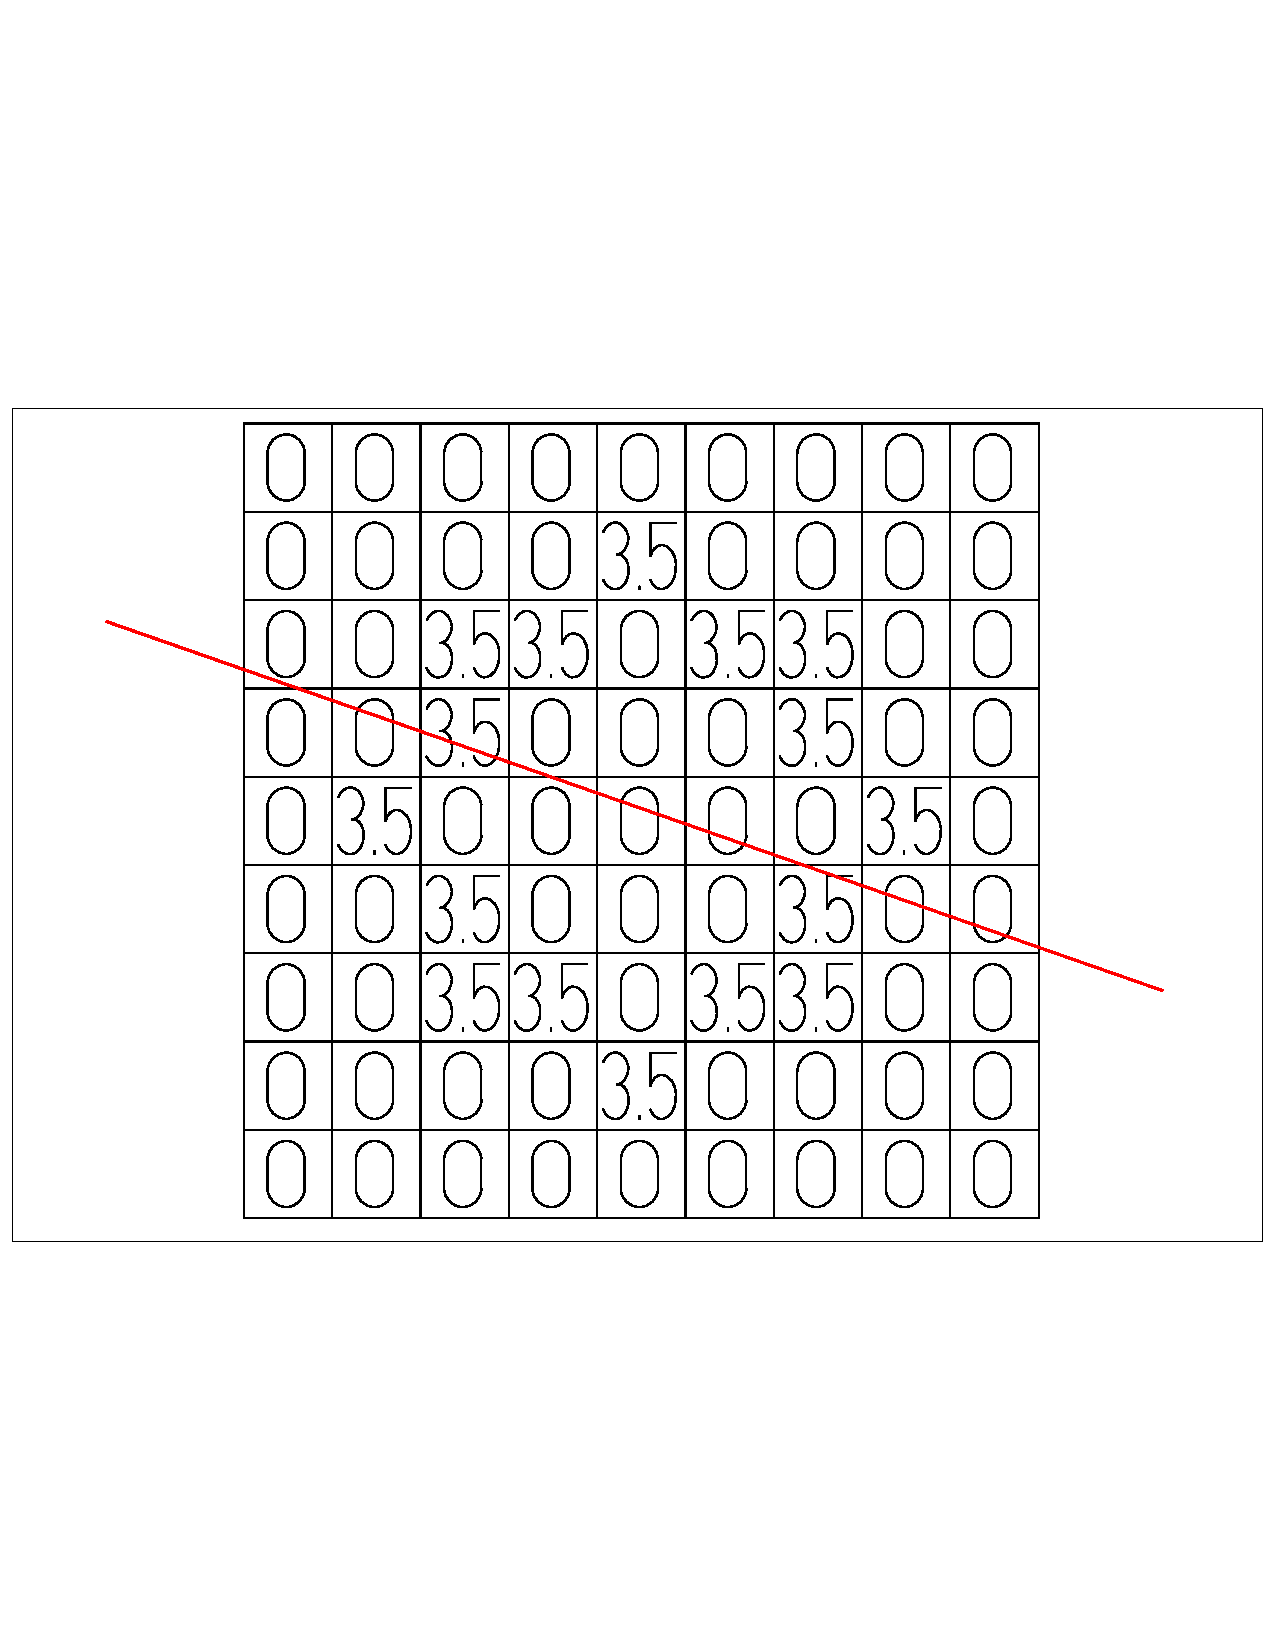
\includegraphics[width=\linewidth,trim=50 200 50 200,clip]{gfx/circle}
        \caption{Hollow optically thin structure with line-of-sight.}		
    \end{subfigure}
    \begin{subfigure}[t]{0.45\linewidth}\centering
        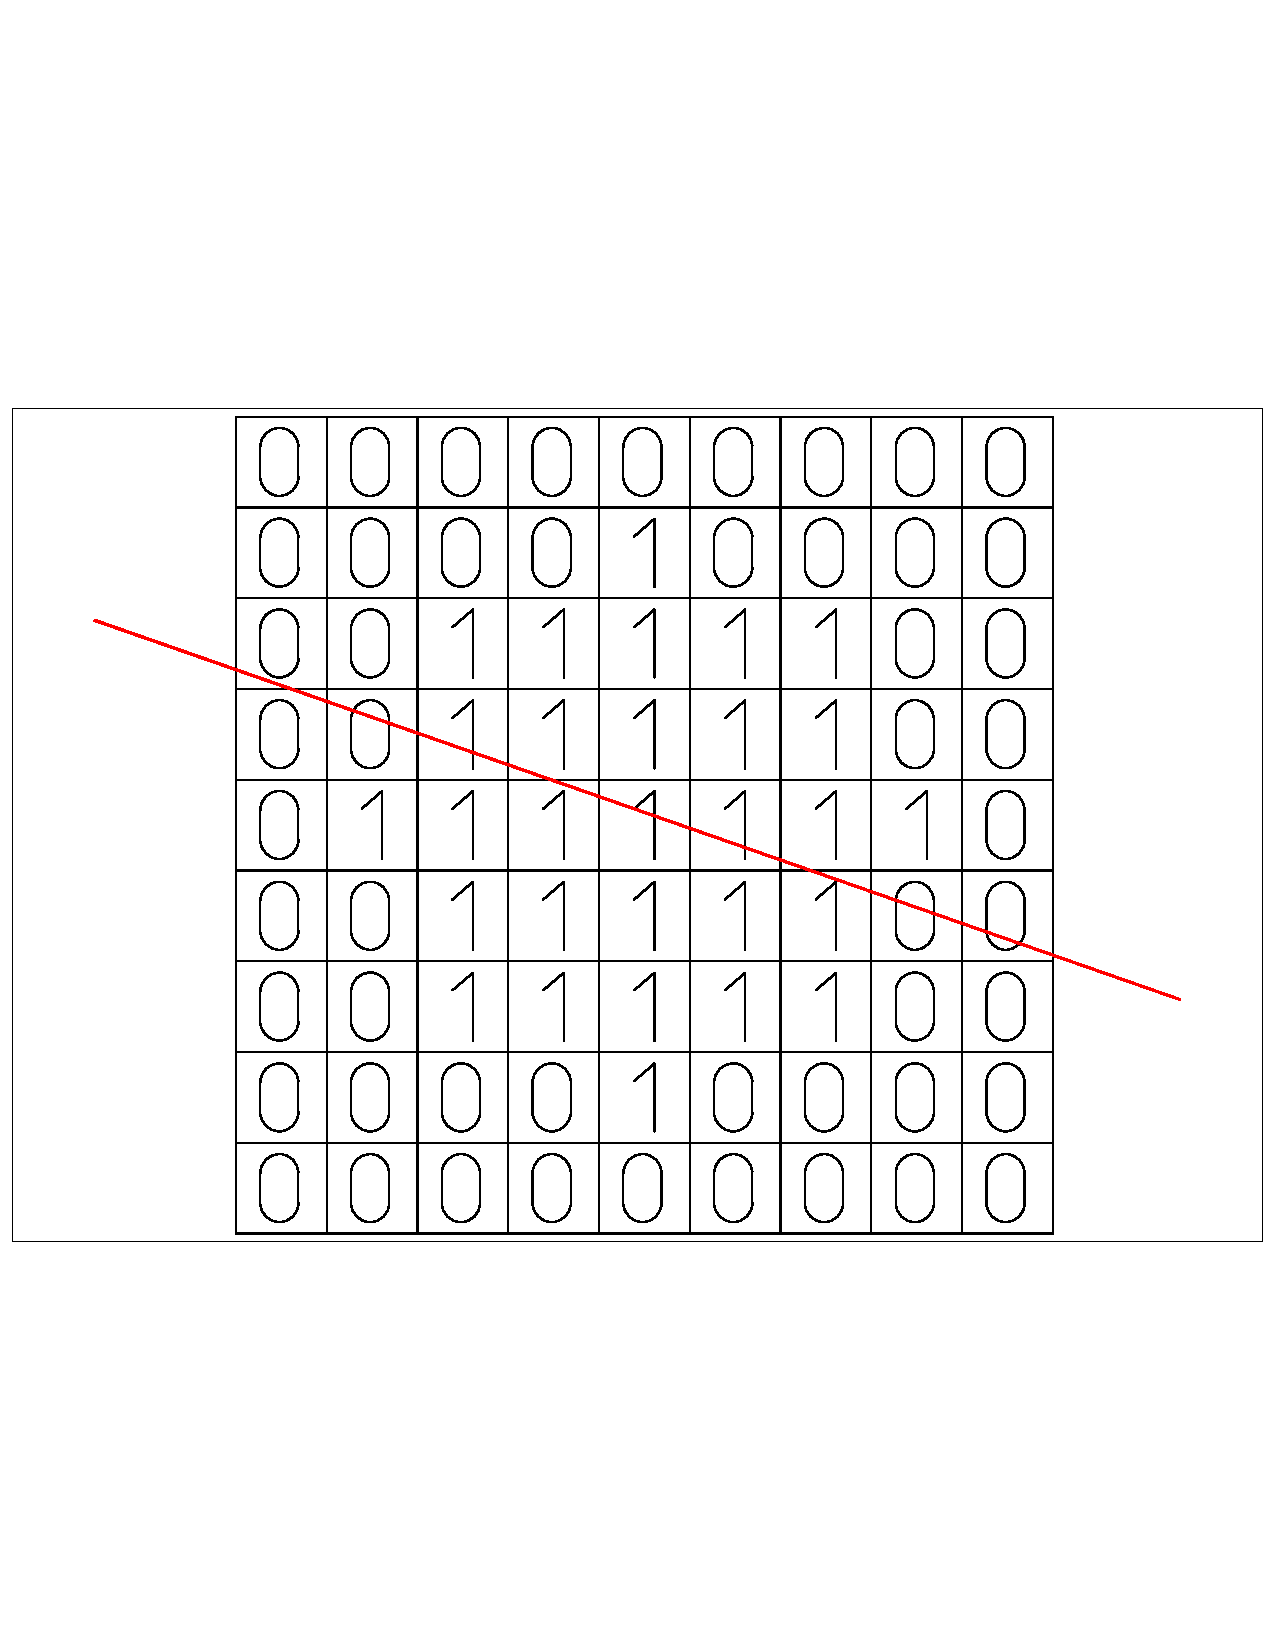
\includegraphics[width=\linewidth,trim=50 200 50 200,clip]{gfx/disk}
        \caption{Filled optically thin structure with line-of-sight.}		
    \end{subfigure}
    \caption{Optically thin phantoms with red line-of-sight integral. Completely distinct forms after line-integration give the same result, an example of the non-uniqueness problems inherent to auroral remote sensing.}\label{fig:bint}
\end{figure}
Whether the observed target is disk, circle, spline or other arbitrary form, line integration of distinct forms can lead to the same integrated (observed) result.

We assume the auroral cameras are boresight-aimed at magnetic zenith. 
Non-uniqueness becomes increasingly important for large camera viewing angle from magnetic zenith $\theta \gg \unit[1]{degree}$.
As camera ground spacing increases beyond $x \sim \unit[10]{km}$ increasingly poor resolution of fine detail along $B_\perp$ results as demonstrated in Figure~\ref{fig:camres}.
\begin{figure}
	\begin{subfigure}[t]{0.45\linewidth}\centering
		\includegraphics[width=\columnwidth]{../gfx/L3cam}
		\caption{Viewing geometry for auroral arc with cameras at $x \in (0,3,10)$~km.}
	\end{subfigure}
	\begin{subfigure}[t]{0.45\linewidth}\centering
		\includegraphics[width=\columnwidth]{../gfx/I3cam}
		\caption{Intensity $I$ for three cameras.}
	\end{subfigure}
	\caption{Notice how the intensity of the green line for $x=\unit[10]{km}$ has smeared out the \unit[1.5]{km} spaced arcs, demonstrating a non-uniqueness issue.}
	\label{fig:camres}
\end{figure}
Figure~\ref{fig:camres}(b) shows the non-uniqueness issue in auroral tomography, particularly for cameras widely spaced from the auroral arc of interest.
Alfvénic splitting auroral arcs with widths in the \unit[0.01..1]{km} range are best observed with cameras spacing $x < \unit[10]{km}$.

The diverse colors and shapes of the aurora have been the focus of human study and speculation for centuries.
The colors of the aurora consist of isolated spectral lines, close groups of spectral lines and continua of spectral bands.
Auroral optical emissions are photons released as excited particles (atoms and molecules, ions and neutrals) relax and emit a photon with wavelengths determined by quantum physics.
The precipitating electron energy at the top of the ionosphere likewise varies between monoenergetic, a band-limited uniform spectrum or a complex spectrum having one or more peaks in a broadband differential number flux spectrum.
% NOTE: example figure here?
Precipitating particle sources include electrons mirroring in the upper ionosphere, particles ejected from the plasma sheet or launched from the magnetotail.
More important to this work than where the electron came from is what acceleration process the particle experienced before crashing into the ionosphere.
Alfvén wave accelerated particles have key signatures in the differential number flux spectrum.
Alfvén wave accelerated electrons kinetically reacting with E- and F-region ionospheric particles give particular signatures in high-speed auroral and ISR observations that are connected observationally in this dissertation.
These factors imply that an appropriate inversion algorithm may yield new science conclusions about the association and characteristics of Alfvénic aurora and plasma turbulence.

Essential to the analyses in this dissertation is the fact that auroral behavior in the $B_\parallel$ dimension may be modeled by numerical solutions to partial differential equations describing energy deposition along a flux tube.
The important \textit{a priori} inputs to such models include solar zenith angle (SZA) (that is, angle of the sun from local zenith).
SZA is commonly used in auroral studies because of the inherent angular ambiguity near the horizon due to refraction. 
When the sun is seen to be at the horizon, the sun is already geometrically below the horizon under typical conditions.
During the day, photodissociation due to solar EUV gives rise to the D-layer ionosphere, absorbing MF.
During solar energetic particle events lower HF wavelengths are also absorbed.

Neutral atoms and molecules along with ions are a prerequisite for structured aurora.
These ionospheric particles are impacted by electrons in finely structured (in $B_\perp$) beams to create structured aurora.
Just before Sputnik I was launched, \citet{chamberlain1957} raised the possibility that locally-accelerated electrons were responsible for fine auroral structure in the E-region, while prior work such as \citet{seaton1954} suggested electrons could not generate E-region aurora.
The first group of Sputnik and Explorer spacecraft in 1957--1958 made structured proton aurora in the E-region seem unlikely and a local acceleration mechanisms for electrons probable \citep{krassovsky1959,wallace1959}.
The primary role of the electron in structured E-region aurora was solidly established by 1960 with \textit{in situ} sounding rocket sensors of increasing fidelity revealing typical scales and dynamics of auroral precipitation.
Of note are the pair of \unit[120]{km} apogee sounding rockets \citep{mcilwain1960} determining the important result that proton particle flux was $\ll 1\%$ electron particle flux, electron energy flux was at least 10 times that of proton energy flux, and small amounts of differential number flux were found.
1963 satellite measurements \citep{sharp1965} at $\unit[8]{ms} \Leftrightarrow \unit[63]{m}$ sampling cadence showed rapidly changing energy spectrum amidst a more slowly changing energy flux.
These observations confirmed that most of the auroral flux had particles less than \unit[10]{keV} with the largest differential number flux at energies $\ll \unit[1]{keV}$.

\subsubsection{Objectives related to characterizing sources of fine-scale auroral structure}
\citet{chaston2007how} noted the characteristics of Alfvénic aurora consistent with the design of the HiST system \citep{hirsch2016}.
The following HiST performance metrics were vital to success:
\begin{enumerate}
	\item Observe aurora with cadence $\leq\unit[20]{ms}$
	\item Operate unattended to catch few seconds of good data from weeks of observation
	\item Time sync between sites $\ll \unit[1]{ms}$ and absolute time sync $\ll\unit[1]{ms}$ for data fusion with other instruments
	\item Physics-based forward model to allow capture of broadband filtered light, enabling fast imaging with comprehensive representation of auroral kinetic reactions in the data inversion process
\end{enumerate}
These metrics were met and exceeded in performance as developed throughout the dissertation.

\FloatBarrier
\subsection{Joint ISR-Optical Analysis}\label{sec:isrbasic}
Phased-array incoherent scatter radars enable sampling of arbitrarily arranged beam patterns, sampled with nearly instantaneous switching between beam angular position.
PFISR has thus been used for a wide variety of auroral and ionospheric studies, given its location under the auroral oval and within reach of the southern boundary of northern polar cap activity.
The model-based iterative reconstruction (MBIR) from the HiST system has infrequent opportunities for independent confirmation from on-orbit sensors during the sub-second events of interest.
Even with an \textit{in situ} sensor available in the form of a rocket or satellite in just the right place during a sub-second event, the space-time ambiguity of any \textit{in situ} sensor attempting to measure a highly spatiotemporally dynamic event is unacceptably large.

The purpose of siting an instrument such as HiST near PFISR is about more than confirmation--the ionization production by the intense spray of magnetospheric electrons into the ionosphere creates plasma density gradients.
These gradients themselves create measurable radar backscatter, and when instabilities grow, the backscatter can grow to 1000 or more times greater strength than the quiescent conditions just tens of milliseconds before.
By estimating the precipitation characteristics above the ionosphere where kinetic interaction are minuscule compared to inside the ionosphere, the turbulence measured by the radar can be directly connected to its source.
The fine scale structure and growth of plasma instabilities on these spatiotemporal scales have been simulated \citep{akbari2015}, but confirmation of these models comes about through detailed measurements of the natural laboratory provided by Earth, HiST and PFISR as performed in chapter~\ref{chapter:fusion}.

\subsubsection{Objectives related to joint ISR-Optical Analysis}
The objectives of this dissertation with regard to joint ISR-Optical analysis are mainly accomplished via MBIR. 
MBIR on HiST high-speed synchronized video streams reveals the spatiotemporal structure of precipitation driving streaming instabilities and strong Langmuir turbulence.
Zakharov simulations \citep{akbari2015,zakharov1d} reveal the nature of instabilities developed from strong lower energy precipitation and their modeled ISR spectrum.
HiST provides high time resolution estimates of that spectrum, allowing fine scale plasma turbulence model validation.

\FloatBarrier
\subsection{Discrimination of Ionospheric Turbulence in Radar and Optical Data}\label{sec:intdiscrim}
Detection of ionospheric turbulence in multiple sensor types is vital to proving a consistent connection between particular auroral manifestations and the turbulence seen in radar sensors.
Methods were developed using extensions of standard radar practice and novel applications of computer vision algorithms to the unusually low SNR presented by auroral video.
Standard computer vision techniques are applied to high SNR video, tracking rigid bodies in the face of occlusion, lighting variation and other such challenges.
Auroral video quite literally breaks many of these assumptions, and so a method for reliably detecting structured aurora is developed in chapter~\ref{chapter:discrim}.

Quantifying collective behavior of enormously large numbers of objects is an active area of research in computer vision.
The social force model \citep{mehran2009} assigns low-density particles to a high-density optical flow field to detect outlier behavior.
Mars rovers suffer far more extreme constraints on data bandwidth than HiST, additionally with a tiny fraction of the computing power, yet cloud and dust devil detection algorithms have been successfully implemented \citep{castano2008}.
Tracking of ``enormously large'' numbers of bats using three IR cameras has been accomplished to great quantitative effect \citep{betke2007,betke2008}.
None of these implementations faces quite the same issues as auroral researchers.

With awareness of prior efforts in quantifying fine structured auroral behavior \citep{semeter2006}, the approach in this dissertation to detecting fine structure aurora represents a break with known auroral computer vision applications.
The algorithm employed, while engaging several distinct computer vision techniques, is a discrimination step before invoking the far more computationally costly MBIR method.
Since the target characteristics are themselves noise, an algorithm built and implemented to detect collective behavior of noise is described in chapter \ref{chapter:discrim}.

\subsubsection{Objectives related to Discrimination of Ionospheric Turbulence in Radar and Optical Data}

The objective of implementing the computer vision algorithms is to avoid an impossibly large computational burden of running the full HiST inversion algorithm on all auroral video collected.
The alternative of manually examining all video is humanly infeasible, both due to time cost and levels of aurora too faint to be seen without literally watching the video stream with taking say every tenth frame to speed the process.


\section{Contributions}\label{sec:contrib}
The central focus of the dissertation is on applications of modern radar and optical remote sensing techniques to advance understanding of finely structured electron beams interacting with the ionosphere.
This involved constructing two networked auroral observatory systems deployed to Greenland (DMC) and central Alaska (HiST phase 1), and the design and build of HiST phase 2 for spring 2018 deployment in Alaska with dual cameras and TEC receivers.
As is typical in dissertation work, a large subset of the work resulted in publications and presentations.
Another substantial subset of the work resulted in contributions to state of the art geospace data processing and remote sensing data inversion software relevant to auroral, atmospheric, ionospheric and magnetospheric studies.
Contribution categories concomitant to the dissertation work include: scholarly, instrumental, software, and algorithmic.

\subsection{Novel Contributions}
The dissertation contributions leading directly to scholarly work are enumerated in this section.
\begin{enumerate}
       
    \item A joint analysis method for ISR and optical data, confirming and characterizing the relationship between Alfvénic aurora and ionospheric turbulence measured as strong ISR backscatter, described in \citet{hirsch2017jgr} and chapter~\ref{chapter:fusion} as well as \citep{hirsch2016unh,hirsch2016precip,hirsch15agu} 
    
    \item A novel auroral tomography data inversion algorithm using first principles physics model based iterative reconstruction, described in paper \citet{hirsch2016} and presentations/posters \citet{hirsch2015cedarposter,hirsch2015mtssp,hirsch2014agu,hirsch2014cedar,hirsch2014cedartalk,hirsch2014ursi,hirsch2012}
    
    \item A novel collective behavior discrimination algorithm useful for detecting structured aurora, making manageable the enormous amounts of data (terabytes per day) inherent in the observations necessary for \citep{hirsch2017jgr,hirsch2016} as detailed in chapter~\ref{chapter:discrim}, appendices~\ref{chapter:marsis} and~\ref{chapter:passive} and \citep{swoboda2016python,hirsch2016bigdata,hirsch2015cedartalk}
\end{enumerate}


\subsection{Instrumental Contributions}
The DMC and HiST systems represented substantial advances over prior auroral observation techniques, and were pressed into a variety of observational services.
\begin{enumerate}
	
	\item as distinguished from later work such as \citet{kataoka2016high} using longpass RG665 filters, HiST BG3 bandstop filters includes the critical N2+ emissions in the blue-UV range AND the deep red/near IR wavelengths that reveal the fastest ground-observable features in the aurora
	
	\item HiST cameras were a key part of a joint ISR-optical high-speed meteor triangulation and radar cross section (RCS) experiment to accurately estimate meteoroid mass \citep{limonta}
	
	\item HiST cameras provided prompt-emission only filtered video stream to complement unfiltered (metastable dominated) sCMOS for observation of IAW flickering aurora in February 2014 Polaris campaign at PFRR \citep{kataoka2015,fukuda2016}
	
	\item HiST cameras at \unit[20]{ms} cadence complemented \unit[13]{s} all-sky cameras for April 2014 PINOT mission at PFRR \citep{fallen2014,nishimura2014,makarevich2014}
	
	\item HiST cameras complementing additional narrowband-filtered EMCCD cameras, all-sky cameras, and other sensors for 3 March 2014 GREECE rocket flight, yielding \textit{in situ} sensing from \unit[300]{eV} to \unit[200]{keV} electrons, with \unit[2..200]{keV} measured at \unit[100]{ms} cadence \citep{michell2014agu,samara2014,grubbs2014,ogasawara2014,ogasawara2016,ogasawara2016a}
	
	\item HiST cameras provided high-speed video for use with the LiCHI hyperspectral imager, which provided four narrowband tunable wavelengths vs. HiST broadband prompt emissions at PFRR \citep{goenka2016,goenka2015,goenka2014}
	
	\item DMC camera pair provided insights into prompt-emission filtered aurora as seen simultaneously at decameter and kilometer scale at \unit[30]{fps}, while supporting high speed ISR measurements \citep{vierinen2016}
    
\end{enumerate}


\subsection{Algorithmic Contributions}
The algorithmic contributions of the dissertation work represent generalizable contributions that go beyond a specific software implementation, more than a set of techniques contrived to solve a particular problem.

\begin{enumerate}
    
   \item Contributing to the new high-speed plasma line receiver techniques in \citet{vierinen2016agu,vierinen2016,bhatt2016sondre}, developed the analysis package \citet{dmcutils} that examined the time lag between electron density enhancements measured with Søndrestrøm ISR versus prompt auroral emissions seen through the DMC BG3 filter
    
   \item Observing high energy precipitation with characteristic energy $E_0 \gg \unit[100]{keV}$ requires dedicated instrument design, as well as models \citep{glowaurora,gridaurora} designed for high energy precipitation yielding X-rays as short as \unit[20]{\AA}, as proposed in \citet{sivadas2016cedar}
  
\item the collective behavior computer vision algorithm developed in chapter~\ref{chapter:discrim} is useful for distinguishing structured aurora from diffuse aurora, stars, clouds, and other undesired targets.

\item A collective behavior computer vision algorithm was developed for passive FM hitchhiker radar, as detailed in chapter~\ref{chapter:passive}.

\item Absolute image time recovery algorithm exploiting camera FPGA hardware outputs accounts for glitches and other nonidealities rampant even in high-end scientific cameras, vital for fusing data from heterogeneous sensors as described in section~\ref{sec:hist}.

\item A physics model based iterative reconstruction algorithm (MBIR) incorporating broadband auroral emissions to estimate magnetospheric precipitation characteristics at the top of the ionosphere, as described in chapter~\ref{chapter:sim}.

\item Retrieval method and automatic detection of local plasma oscillations for MARSIS radar exploring the Martian ionosphere as described in chapter~\ref{chapter:marsis}. Code developed was mutually shared with a European researcher, and over the course of several Skype sessions, they had developed a dual to the author's methods \citep{andrews2013} to exploit the decade's worth of MARSIS data in discovering and quantifying stable regions in the Martian dayside ionosphere \citep{andrews2014} and their driving parameters \citep{dieval2015} especially by crustal fields \citep{andrews2015}, analyzing a highly anomalous high-altitude plume in the Martian ionosphere \citep{andrews2016}, exploring topside Martian ionospheric morphology during various solar wind conditions \citep{withers2016} and characterized precipitation outcomes \citep{dubinin2015}.

\end{enumerate}

\subsection{Software Contributions}
Software collaborative contributions during the dissertation work include:

\begin{enumerate}    
    \item Update auroral tomography software suite \texttt{AIDA-tools} \citep{aidatools} to run on modern MATLAB versions
    
    \item Reimplement LOWTRAN atmospheric absorption model in Python \citep{lowtran} replacing 1980s Fortran mainframe/punched interface \citep{lowtran7} with easy to use \texttt{f2py} Python-Fortran interface
    
    \item Auroral phantom generator \citep{cvphantom}, incorporating several canonical auroral types including discrete arcs, vortex streets and vortex streets--including arbitrary motion (direction, speed) vs. time
    
    \item Geospace coördinate conversion suite for Python, vectorized to allow fast, accurate conversion between coördinate systems \citep{pymap3d}
    
    \item Highly efficient RINEX reader for Mahali GPS \citep{pankratius2014,semeter2016,pankratius2016ams} allowing reading large numbers of files from the Mahali distributed GPS network, forming a basis of the Geoscience Ionospheric Toolkit (GSIT) \citep{gsit}.
    
    \item Update seven optical flow estimation programs \citep{barron1994code} from \citep{barron1994} to compile on modern Intel PC/Mac for use with \citep{cviono} in discriminating auroral forms.
    
    \item enhanced 1-D Zakharov simulations \citep{zakharov1d} used in \citep{akbari2015,akbari2016,akbaridis} to run in parallel with command-line specified parameters
    
    \item Created numerous geospace data reading and formatting packages for instruments including DASC \citep{dascutils}, P-DMSP \citep{meridianreader} and multiple AMISR locations plus Søndrestrøm \citep{isrutils}
    
    \item contributed core code segments to GeoData and several associated programs \citep{geodata} used in \citet{swoboda2015,swobodathesis}
    
    \item Created reader and plotter for THEMIS ASI GBO \citep{donovan2006} data \citep{hirschthemis}
\end{enumerate} 

    
\cleardoublepage

% !TEX root = thesis.tex

\chapter{Background}
\label{chapter:physics}
\thispagestyle{myheadings}

\graphicspath{{Physics/}}

\epigraph{If each energy quantum of the exciting light, independent of all others, emits its energy to electrons, the velocity distribution of the electrons will be independent of the intensity of the excitation light. On the other hand, the number of electrons leaving the body will be proportional to the intensity of the excitation light under otherwise similar circumstances.... It must therefore be assumed that the kinetic energy of an electron is used to generate many light energy quanta.}{\citet{einstein1905}}

The fine spatiotemporal dynamics of structured aurora have been studied for over a century, kicked off by leaders including Birkeland and Størmer from the 1890s onward.
Geoscientists by the time of \citet{birkeland1908} understood that particles flowing from the sun interacted with the geomagnetic field.
Before 1910 it was understood that perturbations of the geomagnetic field were directly related to the currents carried by what \citet{mcilwain1960} confirmed \textit{in situ} to be electrons for finely structured aurora.
A common metric for finely structured aurora is that aurora of width along $B_\perp$ one kilometer or less, which is associated with precipitating electrons.
The narrowest auroral structures driven by protons are nearly two orders of magnitude greater in width--interesting in their own right, but outside the scope of what the present HiST system is designed to observe.
Inverted-V and Alfvénic aurora are two well-known types of finely structured aurora with distinct electron acceleration mechanisms distinguishable by \textit{in situ}, radar and optical sensors.
Additional theories on fine structured auroral generation mechanisms include:
\begin{enumerate}
    \item Striped auroral patterns in diffuse background: whistler-mode upper band chorus \citep{nishiyama2012,sergienko2008}  
    \item ``smokelike'' aurora: consisting of multiple thin wispy legs of approximately \unit[1..5]{km} width \citep{ebihara2010}, thought to be an interchange instability between hot electrons disturbing cold plasma
\end{enumerate} 
While we have not specifically examined the latter two cases due to their relative rarity versus Alfvénic aurora, their characteristics are within the observational capabilities of the HiST system.

Geospace numerical modeling covers scales from particle-in-cell (PIC) simulations involving millions to billions of particles \citep{young2016} to the solar wind throughout the solar system \citep{echim2011}.
The lifecycle dynamics of a geomagnetic storm are modeled from the inner magnetosphere \citep{tsyganenko2005} out to the solar wind interface \citep{tsyganenko1996}.
While this dissertation focuses on the electron lifecycle in the ionosphere, sufficient understanding of the magnetosphere is a prerequisite for geospace study.
The \citet{johnson1960} model expressed in Figure~\ref{fig:1960mag} was rapidly improved upon in the next several years \citep{mead1964} with the benefit of an increasing number of \textit{in situ} measurements driving iteration of improved models and theories.
\begin{figure}
	\includegraphics[width=\linewidth]{gfx/1960mag}
	\caption{\citet{johnson1960} magnetospheric model, without benefit of \textit{in situ} measurements.}\label{fig:1960mag}
\end{figure}
In Figure~\ref{fig:1960mag}, the sun is far off the left side of the page.
In the absence of the roughly \unit[400]{km/s} solar wind, the nearly dipolar geomagnetic field would appear roughly symmetric about the magnetic equator and rotationally symmetric across all longitudes.

The solar wind compresses the dayside magnetic field, and drags out the magnetotail to tens of $R_E$.
Every several hours, a substorm occurs where the magnetotail to the right of Figure~\ref{fig:1960mag} becomes overloaded with plasma, a plasmoid detaches permanently, and the magnetotail settles in closer to Earth.
This cycle repeats endlessly, but with widely varying intensity of waves, particles, and ultimately precipitation incident into the ionosphere as represented in Figure~\ref{fig:magcirc}.
\begin{figure}\centering
	\includegraphics[width=\linewidth,trim=50 370 150 40,clip]{gfx/magcirc}
	\caption{Simplified model for two mechanisms responsible for structured aurora. 
		The parallel potential lines represent double-layers leading to inverted-V aurora. 
		The sinusoid represents IAW acceleration. 
		The contours represent $B$.}
	\label{fig:magcirc}
\end{figure}
Conservation laws dictate that the gradients involved in geomagnetic system reconfiguration must be felt throughout the geomagnetic system.
The magnetic field lines act as invisible transmission lines where ions and electrons travel freely, mirroring between the lower magnetosphere and magnetotail.
Particles that gain sufficient energy, whether via acceleration processes or other events are at risk of being lost into the ionosphere through stochastically predictable, TRANSCAR modeled energy deposition processes.
%The cold return current comes back up $B$ into the magnetosphere, closing the circuit depicted in Figure~\ref{fig:migcircuit}.
%\begin{figure}
%	\includegraphics[width=\columnwidth]{gfx/migcircuit}
%	\caption{Alfven-wave transmission of magnetosphere-ionopshere-ground coupling, from \citet{kikuchi2014}.}
%	\label{fig:migcircuit}
%\end{figure}
%\citet{kikuchi2014} further developed the circuit element model to compute characteristic impedance and reflection coefficients of the Alfvénic transmission line model and the waveguide model coupling ionosphere to ground.
%%\begin{figure}
%	\includegraphics[width=\linewidth]{../gfx/mi-transmission-line}
%	\caption{\citet{kikuchi2014} circuit element model to compute reflection coefficients for the Alfvenic M-I coupling interface and waveguide model for G-I coupling.}
%	\label{fig:distcirc}
%\end{figure}

These lost particles do not go quietly, rather their ``death'' is transmitted via electromagnetic waves from ELF through HF \citep{labelle2002}, as well as heat, light and X-rays \citep{raymont2008}.
Strictly speaking the particles are not lost, but they may join the cold plasma background, participate with the currents in the auroral electrojet and/or once again rejoin the current systems in the magnetosphere \citep{hargreavesbook}.
Although the understanding of auroral generation mechanisms are still incomplete at Earth and other planetary bodies, searches for radio \citep{nichols2012} and UV \citep{france2010} emissions from exoplanets have been undertaken.
Exoplanet auroral measurements help constrain the atmospheric morphologies and compositions.
Some of the challenges of quantifying auroral radio emissions in the tens of MHz range have been complicated by possibly interfering radio emissions from the magnetosphere of Jupiter \citep{labelle2002}, so more careful study is needed.
The many types of emissions emanating throughout the auroral lifecycle would consume volumes to describe, thus this chapter covers the topics necessary for elucidating the remainder of the dissertation.

This dissertation presents new ground-based observational capabilities associating ionospheric plasma flows and turbulence with Alfvén wave accelerated electron precipitation.
In this chapter physical context is provided for discussion in the following chapters concerning characterization of ionospheric turbulence associated with Alfvénic aurora.
One of the fundamental behaviors influencing the scale of aurora seen, and distinguishing between the behavior of electron aurora versus proton aurora is the gyration of charged particles in the presence of a magnetic field.
We therefore begin the physics background with single particle motion and describe the acceleration of these particles by Alfvén waves.
The energy deposition and production of auroral light emissions rounds out this chapter.

\section{Planetary Plasma}
Plasma about planetary bodies are infused with magnetic fields. 
For those planetary bodies without intrinsic magnetic fields, crustal magnetic fields such as at Mars and induced magnetic fields caused by the magnetic field lines draping around the planetary body nonetheless are essential to describing particle behavior.
Comets also experience an induced magnetosphere, as confirmed by \textit{in situ} measurements \citep{israelevich1994}.
Although diagrams of the geomagnetic system lend themselves to complexity, the basic particle behavior can be described starting with Newton's Second Law of Motion.


\FloatBarrier
\subsection{Single Particle Motion}
The basic equation of motion for a mass $m$ experiencing a force $\vect{F}$ is
\begin{equation}\label{eq:Feqma}
\vect{F}=m\vect{a} = m \frac{d\vect{v}}{dt}.
%\marginnote{eqn. of motion}
\end{equation}
In the presence of electric field $\vect{E}$, the Lorentz force on a particle with charge $q$ is
\begin{equation}\label{eq:lorentzforceBeq0}
\vect{F} = q\vect{E}.
%\marginnote{Lorentz force, \ensuremath{B\equiv0}}
\end{equation}
In the presence of a magnetic field $\vect{B}$ and electric field $\vect{E}$, a particle at rest will be accelerated and gyrate about $\vect{B}$, driven by the Lorentz force
\begin{equation}\label{eq:lorentzforce}
\vect{F} = q\left(\vect{E} + \vect{v}\times\vect{B}\right).
%\marginnote{Lorentz force}
\end{equation}
The decomposition of \eqref{eq:lorentzforce} into components
\begin{equation}\label{eq:Fperppar}
\vect{F} = \vect{F}_\parallel + \vect{F}_\perp
\end{equation}
where $\vect{F}_\parallel\in \vect{F} \parallel \vect{B}$ and $\vect{F}_\perp \in \vect{F} \perp \vect{B}$\ leads  to the notion that charged particles will gyrate in a magnetic field, with motion along $\vect{B}$ driven by $\vect{E}$ \citep{cravensbook}. 

For simplicity we drop the vector symbol where the context is clear.
The sign of $q$ indicates that positive and negative particles will move in opposite direction for both $F_\parallel$ and $F_\perp$. 
Aurora is observed \citep{borovsky1993} from the solution of~\eqref{eq:Feqma} for particles along $B$
\begin{equation}\label{eq:vpar}
v_\parallel = v_{\parallel,0} + \frac{F_\parallel}{m}t
%\marginnote{\ensuremath{v \parallel B}}.
\end{equation}
The gyroradius
\begin{equation}\label{eq:gyrad}
r_L = \frac{m_s v_\perp}{qB}
%\marginnote{gyroradius}
\end{equation}
and gyrofrequency
\begin{equation}\label{eq:gyfreq}
\Omega_s = \frac{q B}{m_s}
%\marginnote{gyrofrequency}
\end{equation}
follow from solving for 
\begin{equation}\label{eq:vperp}
v_\perp^2 = v_x^2 + v_y^2 
%\marginnote{\ensuremath{v \perp B}}
\end{equation}
with components
\begin{align}
v_x &= v_\perp \cos{\left( \Omega t + \theta \right)} \label{eq:vxy} \\
v_y &= \mp v_\perp \sin{\left( \Omega t + \theta \right)} \nonumber.
\end{align}
The pitch angle
\begin{equation}\label{eq:pitch}
\alpha_p = \tan^{-1}{\frac{v_\perp}{v_\parallel}}
%\marginnote{pitch angle}
\end{equation}
of a particle is the angle between $\vect{v}$ and $\vect{B}$.
As discussed in section~\ref{sec:losscone}, pitch angle is important for determining which particles are most likely to be lost during magnetic mirroring and thereby potentially appearing as aurora.
\FloatBarrier
\subsection{Magnetic Mirroring}\label{sec:mirror}
In general, geomagnetic field lines are not straight. 
The geomagnetic field $B$ converges near Earth and in the magnetotail. 
A significant percentage of the ions and electrons trapped in the geomagnetic field ``mirror''.
Magnetic mirroring here means that $v_\parallel$ changes sign, reversing the direction of particle travel along $B_\parallel$ in the lower magnetosphere and in the magnetotail. 
If via external fields or system reconfiguration a particle's $v_\parallel$ grows significantly enough relative to $v_\perp$, that is, the particle pitch angle \eqref{eq:pitch} decreases, the particle will enter the loss cone and penetrate into the ionosphere.

For a collisionless plasma with slowly changing fields, that is, where the scales of field gradients are small compared to the particle gyroradius, the magnetic moment of the particle \citep{kivelson,chenbook}
\begin{equation}\label{eq:adiabatic1}
\mu = \frac{ m v^2_\perp}{2B}
\end{equation}
remains constant.
When the direction and magnitude of $B$ and $v_\perp$ in \eqref{eq:adiabatic1} change slowly, $\mu$ is the constant known as the first adiabatic invariant. 
Converging $B$-field lines imply $B$ is increasing. 
Since particle mass $m$ is a constant and $\mu$ must remain approximately constant, $v_\perp$ must increase so that $\frac{v^2_\perp}{B}$ remains constant while maintaining a constant
\begin{equation}\label{eq:vcomp}
v = v_\perp + v_\parallel
\end{equation}
since we assume other acceleration sources are negligible.
\eqref{eq:vcomp} and \eqref{eq:adiabatic1} imply that $v_\parallel$ must decrease as $v_\perp$ increases.
Where $\alpha_p \rightarrow \frac{\pi}{2}$ in \eqref{eq:pitch} $v_\parallel \rightarrow 0 $ and the particle mirrors.
For the Earth's ionosphere, electrons mirror with bounce frequency of order \unit[0.1..10]{Hz} and ions mirror with a period of \unit[1..10]{min} \citep{kivelson,newell2009}.
Another implication of \eqref{eq:pitch} with \eqref{eq:adiabatic1} and \eqref{eq:vcomp} and the assumption there is no $E \parallel B$ is that particle kinetic energy
\begin{equation}
W = \frac{1}{2} m v^2 = \frac{1}{2} m \left(v^2_\perp + v^2_\parallel\right)
\end{equation}
is constant, and thereby
\begin{equation}
W_\parallel = W \cos^2 \alpha_p
\end{equation}
and 
\begin{equation}
W_\perp = W \sin^2 \alpha_p.
\end{equation}

%TODO give typical gyrofrequency


\FloatBarrier
\subsection{Loss Cone}\label{sec:losscone}

Assuming a dipolar geomagnetic field, reasonable for altitudes $h < 3 R_E$, the McIlwain L-shell
\begin{equation}\label{eq:Lshell}
L = \frac{r_e}{R_E}
%\marginnote{L-shell number}
\end{equation}
where $r_e$ is the geocentric distance to the point where the $B$ field line crosses the magnetic equator is a convenient parameter for describing near-Earth magnetospheric phenomena.
As L increases, eventually the magnetopause and open field lines are reached leading into the solar wind.
As L decreases, the collisions increase such that the particle behavior becomes collision dominated for small L.
The geocentric distance to a mirroring particle is
\begin{equation}
r=L \cos^2 \lambda
\end{equation}
where $\lambda$ is the magnetic latitude of the field line.
To obtain invariant latitude, that is the magnetic latitude where an L-shell intersects the Earth's surface, plug in $r=R_E, \lambda=\lambda_E, r_0=L R_E$ \citep{kivelson}
\begin{equation}
\Lambda = \cos^{-1} \sqrt{\frac{1}{L}}.
\end{equation}
The particle will be lost if 
\begin{equation}
\alpha_p \leq \sin^{-1}\left(4L^6 - 3 L^5\right)^{-1/4}
\end{equation}
as depicted in the blue area in Figure~\ref{fig:losscone}.
\begin{figure}\centering
	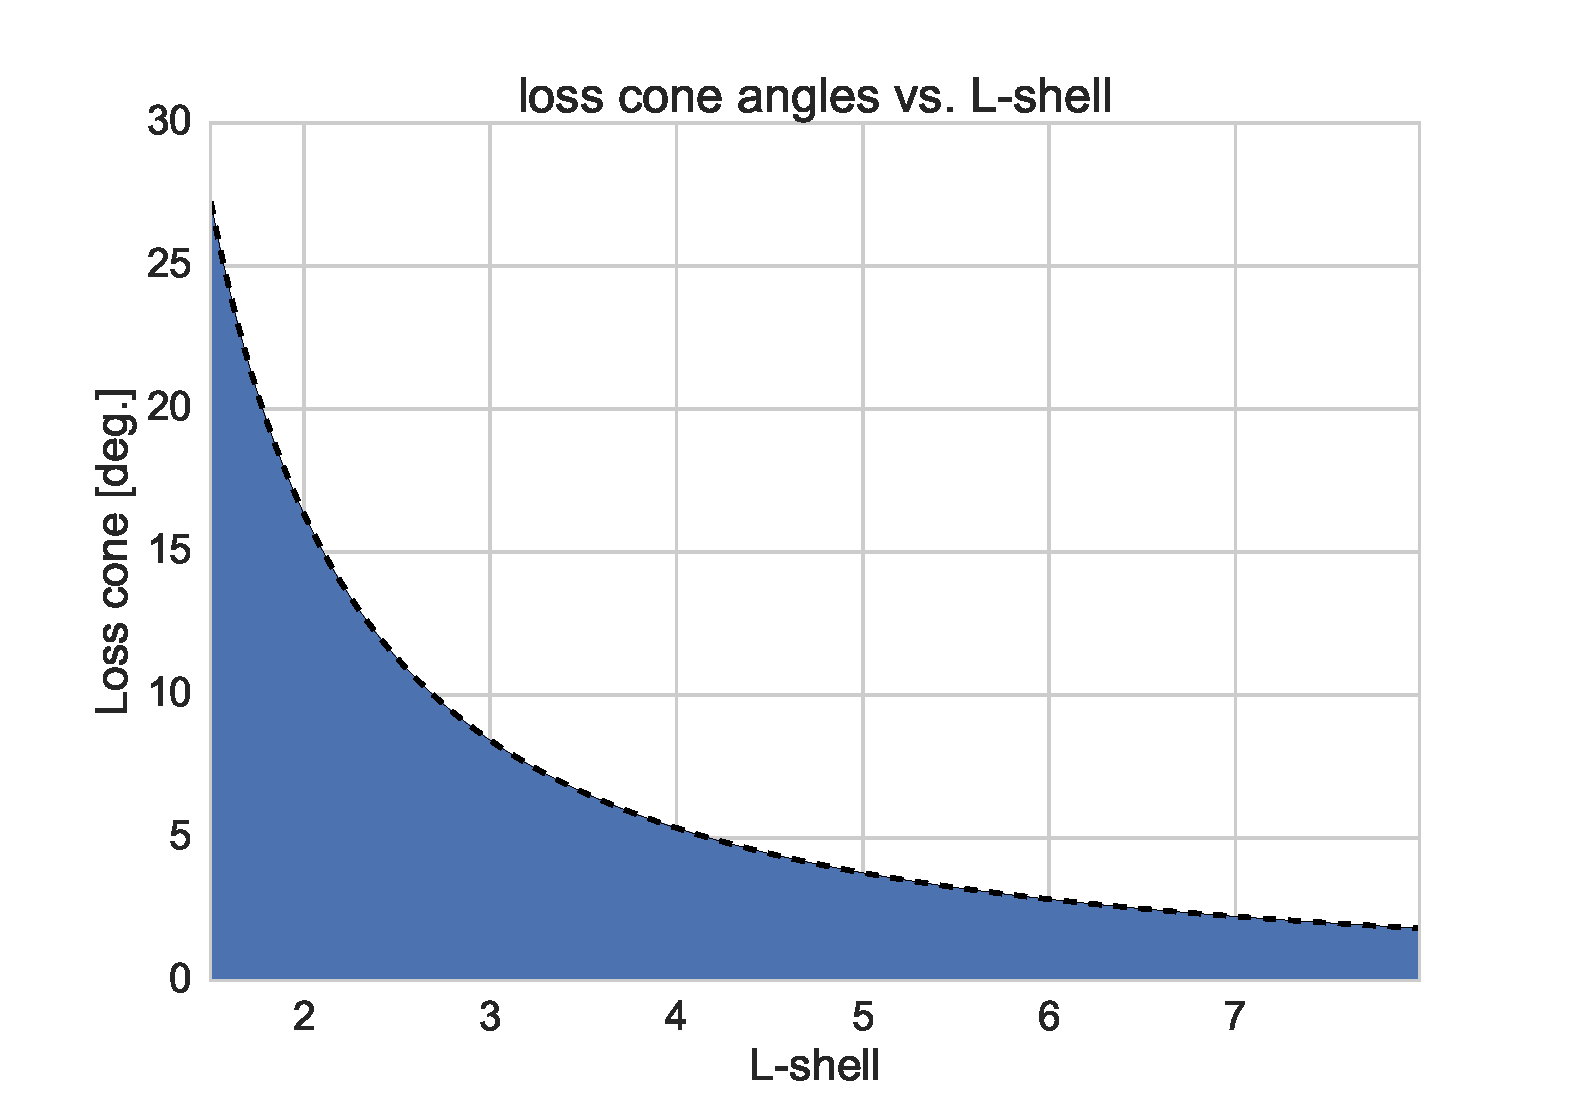
\includegraphics[width=0.8\linewidth]{gfx/lossconeangle}
	\caption{Shaded area indicates loss cone width vs. L-shell}\label{fig:losscone}
\end{figure}
Mirroring particles that are accelerated along $B$ experience an increase in $v_\parallel$ and a decrease in $\alpha_p$, increasing the likelihood the accelerated population will precipitate into the ionosphere and create aurora.
Some important L-shells for Earth are:
\begin{itemize}
	\item nightside plasmapause: 3.5 (active) to 5 (quiet)
	\item inner Van Allen Belt: 1.03 (SAA) to 3
	\item auroral oval: 4..6
\end{itemize}

\section{Auroral Energy Deposition}
The dynamic solar wind drives variability in planetary aurora at Venus \citep{phillips1986,gerard2008}, Earth, Mars \citep{bisikalo2017}, Jupiter, Saturn \citep{kivelson2005}, Uranus and Neptune \citep{arridge2015}.
Aurora at the Galilean moons are primarily driven by the Jovian magnetosphere \citep{lavrukhin2015,roth2016}.
Given the vast differences in scale, distance from the sun and plasma densities and composition, the processes in the auroral lifecycle are distinct for each planetary body.
At Earth, although some particles from the solar wind stream into the dayside geomagnetic cusp, this dissertation focuses on structured nightside aurora that is indirectly related to the solar wind loading of the magnetosphere.

The largest source of energy driving ionospheric variability at Earth is the solar wind.
The solar wind flux is filtered and stored in the magnetotail through heterogeneous and highly time-varying magnetospheric interfaces and regions.
Studies of finely structured aurora begin with data inversion from radar and optical sensors to build understanding of the auroral acceleration region dynamics. 
\textit{In situ} measurements from dense networks of on-orbit magnetometers such as ANDESITE \citep{parham2016} reveal fine current structure in the upper ionosphere.
On-orbit particle detectors such as FAST and DMSP as well as rocket borne particle detectors have been fundamental to confirming and updating theory for over 50 years.
An ultimate goal of geospace studies is to understand Earth's interaction with the solar wind as an entire system with an energy budget across scales and regions.
An ensemble of instruments study the geospace system regions at various scales. 
This dissertation examines auroral microstructure to reveal the acceleration mechanism driving the aurora.
The results may be used in the future to understand fine current structures at other planetary bodies via theory enhancement and may guide development of future instruments for use on Earth and beyond.

The solar wind peak input flux to the Earth's magnetosphere can exceed $\unit[10^{12}]{W}$ \citep{akasofu1980}.
Intense auroral precipitation of over $\nicefrac{1}{4}$ terawatt and Joule heating of several terawatts result in a diverse set of ionospheric responses \citep{lu2016}.
Given the complicated nature of energy coupling from the heliosphere through the interfaces and regions leading to dissipation in the ionosphere, a plurality of models have evolved over the past century.
A basic model for substorm auroral energy flow is depicted in Figure~\ref{fig:auroralenergy}, with a contemporary substorm model diagram in Figure~\ref{fig:collapse}.
\begin{figure}\centering 
    %the \par is necessary after each text to make the \baselineskip take effect
    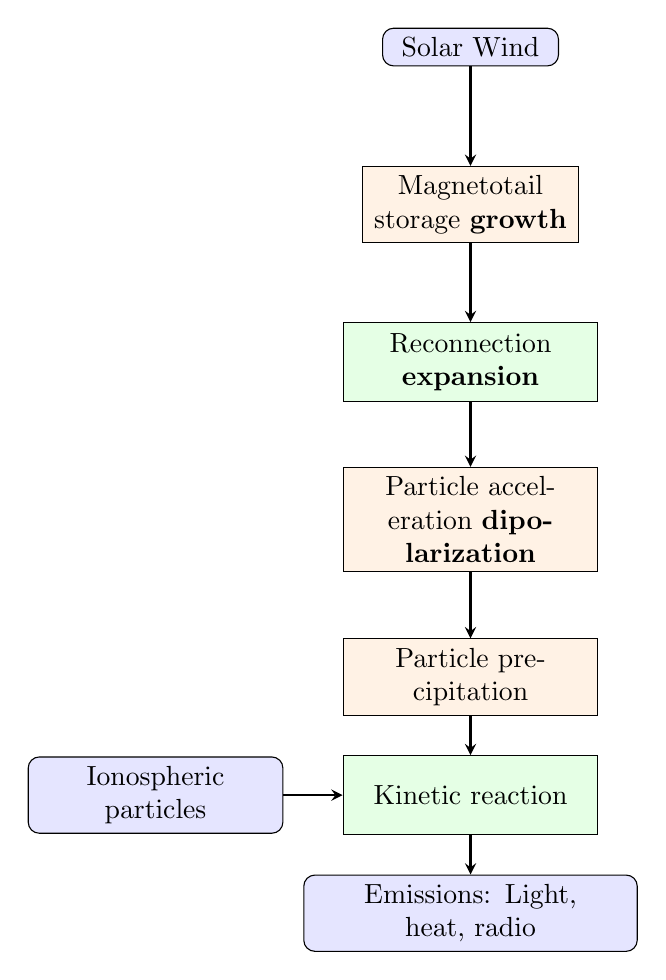
\begin{tikzpicture}[node distance=1.5cm, auto]
    
    \node (in) [startstop,text width=2cm] {Solar Wind \par};
    
    \node (tail) [process, below of=in,text width=2.5cm,yshift=-0.5cm] { Magnetotail storage \textbf{growth}\par };
    
    \node (recon) [compute,below of=tail,text width=3cm,yshift=-0.5cm] { Reconnection \textbf{expansion} \par };
    
    \node (accel) [process, below of=recon, text width=3cm,yshift=-0.5cm] {Particle acceleration \textbf{dipolarization}\par };

	\node (precip) [process, below of=accel,text width=3cm,yshift=-0.5cm] { Particle precipitation \par};
	
	\node (kinetic) [compute, below of=precip,text width=3cm] { Kinetic reaction \par};
	\node (neutral) [startstop, left of=kinetic,text width=3cm,xshift=-2.5cm] {Ionospheric particles \par};
	
	\node (end) [startstop, below of=kinetic,text width=4cm] { Emissions: Light, heat, radio  \par};
    
    \draw[arrow] (in) -- (tail);
    \draw[arrow] (tail) -- (recon);
    \draw[arrow] (recon) -- (accel);
    \draw[arrow] (accel) -- (precip);
    
    \draw[arrow] (neutral) -- (kinetic);
    \draw[arrow] (precip) -- (kinetic);
    
    \draw[arrow] (kinetic) -- (end);

    
    \end{tikzpicture}
    
    \caption{Simplified model for substorm auroral energy dissipation during southward IMF, adapted from \citet{baker1996}.}
    \label{fig:auroralenergy}
\end{figure}
\begin{figure}
	\includegraphics[width=\linewidth]{gfx/substorm-catapult}
	\caption{A substorm model based on \textit{in situ} \citep{machida2009} and optical data \citep{machida2014}.}
	\label{fig:collapse}
\end{figure}
Other important processes involved in long-term evolution of aurora due to ionospheric reconfiguration include Joule heating.
Advances in observational techniques, comparative studies and increased computational power have led to refinements in these models, and this dissertation is another contribution in the observational stack.

\FloatBarrier
\subsection{Particle Loss Mechanisms}
One outcome of the loss of charged particles from the magnetosphere is the production of aurora. 
A primary driver of the finely structured aurora is substorms \citep{fukushima1962,akasofu1964,elphin1996}.
The substorm expansion phase is thought to be driven by reconnection, which is a rapid reconfiguration of open and closed field lines due to their close encounter.
During the expansion phase, a large amount of charged particles and waves are launched toward Earth.
The magnetotail plasma on the far side of the reconnection site known as a plasmoid permanently disconnects from the magnetosphere and drifts anti-sunward from Earth into the solar system. 

Substorms create an impulsive earthward restoration of the magnetotail with some of the energy carried by the Alfvén waves discussed in section \ref{sec:alfven}. 
Quantifying the energy deposition versus ionospheric altitude of precipitating electrons is central to the data inversion of this dissertation in chapters \ref{chapter:sim} and \ref{chapter:fusion}. 
Following \citet{rees1989}, we use the laboratory results of \citet{barrett1976} valid for 300..\unit[5000]{eV} that used the apparatus in Figure~\ref{fig:BellJar} to obtain
\begin{equation}\label{eq:empiricalRange}
R_{\textrm{e}^-} = 4.30 + 53.6\phi^{1.67}_{E_i}  \quad \textrm{ kg-m$^{-2}$} 
%\marginnote{e\textsuperscript- mass distance in N$_2$}
\end{equation} %Barrett & Hays p. 748
%\fxnote{Dropping the last term brings error to $10^{-8}$ from $10^{-3}$}
%\citep{JLSrs2005}  $R_{e^-} = 4.3 + 53.6K_i^{1.67} - -0.038K_i^{-0.7} \textrm{ kg-m$^2$}$} matches within 1-e3
the electron mass distance in N$_2$. 
Figure~\ref{fig:empR} shows \eqref{eq:empiricalRange}  extrapolated to energies observed at ionospheric altitudes instead of using the more complicated first principles transport equations. %paragraph 9
\begin{figure}\centering
    \includegraphics[width=0.8\textwidth,trim=30 10 30 20,clip]{gfx/JLSkamalabadiEqn2.eps}
    \caption{Mass-range according to \citet{semeter2005}}\label{fig:empR}
\end{figure}
The electron scattering depth for altitude $z$ is
\begin{equation}\label{eq:satm}
s_{\textrm{atm}} = \sec{\left( \theta_B \right)}\int_z^\infty \rho(z)\textrm{d}z \quad \textrm{ kg-m$^{-2}$} 
%\marginnote{e\textsuperscript- scattering depth}
\end{equation}
\citep{semeter2005}, where $\rho(z)$ is the mass density as obtained from the MSIS model. 

The maximum mass distance of the electron is $R_{\textrm{e}^-} = \pm 1$. The range $1 \leq R_{\textrm{e}^-} < 0$ accounts for backscattered electrons reflected back up toward the magnetosphere. 
An electron that travels mass distance $\Delta(s/R)$ loses $\Delta(E/\phi_{E_i})$ fraction of the initial energy. 
In the limit as $\Delta(s/R) \rightarrow 0$, the energy dissipation function
\begin{equation}\label{eq:energyDissFunc}
\Lambda = \frac{\mathrm{d}E/\phi_{E_i} }{ \mathrm{d}s/R }
\end{equation}
is defined \citep{semeter2005}. 
The energy dissipation function 
\begin{equation}\label{eq:qioniz}
q\left( z,\phi_{E_i} \right) = F \phi_{E_i} \Lambda \frac{\rho(z)}{R_{\textrm{e}^-}} \frac{1}{\Delta\varepsilon_{\textrm{ion}}}
\end{equation}
forms the core of the total ionization rate due to a precipitating electron beam \citep{rees1989}.
The average $\Delta\varepsilon_{\textrm{ion}}$ is typically taken \citep{semeter2005} to be \unit[35.5]{eV}.

We are interested in the contribution to $q$ of the differential flux $\Delta F$ impinging on the ionosphere with uniformly distributed energy range $\phi_{E_i} + \Delta\phi_{E_i}$. 
This is expressed in differential form \citep{semeter2005} 
\begin{equation}\label{eq:FredKernEner}
q\left( z,\phi_{E_i} \right) = \int_{\phi_{E_i}}^{\phi_{E_i}+\Delta\phi_{E_i}} \left[ \frac{\Lambda\rho\phi_{E_i} }{ \Delta\varepsilon_{\textrm{ion}} R } \right] \mathrm{d}\phi(E_i)d\phi
\end{equation}
where $\Delta F$ is represented by $\phi(E_i)\mathrm{d}E_i$. 
The differential system solution is aided by representing~\eqref{eq:FredKernEner} using the FIEFK
\begin{equation}\label{eq:JLSfiefk}
q(z) = \int_{E_{i,\textrm{min}}}^{E_{i,\textrm{max}}} A(z,E_i)\phi(E_i)\textrm{d}E_i
\end{equation}
where $A$ encompasses the energy deposition terms. 
The input differential number flux over all pitch angles $\phi(E_i)$ is the quantity estimated by the HiST system as described in chapter~\ref{chapter:sim}. 

%TODO $\phi$ is flux, not energy. Be sure it's consistent here.

\FloatBarrier
\subsection{Kinetic Reaction Outcomes}
A substantial fraction of the electrons precipitating from the magnetosphere into the ionosphere react kinetically with ionospheric particles in the \unit[90]{km} to \unit[500]{km} altitude range.
The electron precipitation flux incident on the top of the ionosphere as a function of energy $E$ is denoted as $\phi_{\mathrm{top}}(E)$ \citep{rees1989}.
A substantial fraction of the incident energy is reflected back to the magnetosphere according to the ionospheric albedo.
Albedo is equivalent to the reflection coefficient of a mismatched transmission line between the magnetosphere and ionosphere.
Secondary electrons produced by impact ionization in the ionosphere can reflect back into the magnetosphere.
This secondary electron population mirrors into the outer plasma with flux sufficient to heat the outer plasmasphere and hence significantly influence the conjugate ionospheric state \citep{khazanov2014}.
The kinetic reaction outcomes most relevant to ionospheric microscale features include unstable wave growth, ionospheric turbulence and the associated auroral microstructure.
An overview of the outcomes of ionospheric kinetic reactions are represented in Figure~\ref{fig:auroragen}, with a more detailed look at conditions favorable for auroral microstructure in Figure~\ref{fig:alfvenblock}.
\begin{figure}\centering
	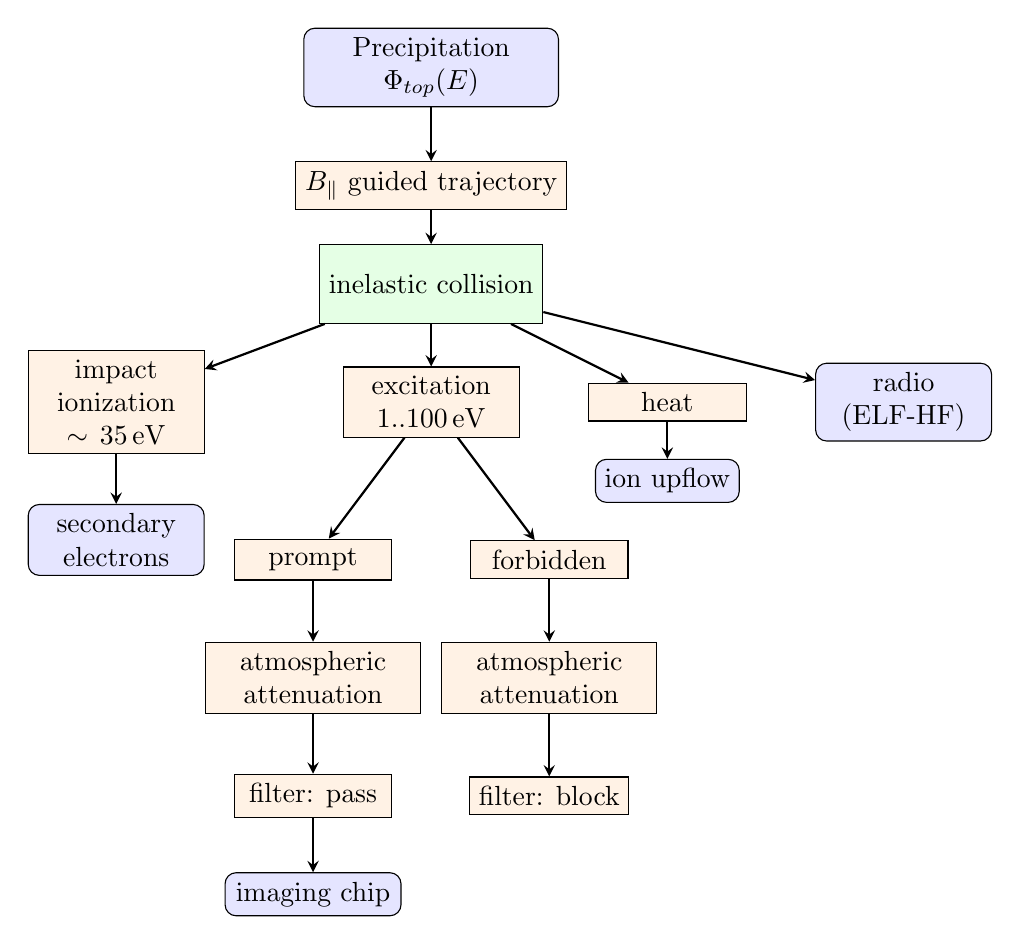
\begin{tikzpicture}
	\node (precip) [startstop,text width=3cm] {Precipitation $\Phi_{top}(E)$ \par };
	
	\node (B) [process,below of=precip,yshift=-0.5cm] {$B_\parallel$ guided trajectory \par};
	
	\node (bang) [compute,below of=B,yshift=-0.25cm] {inelastic collision \par};
	
	\node (exc) [process,below of=bang,yshift=-0.5cm,text width=2cm] {excitation \unit[1..100]{eV} \par};
	\node (prompt)[process,below of=exc,xshift=-1.5cm,yshift=-1cm]{prompt \par};
	\node (forb)[process,right of=prompt,xshift=2cm]{forbidden \par};
	
	%\node (diss)[process,left of=exc,xshift=-2cm]{ dissociation \par};
	\node (ioni)[process,left of=exc,xshift=-3cm,text width=2cm] { impact ionization $\sim \unit[35]{eV}$ \par};
	\node (heat)[process,right of=exc,xshift=2cm] { heat \par};
	\node (radio)[startstop,right of=heat,xshift=2cm,text width=2cm]{ radio (ELF-HF) \par};
	
	\node (upflow)[startstop,below of=heat]{ion upflow \par};
	
	\node(secondary) [startstop,below of=ioni,yshift=-0.75cm,text width=2cm] {secondary electrons \par};
	
	\node (patt)[process,below of=prompt,text width=2.5cm,yshift=-0.5cm]{ atmospheric attenuation \par};
	\node (pass)[process,below of=patt,yshift=-0.5cm]{ filter: pass \par};
	
	\node (fatt)[process,below of=forb,text width=2.5cm,yshift=-0.5cm]{ atmospheric attenuation \par};
	\node (block)[process,below of=fatt,yshift=-0.5cm]{ filter: block \par};
	
	\node (chip)[startstop,below of=pass,text width=2cm,yshift=-0.25cm] {imaging chip \par};
	
	
	\draw[arrow] (precip) -- (B);
	\draw[arrow] (B) -- (bang);
	
	\draw[arrow] (bang) -- (exc);
	\draw[arrow] (bang) -- (ioni);
	%\draw[arrow] (bang) -- (diss);
	\draw[arrow] (bang) -- (heat);
	\draw[arrow] (bang) -- (radio);
	
	\draw[arrow] (ioni) --(secondary);
	
	\draw[arrow] (heat) -- (upflow);
	
	\draw[arrow] (exc) -- (prompt);
	\draw[arrow] (prompt) -- (patt);
	\draw[arrow] (patt) -- (pass);
	\draw[arrow] (pass) -- (chip);
	
	\draw[arrow] (exc) -- (forb);
	\draw[arrow] (forb) -- (fatt);
	\draw[arrow] (fatt) -- (block);
	
	\end{tikzpicture}
	\caption{Block diagram of auroral optical emissions generation and observation.
	The \texttt{filter} blocks represent emissions that are passed or blocked by HiST bandstop filtering.}
	\label{fig:auroragen}
\end{figure}


\FloatBarrier
\subsection{Radar Probing of Ionospheric Turbulence}
Two of the elementary electrostatic plasma wave modes discovered and characterized by \citet{tonks1929} \citep{hershkowitz2009} with the apparatus of Figure~\ref{fig:langmuirtube}  are the ion-acoustic wave and Langmuir (electron-acoustic) wave, with $\vect{k} \parallel \vect{B}$.
\begin{figure}
	\includegraphics[width=\linewidth]{gfx/langmuir-tube}
	\caption{Apparatus used by Langmuir in \citet{tonks1929} to characterize several ion and electron plasma waves.}
	\label{fig:langmuirtube}
\end{figure}
The dispersion relation for Langmuir waves is
\begin{equation}
\omega ^{2} = \omega _{pe}^{2}+3/2 k^{2}v_{e}^{2}
\end{equation}
where electron thermal velocity 
\begin{equation}
v_e = \sqrt{2 \frac{T_0}{m_e}}
\end{equation}
and $T_0$ is the temperature of the unperturbed cold plasma background.
If we suppose that background cold plasma density $n_0$ is small or that $k_\parallel$ is small, the typical observation of ISR plasma line frequency $\omega \sim \omega_{pe}$ is realized \citep{akbaridis}.
The dispersion relation for ion-acoustic waves is
\begin{equation}
\omega ^{2} = k^{2}{\frac{k_B(T_{e} + 3 T_{i})}{m_i}}
\end{equation}
and this gives rise to the ``ion line'' as depicted in Figure~\ref{fig:isrmorph}, from which the plasma parameters $n_e, T_e, T_i, v_i$ can be estimated by ISR \citep{swobodathesis}.

Very strong radar scattering can occur at radar frequency $\omega_0 \gg \omega_{pe}$, where plasma frequency is \citep{langmuir1928,chenbook}
\begin{equation}\label{eq:wpe}
\omega_{pe} = \sqrt{\frac{n_e e^2}{\epsilon_0 m_e}}.
\end{equation}
Although phase shift is expected for $\omega > \omega_{pe}$, a fact exploited in the use of GNSS TEC measurements \citep{coster1992}, constructive reflections from a sufficiently large power aperture radar yield a detectable signal.
Other minuscule signals detectable with ISR include meteoric smoke particles \citep{mahmoudian2017,baumann2016,hsu2011} and space debris down to \unit[3]{cm} at \unit[1000]{km} range with \unit[100]{ms} integration time \citep{nicolls2015}.
Almost as soon as PFISR was turned on, naturally enhanced ion acoustic lines (NEIALs) were observed, which \citet{michell2008} in Figure~\ref{fig:firstpfisrneials} associated with bright auroral forms.
\begin{figure}
	\includegraphics[width=\linewidth]{gfx/pfisrfirstneials}
	\caption{NEIALs and correlated optical intensity rise observed with the PFISR magnetic zenith beam in March 2006 \citep{michell2008}.}
	%Note, wavelength was not given in the paper. I know it's NOT the sum of all lines, but not sure which line. Probably 557.7 is my guess. Could find out from original P-DMSP data.
	\label{fig:firstpfisrneials} 
\end{figure}
NEIALs are the ISR observed results of Bragg scattering from plasma turbulence at 1/2 the radar wavenumber, leading to the ion line spectra of Figure~\ref{fig:isrmorph}(b,c).
NEIALs have been observed to occur over 140..\unit[1900]{km} altitude range \citep{schlatter2013}.





%Langmuir waves are electrostatic plasma waves where $\omega \sim \omega_{pe}$. 

%\citet{newman1994linear} notes that Langmuir bursts occur in ``moderately magnetized'' plasma where $\Omega_e \approx \omega_{pe}$.
%\citet{akbari2013} connected HF emissions in the 0.1..\unit[10]{MHz} range with NEIALS.





\section{Auroral Emissions}\label{sec:physicsemissions}

Given the historical record of deep red aurora observable at latitudes at least as low as $10^\circ$ \citep{silverman2008}, many nations and cultures have experienced aurora at least once a generation.
A rule of thumb for naked-eye visible aurora is the energy flux must be at least $\unit[1]{mW\, m^{-2}}$ or a volume emission rate greater than \unit[1]{kR}.
Modern semiconductor-based photoelectron-multiplying imaging chips give wide dynamic range and industry-leading single-photoelectron sensitivity, revealing detailed auroral features at intensities far below what human eyes and emulsified film can accomplish at high frame rates.
Purple aurora thought to correspond to \unit[427.8]{nm} and \unit[391.4]{nm} emissions is occasionally seen at the lower edge of auroral displays, when the viewing geometry and conditions are such that it is not overwhelmed by the far more intense \unit[557.7]{nm} and \unit[630.0]{nm} emissions.
%TODO This paper has info on cross sections
%\url{https://www.nist.gov/sites/default/files/documents/srd/jpcrd387.pdf}

The notional auroral spectrum in Figure~\ref{fig:VJaurora} shown over the wavelength span of interest is for a bright ICB III aurora.
\begin{figure}
	\includegraphics[width=\textwidth,trim=5 10 5 1,clip]{gfx/AuroralSpectrumLogVJ}
	\caption{Auroral spectrum in wavelength range of interest, from \citet{vallancejones1974}. }\label{fig:VJaurora}
\end{figure}
To reject metastable emissions with lifetime $\tau \gg\unit[1]{ms}$ that would smear out prompt auroral emissions, the DMC and HiST systems observed through Schott BG3 bandstop filters with specified performance in Figure~\ref{fig:BG3trans}. 
\begin{figure}\centering
	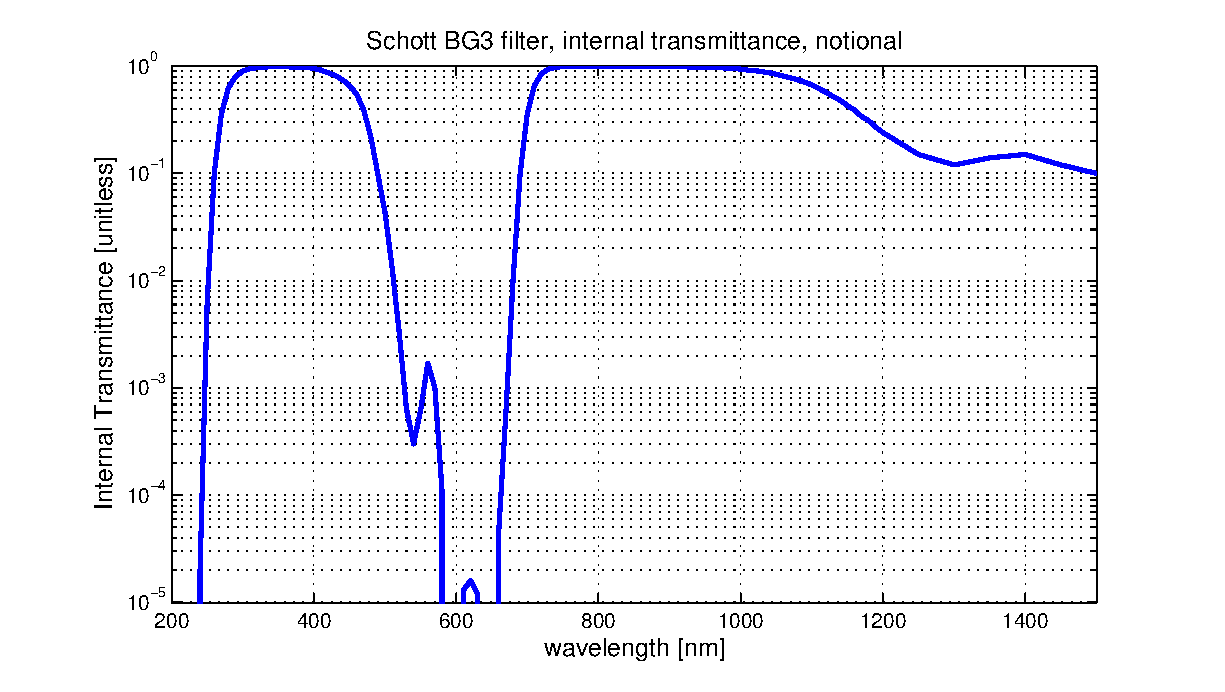
\includegraphics[width=\textwidth]{gfx/BG3transLog}
	\caption{Schott BG3 filter response}\label{fig:BG3trans}
\end{figure}
A comparison of the BG3 filter with historical and contemporary prompt emissions filters is given in Figure~\ref{fig:filters}.
The deep notch in the BG3 spectral response rejects most intense long-lifetime emissions. 
The notional EMCCD window transmission and Quantum Efficiency (QE) are shown in Figure~\ref{fig:EMCCDwindQE}.
\begin{figure}\centering
	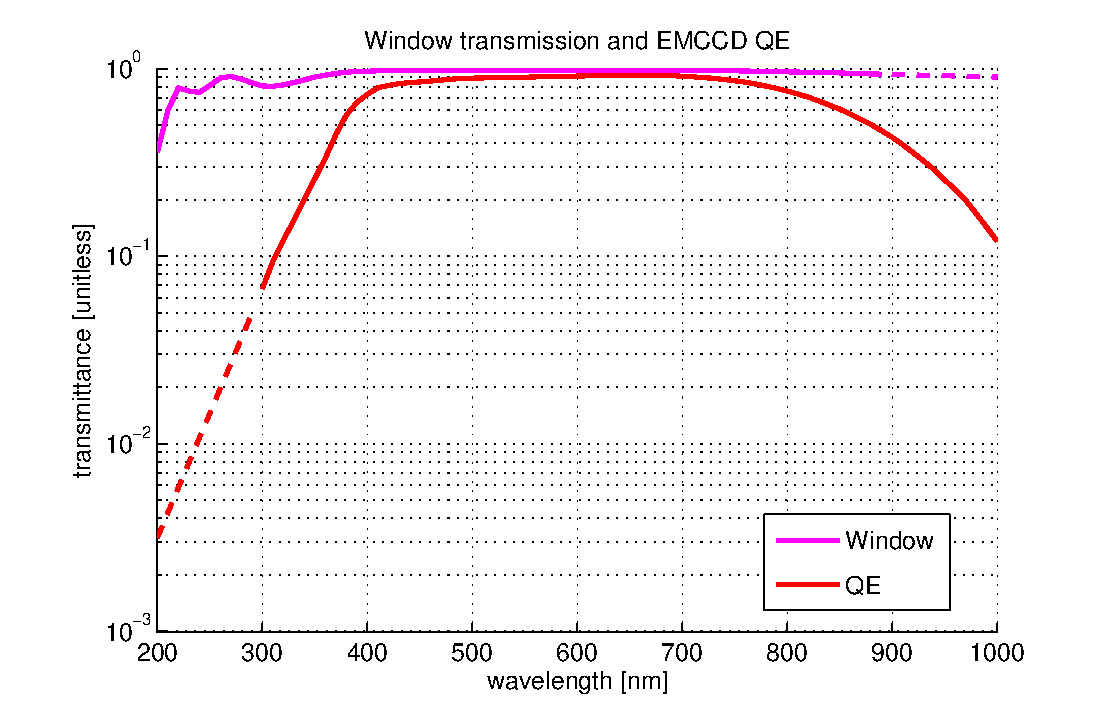
\includegraphics[width=\textwidth]{gfx/EMCCDwindowQELog}
	\caption{EMCCD window transmission and QE (extrapolated values dashed)}\label{fig:EMCCDwindQE}
\end{figure}  
The notional total system response in the wavelength range $\lambda \in [200,1000]$ nm is shown in Figure~\ref{fig:systemSpectralResp}.
\begin{figure}\centering
	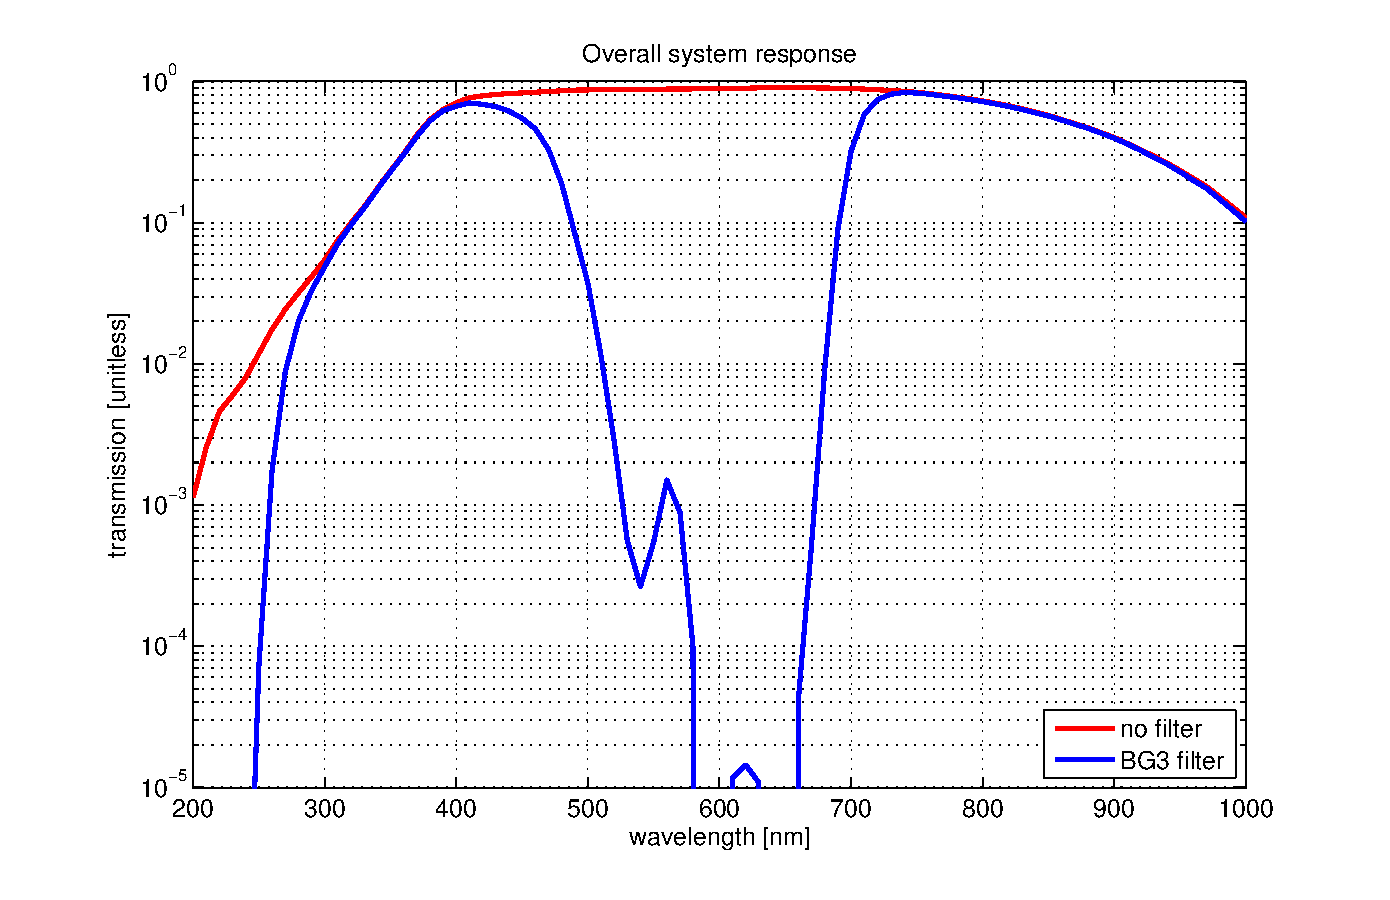
\includegraphics[width=\textwidth]{gfx/EMCCDoverallTlog}
	\caption{Overall optical transmission from lens through EMCCD chip}\label{fig:systemSpectralResp}
\end{figure}
The overall HiST transmission including atmospheric absorption, particularly significant at UV is shown in Figure~\ref{fig:optTrans}.
Several well-known auroral emission lines are given in Table~\ref{tab:spectrum} along with the optical system attenuation noted in Figure~\ref{fig:auroragen}. 

Brightness observed for the \unit[427.8]{nm} line, often taken as a proxy for high-energy precipitation has been given in the \unit[0.1..3]{kR} range \citep{dashkevich2006}.
% below 150km, dissociative recombination becomes important
Typical parameters for auroral flux as given by \citet{sandholtbook} are in Table~\ref{tab:typaurora}.
\begin{table}\centering
	\caption{Notional auroral emissions characteristics~\citep{sandholtbook}.}
    \label{tab:typaurora}
	\begin{tabular}{clll}
        \toprule
		wavelength [nm] & state & excitation energy [eV] & peak alt. [km] \\
		\midrule
		630.0 & [O] ($^1$D) & $\sim5.6$ & 200 \\
		557.7 & [O] ($^1$S) & $\sim10$ & 120 \\
		427.8 & N2$^+$ 1N & $\sim 100$ & 100 \\
        \bottomrule
	\end{tabular}
\end{table}
A starting point for the notional particle flux is typically of order $\unit[10^{13}]{m^{-2}s^{-1}}$ with energy flux of order $\unit[10]{mW \,m^{-2}}$.
A classic technique for estimating characteristic intensity $E_0$ looking up the magnetic zenith flux tube is based on the intensity ratio of line spectra.
From \citet{rees1974}, the typical ratio of $I_{6300}/I_{4278}$ is about 0.05..15, for $I_{6300}/I_{5577}$ the typical ratio is about 0.03..2.
However, for structured aurora these ratioing techniques fall apart (become highly inaccurate) since they completely lose validity away from magnetic zenith. 
%TODO justify this assertion!
An auroral observation system capable of observing within several degrees of magnetic zenith is necessary to quantify the differential number flux $\Phi_{top}$ driving structured aurora.
HiST is the first such system capable of estimating auroral precipitation characteristics with \unit[20]{ms} cadence, a rate compatible with the fastest ISR measurements as described in chapter~\ref{chapter:fusion}.

	

\section{Small scale auroral features and Alfvén waves}
Starting in the 1950s and 1960s, auroral morphology from the polar regions and auroral oval down to the mid latitudes \citep{akasofu1963} was rigorously studied.
The discovery of the magnetosphere and early understanding of its processes and regions by the mid-1960s hastened the instrument development cycle, both space- and ground-based.
Descriptions of auroral morphology depend strongly on the viewing perspective due to~\eqref{eq:bint}.
The viewer directly beneath the aurora of Figure~\ref{fig:chernouss6}(a) sees ribbons of aurora while the viewer roughly \unit[100]{km} away sees auroral curtains in Figure~\ref{fig:chernouss6}(b)--despite looking at the same section of aurora.
To motivate the disentangling of this difficult observational problem in chapter~\ref{chapter:sim}, a discussion of the processes driving microscale aurora is in order.

Despite the highly complex and time-varying linkages and paucity of coördinated \textit{in situ} measurements, a first step in understanding a ``black box'' system is quantifying the energy flux for the system and its components.
Cold ionospheric plasma, mirroring particles, the plasma sheet and direct injection from the solar wind are among  ultimate sources of precipitating particles driving the aurora.
Particle momentum carries particles across the solar system, with shocks and pickup ions redirecting the guiding center trajectory.
The structure of structured aurora is oriented along the $B_\perp$ dimension due to the frozen-in condition of plasma causing the guiding center of particles to follow geomagnetic field lines.
Structured aurora is a projection of acceleration structures in the 3000..\unit[10000]{km} altitude range.
When discussing the atmosphere, ionosphere and magnetosphere, altitude is given above mean sea level.
The finest ground-observable structures are of order \unit[10..100]{m} from even filamental electron beams due to diffusion in the ionospheric column traversed \citep{borovsky1993}.

Throughout this dissertation, ``ion'' is synonymous with a particle of positive charge. Some of the important species in the ionosphere include N$_2$, O, and N$_2^+$. 
While solar radiation throughout the ultraviolet (UV) range is responsible \citep{rees1989} for creating much of the plasma in the ionosphere, accelerated electrons are the primary driver of the aurora. 
Assumptions used in the analysis include:
\begin{enumerate}
    \item Precipitating electron energies $E > \unit[100]{eV}$
    \item Average energy loss per ionization is \unit[35.5]{eV}
    \item Excitation requires energy \unit[1..100]{eV}
%    \item \citep{semeter2005} %paragraph 17
\end{enumerate}
``Cold'' ionospheric plasma has energies of a few eV, much less than the 35~eV needed to emit a photon.
Solar wind particles have energies of order \unit[100]{eV} \citep{mottez2015}.
Only about 1\% of the $1.3 \times 10^{13}$~W flux intercepting Earth's magnetosphere is captured into the magnetosphere system \citep{mottez2015}.
Most of the intercepted flux is stored in the magnetotail, which explosively discharges every several hours in substorms, taking a few hours to restore the magnetosphere to a relaxed state, which is already recharging with solar wind flux for the next cycle.
The shear forces and turbulence in general associated with reconfiguration in any magnetic system must be communicated to other portions of the magnetoplasma.
Alfvén waves are a key mechanism for releasing stress in dynamic magnetoplasma systems.

\FloatBarrier
\subsection{Alfvén Waves}\label{sec:alfven}
Plasmas infused with magnetic field $B$ are subject to perturbations that send energy across vast distances.
On intergalactic scales, Alfvén waves have been thought to have a possible role in the evolution of cosmic rays \citep{matsukiyo2009}.
In the solar wind, theory and modeling have shown a possible role in instabilities leading to filamentation of Alfvén waves and corresponding perturbations in plasma density and $B$ \citep{kuo1988}.
In the geomagnetic system, stresses and reconfigurations from geomagnetic storms and substorms are communicated with speeds reaching to order $0.1c$. 
Alfvén waves communicate information about the constantly reconfiguring geomagnetic system across scales and great distances.

In general Alfvén waves may propagate obliquely to $B$, but for observable outcomes of electron acceleration by Alfvén waves, we assume that the Alfvén wave electric field is oriented approximately parallel to $B$.
The fingerprints of Alfvénic aurora due to Alfvén wave electron acceleration may be seen in measurements back at least to the 1970s.
The theory and modeling were solidified in the 2000s by works such as \citet{stasiewicz2000,chaston2003,chaston2007how}.
Although large fluxes of Alfvén wave-accelerated electrons in the \unit[1..10000]{eV} range are responsible for many dramatic structured auroral displays \citep{chaston2003}, numerous other methods of auroral acceleration exist \citep{borovsky1993}.

Waves in media may have fields oriented longitudinally, transverse, or oblique to the direction of propagation $\hat{k}$. 
Longitudinal waves are also known as \textit{compression} waves and transverse waves are also known as \textit{shear} waves.
Alfvén waves can reflect off the ionosphere and plasma sheet in the magnetotail repeatedly. 
Instabilities generated in ionospheric plasma by Alfvén waves have been shown by observation and modeling to be a plausible candidate for ion upflow \citep{chaston2004}, without directly involving heating \citep{zett2007,zett2008}.
Subsets of IAW such as solitary IAW and dissipative nonlinear IAW have been proposed as consistent with narrow auroral features \citep{wu2004}.
Alfvén waves have been shown to be a primary driver of dynamic aurora via \textit{in situ} observations including DMSP and FAST measurements compiled over several years.
As recounted in \citet{stasiewicz2000}, Hannes Alfvén's development and the observational confirmation of Alfvén wave theory parallels that of J. C. Maxwell's elucidation of electromagnetism.
Distinguishing between intra-Alfvénic and non-Alfvénic wave electron acceleration, essential to the $B_\perp$ structure of kinetic plasma behavior, is enhanced by the equipment described in chapter~\ref{chapter:inst} and analysis in chapters~\ref{chapter:sim} and~\ref{chapter:fusion}.

The electron thermal velocity is
\begin{equation}
v_{te} = \sqrt{2\frac{T_e}{m_e}}
\end{equation}
while Alfvén waves propagate with Alfvén velocity
\begin{equation}
v_A = \frac{B_0}{\sqrt{\mu_0\rho}}
\end{equation}
and Alfvén wave frequency
\begin{equation}
\omega = k_\parallel v_A
\end{equation}
where $v_A \ll c$ in many geomagnetic plasmas, $T_e$ is electron temperature, $m_e$ is the electron mass, $\rho=n_im_i$ is the mass density, $B_0$ is the local geomagnetic field strength and $\mu_0$ is the vacuum permeability \citep{stasiewicz2000}.
As $v_A \Rightarrow c$, the Alfvén wave behaves increasingly as if in a non-magnetized medium.
The rules of phase reversal upon reflection are the same for Alfvén waves as for general TEM waves.
Two Alfvén wave regimes referred to collectively as dispersive Alfvén waves (DAW) are described in Table~\ref{tab:alfven} and section~\ref{sec:alfvenaccel}.
\begin{table}\centering
	\caption{Dispersive Alfvén wave types relevant to auroral acceleration \citep{stasiewicz2000}.}
    \label{tab:alfven}
	\begin{tabular}{ccccc}
        \toprule
		Alfvén wave type & frequency & speed & pressure & altitude [km] \\
		\midrule
		inertial & $\omega < \omega_{ci}$  & $v_A > v_{te} $  & $ \beta < \frac{m_e}{m_i} $ & 3,000..20,000 \\ % Staciewicz 2001 pg. 429
		kinetic & & $v_A < v_{te}$ & $\frac{m_e}{m_i} < \beta < 1$ & $\gtrsim 20,000$ \\
        \bottomrule
	\end{tabular}
\end{table}


\FloatBarrier
\subsection{Alfvénic Auroral Acceleration}\label{sec:alfvenaccel}
Electron-driven aurora can most broadly be categorized as diffuse or discrete \citep{newell2009}.
Diffuse and structured auroral arcs driven by inverted-V potential structures may be time-modulated in flux by ion-acoustic resonances.
Regions with sharp potential gradients are included in the category of inverted-V precipitation driven aurora, along with the smoothly varying potential structure the name implies \citep{newell2009}.
Inverted-V arcs may translate, but they do not experience splitting or flaming behavior, and NEIALs are not associated with them.
The diffuse aurora life cycle is dominated by resonant wave-particle interactions scattering plasma sheet electrons in the loss cone \citep{Ni2016}.
Time-modulated diffuse aurora is driven by mechanisms with little dispersion relative to discrete auroral drivers.
\begin{figure}\centering
	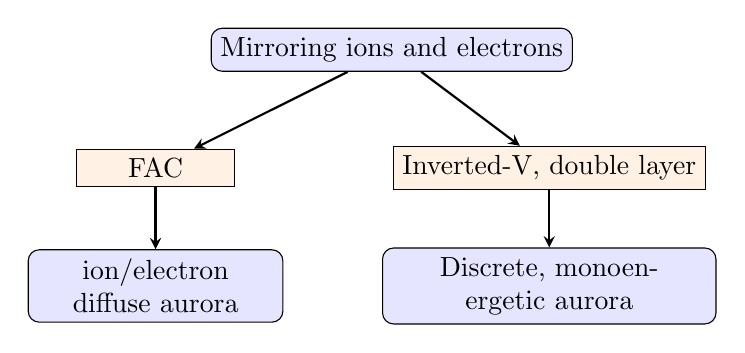
\begin{tikzpicture}
	\node (mirror) [startstop] {Mirroring ions and electrons \par };
	
	\node (fac) [process,below of=mirror,xshift=-3cm,yshift=-0.5cm] {FAC \par};
	
	\node (ion) [startstop,below of = fac,text width=3cm,yshift=-0.5cm] {ion/electron diffuse aurora \par};
	
	\node (inv) [process,right of = fac,xshift=4cm] { Inverted-V, double layer \par};
	
	\node (mono) [startstop,below of = inv,text width=4cm,yshift=-0.5cm] { Discrete, monoenergetic aurora \par };
	
	
	\draw[arrow] (mirror) -- (fac);
	\draw[arrow] (fac) -- (ion);
	
	\draw[arrow] (mirror) -- (inv);
	\draw[arrow] (inv) -- (mono);
	
	\end{tikzpicture}
	\caption{Block diagram of non-Alfvénic aurora acceleration mechanism.}
	\label{fig:nonalfvenblock}
\end{figure}

\citet{chaston2007how,mcfadden1999} note that particle acceleration relevant to ground-observable aurora occurs along $B_\parallel$ and occurs in altitude ranges from about 3000..\unit[20000]{km}.
\citet{stasiewicz2000} cited Freja measurements showing that while cold plasma $\sim \unit[5]{eV}$ heavily dominates from 1000..8000~km in the auroral zone and polar cap, in Alfvénic turbulence regions almost no cold electrons exist.
The source of sudden large flux of low energy electrons is thought to come from Alfvén wave acceleration of mirroring electrons into the loss cone.
Alfvén waves operate across a wide range of regimes from accelerating relativistic particles in galaxy clusters \citep{brunetti2004} to the Earth's lower magnetosphere.

%To describe the nature of Alfvén waves responsible for auroral acceleration, we begin with Ohm's Law
%\begin{equation}
%\vect{j} = \sigma \vect{E}
%\end{equation}
%that becomes modified in the plasma surrounding Earth due to the collisionless nature of plasma above the lower ionosphere.
%The magnetohydrodynamic momentum balance equation
%\begin{equation}\label{eq:mhdmomentum}
%\rho \frac{\textrm{d}\vect{v}}{\textrm{d}t} = \rho \left(\frac{\partial\vect{v}}{\partial t} + \vect{v} \cdot \nabla \vect{v}\right) = \vect{j} \times \vect{B} - \nabla p
%\end{equation}
%for ions and electrons are subtracted to obtains the Generalized Ohm's Law \citep{paschmann2003}
%\begin{equation}
%\vect{E}+\vect{v}\times\vect{B} = \eta \vect{j} + \frac{1}{ne}\left(\vect{j} \times \vect{B} - \nabla \cdot p_e\right) + \frac{m_e}{ne^2}\left(\frac{\partial \vect{j}}{\partial t} + \nabla \cdot \left(\vect{j}\vect{v} + \vect{v}\vect{j}\right)\right)
%\end{equation}

An important scale concerning Alfvén waves is the electron inertial length or skin depth \citep{paschmann2003}
\begin{equation}\label{eq:einert}
\lambda_e = c/\omega_{pe}
\end{equation}
which relates to ion inertial length
\begin{equation}
\lambda_i = \lambda_e \left(\frac{m_e}{m_i}\right)^{-1/2}.
\end{equation}
In a notional topside ionosphere using~\eqref{eq:wpe} and~\eqref{eq:einert} and assuming $n_e = \unit[10^{10}]{m^{-3}}$
\begin{equation}
\lambda_e = c \left( \frac{n_e e^2}{\epsilon_0 m_e} \right)^{-1/2} = \unit[53]{m}
\end{equation}
which is consistent with sub-\unit[100]{m} width auroral arc features associated with Alfvénic accelerated electrons.
Another relevant scale (assuming as is usual quasistatic ions) is the Debye length \citep{langmuir1928}
\begin{equation}
\lambda _{D}={\sqrt {\frac {\varepsilon_0 k_B T_e}{n_e e^{2}}}}
\end{equation}
that in the magnetosphere is of order \unit[100]{m}.
Inertial waves are backward waves, where the direction of phase velocity is opposite the wave vector $\overrightharp{k}$.
The $\vect{E} \parallel \vect{B}$ field is supported by the electron inertia \citep{stasiewicz2000}.
The dispersion relation for inertial Alfvén waves (IAW) is \citep{stasiewicz2000}
\begin{equation}\label{eq:dispiaw}
\omega^2 = \frac{k^2_\parallel v^2_A}{1+k^2_\perp \lambda^2_e}.
\end{equation}
Using the definition of group velocity we obtain \citep{stasiewicz2000}
\begin{equation}
\frac{\partial \omega}{\partial \vect{k}} = \widehat{z} \frac{v_A}{\sqrt{1+k^2_\perp \lambda_e^2}} - \widehat{x} \omega \lambda_e \frac{k_\perp \lambda_e}{1+k^2_\perp \lambda_e^2}
\end{equation}
which essentially says that the Alfvén wavelength increases with time along $B_\perp$ while accelerating electrons along $B_\parallel$.
The DAW propagates in a conical region with apex angle \citep{semeter2008}
\begin{equation}
\tan \theta_a = \frac{\omega}{\omega_{ci}} \sqrt{\frac{m_e}{m_i}},
\end{equation}
%In left-handed material (artificial metamaterial only) $\vect{k}$ can be opposite Poynting vector.
This cone-like structure is represented in Figure~\ref{fig:alfvencone}.
\begin{figure}
	\includegraphics[width=0.9\linewidth]{gfx/alfven_cone}
	\caption{Alfvén wave acceleration cone structure with alternating up/down acceleration \citep{semeter2008}}\label{fig:alfvencone}
\end{figure}

%\subsection{Alfvén waves in the upper magnetosphere}
%Kinetic Alfvén waves (KAW) were first measured by the Polar satellite \citep{wygant2002} to have narrow widths of order 20~km.
%This is on the order of the ion-acoustic gyroradius, which facilitates KAW particle acceleration along $B_\parallel$.
%
%\citet{lysak1996} cited an Alfvén dispersion relation that treats the KAW-IAW-electrostatic regime as a continuüm throughout the DAW acceleration lifecycle.
%
%Alfvén wave-driven pulsating aurora has also been observed \citep{fukuda2016}.
Observational cadence with high-resolution electron spectrometers was typically of order of \unit[30..50]{ms} \citep{michell2016} on rockets and satellites such as MMS.
\citet{michell2016} motivated the new millisecond sampling electron spectrometer flown aboard the 2014 GREECE rocket by noting that auroral microstructure has sub-\unit[100]{m} widths and apparent $B_\perp$ velocities of up to \unit[20]{km/s}.
Nyquist theorem requires sampling at least as fast as $100/20000/2 = \unit[2.5]{ms}$.
Figure~\ref{fig:greece-precip} shows that \unit[1]{ms} is adequate for catching numerous DAW coming in rapid succession on this flight.
\begin{figure}
	\includegraphics[width=\linewidth]{../gfx/greece-flux}
	\caption{Dispersive flux packets on GREECE rocket. \citep{michell2016}}
	\label{fig:greece-precip}
\end{figure}
The optical instrumentation described in chapter~\ref{chapter:inst} and the ISR described in chapter~\ref{chapter:fusion} are likewise of adequate sampling rate to resolve Alfvénic aurora.
A key distinction is that cameras can turn on and run indefinitely, thanks to the algorithm of chapter~\ref{chapter:discrim}, giving better chances for joint instrument observations.
Rockets and satellite provide invaluable \textit{in situ} measurements, but only for a single rapidly moving point (or cluster of points) in time.
Having rounded out the introductory theory necessary for the HiST system design, chapter~\ref{chapter:inst} describes the DMC and HiST systems, along with ISR and other instruments used in the joint ISR-optical analysis.

\cleardoublepage

\chapter{Instruments}
\label{chapter:inst}
\thispagestyle{myheadings}

\graphicspath{{Instruments/}}

\epigraph{The primary excitation mechanism of the aurora is provided by the entry of fast protons, possibly together with other positive ions, into the earth’s atmosphere. The primary electrons will be stopped at great heights and will not give a large contribution to the auroral luminosity.}{[NB: \textit{In situ} measurements by \citet{mcilwain1960} reversed the conclusions of the second sentence.] \citep{seaton1954}}

Auroral researchers put crowdsourced synchronized data acquisition into practice a century ago. 
Størmer set up several Norwegian schools and stations appropriately spaced for auroral stereography with cameras and telephones.
Størmer experimentally determined for the auroral forms he was interested in studying that cameras should be separated by at least \unit[20]{km} and optimally \unit[50]{km}, with wider separation for higher altitude aurora \citep{egeland2013} such as \unit[630.0]{nm} emissions.
Two previous experiments with \unit[3..5]{km} camera baseline range were unsuccessful with trigonometric stereography methods \citep{egeland2013}.
Figure~\ref{fig:stormersens}(b) shows the ill-conditioning that narrow-spaced auroral observatories suffer from, using Størmer's trigonometric method \citep{egeland2013}
\begin{equation}\label{eq:stormer}
h = d \frac{\sin\alpha \sin\beta}{\sin(\beta-\alpha)}
\end{equation}
where $h$ is altitude [km] of the auroral feature, $d$ is the distance [km] between observers, and $\alpha,\beta$ are the elevation angles to the auroral feature for each observer.
\begin{figure}\centering
	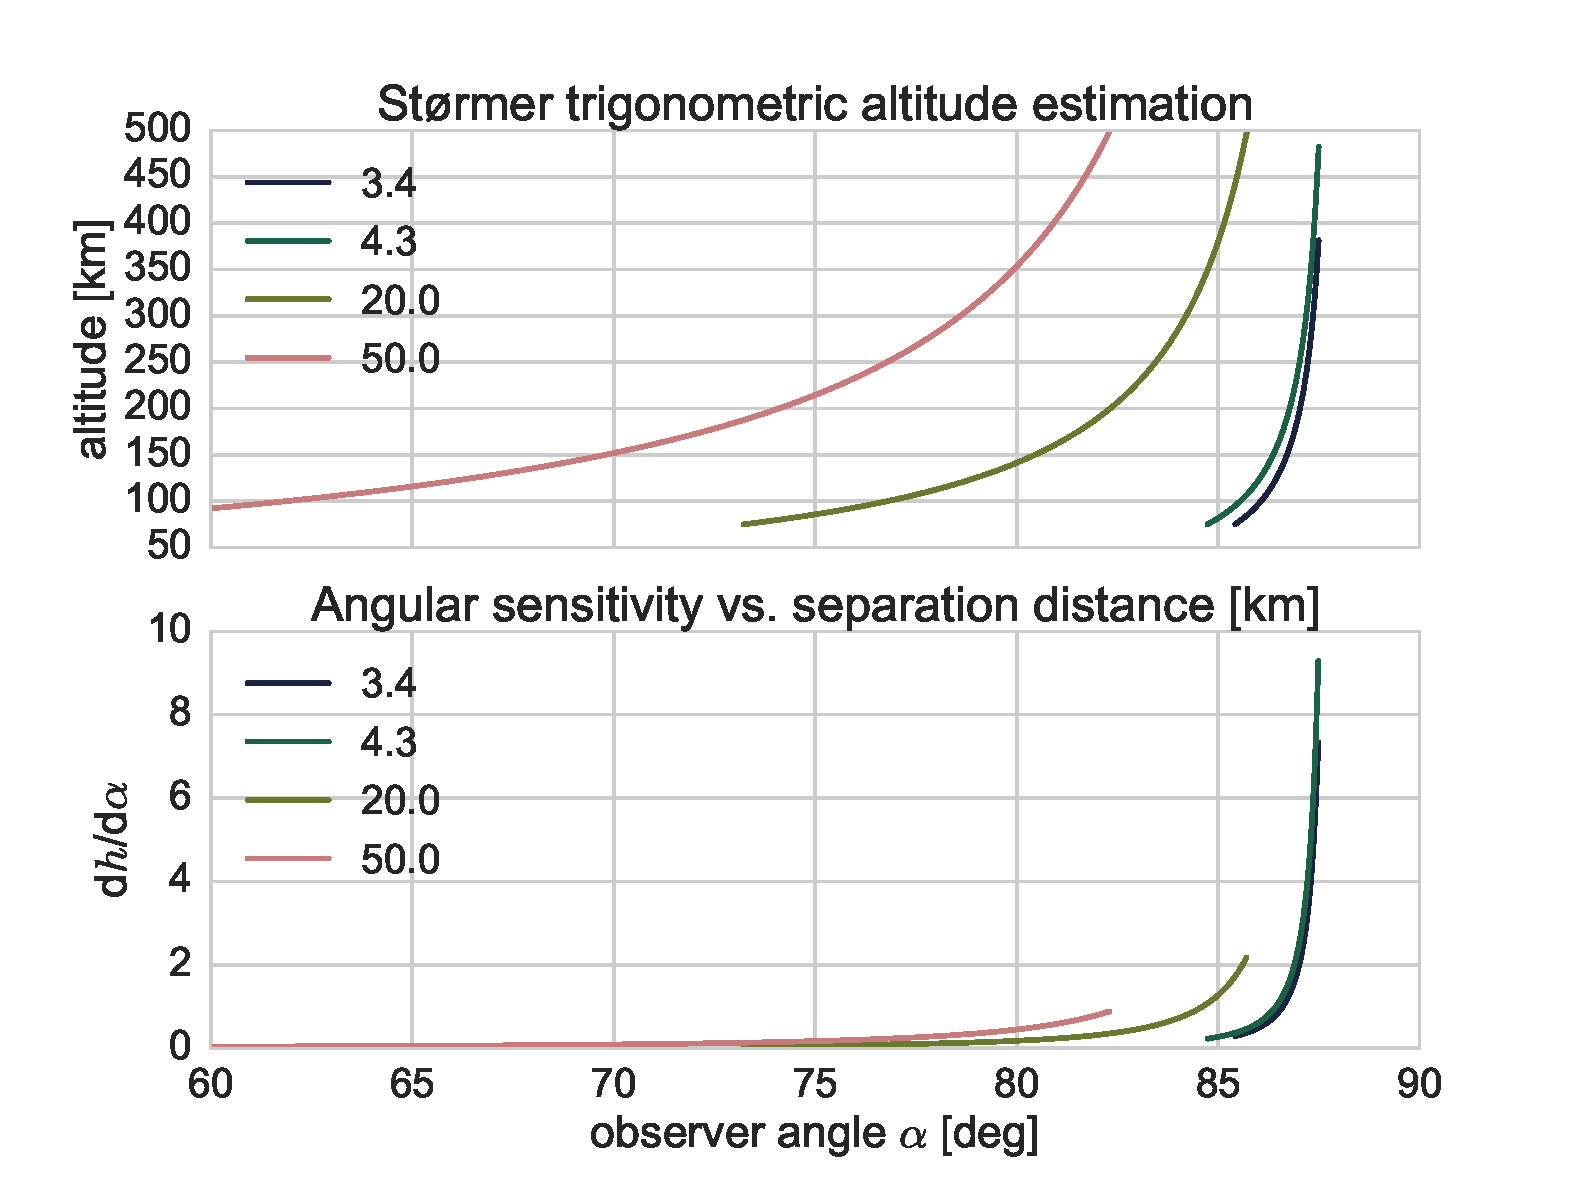
\includegraphics[width=\linewidth]{gfx/stormer_sens}
	\caption{(a) Solutions to \eqref{eq:stormer} for station spacing $x \in \lbrace 3.4, 4.3, 20,50 \rbrace$~km.
		(b) Derivative of \eqref{eq:stormer}, revealing problematic ill-conditioning for narrow-spaced observations.}
	\label{fig:stormersens}
\end{figure}
Considering Størmer's standard $40^\circ$ FOV camera \citep{egeland2013}, film print resolution, optically thin target biasing peak intensity and observer positional uncertainty, it would be difficult to get sufficient accuracy with sub-\unit[5]{km} spaced cameras, from the author's personal experience at these techniques with $9^\circ$ FOV digital cameras.
Timing uncertainty would be significant in Størmer's voice-synchronized \unit[200]{ms} exposure with human auditory-motor reaction time of an excellent athlete under ideal conditions at \unit[82]{ms} mean with \unit[17]{ms} standard deviation \citep{pain2007}.
Consider the profoundly cold outdoor conditions in northern Scandinavia with 1910-vintage clothing, finger slipping on the shutter button, shivering and the like.
It is probable that a mean delay of several hundred milliseconds with large standard deviation might have been the case for an ensemble of freezing students and adult photographers under such trying conditions.
This temporal inaccuracy would not be devastating for inverted-V aurora or other slow to moderate $B_\perp$ apparent speed morphologies.
For the narrow, fast-moving features studied by HiST, such mismatched synchronization would be completely intolerable.


Observational biases, ill-posed/ill-conditioned systems and other inherent remote sensing challenges both instrumental and mathematical, have often been limiting factors in advancing magnetosphere-ionosphere coupling theory.
\textit{In situ} sensing was vital to unlocking physical puzzles at the dawn of the space age and continues to be an essential component to unlocking the secrets of the fine structure of earth's magnetosphere.
Spatiotemporal ambiguities implicit in \textit{in situ} ionosphere and magnetosphere sensing are partially mitigated by close-flying formations of rockets \citep{lynch2012} and satellites \citep{parham2016}.
However, the ability to observe wide swathes of sky at high spatiotemporal resolution is vital to numerous important geospace problems.
An \textit{in situ} platform in motion will always have sampling ambiguities as the structure observed is changing in both space and time as the platform only measures one point in both space and time. 
There is a symbiosis as the \textit{in situ} sensing gives clues as to the particle kinetics responsible for auroral displays, and the ground-based instruments see a swath of sky, using a suitable forward model in the data inversion.

This chapter details the configuration and buildout of the DMC and HiST instruments. 
DMC was a proof-of-concept fielded prototype, observing multiple scales of aurora simultaneously as described in section~\ref{sec:dmc}.
The HiST instrument described in section~\ref{sec:hist} is a full-fledged auroral tomography system, yielding \unit[20]{ms} cadence estimates of auroral precipitation from approximately \unit[50..20000]{eV}, an energy range adequate to characterize Alfvénic aurora and to distinguish alternate particle acceleration mechanisms.
Chapter~\ref{chapter:sim} details the planning and modeling for the optimum \unit[1..10]{km} camera spacing of the HiST system. 
HiST uses robust numerical methods to overcome the ill-posed, ill-conditioned and non-uniqueness problems that frustrated Størmer a century ago.
The purpose of this chapter is to provide historical context of auroral remote sensing leading to HiST, review the state of the art of high-resolution auroral sensors, and describe two specific optical remote sensing systems (DMC/HiST) developed and deployed for the dissertation research.

\section{Auroral Observation Background}\label{sec:obshistory}
The earliest dedicated attempts to photograph aurora in the First Polar Year 1882--1883 was unsuccessful despite \unit[4]{min} exposures \citep{egeland2013}.
The first actual photograph of aurora in 1892 was of too poor quality for quantitative use \citep{egeland2013}.
J. Sýkora's spectrographic plates collected in 1899--1900 were the first quality spectrographic data \citep{chernouss2008}. 
Birkeland tried from 1898--1900 unsuccessfully to simultaneously photograph aurora with two cameras separated by \unit[3.4]{km}, and in 1910 Størmer failed to estimate auroral heights with \unit[4.3]{km} separation \citep{egeland2013} (NB: HiST phase 1 camera separation \unit[3.1]{km}).
Størmer's contributions from 1909 onward resulted in his \unit[0.2]{s} exposure camera carefully constructed to record wavelengths from infrared to UV \citep{stormer1932} becoming the standard camera for IPY 1932.
Hundreds of Størmer's cameras collected a half-million photos, of which tens of thousands were of science-quality \citep{egeland2013}.
Størmer's emphasis on collecting prompt auroral emissions with careful star-based plate scale registration from multiple synchronized cameras separated by about $\unit[20..100]{km}$ may be thought of as direct philosophical ancestors to the HiST system developed during the course of this dissertation.
The problems Størmer's team faced in parsing 500,000 images would have been alleviated by the auroral discriminator developments in chapter~\ref{chapter:discrim}.
Størmer noted that processing one night's image stacks took about a month to process \citep{egeland2013}.

Despite the numerous advances during his long life by himself and others in auroral observations, Størmer passed away before unsolved magnetospheric and ionospheric puzzles began to be resolved via \textit{in situ} sensing of the early satellites.
A 1953 crowdsourcing auroral observation effort using prepaid postcards was plagued by imprecision and inaccuracy of human sighted auroral feature az/el.
It was recognized that replicable, precisely registered, synchronized wide-field optical data was vital to understanding auroral correlation to ionospheric perturbations \citep{birkeland1908,stormer1930,stoffregen1955}.
Leading up to IGY 1957, a network of newly designed ``all-sky'' cameras synchronized with broadband HF receivers were deployed in and near the auroral oval region in Scandinavia.
This effort was designed for better quantification of auroral behavior vs. ionospheric perturbations known then to affect LF-VHF interactions in the ionosphere.
The stations, manufactured in $2\times2$~m huts used the \unit[50]{Hz} power grid via synchronous film-driving motors to ensure sufficiently tight synchronization of the all-sky video. 
A typical setup was \unit[7]{s} uniform exposure, chosen to avoid overexposure while still capturing weak aurora on the \unit[100]{line/mm} film, at \unit[1]{min.} cadence.
Although temporal aliasing was clearly evident in the film strips, this aliasing was a compromise chosen for the great cost of the film required for months to years of observation.
The star registration vital to making altitude estimates of aurora were based on methods by \citet{stormer1930} as updated using current technology.
Deployment of all-sky cameras more extensively about the north and south auroral ovals led quickly to conclusions on the geomagnetic alignment of aurora and the diurnal behavior of the oval versus solar zenith angle \citep{denholm1961}.
The THEMIS all-sky camera network across North America has provided numerous new geophysical insights as used with its satellite--all-sky pairing as well as ISR and rocket experiments \citep{donovan2006}.
The upcoming frame rate improvements via the tREX system \citep{liang2016} will provide a new generation of insights from a medium frame-rate imaging network added to the continent-wide THEMIS ASI network through Canada and Alaska.
HiST phase 2 deployments may include coördinated observations with the tREX/THEMIS network.

A great challenge across STEM disciplines in general and the geosciences specifically is the storage and processing of vast amounts of data over constrained CPU and data bandwidth resources.
The first digital image scanner in 1957 could not hold the 2 bit, $176 \times 176$ pixel image in its \unit[6]{kB} memory, and so the persistence of a scanning oscilloscope phosphor provided the assembled image for human visual appreciation \citep{kirsch1958}.
Over a decade later, the forefront of automated microscope slide processing was an extensively customized computer constructed in a collaboration between multiple US Federal agencies.
This ``Spectre II'' automated cytometry machine was capable of $256 \times 256$ pixel 8-bit resolution, with a single image unable to fit in the \unit[16]{kB} memory \citep{shapiro1969}.
The data reduction employed by Spectre II overcame the issue of a full digitized multi-chromatic microscope slide consuming \unit[62.5]{GB} of storage.
At the time that amount of tape storage would have been over \unit[1200]{km} in length \citep{shapiro1969}, stretching from the earth's surface to over the top of the ionosphere if held vertical.
A contemporary IBM System/360 Model 91 mainframe used by NASA for the Apollo missions had a \unit[16]{MHz} CPU and \unit[2]{MB} of RAM \citep{ibm1967}.
Such computing power was not available in commodity desktop PC form until the late 1980s.
It was not until the 1990s that computer-controlled auroral observation systems with digital storage became common \citep{bjornthesis}.
Computers and hard drives after 2010 (see section~\ref{sec:prochistory}) were finally fast enough to sustain all-night operations from a full-frame, \unit[50]{fps} camera, a key requirement for distinguishing the acceleration mechanism behind plasma turbulence associated with multiple particular auroral forms.

CCD cameras began integration into astronomy in the 1970s \citep{lynds1975} and gradually digital imaging began taking over nearly all aspects of science and personal photography over the next three decades as challenges of imaging efficiency were resolved \citep{monet1993}.
In the past decade, the value of scientific CMOS (sCMOS) cameras has been proven for the high resolution high speed imaging. 
Cooled sCMOS cameras generally exceed the performance of CCD cameras for many applications.
In the most photon-starved regimes, EMCCD cameras reign supreme, as in the HiST system, which like Størmer's system a century before targets prompt emissions from UV to IR.


\section{Dual Multiscale Camera (DMC)}\label{sec:dmc}
Aurora simultaneously evolves on $B_\perp$ scale widths from micro $\sim \unit[10]{m}$ to global $\sim \unit[1000]{km}$.
Within this auroral scale width range there is a continuüm of process scales continually evolving.
Instruments such as THEMIS are designed to observe the auroral oval across the width of North America simultaneously, but at low frame rate with all-sky FOV.
The ASK instrument observes with $3^\circ$ FOV at multiple narrowband wavelengths.
A key novelty of DMC was the simultaneous bandstop prompt emission filtered observation at \unit[33]{ms} cadence at $50^\circ$ and $6^\circ$ FOVs, from a single site.

DMC was constructed in part using cameras obtained for prior experiments such as Mishap and earlier work, funded under NSF EAGER contract \#FA9550-11-1-0356.
Running \$40K each EMCCD and sCMOS cameras designed for clean lab biological operations in short bursts for fluorescence microscopy is quite different than running for 12 hour stretches each night in a shed or box.
The Mishap system \citep{plant2011} deployed in 2011 near Fairbanks, AK experienced significant difficulty with dropped frames and lost timing of frames, using the system timing diagram of Figure~\ref{fig:mishap}.
\begin{sidewaysfigure}
    \includegraphics[page=2,width=0.95\linewidth]{gfx/ProposedTimingSystem}
    \caption{Mishap timing system block diagram form 2010-2011.}\label{fig:mishap}
\end{sidewaysfigure}
Some of these issues were algorithmic, and some were due to the single-core Intel Core 2 Duo E7500 CPU used in Mishap versus the far more powerful quad-core Intel Sandy Bridge i7-2600K CPU used for DMC and the even more powerful quad-core Intel Haswell i7-4790 CPU used for HiST.
As is inherently the case, little insight is gained when comparing different CPU architectures based on clock speed, particularly with on-chip GPUs in processors as modest as the \$25 Raspberry Pi allowing full-screen HD video playback and recording.
Intel Sandy Bridge and newer CPUs made numerous architecture changes \citep{lempel2011}, of which a few are particularly important for high-speed scientific video recording and processing, including:
\begin{enumerate}
    \item elimination of Front Side Bus (bottleneck for RAM and PCI Express cards)
    \item per \#1, bringing the memory controller onto the CPU die
    \item AVX SIMD floating point math-large improvements in automatic vectorization of for loops and other parallelizable problems
\end{enumerate}
The efficiency gains for math operations common to DMC/HiST gave at least a five-fold improvement in processing time.
The same is true for the TRANSCAR energy deposition modeling discussed in section~\ref{sec:fwd}.

The DMC instrument was conceived as a dual-purpose mission:
\begin{enumerate}
    \item test imaging and processing technology essential to HiST functionality
    \item explore correlations between microscale (\unit[0.1..1]{m} width) and mesoscale $\gg \unit[1]{km}$ auroral structure on \unit[20]{ms} timescales
\end{enumerate}
More specifically, DMC mission goals included:
\begin{enumerate}
	\item Two cameras successfully run at full speed for 8 hours, with data rates approaching \unit[500]{MB/s}
	\item Two cameras frame synchronized to better than $\unit[10^{-3}]{s}$
	\item Autonomous system controlled remotely from Internet bandwidth as low as \unit[5]{kB/sec} and latencies $ > \unit[250]{ms}$, using open-source tools
	\item Timing LED device (binary counter) to verify that system doesn't drop or duplicate frames, and that two separate PCs/Cameras are synchronized to specification
	\item Fully automated scheduler (runs without human intervention till hard drives fill)
    \item Sends daily start/stop recording emails, posts logs
	\item online updates with current images posted every $N=60$ seconds
    \item Many debug/disable/error points conveniently located in code
	\item Measured CPU usage during data acquisition $< 10$\%
	\item 16-bit raw grayscale data preserved with lossless compression
	\item actual experiment configuration for each recording stored in XML headers (human-readable) detailing many pertinent camera and algorithm settings, for science and engineering analysis
	\item Programs kept simple enough for research outreach, bringing students quickly to do meaningful work on parts of the program
	\item Data headers human-readable, data format easily accessible via open-source tools.
\end{enumerate}
These mission goals were met and the robustness of the HiST system was greatly improved by having the critical concepts tested in a real field system before deploying the significantly more complicated HiST stations.

\FloatBarrier
\subsection{DMC Build and Deployment}
The benchtop setup of DMC is shown in Figure~\ref{fig:dmcbench}.
\begin{figure}\centering
	\includegraphics[width=\linewidth]{gfx/DMC_bench1}
	\caption{DMC benchtop setup. 
		At left is iXon EMCCD camera with a \unit[17]{mm} lens yielding a $50^\circ$ usable FOV. 
		At right is Neo sCMOS with 140mm lens yielding $6^\circ$ FOV. 
		Both cameras employ BG3 bandstop filters.
		The pan/tilt mount was fixed to be approximately centered on local magnetic zenith, and was constructed by Heitor Murato and Glenn Thayer of BU SIF.}
	\label{fig:dmcbench}
\end{figure}
The iXon camera at left had a usable FOV of $50^\circ \times 50^\circ$ and the Neo camera at right had a usable FOV of $6^\circ \times 8^\circ$.
Both cameras were BG3 filtered as in Figure~\ref{fig:BG3trans} to select prompt emissions as described in section~\ref{sec:physicsemissions}.
It was discovered upon deployment under the dome at Søndrestrøm that the dome was acting as a lens in the near field of the large aperture \unit[140]{mm} Neo lens.
This was confirmed by removing the dome as in Figure~\ref{fig:nodome}, which immediately gave ideal focus.
A flat glass aperture was promptly constructed and installed by Eggert Guðmundsson and crew as depicted in Figure~\ref{fig:dmcflat}.
\begin{figure}\centering
	\includegraphics[width=\linewidth,trim=0 500 0 200,clip]{gfx/DMC_deployed_nodome}
	\caption{DMC installation at Søndrestrøm with dome removed for testing.}
	\label{fig:nodome}
\end{figure}
\begin{figure}\centering
	\includegraphics[width=\linewidth,trim=0 200 0 200,clip]{gfx/DMC-opening}
	\caption{DMC installation at Søndrestrøm with flat glass aperture, giving best possible focus.}
	\label{fig:dmcflat}
\end{figure}
Despite old-age failure and repair of the iXon camera and initial severe issues with the Neo camera driver, the DMC instrument was successful and has supported additional multi-instrument experiments.
DMC remains on site and ready to serve at Søndrestrøm ISR.


\FloatBarrier
\subsection{DMC Data}
DMC quickly yielded interesting data, which has been archived and will be exploited in future work.
Once DMC was working, the focus shifted to HiST build and deployment to take advantage of the same auroral season.
A sample of the novel data coming from DMC is given in Figure~\ref{fig:dmcsplit}.
\begin{figure}
	\includegraphics[width=\linewidth]{gfx/DMC_samples}
	\caption{Example of multiscale insights from DMC on 13 JAN 2013. The upper-left wide FOV images comes from the EMCCD at \unit[33]{fps}, while the \unit[50]{fps} Neo sequence in subpanels 0-4 reveals the fine scale structure invisible to the wide field camera.}
	\label{fig:dmcsplit}
\end{figure}
The splitting arc evolution of \unit[200]{m} width in Figure~\ref{fig:dmcsplit} requires tomographic analysis to quantify the Alfvén wave-driven precipitation causing the arc.
A splitting arc was observed with HiST and PFISR and is analyzed in section~\ref{sec:split}.
Another spitting auroral arc was observed with the cropped image sequence in Figure~\ref{fig:dmcsplit2}.
\begin{sidewaysfigure}
	\includegraphics[width=\linewidth]{gfx/packet}
	\caption{Evolution of splitting arc as observed by Neo sCMOS narrowfield camera. The faint splitting structure would likely be washed out and smeared over by \unit[557.7]{nm} and \unit[630.0]{nm} emissions if not for the bandstop BG3 filter employed.}
	\label{fig:dmcsplit2}
\end{sidewaysfigure}
This fine structure would be completely missed in a widefield camera due to the fine sub-\unit[100]{m} structure.
Finally, a filamentary auroral arc that could come from inverted-V aurora and/or Alfvénic accelerated electrons is shown in Figure~\ref{fig:dmcfil}.
\begin{sidewaysfigure}
	\includegraphics[width=\linewidth]{gfx/filament}
	\caption{Filamentary arc observed by DMC. Determining source acceleration would require a system like HiST to provide differential number flux estimates vs. time.}
	\label{fig:dmcfil}
\end{sidewaysfigure}
Determining source acceleration would require a system like HiST to provide differential number flux estimates vs. time.
These examples are a small taste of the data archived. 
Using the algorithms refined with HiST for joint ISR-optical analysis, future work is anticipated to analyze the single-site cameras data with Søndrestrøm ISR data.
The fast plasma line receiver estimates of electron density will be useful for recent data collected as another data fusion input \citep{vierinen2016}.

As an initial interpretation of these data, it is well established that field-aligned bursts of low energy electron precipitation occur at the edges of dynamic auroral forms. 
ISR measurements have identified anomalous ionospheric turbulence in these regions \citep{akbari2012}. 
\citet{akbari2013} revealed that this edge turbulence appears in thin layers at ranges where the ionospheric density gradients become zero (e.g., the F-region peak, and E-to-F region transition trough). 
Initial DMC observations have revealed a subtle optical signature in this region that appears as a damped outward propagating wave with wavelength $\sim \unit[300]{m}$ in Figure~\ref{fig:dmcsplit2}. Further accumulation of data will establish whether this is a consistent feature at auroral edges; and, finally, systematic comparison with space-borne and ground-based measurements will establish the electrodynamic context of these features and their consequences for communications, navigation, and high-latitude radar discrimination.

%\FloatBarrier
\subsection{Neo Burst Performance Characteristics}
Previous experiments \citep{dahlgren2013} had the operator sitting up all night waiting for aurora to press Record.
This level of human effort is not sustainable in the long term.
Obviously this method misses the build up time to interesting events, and stands a good chance of missing the desired events as well.
Nonetheless, this is how much high-speed auroral observation has taken place prior to about 2010.

For \citet{dahlgren2013} to achieve usable frame rates at full resolution, burst mode was used.
Burst mode uses the on-board camera memory in a short burst, upon which recording stops and the camera RAM is read to the PC RAM over the 3-tap Cameralink interface.
Neither binning or reducing width (width is the 2560 pixel dimension) helps improve frame rates.
Measurements were taken in Table~\ref{tab:neofullburst} at full frame.
\unit[$10^{-5}$]{s} is the minimum possible exposure time of Neo, which is much too short for auroral observations.
\unit[$10^{-3}$]{s} is roughly the minimum useful exposure time for aurora.
\unit[$10^{-2}$]{s} is about the fastest rate the companion iXon would run at. 
At full frame, the iXon can image at \unit[33]{ms} rate.
\begin{table}\centering
	\caption{Andor Neo full-frame burst imaging characteristics}\label{tab:neofullburst}
	\begin{tabular}{p{5em}p{4.5em}p{4.5em}p{5.5em}p{5em}p{5em}}
		\toprule
		Exp. Time (sec.) &  Width (pixels) & Height (pixels) &  Frames / sec &  Max \# of frames &  Max. Burst Time (sec.) \\
		\midrule
		$10^{-5}$ & 2560 & 2160 & 48.95 & 160 & 3.27 \\
		$10^{-3}$ & 2560 & 2160 & 46.68 & 160 & 3.43 \\
		$10^{-2}$ & 2560 & 2160 & 32.87 & 160 & 4.87 \\
		\bottomrule
	\end{tabular}
\end{table}
To optimize viewing area versus frame rate, the data in Table~\ref{tab:neooptburst} was collected.
Neo burst mode performance is optimized by exploiting Neo sCMOS sensor read geometry (center outward)--center on sensor.
\begin{table}\centering
	\caption{Neo burst performance with less than full-height image}\label{tab:neooptburst}
	\begin{tabular}{p{5em}p{4.5em}p{4.5em}p{5.5em}p{5em}p{5em}}
		\toprule
		Exp. Time (sec.) & Width (pixels) & Height (pixels) & Frames / sec & Max \# of frames & Max. Burst Time (sec.) \\
		\midrule
		$10^{-5}$ & 2560 & 1000 & 103.79 & 344 & 3.31\\
		$10^{-5}$ & 2560 & 512 & 197.58 & 667 & 3.38\\
		$10^{-5}$ & 2560 & 256 & 375.64 & 1315 & 3.5\\
		\midrule
		$10^{-3}$ & 2560 & 1000 & 94.12 & 344 & 3.65\\
		$10^{-3}$ & 2560 & 512 & 165.26 & 667 & 4.04\\
		$10^{-3}$ & 2560 & 256 & 273.82 & 1315 & 4.8\\
		\midrule
		$10^{-2}$ & 2560 & 1000 & 67.53 & 344 & 5.09\\
		$10^{-2}$ & 2560 & 512 & 79.87 & 667 & 8.35\\
		$10^{-2}$ & 2560 & 256 & 88.33 & 1315 & $\rightarrow\infty$\\
		\bottomrule
	\end{tabular}
\end{table}
From Table~\ref{tab:neooptburst} and the lens chosen, useful video is not obtained outside of \unit[5]{s} bursts. 
A sustainable mode of operation preserving FOV but sacrificing the excess resolution was required for the DMC mission.

%\FloatBarrier
\subsection{Neo Sustained Recording Performance Characteristics}
The Andor Neo sustained data rates are \textit{substantially} lower than burst mode rates due to the limited 3-tap Cameralink bandwidth.
The Andor Zyla 10-tap Cameralink has significantly higher frame rates than Neo with same sCMOS sensor.
Binning (creating macropixels by grouping adjacent pixels) is the key to sustained useful recording with the Andor Neo.
The maximum sustained frame rate with the Andor Neo using Solis 4.29.30012.0 is given in Table~\ref{tab:neomax}.
The Neo frame rates at 4x4 and 8x8 binning are comparable with the Andor iXon full frame rate.
\begin{table}\centering
	\caption{Neo maximum sustained frame rate with binning}\label{tab:neomax}
	\begin{tabular}{ccc}
		\toprule
		binning & width x height & frames / sec \\
		\midrule
		1x1 & 2560 x 2160 & 20 \\
		2x2 & 1280 x 1080 & 32 \\
		4x4 & 640 x 540 & 54 \\
		8x8 & 320 x 270 & 109 \\
		\bottomrule
	\end{tabular}
\end{table}


%\FloatBarrier
\subsection{Andor Neo DMC Resolution}
The Andor Neo camera has excess resolution for the planned FOV, so the Neo was typically binned 8x8.
An example of the excellent resolution of a splitting auroral arc at these Neo settings is given in Figure~\ref{fig:neosplit}.
\begin{figure}
	\includegraphics[trim=0 0 50 40,clip,width=\linewidth]{gfx/2013-01-13gradient}
	\caption{Splitting arc seen by DMC Neo camera, Jan 13, 2013}\label{fig:neosplit}
\end{figure}
The 3-D view of image intensity seen in the right panel of Figure~\ref{fig:neosplit} shows the fine quality of the focus and resolution with stars appearing as isolated peaks that stay nearly constant from one frame to the next.


\FloatBarrier
\subsection{Andor iXon DMC performance}
The Andor iXon 897 EMCCD (ca. 2003, serial X-1387, EEPROM ver. 6) used for DMC, like the Neo, was a camera reused from earlier projects.
As an EMCCD camera, with the iXon, objects totally invisible to eye \& Fourier analysis on Neo or Zyla can be seen in fine detail with iXon 897 under low-light conditions.
A comparison of important specification between the Neo and iXon is given in Table~\ref{tab:neoixon}.
\begin{table}\centering
	\caption{Comparison of important specification between iXon and Neo}\label{tab:neoixon}
	\begin{tabular}{rcc}
		\toprule
		Item: & iXon 897 & Neo \\
		\midrule
		Photo-electron sensitivity & $<1$ & 2.5 \\
		Pixels (w x h) & 512 x 512 & 2560 x 2160 \\
		Pixel size (microns) & 16 & 6.5 \\
		Sensor size (mm) & 8.2 x 8.2 & 16.6 x 14.0 \\
		Binning & on-chip & software \\
		Binning helps FPS? & YES & NO \\
		Reducing Width helps FPS? & NO & NO  \\
		Reducing Height helps fps, nearest: & bottom of sensor & center of sensor \\
		Minimum air cooling (deg. C) & -40 & -30 \\
		\bottomrule
	\end{tabular}
\end{table}
Images near the magnetic zenith tend to be the brightest by~\eqref{eq:bint}, so wide dynamic range is necessary. 
Because HiST and DMC work several degrees away from magnetic zenith, and faint structures embedded in bright structure is important.
Recent advances in EMCCD technology, after DMC was deployed have taken away the frame rate advantage of the sCMOS cameras for the moment.
HiST is known to have observed faint highly dynamic aurora, just above the noise floor.
These dynamic auroral forms are too faint for the Neo or Zyla sCMOS cameras to detect above the higher noise floor of the sCMOS instrument.
The higher resolution of sCMOS is useful for hyperspectral imagers like LiCHI \citep{goenka2016} that need four simultaneous images.


\section{HiST}\label{sec:hist}
While many of the algorithms and physics details of HiST are described in chapter~\ref{chapter:sim}, we briefly recount key aspects of HiST observations.
Following the successful startup of DMC as described in section~\ref{sec:dmc}, the HiST system final design and build commenced.
The goal of HiST and this dissertation is quantifying fine spatiotemporal auroral drivers, which are themselves of fine spatiotemporal structure.
Extensive forward modeling was carried out to optimize cameras positions as in Figure~\ref{fig:camres} and using theory consistent with optical and ISR observations in \citet{akbari2013}.
As confirmed by DMC experiences and with the new availability of the \unit[50]{fps}-capable iXon Ultra camera, only EMCCD cameras were used for HiST to maximize sensitivity with 16-bit dynamic range.

The initial HiST deployment was carried out by BU postdoc Hanna Dahlgren and then PhD candidates Chhavi Goenka and Hassan Akbari.
The second HiST camera was installed at the MF radar site in an outdoor, non-climate controlled box as shown in Figure~\ref{fig:hst2}.
\begin{figure}\centering
	\includegraphics[width=0.9\linewidth]{gfx/HST1}
	\caption{HiST1 camera installation at the MF radar site in non-climate controlled box.}
	\label{fig:hst2}
\end{figure}
The blue insulation in this box was a help at night but a hindrance during the day, when temperatures rose to the order of $50^\circ$C.
This result led to detailed thermodynamic modeling for the climate control and cabinet system design for HiST Phase 2, as shown in Figure~\ref{fig:hist2cab}.
\begin{figure}
	\includegraphics[width=\linewidth]{gfx/phase2cabinet}
	\caption{HiST Phase 2 cabinet with air conditioning as built in BU SIF.}
	\label{fig:hist2cab}
\end{figure}
This cabinet accommodates two cameras plus GPS and beacon receivers for enhanced data inversion via additional data inputs.
The next section describes the concerns involved with collecting and managing data from three to six cameras at remote unattended installations.

\FloatBarrier
\subsection{HiST Data}
A single camera in the HiST system collects over \unit[100]{GB} per hour, and given the remote unattended deployment of the cameras, substantial data reduction is necessary to avoid on-site human operation.
This reduction algorithm is described in detail in chapter~\ref{chapter:discrim}.
The data surviving this decision is further delineated by passing through the data inversion described in section~\ref{sec:inv}.

When using multiple instruments together to draw observational-based conclusions about the physics expressed by the phenomenon of interest, it is essential to know at least the relative timing error of each instrument. 
The HiST system employs GPSDOs at each camera site to yield timing accuracy $\ll \unit[1]{ms}$. 
Since this is a custom timing system, it is possible that errors in system design or equipment malfunction could cause an unexpected timing error. 
A convenient high temporal resolution test source in the common optical view are low earth orbit (LEO) satellites. 
LEO satellites are also easily visible with ISR in most modes of operation as bright targets > 10 times background.
Thus a tractable time verification can be achieved via an independent source--a geoscience instance of ``trust but verify''.
In particular, the Iridium constellation is a convenient candidate for time synchronization verification due to the large optical cross section and low orbit yielding an optically bright, fast-moving target. 
We must consider errors in SGP4 position propagation and ECI to azimuth and elevation (az/el) coördinate conversion.

The HiST geoscience optical instrument uses cameras including the Andor iXon 897 and iXon 888, with notional parameters described in Table~\ref{tab:ixonrate}. 
\begin{table}\centering
    \caption{Typical dataflow rates for high-speed auroral cameras.}\label{tab:ixonrate}
    \begin{tabular}{lllll}
        \toprule
        Camera & Resolution [pixels] & Bit depth [bits] & frame rate [Hz] & MB/sec \\
        \midrule
        iXon 897 & 512 x 512 & 16 & 50 & 26.2 \\
        iXon 887 & 512 x 512 & 14 & 30 & 15.7 \\
        \bottomrule
    \end{tabular}
\end{table}
It is important for experiment designers to note that camera datasheet frame rates are specified using conditions that are often unrealistic for the extended (many hours) observations typical in auroral observatories. 
By experiments in our lab, a derating of 5\% to 10\% is common for the Andor sCMOS and EMCCD cameras tested, with example sCMOS results shown in Table~\ref{tab:neomax}.
Even at the reduced frame rates in Table~\ref{tab:ixonrate}, imperfections in camera operations (e.g. dropped frames) were commonly observed, as often as multiple times per night.


A hardware monitor of the camera frame acquisition output accounts for any firmware glitches with regard to timing.
The deterministic counter in HiST shown in Figure~\ref{fig:histtime} uses the National Instruments PCIe-6321 with eight timers on an Application Specific Integrated Circuit (ASIC).
\begin{sidewaysfigure}\centering
    \includegraphics[page=1,width=0.95\linewidth]{gfx/ProposedTimingSystem}
    \caption{HiST timing system block diagram.}\label{fig:histtime}
\end{sidewaysfigure}
At the user's option, an additional deterministic timer per site is used to fire the cameras at precise intervals.
For simplicity and especially where the cameras are operated at distinct frame rates with a non-multiple relationship between the cameras, the cameras can be set to free run mode where the absolute time is recovered from the frame acquisition output.
In this manner, any camera with a frame acquisition binary output can be part of the HiST network.
Most scientific cameras with sufficient sensitivity have such an output.

The image collection software and hardware techniques developed in this dissertation are generalizable to any remote imaging system, and were used in developing the HiST Phase 2 instrument.
A map of candidate HiST Phase 2 sites (there will be three sites) is shown in Figure~\ref{fig:hist3}.
\begin{figure}
	\includegraphics[width=\linewidth]{gfx/Optical_Sites3}
	\caption{Candidate sites for three site HiST Phase 2 deployment.}
	\label{fig:hist3}
\end{figure}
Initial processing will be with pairs of cameras, with the eventual goal of integrated three camera plus ISR data inversion.



%\FloatBarrier
\subsection{Poker Flat ISR (PFISR)}\label{sec:fuspfisr}
PFISR produces several low-level data products including the complex analog-to-digital converter voltage samples.
At the time, access to the large files containing low-level PFISR data is by request, with radar data accumulating at $\sim \unit[1.5]{MB/s}$ during a typical experiment.
% data: Apr 14 2013  (468530486 + 224263860 + 224263860 + 187839490) bytes / 729 seconds = 1.516 MByte/sec
Madrigal PFISR high-level data products have integration times $\sim \unit[2]{min}$ versus \unit[10..100]{ms} cadence of the low-level PFISR data.
Long integration time is necessary for plasma parameter estimation since incoherent returns from the ionospheric volume target provide return signals far too weak to characterize from a single pulse.
An autocorrelation function (ACF) is built up from the incoherent electron and ion scatterers over tens of seconds.
Taking the Fourier transform of the ACF the power spectral density (PSD) is obtained, with a notional PSD from a quiet ionosphere shown in Figure~\ref{fig:isrmorph}(a).
An ACF fitting algorithm provides estimates of electron number density, electron and ion temperature and ion velocity.

These plasma parameter estimates break down when turbulent plasma leads to a breakdown in the parameter fitter, which expects PSDs having morphology similar to Figure~\ref{fig:isrmorph}(a).
Strong Langmuir turbulence \citep{akbari2012} leads to ISR spectrum like that depicted in Figure~\ref{fig:isrmorph}(b).
\begin{figure}\centering
    \includegraphics[width=0.8\columnwidth,trim=80 260 100 280,clip]{gfx/isr_thermal}

    \includegraphics[width=0.8\columnwidth,trim=80 260 100 270,clip]{gfx/isr_slt}

    \includegraphics[width=0.8\columnwidth,trim=80 260 100 270,clip]{gfx/isr_streamupflow}
    \caption{(a) Notional PFISR spectrum for quiet ionospheric conditions. 
    	(b) Notional PFISR spectrum under strong Langmuir turbulence. 
    	(c) Notional PFISR spectrum with streaming upflowing plasma.}
    \label{fig:isrmorph}
\end{figure}
Streaming upflows lead to ISR spectrum similar to the depiction in Figure~\ref{fig:isrmorph}(c).
The ISR fitter algorithm used in plasma parameter estimation assumes a single-Maxwellian distribution, which breaks down under turbulent conditions, leading to non-physical plasma parameter estimates.
Alfvénic aurora associated with this Langmuir turbulence leaves fingerprints in the auroral morphology HiST was designed to observe.

The PFISR complex vector $\mathbf{I}+j\mathbf{Q}$ sampled time series is obtained with revisit time as fast as \unit[75]{ms} \citep{akbari2012} for five-beam pattern experiments and may be pushed at least to \unit[19]{ms} \citep{michell2009} for single-beam position experiments.
For future measurements, new ISR plasma line receiver techniques \citep{vierinen2016} reduce plasma line sampling cadence to about \unit[200]{ms}.
Table~\ref{tab:cadence} summarizes the time sampling capability of PFISR.
\begin{table}\centering
    \caption{Instrument sample rates vs. resolution used in experiments.}\label{tab:cadence}
    \begin{tabular}{llll}
        \toprule
        Instrument Measurement Mode & Resolution & Cadence [ms] & Date\\
        \midrule
        PFISR ion line long pulse & five beams    & 75   & 2011-03-01 \\
        PFISR plasma line long pulse & five beams & 6000 &  \\
        Andor Neo sCMOS camera & $1280 \times 1080$  & 20 &  \\
        \midrule
        PFISR ion line long pulse & 23 beams      & 234  & 2013-04-14 \\
        PFISR plasma line long pulse & 23 beams & 14000 &  \\
        Andor iXon EMCCD camera & $512 \times 512$ & 20 & \\
        \bottomrule
    \end{tabular}
\end{table}

Radar receive power for a beam-filling target may be described as
\begin{equation}
%P_r = K\frac{\tau_p P_t}{r^2}G_t G_r n_e \sigma
P_r = (F G_0) P_t L n_e \sigma c \tau \lambda^2 (64 \pi^2 r^2)^{-1} \textrm{[watts]}
\end{equation}
where $P_r$ is power received at the antenna terminals, $F$ is the antenna taper factor accounting for non-boxcar shape of beam, taken as 0.76 in \citet{evans1969}, $G_0$ is boresight antenna gain, $P_t$ is the power transmitted at the antenna terminals, $L$ is radar system losses, $\tau$ is the radar pulse length and $r$ is the one-way slant range to the measured range gate (alternatively called voxel or resolution cell).
The cross section of the beam-filling target is \citep{nicolls2015,evans1969}
\begin{equation}
\sigma = \frac{\sigma_e}{(1+\alpha^2)(1+\frac{T_e}{T_i} + \alpha^2)}
\end{equation}
where $\alpha = 4\pi \lambda_D / \lambda$, the radar cross section of an electron is 
\begin{equation}
\sigma_e = 4 \pi(r_e \sin \psi)^2
\end{equation}
the electron radius is
\begin{equation}
r_e = \frac{e^2}{\varepsilon_0 m_e c^2}
\end{equation}
and $\psi=\pi/2$ for a backscattered electron \citep{evans1969}.
For computing SNR, the noise power is
\begin{equation}
P_n = k_B T_s B
\end{equation}
where $T_s$ is system temperature.
The ISR PSD shape is a function involving many terms, and the reader is referred to \citet{evans1969} equations (18-21) for the specifics.


PFISR ion-line PSD is obtained by taking the Fourier transform of the autocorrelation function.
The ion line spectra are typically observed as two equal-amplitude frequency-smeared impulses symmetric about the radar center frequency.
Typical Doppler bandwidth is less than \unit[25]{kHz} for the \unit[450]{MHz} AMISR.
PFISR plasma-line spectra are shifted several MHz up and down from the radar center frequency, so a slice of the receiver spectrum is extracted where the plasma lines are expected to occur to conserve data and storage resources.
Under quiet and inverted-V auroral conditions, the ISR ion-line spectrum assumptions made by the fitter are fulfilled.
Using assumptions on atmospheric composition (species and density) vs. altitude, an least squares fit of the ion-line PSD is made to estimate the plasma parameters $N_e, T_e, T_i, V_i$.
Further consideration of the fitting of plasma parameters to the ion-line spectrum is given in \citet{swobodathesis}.


A summing-over-altitude technique is useful in both the ion line and plasma line data as a method to draw out weaker coherent returns not otherwise visible.
We integrate $P_r$ in the NEIAL altitude range of roughly \unit[200..400]{km} and plot this integrated measurement as a time series with a representative NEIAL event in Figure~\ref{fig:shedintion}.
\begin{figure}
    \includegraphics[width=0.9\columnwidth]{gfx/2013-04-14T0854/summedAlt2013-04-14T08-54}
    \caption{Receive power of Figure~\ref{fig:20130414T0854a}(e) integrated over \unit[200..350]{km}. 
        Observe turbulence perturbation from approximately 8:54-8:55~UT.}
    \label{fig:shedintion}
\end{figure}
Considering the large amount of raw data collected each day, a method of automated turbulence detection is quite useful, particularly during daylight hours when auroral video is not available.
Cell-median CFAR is the method used in this work.
\citet{schlatter2014} used image processing techniques to further restrict ``matching'' events. 
In contrast, the goal in this work was to achieve high sensitivity and manually filter out spurious events such as satellites.
Most of the time turbulence does not occur, so we can use the median of the last $N$ measurements and set a threshold based on a constant $K$ factor above this rolling median $\widetilde{M}$.
Using Figure~\ref{fig:shedintion} as an example, suppose the rolling median is 50,000.
We can decide detection by
\begin{equation}\label{eq:cfarsum}
S \gtrless K\cdot\widetilde{M}
\end{equation}
based on summed power $S$ vs $K=2.0$ as the threshold factor in this example.


%\section{Digital All-Sky Camera (DASC)}
The DASC instrument has a $360^\circ$ azimuthal view at elevations from horizon to local geographic zenith at $512 \times 512$ pixel resolution. 
When interpreting DASC images, unwarping using \citet{geodata} shows video on the computer screen as it would appear to a human observer looking at the sky, helping eliminate the massive barrel distortion inherent to all-sky images.
On 14 APR 2013, DASC took an image at each of $\lambda \in \lbrace 427.8, 557.5, 630.0 \rbrace$~nm approximately every \unit[13]{s}.
Previous work has combined the three image channels into a pseudo-RGB image, but the issue of temporal aliasing is noted for dispersive auroral events, since each color channel is obtained with about \unit[4]{s} spacing.
%We present the DASC images in three columns by wavelength.
Note that the HiST instrument by design highly attenuates \unit[557.7]{nm} and \unit[630.0]{nm} emissions, while the prompt \unit[427.8]{nm} emission is one of the primary emissions observed by HiST.



\cleardoublepage

\chapter{Dynamic Structured Aurora Discriminator}
\label{chapter:discrim}
\thispagestyle{myheadings}

\graphicspath{{Discrimination/}}

\epigraph{From Spitsbergen, [Svalbard 77$^\circ$ N] in Sept. 1899--Feb. 1900 I observed three intense wavelengths of the Aurora: $\lambda \in \{557.0, 427.6, 391.2\}$~nm. An uninterrupted series of lines was seen between \unit[490]{nm} and \unit[399.5]{nm}.}{\citep{sykora1901}}

Data reduction is integral to geoscience from  Babylonian astronomers through the Mars rovers to facilitate transfer and analysis of data.
Space exploration mission science is constrained by dataflow driven duty cycling limitations on both the space platforms \citep{kurth1979} and the ground stations \citep{deutsch1982}.
Computing advances quantified in section~\ref{sec:prochistory} brought robust computing and storage solutions to the commercial market.
These advances have trickled down to radiation-hard processors, memory and storage sufficient for autonomous driving of Mars rovers \citep{woods2014}.
Novel radio signal processing techniques have enabled rescue of otherwise lost missions and exploration beyond Neptune \citep{deboy2004,haskins2007}.
Much of the data from the 1995 Galileo Jupiter encounter was saved via novel data compression \citep{cheung1996} and fortuitous overprovisioning of storage (\unit[110]{MByte} tape, \unit[192]{kByte} RAM) \citep{marr1994} connected to the late 1970s 1802 CPUs \citep{thomas1980}. 
The lossy compression overcome a 10000:1 reduction in planned downlink data bandwidth, reverting from what was to be a \unit[134.4]{kbps} downlink \citep{layland1990} to \unit[16]{bps} \citep{beyer1996}, allowing Galileo to usefully serve at Jupiter from 1995 to 2003.
The combination of robust embedded computers, storage and wireless connectivity enables a new generation of remote, autonomous geoscience observatories via appropriately designed data reduction algorithms.

Virtually everywhere above ground on earth is covered by ``unlimited'' usage satellite data connectivity at tractable cost.
Iridium unlimited data usage is currently \$125/month\footnote{Pricing for Iridium GO! via \url{http://www.bluecosmo.com/iridium-go/rate-plans}} at \unit[2.4]{kbps}, with future speeds up to \unit[128]{kbps} and essentially global coverage.
Covering the northern auroral oval and beyond, unlimited usage satellite data from Globalstar is currently \$150/month at \unit[9.6]{kbps}, with future speeds up to \unit[256]{kbps} \citep{globalstar2015}.
The Globalstar data rate with coverage area shown in Figure~\ref{fig:globalstar} is similar to that experienced with the DMC instrument in section~\ref{sec:dmc}.
\begin{figure}
    \includegraphics[width=\linewidth]{gfx/voice-coverage_map_lg_w_homezone_oct31_14}
    \caption{Current Globalstar satellite data coverage area in yellow and gray.}\label{fig:globalstar}
\end{figure}
Terrestrial mobile data networks generally have higher data bandwidth than satellite.
Due to petrochemical extraction and other human activity, 4G networks are extending across the auroral zone.
Even the slopes and summit of Mt.\ Everest have 4G cellular service \citep{oberhaus2016}. 
%since 2011, with Everest base camp having satellite connectivity since 1996.
Cubesats are forming networks to relay data on orbit for terrestrial downlink \citep{parham2016}.
Commercial magnetometers aboard he Iridium 66~satellite constellation have been turned into the AMPERE observatory \citep{waters2001}.
AMPERE creates a global current map relevant to auroral precipitation using geomagnetic spherical harmonic analysis introduced by \citet{gauss1839}.

As a practical matter for geoscience imaging systems, data rates less than about \unit[4.8]{kbps} are useful for system control and low resolution preview data, while data rates above \unit[9.6]{kbps} become practical for curated retrieval of limited data sets.
Historically this has meant taking a picture of the aurora perhaps once per minute since there was no means of storing or transmitting vast amounts of high speed video--a problem from 1900 through the developments of this chapter started in 2012.
The experience with the DMC instrument in Greenland and isolated deployments for the HiST system using 4G wireless data have shown the utility of automated data reduction algorithms for auroral research.
With the algorithms developed in this chapter, auroral and geoscience radar researchers can record high speed data and store/download interesting segments of data remotely.

For geospace data in general and in particular for auroral video observatories, significant portions of data collected will be of little value relative to the cost of transporting the data.
Multiple generations of geospace satellites have duty cycled observations to conserve power, storage, and downlink bandwidth.
While miniature instrument technologies and streaming data bandwidths have  advanced to the point where cameras and radars covering the entire MF/HF band fit into a 3U Cubesat \citep{knapp2016}, data downlinks are strained by the amount of data collected.
Most contemporary high speed auroral imaging systems are severely limited by duty cycle to avoid overflowing their on-site data storage \citep{fukuda2016}.

Distributed geospace sensors, particularly dense arrays with dozens or hundreds of nodes \citep{pankratius2014}, can benefit from on-site data reduction.
Even though 4G connectivity in the northern auroral oval (approximately $60^\circ$N to $70^\circ$N) continues to expand, the coverage is generally spotty due to terrain and great inter-tower distances.
Figure~\ref{fig:gci} is an example of the spotty coverage endemic to rural areas due to low tower density and vast distances with terrain.
\begin{figure}\centering
	\includegraphics[width=\linewidth,trim=0 45 0 0,clip]{gfx/gci4g-pfrr}
	\caption{GCI wireless data coverage near Poker Flat Research Range. Map is roughly \unit[30]{km} in vertical extent.}\label{fig:gci}
\end{figure}
Weak wireless signals directly imply reduced data speed via the Shannon-Hartley theorem \citep{nyquist1924,hartley1928,shannon1948a,shannon1948b,lee1990}
\begin{equation}\label{eq:shannon}
C = B \log_2\left(1+\frac{S}{N}\right)
\end{equation}
where $C$ is the channel capacity in bits/s, $B$ is the channel bandwidth in Hz, $N$ is the noise power in $B$ and $S$ is the signal power. 
Software defined radio sensors for HF, GPS and other radar applications generate up to the order of a terabyte of data per day, while EMCCD and sCMOS cameras used for auroral and airglow observations generate several terabytes per night \citep{hirsch2016}.
Assuming unlimited data plans (2016 prices $\sim$ \$200/month) and future \unit[1]{Gbps} radio data bandwidth, the avalanche of data from hundreds of sensors must be sifted through at some point in the system lifetime.

Where sufficient local computing power (both CPU and watts) exists, it is typically advantageous to reduce the data on-site before transmitting to a central repository.
For those situations where it is desirable to retain all data to allow for discovery of an unknown, as yet uncharacterized phenomenon, data reduction techniques are still essential for tagging known event types.
In general, remote geoscience observatories require on-site and/or fog computing due to constrained storage and data bandwidth to the outside world.
The problem of high-bandwidth sensors with constrained connections is common in remote sensing system, including smart transportation \citep{hou2016}.
A common sparse messaging format allows telling groups of sensors to store segments of high resolution data without processing the data at each and every node all the time.
An HDF5 format file with the nightly triggering record from a high-power sensor node is less than \unit[25]{kB} for a 12 hour period, a size readily relayed over a \unit[1.2]{kbps} radio link.
Integrated radio modules with antennas cost about \$50 and use world-wide license-free frequencies near \unit[900]{MHz} with approximately \unit[1]{km} range between nodes.
By \eqref{eq:shannon}, using larger directional antennas allows longer range or higher data rates.
An example of the utility of such a system is a dense network of high speed magnetometers with kilometer grid spacing \citep{raeder2016}, where to conserve solar-charged batteries, recording and/or relaying of data only occurs on all nodes during auroral events.

A large subclass of geospace instruments are designed to observe infrequent, irregularly occurring events.
Instruments designed to capture only the strongest events (typically making a sensor cheaper) will cost much more in terms of lost sensing opportunities and wasted energy and exergy.
Instruments are often a bit overdesigned in terms of sensitivity and dynamic range to allow for discovery of new phenomena.
The slight Arecibo overdesign for plasma characterization \citep{farley2012} allowed the radar to receive gyro-line plasma emissions. 
Arecibo's increased SNR is also used for planetary body characterization and asteroid imaging to complement facilities such as the shorter wavelength Goldstone Radar \citep{slade2011}.
Higher instrument sensitivity may bring new discoveries via newly seen weak signals, which need to be sifted through for events of interest.

For auroral targets specifically, several attributes of the targets have been exploited.
\citet{rao2014} used RGB-transformed color as an essential component of auroral detection at multiple stages.
For reasons stated in chapter~\ref{chapter:sim}, only grayscale video is available from HiST.
Several machine learning approaches have been used for slow-acquiring all-sky cameras that collect as many frames in a year as HiST does for each camera per night \citep{mikka2005}.
Decomposition methods have been applied to high-SNR video as part of an effort to create a search engine for auroral forms \citep{mikka2002}.
These methods are not suitable for the high speed auroral video generated by the DMC and HiST instruments.

DMC and HiST need a fast auroral detection algorithm to wade through terabytes of data per camera per night. 
Unlike previous efforts, the dynamic structured aurora discriminator (DSAD) algorithm does not necessarily need to make a final classification of auroral type, particularly when used with the HiST inversion algorithm described in chapter~\ref{chapter:sim}.
The DSAD task of interest is detecting fine spatiotemporal auroral features, which have distinct characteristics that are exploited via a collective behavior algorithm developed for this thesis.
A modified version of the DSAD algorithm has been extended to passive ionospheric radar, described in appendix~\ref{chapter:passive}.
Another modified DSAD application is demonstrated for the HF top-sounding radar MARSIS exploring the Martian ionosphere in appendix~\ref{chapter:marsis}.

\section{Auroral Data Processing Background}\label{sec:prochistory}
Quantitative auroral observations rely on large datasets collected at multiple locations over an extended period of time (see section~\ref{sec:obshistory}).
A general algorithm for the processing of auroral data is depicted in Figure~\ref{fig:genalgo}.
\begin{figure}\centering 
    %the \par is necessary after each text to make the \baselineskip take effect
    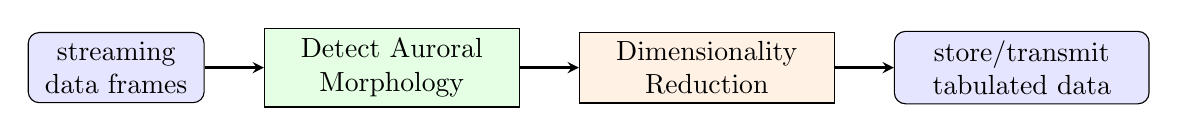
\begin{tikzpicture}[node distance=1.5cm, auto]
    
    \node (in) [startstop,text width=2cm] {streaming data frames \par};
    
    \node (detect) [compute, right of=in,text width=3cm,xshift=2cm] { Detect Auroral Morphology \par };
    
    \node (reduce) [process, right of=detect, text width=3cm,xshift=2.5cm] { Dimensionality Reduction \par };

	\node (store) [startstop, right of=reduce,text width=3cm,xshift=2.5cm] { store/transmit tabulated data \par};
    
    \draw[arrow] (in) -- (detect);
    \draw[arrow] (detect) -- (reduce);
    \draw[arrow] (reduce) -- (store);

    
    \end{tikzpicture}
    
    \caption{Block diagram of DSAD algorithm.}
    \label{fig:genalgo}
\end{figure}
%Tables of auroral activity versus time and location were extensively compiled in the 1700s (see section~\ref{sec:historyaurora}), a simple but highly lossy form of data reduction.
The technology necessary for quantitative spatiotemporal observations on sub-second timescales necessary for understanding structured aurora evolved throughout the twentieth century via several technological advances:
\begin{enumerate}
    \item quality spectrum resolution: \citep{sykora1901} high resolution, sensitive auroral spectrum obtained with several hour exposures % to day-long
    \item stable fast optics: \citep{stormer1932} auroral images capturing from UV to IR with half-second exposure, with hundreds of cameras manufactured and globally distributed for IPY 1932 (see section~\ref{sec:obshistory}).
    \item stable stopband filters: \citep{rayleigh1924} using repeatable Kodak Wratten filter arrangement allowed blocking undesired emissions while maximizing observed brightness, in a replicable, global transportable system.
    \item fast energy spectrum of precipitating particles: \citep{sharp1965} \unit[8]{ms} cadence broadband differential number flux, revealed fine spatiotemporal structure and that electrons were responsible for structured aurora
\end{enumerate} 
Several more developments enabling digital computer processing of video were necessary to enable the millisecond timescale auroral observations of the twenty-first century:
\begin{enumerate}[resume]
    \item digital cameras: CCD technology that came to market in the early 1970s and subsequent market availability of intensified CCD (iCCD), sCMOS, and EMCCD imagers rugged and inexpensive enough for global shipment and reuse by the early 2000s.
    \item large, fast, durable portable storage media: by 2008 beginning to be adequate for storing one night's data and by 2009 \unit[2]{TB} HDDs available for \$300 \citep{first2tb} capable of two nights' data.
\end{enumerate}
Corporate termination of scientific film production in the mid-1990s \citep{malin1993} combined with the rise of wider dynamic range, high sensitivity digital scientific cameras accelerated the switchover from analog to digital imaging.
ISR also benefited from the advances in computer technology to process 4096 antenna elements worth of reduced streaming data.
High-power microwave modules and associated technology for electrically steerable phased array radar \citep{valentic2013} and broadband software defined radio \citep{vierinen2016} are additional vital developments necessary for quantitative analysis of NEIALs vis-à-vis Alfvénic aurora.

\subsection{Computing Hardware Relevant to Auroral Data Processing}\label{sec:currentpc}
%  = 1.27 TB / 12 hour night
Since each EMCCD camera used in HiST generates on the order of
\begin{equation}\label{eq:mbsec}
    \unit[512^2]{pixels} \times \unit[2]{bytes/pixel} \times \unit[56]{frames/s} \sim \unit[29.4]{MB/s} 
\end{equation}
\begin{equation}
     \unit[(29.4\times 3600)]{frames/hour} \times \unit[10]{hours} \sim \unit[1.1]{TB/night}
\end{equation}
an internal HDD with at least \unit[1.5]{TB} of storage is necessary to avoid excessive fragmentation upon writing each night's data.
Fragmentation is relatively benign on SSD but for HDD the large additional mechanical seek time from fragmentation can cause greater than 90\% reduction in read/write rate, which is problematic for auroral video.
Empirically we have found that keeping the HDD with at least 5\% free space using exFAT formatting \citep{munegowda2014exfat} has avoided write speed problems due to fragmentation.
By \eqref{eq:mbsec} and lab experiments conducted during lab verification of DMC and HiST phase 1, the HDD should have at least \unit[75]{MB/s} sustained write speed, giving margin for nonidealities and congestion involved in sustained sequential writes to avoid overflowing the RAM buffer and thereby losing data.
Sustained HDD write speed specifications may be actually given as an average or N\textsuperscript{th} percentile, and also depends on format and operating system overhead, so at least a cursory lab verification before buying several HDD is well-justified.
An example of lesser real-world performance versus spec sheet was given by \citet{hddrealworld}, in accord with experience in DMC lab verification.
Real USB~2.0 HDD are limited to about \unit[40]{MB/s} sustained sequential write speed.
Putting the same modern HDD into a USB~3.0 enclosure will typically show HDD write speed $>\unit[100]{MB/s}$.
When using USB~3.0, magnetic HDD sequential write speed are primarily limited by the drive magnetics due to the USB~3.0 theoretical maximum \unit[5.0]{Gbps} throughput versus USB~2.0 theoretical maximum \unit[480]{Mbps} throughput.
Not all USB~3.0 chipsets perform to theoretical maximum, and constraints of the motherboard buses can be significant.
When planning a high bandwidth optical system using high-resolution sCMOS cameras, lab tests are essential to determining actual field-realizable parameters as demonstrated in Table~\ref{tab:neomax}.

By 2009, consumer desktop PC CPUs were fast enough with internal HDD storage sufficient for one night's data.
However, for practical long term archiving of data, external USB~3.0 HDD \citep{firstusb3hdd} and USB~3.0 certified motherboards \citep{firstusb3pc} were not commonly available until 2010.
This was fortuitous timing for the planning and development of the DMC system, a technology testbed for HiST.
High-end consumer motherboards of 2010 commonly supported at least \unit[16]{GB} of RAM and had the multiple PCI Express slots necessary to run the EMCCD and sCMOS cameras at full frame rate.
\unit[16]{GB} of RAM was sufficient for a circular buffer adequate to withstand HDD write hiccups.
Thus, the computer technology needed to accomplish HiST was first commercially available in 2010.

Keeping all the data, even just the ``good'' data can become costly, a problem universal in auroral observations from 1900 onward.
Figure~\ref{fig:hddcost} shows the logarithmic progress of HDD cost/GB.
\begin{figure}
    \includegraphics[width=\linewidth]{gfx/hdd-cost-per-gigabyte-large}
    \caption{HDD cost/GB vs. year \citep{hddcost}. \unit[1]{TB} HDD introduced 2007 \citep{first1tb}, \unit[1.5]{TB} introduced 2008 \citep{firsthdd}.}\label{fig:hddcost}
\end{figure}
HDD durability has been maintained despite the cost drop and storage increase  , such that a typical portable USB HDD has a 3-5 year warranty. 
Test results by global leaders in HDD storage have repeatedly shown that consumer HDDs are sufficiently robust for many geoscience storage tasks, as long as proper backup procedures are in place.
Figure~\ref{fig:hddreliability} shows recent HDD reliability under rigorous real-world controlled testing.
\begin{figure}
    \includegraphics[width=\linewidth]{gfx/drive-stats-2016-q1-failure-by-mfg}
    \caption{Failure rate of large number of continuously used HDD \citep{backblaze2016}.}\label{fig:hddreliability}
\end{figure}
HDD data loss by UAF collaborators has been experienced on some dates HiST was used.
When interesting auroral video is identified, it is copied to multiple drives and when possible the very best snippets are prompted uploaded to Google Drive and other robust cloud storage to help avoid complete data loss.
Figure~\ref{fig:tapeloss} shows file loss experienced on a very large data storage project.
This loss was experienced on high reliability tape drives in a carefully monitored system, and so might be thought of as an example of a practical upper bound on data reliability.
\begin{figure}
    \includegraphics[width=\linewidth]{gfx/tapeloss}
    \caption{Data loss experienced by CERN high reliability storage system \citep{cancio2015}.}\label{fig:tapeloss}
\end{figure}

An example of a leading enterprise HDD \citep{first10tb} is the \unit[10]{TB} Seagate Ironwolf ST10000NE0004 \citep{ironwolf} currently available for \$479.
A five year warranty with \unit[300]{TB/year} write rating exceeds the expected \unit[265]{TB/year} raw data written from a single camera.
As an enterprise HDD, the Ironwolf full-time $24\times7$ failure rate is 0.73\%, substantially better than the consumer HDD of Figure~\ref{fig:hddreliability}.
The sustained data rate specification of \unit[214]{MB/s} is better than some solid state drives (SSD), and is fast enough to handle $2\times2$ binned Andor Neo sCMOS $2560\times2160$ pixel video streaming.
The HDD buffer memory of \unit[256]{MB} is enough to hold
\begin{equation}
256 / \unit[512^2]{pixels} \times \unit[2]{bytes/pixel} \times \unit[56]{frames/s} = \unit[8.7]{s}
\end{equation}
of full frame-rate EMCCD video, a generous margin for operating system hiccups or isolated fragmentation, considering that the HiST program has a RAM pseudocircular buffer as well.

Banks of USB~3.0 external HDD are used for on-site archiving, and may be swapped yearly or as desired if too much data to send over the broadband cellular modem exists.
Assuming Alfvénic or other interesting aurora occurs no more than 10\% of recorded hours, four USB~3.0 HDD at $< \$2000$ total cost are sufficient to store a year's worth of interesting auroral data.
Sections~\ref{sec:obshistory} and~\ref{sec:prochistory} detail the problems solved by industrial technological process and aeronomers to make the next decade one of significant progress in synchronized auroral/ionospheric observations.
Section~\ref{sec:discalgo} describes the DSAD algorithm necessary to process manageable amounts of data, as the full HiST inversion process of chapter~\ref{chapter:sim} is too time-consuming to run on every single frame of data using a single desktop PC. 
If large amounts of data (too much for a single desktop PC) were deemed interesting, computing clusters such as SCC would be very amenable to parallel processing the HiST data inversion.

\section{Dynamic Structured Aurora Discriminator Algorithm}\label{sec:discalgo}

Alfvénic auroral morphology includes:
\begin{enumerate}
    \item laterally splitting arcs
    \item thin, rapidly laterally moving auroral arcs
    \item flaming aurora consistent with DAW from \unit[100]{eV}..\unit[10]{keV} electron precipitation
\end{enumerate}
The DSAD algorithm was needed for the HiST system in order to avoid having to manually wade through the 90+\% of video without the fine $B_\perp$ spatiotemporal dynamics corresponding to DAW particle acceleration.
Section~\ref{sec:cvmot} gives background and motivation for the DSAD algorithm developed during the dissertation work for the DMC and HiST systems.
Subsequent sections describe the components of the DSAD algorithm depicted in Figure~\ref{fig:blockcv}.


\subsection{Machine Vision Applied to Auroral Video}\label{sec:cvmot}
The design of geoscience remote sensing instruments, whether ground-based, space-based or somewhere in-between generally is designed around the amount of dataflow from the instrument to the researcher.
Geoscience instrument dataflow may be streamed over the Internet or via a radio transceiver.
Instruments more remotely located are more likely to cache data on-site, like a satellite ejecting a film canister \citep{nageswararao2009} or human doing a yearly swap of an SD card in a remotely-sited magnetometer instrument.
Some geoscience instrument data may never be transmitted due to to transmission or storage media errors.
Other systems by design use FIFO/circular buffers, decimation and other techniques to discard uninteresting data or data of excess fidelity.
Ultimately there is a dataflow constraint that helps drive the overall instrument design.

At present, computer technology is capable of storing and online processing of the full speed datastream of geoscience instruments that computers of a decade ago could only process in short bursts, for example the analysis in \citet{dahlgren2013}.
Computer vision techniques adequate for detecting Alfvénic aurora have been implemented for the DMC and HiST systems and are well within the capability of a commodity PC used for camera data acquisition.
As technology improves in high-speed science-grade cameras (so denoted for reasons including repeatability of absolutely scaled intensity) and multi-core CPUs, the ability to conduct extended ionospheric observations at time sampling rates approaching the limits of ground-observable SNR-limited physics has at last become feasible \citep{hirsch2016}.
%Portable USB 3 hard drives have grown adequate to capture 200~GB/hour from 50~fps Electron Multiplying Charge Coupled Device (EMCCD) cameras.
%A season's worth of aurora can be stored in 8~terabyte USB~3 hard drives at each camera site, assuming there is aurora of interest for 5\% of the dark hours.
Autonomous machine vision algorithms allow storing only auroral video of the desired morphology (e.g. thin discrete arcs), saving hard drive space and human review time via automatic upload of interesting video snippets to a public repository for prompt access.
The HDF5 \citep{hdf5} auroral image stacks are uploaded to Zenodo \citep{zenodo} for permanent public archiving.
Modern processing algorithms such as \citet{isrutils} allow rapid loading and processing of the large ISR raw data files.

Most geoscience dataflows employ data reduction in the course of estimating an unobservable science quantity.
For example, a project like Aurorasaurus.org \citep{macdonald2015} must reduce raw human input via a variety of established methods to winnow out useful tweets from the flood of tweets mentioning terms that possibly involve geophysical aurora displays in sight of the Twitter user.
Rarely observed events such as auroral beading have had some of the best data collected \citep{aurorasaurus-bead} from the Aurorasaurus project.
Another example of an aurora-associated phenomenon requiring long-term persistent observation are the occasionally human-reported sounds associated with aurora that were long thought debunked--until several years of persistent observation paid off with observations leading to estimates of an acoustically-plausible source altitude time-correlated with auroral dynamics \citep{audio2016}.

One of the factors delaying discovery of new phenomena and revisiting old phenomena to enhance or replace explanations is the typical need for the human observation team to sit in a shed or car watching over the expensive equipment in a several day or week campaign.
Having designated days or weeks where all available instruments are turned on is beneficial for new insights.
It would be even more advantageous for new discoveries and statistics to simply have all the instruments on all the time.
A few factors working against long-term persistent unattended ground-based observatories include:
\begin{enumerate}
    \item Too expensive per-site instrumentation (fear of theft)
    \item Too much data to store
    \item Software not robust enough for unattended operation
\end{enumerate}
The ``expensive per-site equipment'' issue is being solved by a new wave of experimental designers including the author using advances in computer, open source, and software-defined instrument technology.
The ``too much data'' and ``software not robust'' problems are addressed in the dissertation work.

The \unit[10]{TB} internal HDD available today are enough for several nights of data from a typical EMCCD camera in increasing use for quantitative auroral observation.
This helps avoid certain improvised solutions for collecting data such as:
\begin{itemize}
    \item reduced frame rate
    \item human on-site or remotely watching video to press ``record''
    \item collecting periodic bursts of data
\end{itemize}
Those improvised workarounds result in substantial loss of data and increased effort to manually peruse what data is collected.
By simply collecting all the video each night of auroral observation, as long as we can process the video via software fast enough during the day, we will clear out the unwanted data and copy out only the ``good'' data.
By not needing to do on-line, real-time filtering of the video stream, we can employ much more sophisticated algorithms without the need to worry about multi-core processing, RAM capacity, and the like.
This improves overall robustness of the data collection and significantly reduces difficulty of programming.

Assuming the camera manufacturer has done an appropriate design and specification verification, writing a program to simply start and stop the camera at dusk and dawn, saving all data to disk should be straightforward.
One may rely on operating system disk buffering to handle slight hiccups due to hard drive seeks.
Intuitively it is appropriate to use a second hard drive dedicated to data for writing, not sharing the same hard drive as the operating system--even if the hard drive is solid state due to seek time and IOPs limitations of the OS-hosting HDD.

Previous work in the area of auroral detection has included static brightness thresholding, dynamic histogram thresholding akin to Otsu's Method \citep{otsu1979}, and skeletonizing \citep{lam1992,saeed2010}.
The auroral forms of interest for this manuscript are those driven by DAW.
An auroral classifier that distinguishes between thin aurora forms as in Figure~\ref{fig:cartoonmorph} vs. diffuse auroral forms is suitable for this task. 
The data inversion algorithm of chapter~\ref{chapter:sim} completes the discrimination between inverted-V driven aurora vs. two-stream upflow vs. Alfvén aurora.
Note that the auroral forms of interest may be quite faint, perhaps with brightness near or below the camera noise level.
The algorithm described in this section detects interesting auroral forms with such low SNR that they are not immediately obvious to humans watching the video.
The false positive rate is low enough so as not to be burdensome to the system operators.

For Alfvénic auroral arcs viewed in an image stack with axes (x,y), there is generally observed motion of the arc along $B_\perp$, such that for pixel intensity $I$
\begin{eqnarray}\label{eq:alwaysmoving}
C_x > \left|\frac{\partial I}{\partial x}\right| & \gg & 0 \\
C_y > \left|\frac{\partial I}{\partial y}\right| & \gg & 0 \nonumber
\end{eqnarray}
and let
\begin{equation}
 C = C_x \equiv C_y.
\end{equation}
$C$ is chosen using a median constant false alarm rate (CFAR) method, adapting to spatially discrete, noisy point sources such as stars.
\eqref{eq:alwaysmoving} implies that
\begin{equation}\label{eq:changingI}
\frac{\partial I}{\partial t} \neq 0
\end{equation}
due to the optically thin nature of aurora expressed in \eqref{eq:bint}.
\eqref{eq:changingI} violates the data conservation constraint employed with classic optical flow techniques.
This violation will have a spatially coherent behavior materially different than the environmental and sensor noise--a factor to exploit in automated auroral detection \citep{blixt2006}.
Salient characteristics of the interesting auroral forms include:
\begin{enumerate}
    \item collective behavior: the arc might deform, split, or translate but with spatial cohesion
    \item discernible width: (maximum to 10\% brightness) of about 100..1000~m 
    \item spatially smooth: diffusion implies there is no spatial ``popcorning'' or highly discrete illumination like stars
\end{enumerate}

\FloatBarrier
\subsection{Loading video data}\label{sec:load}
We process the whole night of auroral image data offline.
As described in section~\ref{sec:currentpc}, commodity computer hardware currently available allows recording all night.
On-line processing will necessarily be time-constrained, and if some unexpected event occurs (e.g. meteor, vehicle reentry) the possibly unique data would be lost as the discrimination algorithm is not tuned for such an event.

For reduced processing time, one can choose to sample every N\textsuperscript{th} frame set.
Deciding which interval to sample at is driven by the need to sample the entire night's data and extract interesting frames before it's time to record again for the next night.
Although DAW events evolve on sub-second time scales, there are generally several DAW sub-events happening in parallel and serially over 5..\unit[15]{s} intervals, with several such groups of events occurring within 1..\unit[5]{min.}
The bounds on discrimination algorithm data loading cadence $T_L$ in seconds is thus bounded by
\begin{equation}\label{eq:loadint}
T_0 < T_L < T_1.
\end{equation}
Empirically, an Intel i7 Ivy Bridge CPU yields $N \gtrsim 20$ and with camera kinetic rate $T_K=\unit[20]{ms}$, $T_0 \sim \unit[400]{ms}$.
Given typical event duration $\unit[5]{s} \lesssim T_E \lesssim \unit[15]{s}$, $T_1 \sim \unit[2]{s}$.
Thus \eqref{eq:loadint} becomes
\begin{equation}\label{eq:actload}
0.4 < T_L < 2.
\end{equation}
As computer hardware capability increases with future CPU generations, $T_0$ becomes smaller and/or more advanced discrimination algorithms may be employed.

The images are stored in a raw binary stream containing a fixed-length footer containing a sequence number and other user-chosen per-frame metadata.
DMC and HiST phase 1 used a four byte footer for this purpose.
For simplicity, the experiment configuration is stored in a standard XML file.
The raw binary file will be more than \unit[1]{TB} in size for a whole night recording, so for ease of download and user experience auroral events of interest are repacked into an losslessly compressed HDF5 format file.
The HDF5 file is chunked, one image per chunk for fastest reading, combined with metadata like the format used by the Madrigal geospace data repository \citep{madrigal} and uploaded to Zenodo.

Auroral image histograms are not adequate to discriminate on alone since they do not contain sufficient information about the morphology. 
The ground-observed brightness of aurora is highly dependent upon viewing angle and the arrangement of the aurora along a particular viewing angle as described by~\eqref{eq:bint}.
An example auroral histogram on a clear viewing night with a few bright stars and a discrete arc away from magnetic zenith is shown in Figure~\ref{fig:diffimhist}.
\begin{figure}\centering
    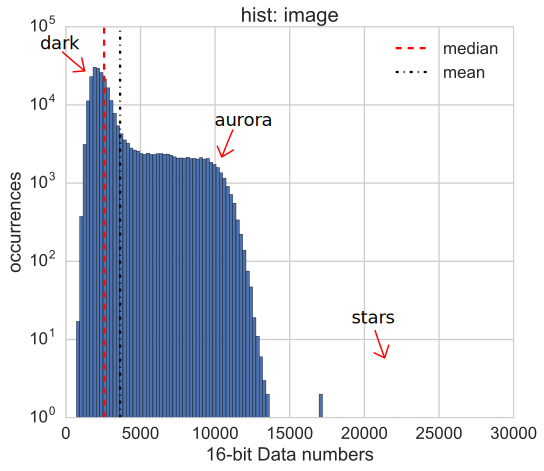
\includegraphics[width=0.7\linewidth]{gfx/diffuse-imhist}
    \caption{Histogram of discrete arc away from magnetic zenith.}\label{fig:diffimhist}
\end{figure}
Due to photon-stared low auroral video SNR, there is no clear separation between auroral intensity values and background noise, thus even adaptive intensity threshold algorithms fail.

\FloatBarrier
\subsection{Image Noise Filtering}\label{sec:filtnoise}
Noise reduction is a common preprocessing step, particularly in auroral video where SNR is often low and the target is smooth as a result of diffusion of the particle stream scale for $\unit[100]{m} > B_\perp > \unit[10]{m}$ in the ionosphere.
The 2-D Wiener filter is often chosen for auroral video noise reduction as the Wiener filter is MMSE-optimal for additive noise \citep{vaseghi2000} and in auroral video sensor noise is often strong due to low video SNR.
The more advanced edge-preserving noise filters often of interest for terrestrial objects in commercial and personal photography are not necessarily relevant to auroral video since the physics dictate that the targets of interest are always spatially smooth.
In this sense, a simpler filter such as a spatial low-pass filter or Gaussian blur are less computationally demanding while meeting the smoothing criterion.

We assume the only degradation of the image is due to noise in the camera image sensor chip, since the camera is mounted stably and normally samples in excess of the auroral Nyquist rate.
By these assumptions, the noise-free analog image $\mathscr{I}$ projected onto the semiconductor imaging array is corrupted by additive noise ensemble $\mathcal{N}$ into observable digital image $I$
\begin{equation}\label{eq:imgmapsimple}
I(i,j) = \mathscr{F}\lbrace\mathscr{I}(x,y)\rbrace + \mathcal{N}(i,j).
\end{equation}
$(x,y)$ are Cartesian coördinates in $\mathbb{R}^2$, where $\mathbb{R}$ is the set of real numbers.
The pixel centers $(i,j)$ of $I$ are described by tuple pairs drawn from Cartesian space $\mathbb{Z}^2$, where $\mathbb{Z}$ is the set of all integers.
By convention, $(x,y)$ and $(i,j)$ are used interchangeably where the context is clear.
$\nu$ is the superposition of several stochastic noise processes in the image sensor.
$\mathscr{F}\lbrace\cdot\rbrace$ represents the sampling of the digital image sensor, the mapping from analog image formed in the imaging plane to digital image in camera memory.
Without loss of generality, in a noise-free system the imaging chip sampling process is modeled as
\begin{equation}\label{eq:anadig}
I(i,j) =\mathscr{F}\lbrace\mathscr{I}(x,y)\rbrace = \int_\lambda \int_{(x,y)\in \mathbb{R}^2} R(\lambda)F(x,y)\mathscr{I}(x,y) \textrm{d}\mathbb{R} \textrm{d}\lambda
\end{equation}
where $I$ is linearly quantized into 65,536 levels with 16 bits in a modern scientific camera.
$F \in [0,1]$ is the dimensionless fill factor, normally near unity with modern scientific imaging chips.
$R(\lambda)$ with units ampere/watt is the responsivity of the imaging chip as a function of wavelength $\lambda$, relating the photoelectron production in the imaging chip semiconductor material versus incident photon flux \citep{saha2015}
\begin{equation}
R(\lambda) = \eta_e(\lambda) \frac{e}{\hslash \nu}.
\end{equation}
where $\eta_e$ is the quantum efficiency of the imaging sensor (typically 0.5 for sCMOS and 0.9 for EMCCD at visible wavelengths), $e$ is electron charge, $\hslash$ is Planck's constant and $\nu$ is the frequency of the light.


Since the EMCCD or sCMOS sensor temperature is hardware control loop stabilized to order $\unit[0.01]{^\circ C}$, each local pixel neighborhood may be considered wide-sense stationary (WSS) and ergodic \citep{kuan1985}.
\citet{hunt1980} argued that even though the image mean is not globally ergodic, the autocovariance could be ergodic.
In general the whole image is \textit{not} WSS or ergodic, but the localized WSS/ergodic Wiener filter described by \citet{kuan1985,jin2003} allow expedient Wiener-type filtering, particularly where the image histogram has a Gaussian-like probability distribution function (pdf) \citep{jin2003}.

Particularly for smoothly varying auroral images, the local mean $\mu_l(x,y)$ of a noise-free image describes the brightness of the $m \times n$ pixel neighborhood $S_{xy}$.
\begin{equation}\label{eq:localmean}
\mu_l(x,y) = \frac{1}{mn} \sum_{(i,j)\in S_{xy}} I(i,j)
\end{equation}
$\mu_l(x,y)$ might be thought of as representing the low-frequency structure of an image class \citep{hunt1980}.
%In fact,~\eqref{eq:localmean} can be used as a blurring filter itself.
A mask size of $7\times7$ was empirically found to give adequate performance for typical EMCCD and sCMOS auroral video.
\begin{equation}
\textbf{M}=
\begin{bmatrix} 
1 & 1 & 1 & 1 & 1 & 1 & 1 \\ 
1 & 1 & 1 & 1 & 1 & 1 & 1 \\ 
1 & 1 & 1 & 1 & 1 & 1 & 1 \\ 
1 & 1 & 1 & 1 & 1 & 1 & 1 \\ 
1 & 1 & 1 & 1 & 1 & 1 & 1 \\ 
1 & 1 & 1 & 1 & 1 & 1 & 1 \\ 
1 & 1 & 1 & 1 & 1 & 1 & 1  
\end{bmatrix}
\end{equation}

By extension, the local variance $\sigma_l^2(x,y)$ of a noise-free image describes the contrast and distinct structure within the pixel neighborhood.
Using the definition of variance for general random variable $\xi$ with mean $\mu$
\begin{equation}
\sigma^2 = E[\xi^2] - \mu^2 = E[\xi^2] - (E[\xi])^2
\end{equation}
we obtain from~\eqref{eq:localmean}
\begin{equation}\label{eq:localvar}
\sigma_l^2(x,y) = \frac{1}{mn} \sum_{(i,j)\in S_{xy}} I^2(i,j) - \mu_l^2(x,y)
\end{equation}

\citet{kuan1985} introduced the nonstationary mean and nonstationary variance (NMNV) Wiener filter
\begin{equation}\label{eq:nmnv}
\widehat{\mathscr{I}} = \mu_l + \frac{\sigma_l^2 - \sigma_n^2}{\sigma_l^2}(I-u_l)
\end{equation}
where $\sigma_n^2$ is the noise variance.
In SciPy \citep{scipy}, the efficient C-code implementation of~\eqref{eq:localmean} and~\eqref{eq:localvar} are obtained by cross-correlation with unity mask $\textbf{M}$ of the desired shape to compute~\eqref{eq:nmnv}.
The NMNV Wiener filter has been more than adequate for an initial denoising of the video.

Flat fielding (removal of image vignetting) and background subtraction (accounting for hot or cold pixels and DC sensor bias) are a standard part of auroral image processing, particularly for a tomographic system.
After flat fielding and background subtraction, the image noise is i.i.d., WSS, and ergodic. 
Thus a noise sample from a non-auroral image periodically allows a good noise estimate for the Wiener filter.
In section~\ref{sec:of} we continue this heuristic approach when comparing a pixel neighborhood \textit{temporally}.


\subsection{Auroral Optical Flow Estimation}\label{sec:of}
Previous efforts \citep{blixt2006} used an optical flow estimator directly to estimate parameters of finely structured aurora, including structures associated with inverted-V and Alfvénic driven aurora.
Robust flow estimators flag areas where constraints are broken \citep{black1996}.
However, auroral events of interest often have video SNR approaching zero, and typical optical flow techniques are highly sensitive to noise due to the spatial derivatives employed.
Typical optical flow algorithms assume high SNR video, and so robust estimator constraints will simply be broken throughout the video frames on non-bright auroral video. 

A general method applicable to auroral video of any SNR, and particularly low SNR in order to capture the most possible events with acceptable false alarm rate is needed.
We do \textit{not} want to rely on seeing strong backscatter in the ISR from turbulence as that would bias observations toward only those with strong ISR backscatter.
The key criterion is sensitivity at low false alarm rate for $\textrm{SNR}\ll 2$ aurora.
The filtering of section~\ref{sec:filtnoise} mitigates the worst of the noise, but additional post-processing steps are needed, particularly for low SNR auroral video.
Optical flow estimators \citep{hornschunck} have been implemented in numerous languages including Python \citep{hscode} along with associated morphological and filtering operations.
%FIXME consider specific examples of Black vs Horn-Schunk vs Lucas Kanade

A typical scientific camera is a power sensor array of $512 \times 512$ or more pixels with 16-bit ADCs yielding data numbers $\in [0..65535]$.
Quantum efficiencies in the 50\% range for sCMOS and 90\% range for EMCCD yield vast weak auroral SNR advantages over early 8-bit digital cameras and the 5..10\% quantum efficiency obtained from the pinnacle of digital-assisted emulsion plate analog imaging \citep{parker1993}.
Even the narrowest auroral arcs observed with a medium field of view, say $10^\circ$ will cover several pixels for the E-region aurora of interest.
For a $10^\circ$ FOV lens/camera pair, each pixel of a $512\times512$ pixel camera aimed at magnetic zenith has approximately $10/512 = 0.0195^\circ$ spacing/pixel.
A \unit[100]{m} wide auroral arc with peak intensity at \unit[110]{km} near magnetic zenith subtends $\tan^{-1}(0.1/110) = 0.0521^\circ$, so the camera would see about 3..5 pixels covered by this arc, considering the point spread function (PSF) of the optical system.
These values represent the typical HiST optical setup as denoted in Table~\ref{tab:camerareshist}.
\begin{table}\centering
\caption{HiST camera resolution parameters.}\label{tab:camerareshist}
    \begin{tabular}{cccc}
        \toprule
        camera & binned resolution (pixels) & resolution ($B_\perp$ meters) & frames/sec\\
        \midrule
        iXon 879 & $512 \times 512$ & 37.5 & 30  \\
        iXon 897 & $512 \times 512$ & 37.5 & 50 \\
        \bottomrule
    \end{tabular}
\end{table}

The DMC instrument uses an Andor Neo sCMOS camera with $2560 \times 2160$ pixels and a Marshall \unit[140]{mm} lens, yielding a $6^\circ \times 8^\circ$ FOV.
This implies resolution of $6/2160 = 0.00278^\circ$/pixel, so a \unit[100]{m} wide arc covers about 19..22 pixels, considering PSF.
The reduced sensitivity of the sCMOS camera is partially offset by binning, that is, grouping of adjacent pixels into macropixels.
The averaging of the i.i.d. noise across the pixels improves SNR to first order by a factor $\sqrt{B_xB_y}$ where $B_x, B_y$ are the binning factors along the columns and rows of the image sensor respectively.
Typically for DMC experiments, $4 \times 4$ binning was used, yielding videos with the characteristics of Table~\ref{tab:cameraresdmc}.
The other camera used for context in the DMC system is an Andor iXon with a Kowa lens yielding a $50^\circ$ FOV, with parameters in Table~\ref{tab:cameraresdmc}.
These parameters are experimentally determined as per section~\ref{sec:hist}, the specification sheets and software ratings must be derated for all-night auroral capture.
\begin{table}\centering
    \caption{DMC camera resolution parameters.}\label{tab:cameraresdmc}
    \begin{tabular}{cccc}
        \toprule
        camera & binned resolution (pixels) & resolution ($B_\perp$ meters) & frames/sec\\
        \midrule
        iXon 897 & $512 \times 512$ & 187.5 & 30  \\
        Neo & $640 \times 540$ & 21.3 & 50 \\
        Neo & $320 \times 270$ & 42.6 & 100 \\
        \bottomrule
    \end{tabular}
\end{table}

Spatial derivatives for noise-filtered auroral video have magnitude
\begin{equation}
0 \leq |D| \leq \max(I)
\end{equation}
where $\max(I)$ is the maximum intensity in an image pair.
Stars will also have spatial derivatives somewhat larger than aurora, defined by the PSF of the optical system and seeing conditions.
An example optical flow measurement is shown in Figure~\ref{fig:optflowdiff}.
\begin{figure}\centering
    \includegraphics[width=\linewidth]{gfx/optflow-diffuse}
    \caption{(a) dense optical flow estimate using same image data as in Figure~\ref{fig:diffimhist}}\label{fig:optflowdiff}
\end{figure}
As with the image data histograms, the spatial derivative alone is not enough to distinguish interesting aurora from stars, clouds, and satellites.

Given the desire to exploit spatially correlated behavior of a discrete auroral arc, one typical approach is to reduce the resolution of the input image.
In this application however, to meet the spatial Nyquist criterion, we do not have the freedom to significantly reduce raw image resolution for risk of smearing out the closely spaced arcs that are vital to the purpose of HiST as seen by the parameters in Table~\ref{tab:camerareshist}.
Thus to exploit the locally collective behavior of aurora, particularly discrete aurora, optical flow estimation is chosen as a first processing step.
Farneback is a dense optical flow estimation algorithm that has proven suitable for the task.

%INWORK describe farneback parameters
The estimated optical flow $(U,V)$ is passed to the next module for segmentation.


\subsection{Foreground Segmentation}\label{sec:seg}
The HiST system is configured with camera gain set to maximize dynamic range under typical observing conditions.
The gain of the cameras are fixed for a given HiST experiment since tomographic analysis by definition is highly sensitive to relative intensity calibration of the cameras.
The SNR of observable auroral arcs cover about nine orders of magnitude with 16-bit scientific cameras by
\begin{equation}
20\log_{10}\left(2^{16}\right) = \unit[96.3]{dB}
\end{equation}
less ENOB, amplifier noise, readout noise, clock noise, \&c.
Thus a constant false alarm rate (CFAR) \citep{cfaroptical} algorithm was devised based on the noisiness of the video.
False negatives will increase as video SNR decreases, but this is necessary to avoid constant false positives during the vast majority of the time when Alfvénic aurora is not within 5 degrees of magnetic zenith for the HiST system.
The CFAR algorithm employed consists of two user-defined constants ${C_0,C_1}$ for lower (clouds/diffuse aurora suppressing) and upper (noise \& star-suppressing) decision thresholds.
The decision outcome is stored in binary matrix $A$ of the same dimensions as a single image.
\begin{equation}
A = T_0 < \sqrt{U^2 + V^2} < T_1
\end{equation}
Each element of $A$ maps 1:1 to a digital video image pixel $I(x,y)$ by \eqref{eq:anadig} corresponding to the latest frame of video processed.


%\subsection{Despeckle Filter}\label{sec:despeck}
%A 2-D median filter is applied to reduce the presence of impulse-like noise induced by the noisy original image.
%In a general 2-D median filter, pixel values are replaced with the median of the $N$ neighbor pixels in both directions.
%Pixel groups must have at least $N \times N-1$ pixels along the other axis for $N-2 \times N-3$ pixel group to ``survive'' the median filter operation as illustrated in Figure~\ref{fig:medfilt}.
%The net effect is to remove individual binary pixels before further processing steps.

\subsection{Morphological Erosion}\label{sec:erode}
The morphological erosion step removes isolated pixels like a median filter, and additionally removes groups of pixels and protuberances too small to fit the structuring element (SE).
If such a region cannot completely contain the SE, that region is eliminated from the binary image. 
Morphological erosion is a set process where image $A$ is operated on by translating structuring element (SE) $B$ over all $A$ 
\begin{equation}\label{eq:erosion}
A \ominus B = \lbrace z|(B)_z \subseteq A \rbrace = \lbrace z | (B)_z \cap A^c = \oslash \rbrace
\end{equation}
where $(B)_z$ represents the translation of $B$ across all $A(i,j)$.
\eqref{eq:erosion} says that as $B$ is scrubbed over all of $A$ with integer-based translation $z$, keep only those values where $B$ is \textit{entirely} contained in $A$.
%If a region can contain the SE, then as the SE is slid around inside the region, the pixels “touched” by the center pixel of the structuring element are preserved.
A cartoon depiction of erosion with a rectangular SE in orange and the resulting one-pixel wide red line in Figure~\ref{fig:erode}.
Notice at the chamfered ends of the pixel region, there was no output because the SE did not fit entirely within that region.
\begin{figure}\centering
	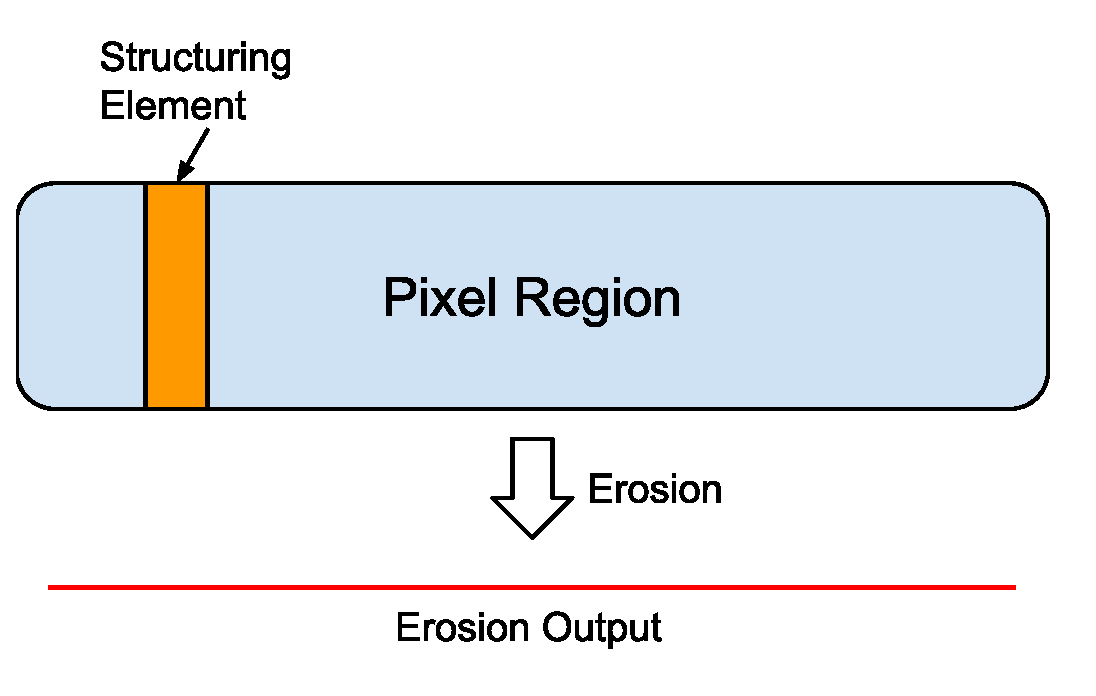
\includegraphics[width=0.8\linewidth]{gfx/erode}
	\caption{Example of morphological erosion with a rectangular structuring element. 
		Outside blue region is assumed identically zero.}
	\label{fig:erode}
\end{figure}
A comparison of the median filter operation versus the erosion operation is illustrated in Figure~\ref{fig:medfilt}.
\begin{figure}\centering
    \includegraphics[width=0.75\columnwidth]{gfx/medfilt}
    \caption{Binary Median Filter versus Morphological Erosion example, showing how at least $N \times N-1$ pixels are required to ``survive'' the operation.}\label{fig:medfilt}
\end{figure}
This step provides much of the denoising one might otherwise apply at substantial computational expense earlier in the process, which is important for rapid processing of terabytes of data whether online or offline.

\subsection{Morphological Dilation}\label{sec:dilate}
While erosion removes thin or isolated features in an image, dilation is a thickening operation that connects small gaps in $A$ according to $B$
\begin{equation}\label{eq:dilate}
A \oplus B = \bigcup_z (B)_z.
\end{equation}
Imagine a peg in the center pixel of the structuring element--the result of dilation is that any place touched by any pixel of the structuring element as the peg is translated within $A$ is declared binary True.
A cartoon example of morphological dilation is shown in Figure~\ref{fig:dilate}. 
\begin{figure}\centering
    \includegraphics[width=0.7\linewidth,trim=10 0 10 0,clip]{gfx/dilate}
    \caption{Dilation example with orange 5 pixel disk SE. 
            Dilation output is green chamfered bar 5 pixels wide due to SE and one-pixel wide input.}\label{fig:dilate}
\end{figure}
Note that even if the red line in Figure~\ref{fig:dilate} had a break up to one-half the diameter of the structuring element, the continuous green form seen at the bottom of Figure~\ref{fig:dilate} would result. 

\subsection{Morphological Opening}
Morphological opening is an idempotent set operation expressed by erosion \eqref{eq:erosion} followed by dilation \eqref{eq:dilate}.
\begin{equation}\label{eq:open}
A \circ B = \left(A \ominus B \right) \oplus B.
\end{equation}
Observe the rounded corners in the green output of the opening example in Figure~\ref{fig:opening}.
\begin{figure}\centering
    \includegraphics[width=0.7\linewidth,trim=70 20 50 50,clip]{gfx/open}
    \caption{Opening example with disk SE. Opening output is green rounded rectangle.}\label{fig:opening}
\end{figure}
The rounded protrusion at the upper left represents the partial fitting of the SE into the notch into the input $A$.
Heuristically, erosion retains pixels where the center of the SE touches when the SE fits within the region $A$.
Opening keeps all the pixels the SE touches when the SE fits within $A$.

\subsection{Morphological Closing}\label{sec:close}
Morphological closing is an idempotent set operation expressed by dilation \eqref{eq:dilate} followed by erosion \eqref{eq:erosion}
\begin{equation}\label{eq:close}
A \bullet B = \left(A \oplus B \right) \ominus B.
\end{equation}
Closing is heuristically represented by passing the SE completely outside and along the exterior-like rolling the disc SE in Figure~\ref{fig:closing} and filling in gaps to meet the SE.
\begin{figure}\centering
\includegraphics[width=0.7\linewidth,trim=50 0 50 0,clip]{gfx/close}
\caption{Closing example with orange disk SE. Closing output is green concave shape.}\label{fig:closing}
\end{figure}
Morphological closing fills in interior oases that may have occurred due to noise or random intensity behavior at the optical flow thresholding step.
This is physically justified by that aurora is not filled with small holes.
The smallest plausible auroral feature size is $\gg$ 1 pixel for the 9 degree field of view chosen for each HiST camera.
The filling operation implemented by closing is important for the next step which qualifies Alfvénic arc plausibility based on the amount of aurora in view that is moving together.

\subsection{Connected Components Criterion}\label{sec:blob}
Alfvénic aurora is likely to occur as a long sinuous continuous thin feature in the field of view.
The Alfvénic arc may split or flame and intensity may be large or small.
We choose as our criteria a region of thin, rapidly moving aurora of more than 100 contiguous pixels.
At this time we do not impose a shape criteria as this may discard some of the wide variety of shapes Alfvénic aurora can take on.
Such a specific morphology classifier would be a future subsequent step.

We declare as connected any region of contiguous 8-connected pixels.
8-connected neighbors mean any pixel touching a face or corner of another pixel as depicted in Figure~\ref{fig:8conn}.
\begin{figure}\centering
	\includegraphics[width=0.8\linewidth,trim=0 0 10 0,clip]{gfx/4conn8conn}
	\caption{Left: 4-connected neighbor pixels. Right: 8-connected neighbor pixels.}\label{fig:8conn}
\end{figure}
Connected component analysis (CCA) computes the size of the oriented minimum bounding box containing the convex hull of an 8-connected pixel region representing the declared foreground (target) pixel \citep{gonzalezwoods}. 
The cartoon in Figure~\ref{fig:connblob} of the convex hull (outlined in purple) of connected pixels is enclosed by the minimum bounding box (outlined in green).
\begin{figure}\centering
	\includegraphics[width=\linewidth,trim= 10 0 10 0,clip]{gfx/connblobcartoon}
	\caption{Example of CCA--upper left pixel group is rejected as having too small convex hull.  Lower right pixel group enclosed in green bounding box is accepted as having sufficiently large convex hull.}\label{fig:connblob}
\end{figure}
Observe how the upper left group of connected pixels has a convex hull yet passes through CCA, since the area of the minimum bounding box is too small. 
In our implementation we require that
\begin{equation}
A < A_{bb} < B
\end{equation}
where $A=100$ and $B=4\times 10^5$ are the minimum and maximum area of the CCA bounding box for each region area $A_{bb}$.
The CCA area minimum threshold keeps isolated clutter regions with a small minimum bounding box from being declared a target.
The CCA area maximum threshold mitigates dataframe-wide shifts in the cross-ambiguity that occur during large shifts in the self-ambiguity.

\subsection{Discriminator Output}\label{sec:discout}
The decision stream from section~\ref{sec:blob} is written to an HDF5 file.
A $64 \times 64$ pixel preview video of frames tagged in the HDF5 file is generated for human consumption via a Google Drive upload.
The bottom block in Figure~\ref{fig:blockcv} corresponds to the input of section~\ref{sec:inv}, where quantitative analysis of the auroral features continues.
\begin{figure}\centering 
    %the \par is necessary after each text to make the \baselineskip take effect
    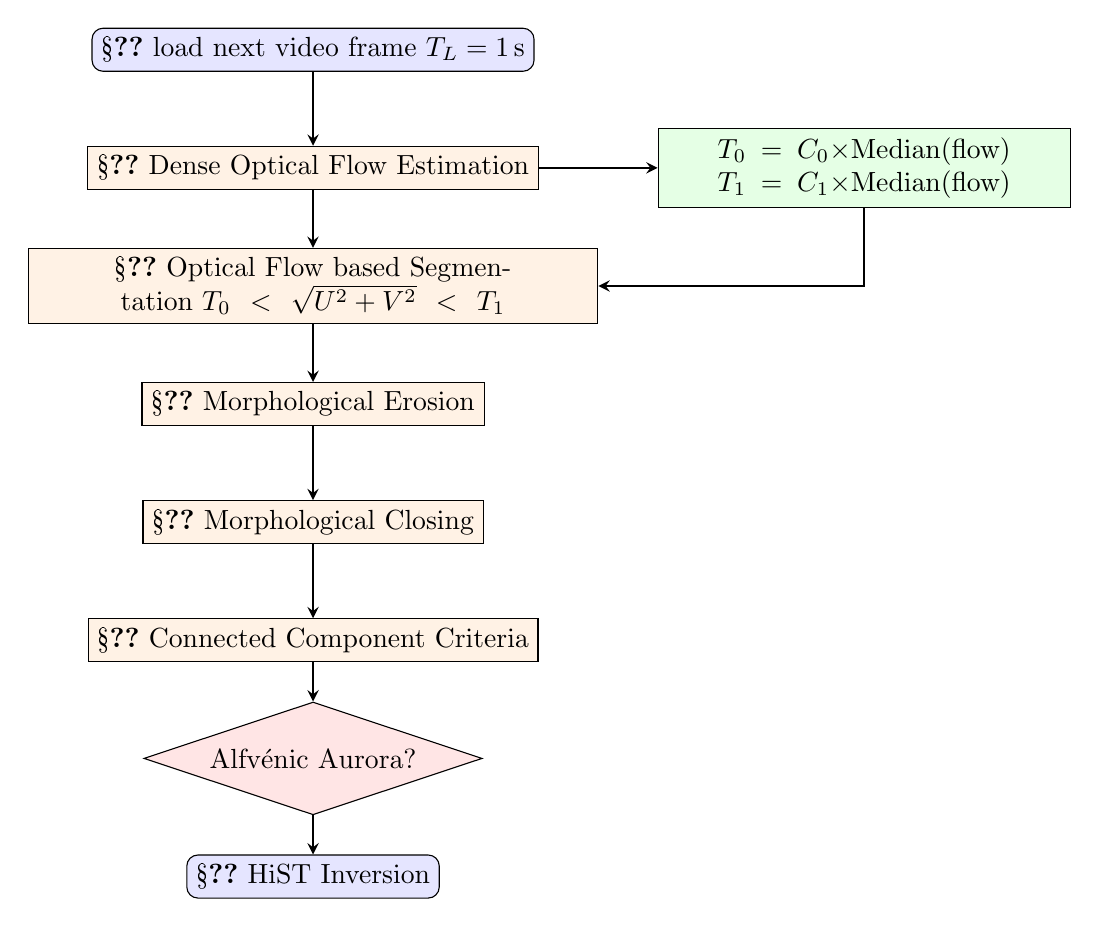
\begin{tikzpicture}[node distance=1.5cm, auto]
    
    \node (in) [startstop] {§\ref{sec:load} load next video frame $T_L=\unit[1]{s}$ \par};
    
    \node (flow) [process, below of=in] {§\ref{sec:of} Dense Optical Flow Estimation \par };
    
    \node (med) [compute, right of=flow, xshift=5.5cm, text width=5cm] { $T_0 = C_0 \times$Median(flow) $T_1 = C_1 \times$Median(flow) \par };
    
    \node (seg) [process, below of=flow,text width=7cm]{§\ref{sec:seg} Optical Flow based Segmentation $ T_0 < \sqrt{U^2 + V^2} < T_1 $ \par};
    
    \node (erode) [process, below of=seg]{§\ref{sec:erode} Morphological Erosion \par};
    
    \node (close) [process, below of=erode]{§\ref{sec:close} Morphological Closing \par};
    
    \node (blob) [process, below of=close]{§\ref{sec:blob} Connected Component Criteria \par};
    
    \node(detect) [decision, below of=blob]{Alfvénic Aurora? \par};
    
    \node(inv) [startstop,below of=detect]{§\ref{sec:hist} HiST Inversion \par};
    
    %
    
    
    \draw[arrow] (in) -- (flow);
    \draw[arrow] (flow) -- (med);
    \draw[arrow] (med) |- (seg);
    \draw[arrow] (flow) -- (seg);
    \draw[arrow] (seg) -- (erode);
    \draw[arrow] (erode) -- (close);
    \draw[arrow] (close) -- (blob);
    \draw[arrow] (blob) -- (detect);
    \draw[arrow] (detect) -- (inv);
    
    \end{tikzpicture}
    
    \caption{Block diagram of  Alfvénic aurora detection algorithm.}
    \label{fig:blockcv}
\end{figure}




\cleardoublepage

\chapter{Feasibility of Reconstructing Fast Fine Scale Auroral Precipitation}
\label{chapter:sim}
\thispagestyle{myheadings}

\graphicspath{{Simulation/}}

\epigraph{I can now demonstrate the great advantage of parallactic pictures. With known star backgrounds, we can estimate not only the auroral heights, but also their locations. We take good picture of intense auroras with an exposure time of only one fifth of a second. Of all cameras I brought with me, the simplest is the best.
It was not at all easy to lay down 4310 meter telephone cables between our two stations during winter and to take them up again.
On every night that auroral displays were in view, I had to find a star, or some star patterns in the middle of the auroras. As soon as that was done, I called Birkeland and asked him to point his camera toward that star. Shortly thereafter I would say: ``Get ready,'' then ``Take the first picture.'' Normally we took several simultaneous pictures from both stations.}{Størmer 1911 translated by \citet{egeland2013}}

We present a feasibility study for a high frame rate, short baseline auroral tomographic imaging system useful for estimating parametric variations in the precipitating electron number flux spectrum of dynamic auroral events. 
Of particular interest are auroral substorms, characterized by spatial variations of order \unit[100]{m} and temporal variations of order \unit[10]{ms}.  
These scales are thought to be produced by dispersive Alfvén waves in the near-Earth magnetosphere. 
The auroral tomography system characterized in this paper reconstructs the auroral volume emission rate to estimate the characteristic energy and location in the direction perpendicular to the geomagnetic field of peak electron precipitation flux using a distributed network of precisely synchronized ground-based cameras. 
As the observing baseline decreases, the tomographic inverse problem becomes highly ill-conditioned; as the sampling rate increases, the signal-to-noise ratio degrades and synchronization requirements become increasingly critical. 
Our approach to these challenges uses a physics-based auroral model to regularize the poorly-observed vertical dimension.  
Specifically, the vertical dimension is expanded in a low-dimensional basis consisting of eigenprofiles computed over the range of expected energies in the precipitating electron flux, while the horizontal dimension retains a standard orthogonal pixel basis.  
Simulation results show typical characteristic energy estimation error less than 30\% for a 3~km baseline achievable within the confines of the Poker Flat Research Range, using GPS-synchronized Electron Multiplying CCD cameras with broad-band BG3 optical filters that pass prompt auroral emissions.

\section{Introduction}

Previous high speed ISR/camera data fusion efforts have used a single high-speed camera \citep{semeter2008,akbari2013,dahlgren2013}.
Auroral tomography with multiple cameras and ISR has previously been accomplished at low speed \citep{bjornthesis,wedlund2013}.
Studies of the aurora using two or more cameras with overlapping fields of view (FOV) were carried out in earnest from 1910 onward \citep{stormer1930}.
More recent work focused on the formal application of tomographic techniques \citep{frey1996,doe1997,bjorn1998,semeter1999,hirsch2016}.
Auroral tomography provides a means of accessing time-dependent information about remote auroral acceleration processes.
In this technique, common volume measurements of the aurora from multiple ground-based imagers are used to reconstruct the wavelength-dependent ionospheric volume emission rate (VER).
VER depends on the energy flux distribution of the precipitating magnetospheric electrons that have undergone a particular acceleration process, gaining high enough energy to penetrate deep into the ionosphere, giving rise to the auroral emissions via collisional and kinetic interactions with neutral species and ions.
The VER reconstruction is used together with a physics-based model of precipitating magnetospheric electrons to estimate the spatial distribution and characteristic energy of the primary electron differential number flux.
Estimation and measurements of the precipitation characteristic energy have been used \citep{chaston2003,mcfadden1999} as a conduit to understand mechanisms driving auroral morphology at the finest spatiotemporal scales.
Figure~\ref{fig:priortomo} represents the relation of prior work in this field to the advances made in this dissertation in Figure~\ref{fig:thistomo}.
The ability of the HiST system to simultaneously obtain estimates of precipitating flux characteristics vs. time \textit{and} space \citep{hirsch2016} are necessary to characterize the evolution of dispersive Alfvén waves in the lower magnetosphere accelerating electrons that cause the microstructure seen in the lower ionospheric aurora \citep{semeter2012}.
\begin{figure}\centering 
    %the \par is necessary after each text to make the \baselineskip take effect
    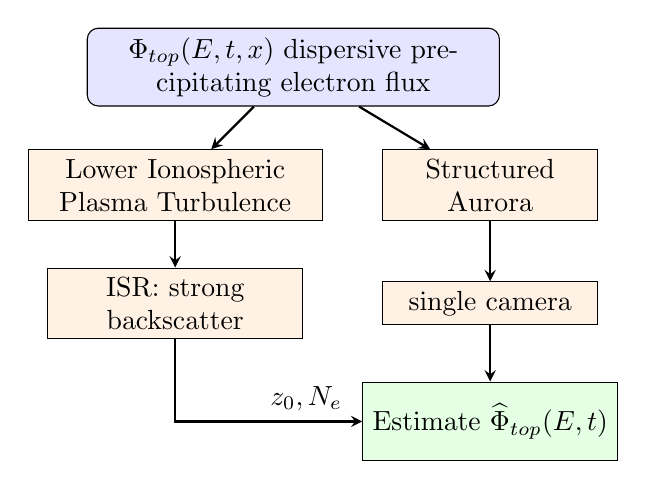
\begin{tikzpicture}[node distance=1.5cm, auto]
    
    \node (phi) [startstop,text width=5cm] {$\Phi_{top}(E,t,x)$ dispersive precipitating electron flux \par};
    
    \node (ver) [process, below of=phi,text width=2.5cm,xshift=2.5cm] { Structured Aurora \par };
    \node (turb)[process, left of=ver, text width=3.5cm,xshift=-2.5cm]{ Lower Ionospheric Plasma Turbulence \par};
    
    \node(isr) [process, below of=turb, text width=3cm] { ISR: strong backscatter \par};
    
    \node (onecam) [process, below of=ver, text width=2.5cm] { single camera \par };

	\node (oneinv) [compute, below of=onecam,text width=3cm] { Estimate $\widehat{\Phi}_{top}(E,t)$ \par};
    
    \draw[arrow] (phi) -- (turb);
    \draw[arrow] (turb)--(isr);
    \draw[arrow] (isr)|-(oneinv) node[pos=0.85, above] {$z_0, N_e$};
    
    \draw[arrow] (phi) -- (ver);
    \draw[arrow] (ver) -- (onecam);
    \draw[arrow] (onecam) -- (oneinv);

    
    \end{tikzpicture}
    
    \caption{Prior work in single camera, single flux tube precipitating electron flux estimation vs. time.}
    \label{fig:priortomo}
\end{figure}

\begin{figure}\centering 
	%the \par is necessary after each text to make the \baselineskip take effect
	\begin{tikzpicture}[node distance=1.5cm, auto]
	
	\node (phi) [startstop,text width=5cm] {$\Phi_{top}(E,t,x)$ dispersive precipitating electron flux \par};
	
	\node (ver) [process, below of=phi,text width=2.5cm,xshift=2.5cm] { Structured Aurora \par };
	\node (turb)[process, left of=ver, text width=3.5cm,xshift=-2.5cm]{ Lower Ionospheric Plasma Turbulence \par};
	
	\node(isr) [process, below of=turb, text width=3cm] { ISR: strong backscatter \par};
	
	\node (cam) [process, below of=ver, text width=2.5cm] { multiple cameras \par };
	
	\node (caminv) [compute, below of=onecam,text width=3cm] { Estimate $\widehat{\Phi}_{top}(E,t,x)$ \par};
	
	\draw[arrow] (phi) -- (turb);
	\draw[arrow] (turb)--(isr);
	\draw[arrow] (isr)|-(caminv) node[pos=0.9, above] {$N_e$};
	
	\draw[arrow] (phi) -- (ver);
	\draw[arrow] (ver) -- (cam);
	\draw[arrow] (cam) -- (caminv);
	
	
	\end{tikzpicture}
	
	\caption{Thesis work in multi-camera precipitating flux estimation vs. time and space.}
	\label{fig:thistomo}
\end{figure}


The reconstruction problem of Figure~\ref{fig:thistomo} is challenging owing to uncertainties in model assumptions and the solution non-uniqueness that arises from the constrained viewing geometry.
The use of a first-principles based physics model was motivated in part by the limited observation in the direction along the geomagnetic field $B_\parallel$.
The short distance between cameras was motivated by the desire to get the highest feasible resolution in the direction perpendicular to the geomagnetic field $B_\perp$ as simulated in Figure~\ref{fig:camres}.
These data inversion techniques provide the first realizable method of obtaining a persistent two-dimensional (energy, $B_\perp$) high resolution morphology estimate of the rapidly evolving electron precipitation above the ionosphere at the smallest ground-observable scales.

Auroral morphologies can be described in a Cartesian coördinate system, with axis $B_\parallel$ oriented along the Earth's local magnetic field $B$.
The HiST phase 1 system was deployed on Poker Flat Research Range (PFRR) with the configuration of Figure~\ref{fig:histloc}.
\begin{figure}
	\includegraphics[width=\linewidth,trim=0 360 0 0,clip]{gfx/3sites}
	\caption{Location of HiST and PFISR at PFRR, Chatanika, AK. PFRR (65.1$^\circ$N, -147.5$^\circ$W) is \unit[30]{km} N-NE of Fairbanks, AK.}\label{fig:histloc}
\end{figure}
At PFRR, the inclination of the E-layer magnetic field is $77.5^\circ$, so the $B_\parallel$ axis is tipped $12.5^\circ$ from the local geographic vertical axis toward magnetic south.
The $B_\perp$ axis is defined to be orthogonal to $B_\parallel$ and coplanar with the cameras.
In auroral literature the ``width'' of auroral features refers to extent in the $B_\perp$ direction, and we follow this convention.

Prior work in auroral tomography \citep{jones1991,semeter1999,frey1998} has focused almost exclusively on mesoscale features of $\unit[10^4]{m}$ width recorded with typical sampling periods of order 1..\unit[30]{s}, with sensor baselines of 50..\unit[150]{km}.
The peak auroral emission intensity typically lies in the altitude range of approximately 100..\unit[300]{km}.
The $B_\parallel$ profile of the arc is dependent on the electron beam differential number flux and the characteristics of the neutrals and ions with which the precipitating particles interact.
An active auroral display embodies a vast hierarchy of spatial scales.
The global auroral oval is of order $\unit[10^5]{m}$ width as measured along magnetic latitude from the poleward to equatorward edges.
Dynamic fine-scale features embedded in an auroral breakup of $\unit[10^2]{m}$ width are typically observed during the substorm expansion phase \citep{semeter2008}.
Anthropogenic aurora of $\unit[10^2]{m}$ width has been observed from HAARP stimulus \citep{pederson2010,kendall2010}.
A complete theory of the aurora must account for variations at all scales inherent in the phenomena.
Although our theoretical understanding of global and mesoscale variability, and its drivers in the solar wind and magnetosphere, is well developed \citep{borovsky1993}, the physics underlying decameter-scale structure embedded within active auroral displays remains incomplete.

Auroral structures of sub-\unit[100]{m} width have been known to exist for decades \citep{maggsdavis1968,trondsendis}, and are seen regularly in long-term observations with modern cameras.
An example of a thin \unit[100]{m} wide auroral structure exhibiting rapid lateral motion is shown in the image sequence of Figure~\ref{fig:perspTrans}.
Note the substantial change in appearance of the arc in $1.5$ seconds, corresponding to a $5^\circ$ change in observer perspective, or about \unit[10]{km} in the $B_\perp$ dimension assuming \unit[120]{km} apparent auroral feature altitude.
%
An example of flaming aurora \citep{omholtbook,dahlgren2013} evolving over \unit[600]{ms} is shown in Figure~\ref{fig:perspFlame}.
%Both of these examples were recorded during the expansion phase of an auroral substorm.
%
% X1387_032307_112015.36_full_30fps.avi
% convert -normalize X1387*.avi[1132] 1132.png
% convert -normalize X1387*.avi[1147] 1147.png
% convert -normalize X1387*.avi[1162] 1162.png
% convert -normalize X1387*.avi[1177] 1177.png
% montage anno_11*.png -trim -tile 4x1 -geometry +1+0  anno_trans.png
\begin{figure*}\centering
    \includegraphics[width=\textwidth]{gfx/2007-03-23breakup}
    \caption{Radical change in perspective for \unit[100]{m} structure in \unit[1.5]{s} due to apparent $B_\perp$ transverse motion \citep{semeter2012,semeter2008}. 
    Contours are centered on local magnetic zenith.}
	\label{fig:perspTrans}
\end{figure*}
%
% generate figure 2.
%
% convert /tmp/CMOSvideo-0223.png -crop 900x550+880+610 flame100615440.png
% convert /tmp/CMOSvideo-0233.png -crop 900x550+880+610 flame100615640.png
% convert /tmp/CMOSvideo-0243.png -crop 900x550+880+610 flame100615840.png
% convert /tmp/CMOSvideo-0253.png -crop 900x550+880+610 flame100616040.png
% python fiducial.py
% montage anno_flame10061*.png -trim -tile 4x1 -geometry +1+0  anno_flame.png
%
%
\begin{figure*}\centering
    \includegraphics[width=\textwidth]{gfx/2011-03-01flame}
    \caption{Flaming aurora evolution over \unit[600]{ms} \citep{dahlgren2013}.
             Contours are centered on local magnetic zenith.}
    \label{fig:perspFlame}
\end{figure*}

Auroral acceleration occurs mainly in the altitude regime from 1000..\unit[40000]{km} \citep{lysak2011}, with DAW acceleration occurring mainly in the 1500..\unit[7000]{km} altitude range \citep{semeter2012}.
While the techniques of this system do not directly measure the acceleration regime, they do measure the outcomes of the acceleration.
The physics model based iterative reconstruction employed allows reconstructing particle flux at \unit[1000]{km} altitude, below which particle acceleration is negligible.
The reconstruction occurs over a sufficiently wide swath of sky (and can be widened by adding more cameras) to help characterize DAW structure in the lower magnetosphere.
%TODO block diagram showing magnetosphere

The tomographic techniques described in this dissertation contribute to understanding how such ephemeral fine-scale structure emerges in the incoming particle flux.
The observational requirements for a tomographic imaging system capable of resolving these scales are extreme, and the resulting inverse problem is highly ill-conditioned.
Section~\ref{sec:hist} presents the High Speed Tomography system (HiST) hardware \citep{hirsch2016}.
Sections~\ref{sec:flame} and~\ref{sec:transverse} comprise a feasibility study for a high frame-rate, short baseline, auroral tomography system.
Through simulation and modeling, we demonstrate that Electron Multiplying CCD (EMCCD) camera technology coupled with a physics-based regularization scheme is capable of resolving electron differential number flux dynamics of order \unit[100]{m} and \unit[10]{ms}.
The highest sensitivity cameras especially suitable for weak filtered auroral emissions are EMCCD-based.
EMCCD cameras are the core of the HiST system, along with GPSDO synchronization and embedded vision algorithms.

\section{Forward Model}\label{sec:fwd}
For the ill-conditioned problem produced by cameras with \unit[3]{km} spacing over \unit[100]{km} from the target of interest, regularization of the poorly observed vertical dimension is a necessary step to get a tractable inversion in terms of computational effort and error bounds.
We fashion a set of eigenprofiles from a problem comprised of linear differential equations by first making the assumption that production $p_{ij}$ and loss $l_{ij}$ for prompt emissions at steady state are related by
\begin{equation}\label{eq:continuity}
p_{ij} - l_{ij} = 0
\end{equation}
for the j\textsuperscript{th} excitation process of the i\textsuperscript{th} species.
The eigenprofiles are used as basis functions \citep{dahlgren2013} in a linear system tying together ground-observed auroral intensity to auroral volume emission rate via a known viewing geometry.
We can solve for the coefficients that correspond to the differential number flux for each log-spaced energy bin, yielding estimated differential number flux $\hat{\Phi}_{top}(B_\perp,E)$ for each new set of camera images.

To model the excitation rates due to primary electron precipitation, we use the 1-D TRANSCAR model \citep{lilensten2002,zett2007,zett2008,dahlgren2013,lummmerzheim1994}. 
Primary considerations for use of TRANSCAR include that 192 spectra are derived \citep{zettdis} from the excitation rates modeled by TRANSCAR. 
The use of a large number of spectra is important to maximizing the information available from a broadband optical filter such as the BG3 that passes numerous prompt line emissions.
The TRANSCAR hybrid kinetic/fluid time-dependent ionosphere model becomes more relevant in future studies incorporating joint observations with instruments such as incoherent scatter radar. 
Because a key requirement of the system is capturing order \unit[10]{ms} auroral dynamics, it was desirable to capture and incorporate the largest number of spectra possible to increase SNR at high frame rates.
TRANSCAR is a physics-based model of six positive ion species and their neutral parents: O\textsuperscript+, H\textsuperscript+, N\textsuperscript+, N$^+_2$, NO\textsuperscript+, O$^+_2$ along with electrons e$^-$ using the charge neutrality \citep{zett2007,blelly1996a,lilensten2002} of plasma $n_e = \sum_S n_s$. 
An 8-moment model \citep{blelly1996a} encompasses thermal diffusion effects so that important heat flows are captured \citep{zett2007}.
The TRANSCAR excitation rates and eigenprofiles used in this feasibility study are computed once for a particular set of geophysical parameters in an offline manner, which takes about 30 minutes using the idle CPU cycles of office PCs arranged in a compute cluster via GNU Parallel \citep{tange2011a}.
The rest of the forward model is implemented in about 2 seconds. 
The data inversion that must be executed for each observation time step must be done on-line for each new observation and takes about one minute on a desktop PC, depending on the number of cells in the projection matrix $\mathbf{L}$.

The close-spaced optical instruments used in this study yield persistent observations of precipitation process outcomes \citep{tanaka2011,wedlund2013} complementing on-orbit and rocket-borne \textit{in situ} measurements with a broader spatiotemporal context, along with improved $B_\perp$ resolution over widely spaced ground-based imagers.
Observation of a typical rapidly moving (several km/s) auroral feature implicitly requires a frame rate on the order of \unit[100]{Hz} for a narrow $9^\circ$ FOV and megapixel-class imager. 
Cameras comprising a multi-camera tomography system must have their frame start/end exposure times known to better than 1/10\textsuperscript{th} of a single frame.
Data inversion with poor time synchronization has limited scientific utility since the emissions observed at time $t_0$ at HiST0 will be smeared together with the results at time $t_0+\epsilon$ at HiST1 due to timing error $\epsilon$.
The camera site spacing is chosen based on the forward model described in this section along with practical facility availability. 

The auroral target of interest is taken to operate within the following first-order constraints:
\begin{enumerate}
    \item Auroral behavior in the $B_\parallel$ dimension is strongly influenced by time-dynamic electron particle penetration \citep{lilensten2002}, as modeled by TRANSCAR. Time of flight difference between high energy and low energy particles in the lower magnetosphere at time scales less than order \unit[10]{ms} have been observed \citep{peticolas2000}. 
    The tomographic process gives information on vertical structure not available in zenith-oriented line integrations alone as in \citet{peticolas2000}, so our technique will capture dynamics with frame rates to at least \unit[100]{Hz}.
    \item Precipitating e\textsuperscript{-} acceleration has taken place above the uppermost altitude cell of the 1-D model, implying that thermospheric and mirroring forces are neglected \citep{lilensten2002,swift1975}
    \item Auroral behavior in the $B_\perp$ dimension is dominated by collisionless processes above the ``top'' of the ionosphere (altitude $>1000$~km) \citep{mozer1998,ergun2002}
\end{enumerate}
With these constraints in mind, we continue with a discussion of the quantitative particulars of the models and algorithms used in this feasibility study. 

%
\begin{figure}\centering 
    %the \par is necessary after each text to make the \baselineskip take effect
    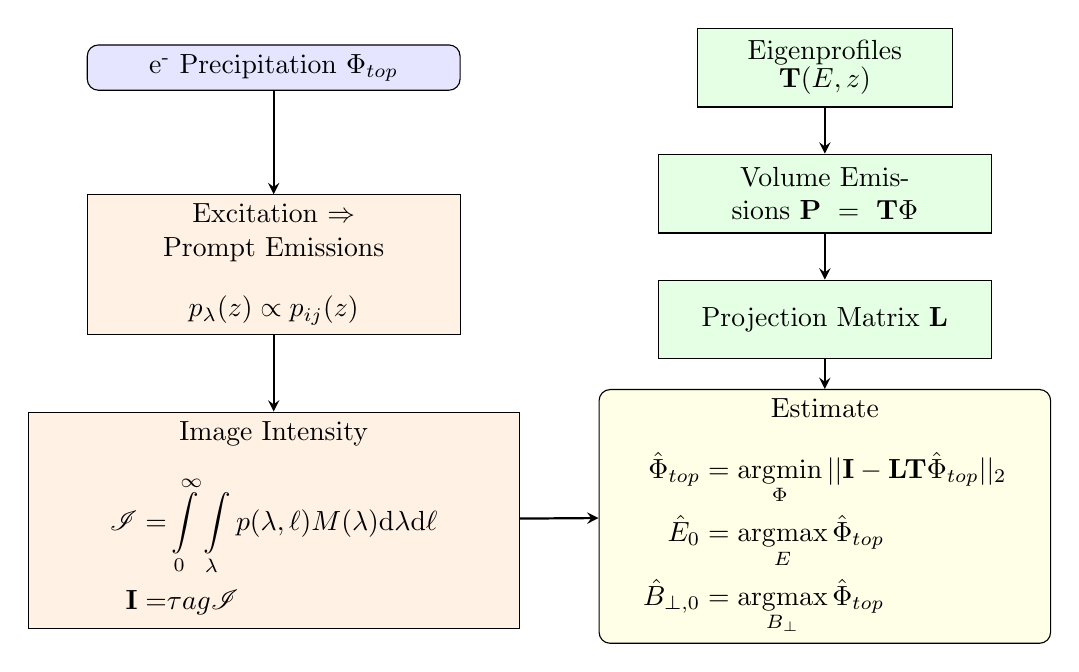
\begin{tikzpicture}[node distance=2cm, auto]
    
    \node (in) [startstop, text width=4.5cm] {\baselineskip=10pt e\textsuperscript{-} Precipitation $\Phi_{top}$ \par};
    \node (p) [process, below of=in, text width = 4.5cm,yshift=-0.5cm] {\baselineskip=12pt Excitation $\Rightarrow$ Prompt Emissions \[ p_\lambda(z) \propto p_{ij}(z) \] \par };
    \node (B) [process, below of=p, text width=6cm, yshift=-1.25cm]{\baselineskip=10pt Image Intensity \begin{align*} 
    	\mathscr{I} =&   \int_0^\infty \int_\lambda p(\lambda,\mathbf{\ell}) M(\lambda) \mathrm{d} \lambda \mathrm{d}\ell \\
    	\mathbf{I} =& \tau a g \mathscr{I}
    	\end{align*}
    	\par};
    %
    \node (eig) [compute, right of=in, text width=3.cm,xshift=5.cm] {\baselineskip=10pt Eigenprofiles $\mathbf{T}(E,z)$ \par};
    \node (P) [compute, below of=eig, text width=4cm,yshift=0.4cm] {Volume Emissions $\mathbf{P} = \mathbf{T}\Phi$};
    \node (L) [compute, below of=P, text width=4cm,yshift=0.4cm] {Projection Matrix $\mathbf{L}$};
    \node (min) [estimate,text width=5.5cm, below of=L,yshift=-0.5cm] {\baselineskip=12pt Estimate  \begin{align*} \hat{\Phi}_{top} &= \argmin_\Phi ||\mathbf{I}-\mathbf{LT}\hat{\Phi}_{top}||_2 \\
        \hat{E}_0 &= \argmax_E \hat{\Phi}_{top} \\
        \hat{B}_{\perp,0} &= \argmax_{B_\perp}  \hat{\Phi}_{top}
        \end{align*} \par};
    
    %
    \draw[arrow] (in) -- (p);
    \draw[arrow] (p) -- (B);
    \draw[arrow] (B) -- (min);
    %
    \draw[arrow] (eig) -- (P);
    \draw[arrow] (P) --(L);
    \draw[arrow] (L) -- (min);
    \end{tikzpicture}
    \caption{Block diagram of HiST auroral tomography forward model and data inversion.}
    \label{fig:overall}
\end{figure}

Referring to the left column of Figure~\ref{fig:overall}, the forward model input $\Phi_{top}$ is generated using a parameterization \citep{strickland1993} with representative values shown in Figure~\ref{fig:fwdstrick}, where the location in energy of peak differential number flux is known as the characteristic energy $E_0$.
%
% python gridaurora/eFluxGen.py ../histfeas/in/demo_flux.h5
\begin{figure}\centering
    \includegraphics[width=\columnwidth,trim=0 0 50 20,clip]{gfx/hirsc6}
    \caption{Input differential number flux for beams with $E_0\in$ \{500, 1000, 2500, 5000, 10000\}~eV \citep{strickland1993}.}\label{fig:fwdstrick}
\end{figure}
%
The physical process generating $p_\lambda(z)$ in the second block of the left column of Figure~\ref{fig:overall} is modeled in TRANSCAR \citep{zett2007,blelly1996a,lilensten2002} and represented by the eigenprofiles $\mathbf{T}$ in the upper right block of Figure~\ref{fig:overall}, with line-integrated modeled spectra for each beam energy shown with and without BG3 filtering in Figure~\ref{fig:spectra}.
%
% python test_calcemissions.py ~/code/histfeas/test/data/ 1613.5 -t 0 -m spectra1d
%
\begin{figure}
    \includegraphics[width=\columnwidth,trim=0 10 0 0,clip]{gfx/hirsc7}
    \caption{Auroral Spectrum integrated along flux tube for $E_0=1.6$~keV, with and without BG3 filter.}\label{fig:spectra}
\end{figure} 
%
Some of the brightest features in the aurora are produced by metastable transitions with radiative lifetimes of order \unit[1..10]{s} \citep{vallancejones1974}. 
In Alfvénic aurora, the electron flux rapidly changes ($< \unit[10]{ms}$ scales) in $B_\perp$ and $E_0$, and the intense metastable emissions glow like an high-persistence oscilloscope phosphor, which in a white light sensor can cover up the much fainter prompt emissions that have several orders of magnitude shorter lifetimes.
Each camera was equipped with a BG3 optical filter with the transmission characteristics of Figure~\ref{fig:optTrans} to greatly attenuate these long lifetime features.
In particular, the deep notch in transmission for the long lifetime metastable emissions lines includes \unit[557.7]{nm} and \unit[630]{nm}.
%
% python gridaurora/test_opticalmod.py -m eps
\begin{figure}\centering
    \includegraphics[width=\columnwidth,trim=5 5 5 5,clip]{gfx/hirsc8}
    \caption{Optical system transmission, including BG3 filter, EMCCD window and LOWTRAN modeled atmospheric absorption.}\label{fig:optTrans}
\end{figure}
%
The volume production rate of process $p_{ij}$ integrated over fixed pitch angle $\mu$ resulting from the TRANSCAR model is 
\begin{equation}\label{eq:prodEq2}
p_{ij}(z) =n_i(z) \int \sigma_{ij}(E)\Phi(z,E)\textrm{d}E 
\end{equation}
where $n_i$ is the MSIS90-initialized density of the i\textsuperscript{th} ground-state neutral species (e.g. N$_2$, O$_2$, O). $\sigma_{ij}$ is the electron impact cross section of the $j$\textsuperscript{th} excitation process for the $i$\textsuperscript{th} species \citep{semeter2012}. 
$\Phi(z,E)$ is the pitch angle integrated flux obtained from the 1-D model TRANSCAR \citep{blelly1996a} for 33 log-spaced energy bins $E$ ranging from \unit[58]{eV} to \unit[17.7]{keV} \citep{dahlgren2013}. 
For prompt emissions, we connect excitation rates to optical volume emission rates using~\eqref{eq:continuity} with \citep{zettdis,vallancejones1974} the Einstein coefficients and Franck-Condon factors,
\begin{equation}\label{eq:prompt4}
p_\lambda(z) \propto p_{ij}(z)
\end{equation}

For the lower left block of Figure~\ref{fig:overall}, the photon flux at the $k$\textsuperscript{th} camera pixel is described by a line integral mapped via the lens to angle $\theta_k$, treating the auroral region as optically thin at the wavelengths observable through the optical filtering and LOWTRAN \citep{lowtran7} modeled atmospheric absorption of Figure~\ref{fig:optTrans}.
Considering~\eqref{eq:prompt4} and total transmission $M(\lambda)$ shown in Figure~\ref{fig:optTrans}, the photon flux available at the imaging chip $\mathscr{I}(\theta)$ is
\begin{equation}\label{eq:grayb}
\mathscr{I}(\theta) =  \int_0^\infty \int_\lambda p(\lambda,\mathbf{\ell}) M(\lambda) \textrm{d} \lambda \textrm{d}\ell
\end{equation}
The camera exposure time $\tau$, amplifier gain $g$ and pixel area $a$ are modeled with the output in data numbers $\mathbf{I}$ as:
\begin{equation}\label{eq:dn}
\mathbf{I} = \tau a g \mathscr{I}
\end{equation}
where typical values include $a=(16~\mu\textrm{ m})^2, \tau = 2\times10^{-2}~\textrm{s}, g=1~I / \textrm{e}^- $.

Referring to the right column of Figure~\ref{fig:overall} we assemble projection matrix $\mathbf{L}$ by mapping viewing angle $\theta$ to our discrete EMCCD imaging arrays, and compute the intersection length of each ray \citep{semdis} with the relevant cell of $\mathbf{L}$ using the Cohen-Sutherland line clipping algorithm \citep{cohensutherland,cvutils}.
The dimensions of $\mathbf{L}$ are $N_{cam} N_{cut} \times N_{B_\perp} N_{B_\parallel}$,  where $N_{cam}$ is the number of cameras in the system, $N_{cut}$ is the number of 1-D pixels used from each camera and $N_{B_\perp},N_{B_\parallel}$ are the number of $B_\perp, B_\parallel$ pixels in the grid for the volume emission rate matrix $\mathbf{P}$ .
The IGRF 11 model is incorporated into $\mathbf{L}$ for the Poker Flat Research Range, where the inclination $77.5^\circ$ and declination $19.9^\circ$ of the local geomagnetic field determine the angular coördinates of magnetic zenith. 

The grid of Figure~\ref{fig:Lcam} extends from approximately 90-1000~km altitude, showing the locations used in estimating volume emission rate $\mathbf{P}$ due to the incident differential number flux $\Phi_{top}$.
\begin{figure}
\includegraphics[width=\columnwidth,trim=5 6 5 5,clip]{gfx/Lcam}
\caption{Viewing geometry for the two-camera system at the Poker Flat Research Range, showing selected lines of sight over a decimated reconstruction grid.}\label{fig:Lcam}
\end{figure}
Overlaid on this grid are the decimated 1-D rays corresponding to intensity vector $\mathbf{I(\theta)}$.
For Figure~\ref{fig:Lcam} and the analysis of Section~\ref{sec:transverse} and~\ref{sec:flame}, $N_{cam}=2, N_{cut}=512, N_{B_\perp}=219, N_{B_\parallel}=123$.
This forward model yields ground-observed optical intensity vs. angle due to electron differential number flux $\Phi_{top}(B_\perp,E)$. 
The analysis in Section~\ref{sec:inv} uses observations from ground-based cameras to estimate the unobservable differential number flux $\hat{\Phi}_{top}$ via a minimization algorithm. 

\section{HiST Data Inversion}\label{sec:inv}

To estimate the characteristics of the time-dependent differential electron number flux $\Phi_{top}$ high in the ionosphere where collisionless processes dominate we employ a physics-based regularization scheme. 
The poorly observed $B_\parallel$ dimension is regularized with a linear basis expansion of volume emission rate eigenprofiles calculated by the TRANSCAR model.
The 33 log-spaced energy bins from \unit[58]{eV} to \unit[17.7]{keV} each have a coefficient estimated by our inversion algorithm for each $B_\perp$ location, comprising $\hat{\Phi}_{top}(B_\perp,E)$.
For the simulations of chapter~\ref{chapter:sim}, $\hat{\Phi}_{top}$ has dimensions $(219,33)$.
Regularization along $B_\parallel$ is key to finding a physically plausible solution from the infinitely many possible solutions due to the large null space of the inverse problem.
The data inversion process is outlined in the right column of Fig.~\ref{fig:overall}.
As observed in the middle row of Fig.~\ref{fig:est1dflame}, the volume emission rate is a smooth function of differential number flux and altitude.
The smoothness justifies describing the relationship between the unobservable \textit{in situ} physics and the observable auroral intensity by the Fredholm Integral of the First Kind,
%
\begin{equation}\label{eq:fiefk}
g(s) = \int_a^b K(s,t)f(t)\textrm{d}t
\end{equation}
%
where $f(t)$ is the unknown quantity, $g(s)$ is the observed quantity, and $K(s,t)$ is the kernel through which $g(s)$ is observed, encompassing optical filters, line integration of volume emission rate, and noise. 
For the present auroral tomography problem, we incorporate TRANSCAR eigenprofiles
\begin{equation}\label{eq:eigentranscar}
T(E,z) = \int_{\lambda} p_\lambda(E,z) M(\lambda) \textrm{d}\lambda
\end{equation}
in a representation of total auroral volume emission rate as
%
\begin{equation}\label{eq:fiefkE}
P(z) = \int_0^\infty T(E,z) \Phi_{top}(E)\textrm{d}E
\end{equation}
%
which has the same form as~\eqref{eq:fiefk} and may be discretized in matrix form,
%
\begin{equation}\label{eq:fiefkEmat}
\mathbf{P} = \mathbf{T}\Phi_{top}
\end{equation}
%
The discretized forms are convenient for computer implementation since the continuous integration~\eqref{eq:fiefkE} is represented by matrix multiplication~\eqref{eq:fiefkEmat}.
The BG3 filtered and atmosphere attenuated continuüm of wavelengths is observed at the camera as grayscale intensity
%
\begin{equation}\label{eq:master}
\textbf{L}\textbf{T}\Phi_{top}=\textbf{I}
\end{equation}
resulting in the data numbers $\mathbf{I}$ of~\eqref{eq:dn}.

In general $\mathbf{L}$ and $\mathbf{T}$ are not square, so the inverse $\mathbf{L}^{-1}$ and $\mathbf{T}^{-1}$ are not defined in this underdetermined system.
The ill-conditioned and Hadamard ill-posed nature of the problem arises both from the extreme problem geometry and that there is not a unique tomographic solution for the incident number flux causing an auroral display.
A method for solving such problems via brute force is the use of minimization algorithms \citep{semeter1997}. 
The algorithm selected for this effort is the Limited Memory Broyden-Fletcher-Goldfarb-Shanno algorithm \citep{Byrd1995,Zhu1997,Morales2011}, known as L-BFGS-B \citep{scipy}.
This algorithm was selected based on fast convergence for the large number $(>7000)$ of $\hat{\Phi}_{top}(B_\perp,E)$  parameters to minimize based on an empirical comparison with other contemporary minimization techniques.

For a particular realization of geophysical conditions and choice of differential number flux energy bins $\mathbf{T}$ is obtained from an off-line computation. 
As implicit in \eqref{eq:fiefk}, $\mathbf{T}$ is identical in the forward model and data inversion.
The 1-D slices of the synchronized images from each camera are stacked in column-major vector $\mathbf{I}$. 
The 2-D array $\hat{\Phi}_{top}(B_\perp,E)$ has rows arranged by precipitation energy in eV and columns arranged by $B_\perp$ location in kilometers.
We use L-BFGS-B minimization function
\begin{equation}\label{eq:bmin}
\hat{\Phi}_{top}(B_\perp,E) = \argmin_\Phi||\mathbf{I}-\mathbf{LT}\hat{\Phi}_{top} ||_2 =  \argmin_\Phi ||\mathbf{I}-\hat{\mathbf{I}}||_2
\end{equation}
with the bounds $\Phi \in \left[0,\infty\right)$ is given an initial guess $\Phi_{top}(B_\perp,E) \equiv 0$, and is allowed to run for 10--20 cycles. 
Automated measurements of $E_0$ and $B_{\perp,0}$ are accomplished via a 2-D Gaussian fitter algorithm originally based on MINPACK \citep{Minpack}. 
The region of the maximum differential number flux is fitted with a 2-D Gaussian using a Levenberg-Marquardt least squares algorithm to find the parameters best fitting the peak vicinity of $\hat{\Phi}_{top}$. 
In general, the forward model will have limitations in absolute accuracy with regard to the physical world due to the model assumptions and simplifications necessary to get a tractable computation within time and memory constraints.
We now examine simulations of two types of highly dynamic auroral events to show the feasibility of the HiST system for estimating $E_0$ and $B_{\perp,0}$.

%\section{ISR Data Inversion}\label{sec:isrinv}
Recent work on inversion of auroral observations to estimate the incident precipitation energy flux distribution at the top of the ionosphere includes \citet{zett2007,semeter2012,dahlgren2013,wedlund2013,hirsch2016}. 
An overview of the inversion process needed is
\begin{equation}\label{eq:fiefk1}
\vec{q} = \mathbf{A}\vec{\phi}
\end{equation}
where $\vec{q}$ is a $z \times 1$ column vector of ionization rates--ionization caused by electron precipitation into the ionosphere, and
\begin{equation}\label{eq:fiefk2}
\vec{P} = \mathbf{B} \vec{\phi}
\end{equation}
where $\vec{P}$ is a $z \times 1$ column vector of VER caused by kinetic interactions of precipitating electrons with the ionosphere \citep{wedlund2013}.

The electron precipitation is represented by $\vect{\phi}$, an $E \times 1$ column vector of ionization rates. 
$z$ is the number of altitude bins chosen in the discrete problem. 
$E$ is the number of differential energy bins chosen in the discrete problem. 
$\mathbf{A}$ and $\mathbf{B}$ are each of dimensions $z \times E$.





\citet{partamies2004} omits secondary electrons, since they have energies of less than 100 eV. % [p. 1968 last paragraph]
A significant portion of energy observed by the \unit[32]{eV}..\unit[30]{keV} DMSP particle detector is above \unit[8]{keV} \citep{partamies2004}. % [p.1969 first para].
p. 1964 $$ 1\textrm{mW/m}^2 = 6.24\times10^{12} \textrm{keV/m}^2\textrm{s} $$

\citet{partamies2004} used SPECTRUM, a non-standard FORTRAN 77 program translated by Annika Olsson to Matlab to calculate energy fluxes from the $N_e$ measured by ISR.
\url{http://www.lunduniversity.lu.se/lucat/user/54539ff9da4c67bb5baee00c09f22816}
\url{ftp://ftp.irf.se/pub/perm/ESRAD/SPECTRUM/}



% python figure_flame2.py --load -m fwd optim eps 

\section{Model and Inversion of Flaming Aurora}\label{sec:flame}
We model two time steps of a flaming auroral event with $E_0\in\lbrace{4.5,1.6\rbrace}$~keV. 
The input differential number flux $\Phi_{top}$ is shown in Fig.~\ref{fig:estflame}(a)(c). 
Fig.~\ref{fig:estflame}(b)(d) show the estimated differential number flux $\hat{\Phi}_{top}$ using the L-BFGS-B algorithm. 
%
\begin{figure}\centering
\includegraphics[trim=30 120 100 20,clip,height=0.85\textheight]{gfx/flamesim}
\caption{Flaming aurora simulation with characteristic energy $E_0\in\{4.5,1.6\}$~keV and $B_{\perp,0}=1.0$~km. 
(a)(c): differential number flux $\Phi_{top}$. (b)(d): estimated differential number flux $\hat{\Phi}_{top}$. 
(e)(g): forward modeled VER $\mathbf{P}$.  (f)(h): estimated VER $\mathbf{\hat{P}}$.} \label{fig:estflame}
\end{figure}
%
1-D cuts of $\Phi_{top}$ and $\hat{\Phi}_{top}$ at $B_{\perp}=1.0$~km are shown in Fig.~\ref{fig:est1dflame}(a)(b) respectively to aid in visualizing the characteristic energy $E_0$.
Table~\ref{tab:Jestflame} describes the $E_0$ estimation error.
%
\begin{sidewaystable}\centering
\caption{Simulated estimation error for flaming and translating auroral arcs.} \label{tab:Jestflame}
	\begin{tabular}{llllll}
		\toprule
		$B_{\perp,0}$ [km] & $E_0$ [keV] & $\hat{B}_{\perp,0}$ [km] & $\hat{E}_0$ [keV] & Error $|B_{\perp,0}-\hat{B}_\perp,0|$ [\%] & Error $|E_0-\hat{E}_0|$ [\%] \\
		\midrule
		1.0 & 4.5 & 1.0 & 4.1 & \textless 5 & \textless 10 \\
		1.0 & 1.6 & 1.0 & 1.7 & \textless 5 & \textless 10 \\
		1.55 & 5.0 & 1.55 & 4.67 & \textless 5 & \textless 10 \\
		2.5 & 4.5 & 2.5 & 4.1  & \textless 5 &  \textless 20  \\ 
		2.5 & 1.6 & 2.55 & 1.2 & \textless 5 &  \textless 25  \\ 
		3.75 & 5.0 & 3.7 & 5.7 & \textless 5 & \textless 25 \\
		4.2 & 4.5 & 4.15 & 5.6  & \textless 5 &  \textless 25  \\
		4.2 & 1.6 & 4.1 & 1.15  & \textless 5 &  \textless 30  \\
		\bottomrule
	\end{tabular}
	
\end{sidewaystable}

The estimated volume emission rate $\hat{\mathbf{P}}$ as shown in Figure~\ref{fig:estflame}(f)(h) and as 1-D cuts in Figure~\ref{fig:est1dflame}(c)(d) have morphologically similar characteristics to the forward modeled volume emission rate $\mathbf{P}$ in Figure~\ref{fig:est1dflame}(e)(g), as expected.
We observe that the estimated ground-observed intensity $\hat{\mathbf{I}}$ in Figure~\ref{fig:est1dflame}(e)(f) is within a small factor of the forward model intensity $\mathbf{I}$. 
As summarized in Table~\ref{tab:Jestflame}, $\hat{\Phi}_{top,0}$ has been estimated with $E_0$ error typically less than 30\% for simulated auroral arcs within $2.5^\circ$ of magnetic zenith.

The addition of a third camera at $B_\perp=\unit[10]{km}$ initially does not appear to make a dramatic improvement in increasing the angular range from magnetic zenith for estimating $\hat{\Phi}_{top,0}$. 
It is desirable to extend the estimate of precipitation characteristics to 3-D, which intrinsically motivates incorporating more than 2 cameras into HiST.
As observed in Table~\ref{tab:Jestflame}, the $\hat{\Phi}_{top,0}$ estimate is usable to at least $2.5^\circ$ from magnetic zenith.
It is apparent that a key limit of the $B_\perp$ range of the inversion is keeping the auroral target within the common FOV of the cameras, as is trivially expected. 


\begin{figure}\centering
\includegraphics[trim=50 150 50 40,clip,height=0.875\textheight]{gfx/flamesim1d}
\caption{Flaming aurora simulation, 1-D cuts. 
(a)(b): Estimated differential number flux $\hat{\Phi}$.
(c)(d): Volume emission rate $\hat{\mathbf{P}}$. 
(e)(f): Ground-observed intensity $\mathbf{I}$ for characteristic energy $E_0\in\{4.5,1.6\}$~keV.}\label{fig:est1dflame}
\end{figure}

% python figure_trans2.py --load -m fwd optim eps
\subsection{Model and Inversion of Laterally Translating Aurora}\label{sec:transverse}
The laterally translating aurora simulation was configured with $E_0\equiv \unit[5]{keV}$  and $B_{\perp,0}\in$\{1.55, 3.75\}~km. 
%
\begin{figure}
\centering
\includegraphics[trim=50 140 80 30,clip,height=0.875\textheight]{gfx/transversesim}
\caption{$B_\perp$ translating aurora simulation with characteristic energy $E_0 \equiv \unit[5]{keV}$ and $B_{\perp,0}\in$ \{1.55, 3.75\}~km. 
(a,c): differential number flux $\Phi_{top}$. (b,d): estimated differential number flux $\hat{\Phi}_{top}$. 
(e,g): forward modeled VER $\mathbf{P}$.  (f,h): estimated VER $\mathbf{\hat{P}}$.}%
\label{fig:JPB}
\end{figure}
%
Fig.~\ref{fig:JPB}(a)(c) show the input differential number flux $\Phi_{top}$, resulting in the volume emission rate $\mathbf{P}$ displayed in Fig.~\ref{fig:JPB}(e)(g). 
Fig.~\ref{fig:JPB}(b)(d) shows the estimated differential number flux $\hat{\Phi}_{top}$ using the L-BFGS-B algorithm and two cameras at $B_\perp \in\{0,3\}$ ~km.
Table~\ref{tab:Jestflame} describes the estimated differential number flux results.
The artifacts in $\hat{\Phi}_{top}$ and $\mathbf{\widehat{P}}$ come from the noise deliberately injected into the simulated $\mathbf{I}$. 
These artifacts are smaller in amplitude than the peak closest to the true answer, allowing for $\hat{\Phi}_{top,0}$ to be extracted despite the artifacts.
The estimated volume emission rate $\hat{\mathbf{P}}$ shown in Fig.~\ref{fig:JPB}(f)(h) has morphologically similar characteristics to the forward modeled volume emission rate in Fig.~\ref{fig:JPB}(e)(g), as expected. 


\section{Conclusions}\label{sec:concl}
This chapter shows results from a regularization scheme using the physics encapsulated in TRANSCAR modeled eigenprofiles in a two camera simulation, with testing extended to three cameras for future 3-D work.
We observed estimates of the peak differential number flux $\hat{\Phi}_{top,0}(B_{\perp,0},E_0)$ for an auroral arc in the common FOV of the cameras, with typical error less than 30\% for auroral arcs within $2.5^\circ$ from camera boresight on magnetic zenith. 
TRANSCAR is used in a linear basis expansion of log-spaced energy bins across an energy range observed in the most common auroral events, enabling future extension to incorporate incoherent scatter radar and other instruments to form a meta-instrument for observing the ionospheric short term and long term trends.
This basis expansion is used to regularize the poorly observed vertical dimension, simultaneously enabling  high spatial resolution in $B_\perp$, which is important for capturing the detail in dynamic dispersive auroral events with \unit[10]{ms} temporal scales.
The performance estimates of this feasibility study show that a two camera system at the Poker Flat Research Range with \unit[3]{km} camera separation can give new science insights on multiple fronts, including the highly dynamic electron beam structures driving into the ionosphere.
Specifically, we can estimate the characteristic energy and $B_\perp$ peak location of the differential number flux $\Phi_{top}$.
The new observation techniques include use of filtered broadband optical emissions to select only prompt emissions with fast, highly sensitive EMCCD cameras, enabling the use of high frame rates with cadence of order \unit[10]{ms}.
The modeled HiST instrument is shown to be capable of high resolution electron precipitation characteristic energy estimates along $B_\perp$ within suitable error bounds, while retaining the qualitative morphology of the differential number flux in the spatial and energy domains.
Future work includes extending this estimate to 3-D by utilizing 3-D phantoms in the forward model and 3-D inversion of the 2-D pixel intensity images from the cameras, along with a 3 camera phase II HiST deployment to Poker Flat Research Range for a multi-year autonomous deployment beginning in the 2017 auroral season.

\cleardoublepage

\chapter{Joint ISR-Optical Tomography Analysis}
\label{chapter:fusion}
\thispagestyle{myheadings}

\graphicspath{{Fusion/}}

\epigraph{In order to solve the problem of the cause of the aurora and magnetic perturbations, it was necessary to have at our command simultaneous magnetograms and observations from several suitable polar stations at distances of about 1000 kilometers from one another, and also corresponding material from as many other stations all over the world as it was possible to obtain. I demonstrated namely, that certain well-defined magnetic perturbations that occurred over large portions of the earth might be naturally explained as the effect of electric currents.}{\citep{birkeland1908}}

Alfvén waves are an important mechanism for communicating magnetospheric stress into Earth's upper atmosphere.
A significant fraction of the Alfvénic flux is realized as ionospheric Langmuir turbulence and thin dynamic auroral arcs.
Key signatures of Alfvénic dispersion are revealed in the spatiotemporal structure of the aurora. 
Alfvénic auroral structures are strikingly distinct from auroral arcs produced by quasi-static parallel electric fields.
Distinguishing quasi-static arcs from Alfvénic arcs requires high-speed, high-resolution filtered optical systems to capture prompt emissions.
Coordinated optical and incoherent scatter radar measurements routinely show strong echoes from ionospheric destabilization spatiotemporally associated with Alfvénic aurora.
Such observations suggest a connection between Alfvénic particle flux and destabilization of ion-acoustic and Langmuir (electron-acoustic) waves in the lower ionosphere.
The utility of a ground-based high-speed optical tomography system providing estimates of electron precipitation energy spectral characteristics during Alfvén-wave driven destabilization is demonstrated.

\graphicspath{{Fusion/}}

\section{Introduction}\label{sec:intro}
Thin beams of intense electron precipitation are associated with spatially discrete aurora and families of wave modes arising from the beam-destabilized plasma \citep{akbari2015}.
Incoherent scatter radar (ISR) routinely shows F-region enhancements in the ion-acoustic and plasma line spectra associated with wave mode destabilization due to this intense precipitation \citep{schlatter2014}.
Optical measurements of finely structured prompt auroral emissions are strongly correlated with incoherent scatter radar (ISR) backscatter power \citep{sullivan2008,michell2009,michell2014}.
Fast-sampling auroral tomography systems can estimate particle precipitation differential number flux as a function of space, energy and time based on prompt auroral emissions \citep{hirsch2016}.
It is often difficult to determine the direct mechanism by which the energy of the precipitating particles is transformed into free energy for plasma waves.
The exact mechanism underlying the intensification of ion-acoustic waves regularly observed by ISRs in the form of strong backscattered echoes called NEIALs (Naturally Enhanced Ion Acoustic Lines) is not well understood \citep{michell2014}.
In the case of NEIALs there exist competing theories that relate the free energy to fluxes of soft electron precipitation \citep{akbari2014} or to populations of thermal electrons and ions streaming relative to one another \citep{akbari2012}.

Guided by prior observational and theoretical knowledge of spatiotemporal bounds on ground-observable physics, researchers over the past century \citep{stormer1930,stormer1932} and especially the past decade \citep{lynch2012,donovan2006,dahlgren2008} have infused technological progress into systems designed for better understanding of magnetospheric particle precipitation via optical measurements of aurora.
\citet{semeter2008} used a single \unit[30]{fps} $512 \times 512$ pixel BG3-filtered EMCCD camera with PFISR to study dispersive Alfvén wave (DAW) aurora during an substorm breakup, where thin filaments periodically and rapidly split from the arc. 
The splitting arc optical signature is a manifestation of the dispersion relation of DAW with a spatially periodic structure \citep{semeter2008}.
\citet{dahlgren2013} used bursts of a single \unit[30]{fps} sCMOS $2560 \times 2160$ pixel BG3-filtered camera with Poker Flat ISR (PFISR) to characterize flaming aurora with sub-second time scales.
Flaming aurora \citep{omholtbook,dahlgren2013} is generated by DAW auroral flux with faster high energy particles arriving first in the lower ionosphere.
The MOOSE instrument \citep{michell2014} consists of four co-aimed $190 \times 190$ pixel EMCCD cameras running at 40 frames/s with filters for $\lambda \in \{427.8, 844.6, 630.0\}$~nm and a BG3 filter.
The High Speed Auroral Tomography system (HiST) \citep{hirsch2016} yields estimates of primary precipitating electron differential number flux at \unit[20]{ms} cadence.
Faster frame rates are constrained by the SNR achievable from -60$^\circ$C cooled EMCCD cameras sensitive to single photoelectrons, considering the optical filtering needed to select prompt emissions.

Characterizing various types of tightly $B_\perp$-spaced DAW auroral arcs requires networks of cameras spaced in the \unit[1..10]{km} range as simulated in Figure~\ref{fig:camres}.
The HiST synchronized cameras enable detection of conditions favorable for plasma turbulence from auroral arcs.
Examples of discrete auroral arcs are drawn in Figure~\ref{fig:cartoonmorph}.
\begin{figure}\centering
	\begin{minipage}{0.3\textwidth}\centering
		\includegraphics[width=0.9\columnwidth,trim=150 100 150 100,clip]{gfx/aurora_kinked}
	\end{minipage}
	\begin{minipage}{0.3\textwidth}\centering
		\includegraphics[width=0.9\columnwidth,trim=150 100 150 100,clip]{gfx/aurora_split}
	\end{minipage}
	\begin{minipage}{0.3\textwidth}\centering
		\includegraphics[width=0.9\columnwidth,trim=150 100 150 100,clip]{gfx/aurora_ray}
	\end{minipage}
	\caption{Auroral arc morphologies corresponding to: 
		(a) inverted-V 
		(b) strong Langmuir turbulence 
		(c) streaming upflow}
	\label{fig:cartoonmorph}
\end{figure}
This article presents the first joint analysis of such high-speed, closely spaced multi-camera auroral video using physics model-based iterative reconstruction.
The system is shown to be capable of distinguishing monoenergetic inverted-V electron precipitations (with characteristic energy of several keV) from broadband (tens of eV to several keV) electron precipitations from DAW.
New radar sampling techniques \citep{swoboda2015} enable increasingly fine spatio-temporal resolution suitable for quantifying NEIAL characteristics \citep{schlatter2015}.
ISR measurement cadence of \unit[12]{ms} for ion-line \citep{michell2010} and \unit[200]{ms} for plasma-line \citep{vierinen2016} have been achieved, a factor of 80 improvement over prior plasma-line measurements \citep{nicolls2006}.
Joint optical and ISR measurements targeting NEIALs need to sample faster than \unit[40]{Hz} to capture the temporal dynamics of NEIALs.
Persistent staring automated instruments are required for a practical systems since an entire NEIAL event may last less than half a second \citep{dahlgren2013}.

Joint ISR and high speed filtered optical observations give supporting evidence for apparent connections between DAW aurora and naturally enhanced ion-acoustic lines (NEIALs).
NEIALs are bursty aspect-angle dependent strong ion-line echoes in the lower ionosphere.
Strong echoes in the plasma-line channel accompanied by NEIALs are from Langmuir waves, associated with large fluxes of precipitating electrons \citep{akbari2012}.
The primary electron differential number flux associated with NEIALs has similar sub-second temporal scales and $B_\perp$ scale of \unit[100]{m}.
$B_\perp$ scale width due to anthropogenic heating such as HAARP leads to \unit[100]{m} $B_\perp$ auroral emissions \citep{kelley1995,kendall2010}.
During NEIALs, the ISR fitter algorithms relying upon a Maxwellian ion distribution break down due to non-Maxwellian ion spectrum \citep{knudsen1993}, leading to derived plasma parameters in large error or NaN values.
The mechanisms driving NEIALs are distinct from the electron convection responsible for strong backscatter from Farley-Buneman instabilities arising in the E-region ionosphere below \unit[130]{km} \citep{oppenheim1996,hysell2013}.
Simulation efforts to characterize NEIALs are underway \citep{diaz2008}, but push modern supercomputers such as STAMPEDE to the limits.

\citet{akbari2012} noted open questions on the specific energy transport and deposition processes generating the ionospheric plasma destabilization.
Two possibilities for the energy deposition generating the turbulence are:
\begin{enumerate}
    \item plasma waves intensified directly by primary electron precipitation kinetic processes
    \item plasma waves intensified by secondary suprathermal (hundreds of eV) electrons as a result of the electron beam.
\end{enumerate}
Particle acceleration yielding narrow $B_\perp$ energy flux structure from the magnetosphere into the ionosphere may come from quasi-static electric fields or Alfvén waves.
\citet{akbari2014} speculated that diverse electron precipitation mechanisms may be responsible for driving NEIALs, due to the strong aspect angle dependence of ISR returns.
Rocket observations \citep{knudsen1990} have provided \textit{in situ} measurements distinguishing Alfvén wave accelerated particles from quasi-static accelerated particles.
Since NEIALs may occur for only a few seconds during a substorm, confirmation via \textit{in situ} measurement would take numerous million-dollar rocket launches, each yielding a few minutes of data.
Practical observational means associating Alfvén waves with the turbulence arises from ground-based high speed synchronized cameras used together with ISR.
\graphicspath{{Fusion/}}
%\citet{akbari2012} discussed Langmuir turbulence using low-level radar data using a single high-speed EMCCD camera.
%\citet{dahlgren2013} gave relative estimates of flaming auroral behavior with an EMCCD camera and PFISR-based starting assumptions.
Fast EMCCD camera observations with ISR routinely show thin, highly dynamic aurora with temporal signatures characteristic of DAW aurora.
Shear plasma flows such as occur during reconnection launch Alfvén waves of wavenumber short enough to be seen in $\sim$ 10 degree field of view (FOV) cameras focused on a region about magnetic zenith.
During active solar times, substorms occur frequently enough that multiple Alfvénic aurora may be observed in a single night.
The following subsections describe the instruments and methods used to distinguish inverted-V aurora from the Alfvénic aurora associated with NEIALs.

\FloatBarrier
\subsection{Poker Flat ISR (PFISR)}\label{sec:fuspfisr}
PFISR produces several low-level data products including the complex analog-to-digital converter voltage samples.
At the time, access to the large files containing low-level PFISR data is by request, with radar data accumulating at $\sim \unit[1.5]{MB/s}$ during a typical experiment.
% data: Apr 14 2013  (468530486 + 224263860 + 224263860 + 187839490) bytes / 729 seconds = 1.516 MByte/sec
Madrigal PFISR high-level data products have integration times $\sim \unit[2]{min}$ versus \unit[10..100]{ms} cadence of the low-level PFISR data.
Long integration time is necessary for plasma parameter estimation since incoherent returns from the ionospheric volume target provide return signals far too weak to characterize from a single pulse.
An autocorrelation function (ACF) is built up from the incoherent electron and ion scatterers over tens of seconds.
Taking the Fourier transform of the ACF the power spectral density (PSD) is obtained, with a notional PSD from a quiet ionosphere shown in Figure~\ref{fig:isrmorph}(a).
An ACF fitting algorithm provides estimates of electron number density, electron and ion temperature and ion velocity.

These plasma parameter estimates break down when turbulent plasma leads to a breakdown in the parameter fitter, which expects PSDs having morphology similar to Figure~\ref{fig:isrmorph}(a).
Strong Langmuir turbulence \citep{akbari2012} leads to ISR spectrum like that depicted in Figure~\ref{fig:isrmorph}(b).
\begin{figure}\centering
    \includegraphics[width=0.8\columnwidth,trim=80 260 100 280,clip]{gfx/isr_thermal}

    \includegraphics[width=0.8\columnwidth,trim=80 260 100 270,clip]{gfx/isr_slt}

    \includegraphics[width=0.8\columnwidth,trim=80 260 100 270,clip]{gfx/isr_streamupflow}
    \caption{(a) Notional PFISR spectrum for quiet ionospheric conditions. 
    	(b) Notional PFISR spectrum under strong Langmuir turbulence. 
    	(c) Notional PFISR spectrum with streaming upflowing plasma.}
    \label{fig:isrmorph}
\end{figure}
Streaming upflows lead to ISR spectrum similar to the depiction in Figure~\ref{fig:isrmorph}(c).
The ISR fitter algorithm used in plasma parameter estimation assumes a single-Maxwellian distribution, which breaks down under turbulent conditions, leading to non-physical plasma parameter estimates.
Alfvénic aurora associated with this Langmuir turbulence leaves fingerprints in the auroral morphology HiST was designed to observe.

The PFISR complex vector $\mathbf{I}+j\mathbf{Q}$ sampled time series is obtained with revisit time as fast as \unit[75]{ms} \citep{akbari2012} for five-beam pattern experiments and may be pushed at least to \unit[19]{ms} \citep{michell2009} for single-beam position experiments.
For future measurements, new ISR plasma line receiver techniques \citep{vierinen2016} reduce plasma line sampling cadence to about \unit[200]{ms}.
Table~\ref{tab:cadence} summarizes the time sampling capability of PFISR.
\begin{table}\centering
    \caption{Instrument sample rates vs. resolution used in experiments.}\label{tab:cadence}
    \begin{tabular}{llll}
        \toprule
        Instrument Measurement Mode & Resolution & Cadence [ms] & Date\\
        \midrule
        PFISR ion line long pulse & five beams    & 75   & 2011-03-01 \\
        PFISR plasma line long pulse & five beams & 6000 &  \\
        Andor Neo sCMOS camera & $1280 \times 1080$  & 20 &  \\
        \midrule
        PFISR ion line long pulse & 23 beams      & 234  & 2013-04-14 \\
        PFISR plasma line long pulse & 23 beams & 14000 &  \\
        Andor iXon EMCCD camera & $512 \times 512$ & 20 & \\
        \bottomrule
    \end{tabular}
\end{table}

Radar receive power for a beam-filling target may be described as
\begin{equation}
%P_r = K\frac{\tau_p P_t}{r^2}G_t G_r n_e \sigma
P_r = (F G_0) P_t L n_e \sigma c \tau \lambda^2 (64 \pi^2 r^2)^{-1} \textrm{[watts]}
\end{equation}
where $P_r$ is power received at the antenna terminals, $F$ is the antenna taper factor accounting for non-boxcar shape of beam, taken as 0.76 in \citet{evans1969}, $G_0$ is boresight antenna gain, $P_t$ is the power transmitted at the antenna terminals, $L$ is radar system losses, $\tau$ is the radar pulse length and $r$ is the one-way slant range to the measured range gate (alternatively called voxel or resolution cell).
The cross section of the beam-filling target is \citep{nicolls2015,evans1969}
\begin{equation}
\sigma = \frac{\sigma_e}{(1+\alpha^2)(1+\frac{T_e}{T_i} + \alpha^2)}
\end{equation}
where $\alpha = 4\pi \lambda_D / \lambda$, the radar cross section of an electron is 
\begin{equation}
\sigma_e = 4 \pi(r_e \sin \psi)^2
\end{equation}
the electron radius is
\begin{equation}
r_e = \frac{e^2}{\varepsilon_0 m_e c^2}
\end{equation}
and $\psi=\pi/2$ for a backscattered electron \citep{evans1969}.
For computing SNR, the noise power is
\begin{equation}
P_n = k_B T_s B
\end{equation}
where $T_s$ is system temperature.
The ISR PSD shape is a function involving many terms, and the reader is referred to \citet{evans1969} equations (18-21) for the specifics.


PFISR ion-line PSD is obtained by taking the Fourier transform of the autocorrelation function.
The ion line spectra are typically observed as two equal-amplitude frequency-smeared impulses symmetric about the radar center frequency.
Typical Doppler bandwidth is less than \unit[25]{kHz} for the \unit[450]{MHz} AMISR.
PFISR plasma-line spectra are shifted several MHz up and down from the radar center frequency, so a slice of the receiver spectrum is extracted where the plasma lines are expected to occur to conserve data and storage resources.
Under quiet and inverted-V auroral conditions, the ISR ion-line spectrum assumptions made by the fitter are fulfilled.
Using assumptions on atmospheric composition (species and density) vs. altitude, an least squares fit of the ion-line PSD is made to estimate the plasma parameters $N_e, T_e, T_i, V_i$.
Further consideration of the fitting of plasma parameters to the ion-line spectrum is given in \citet{swobodathesis}.


A summing-over-altitude technique is useful in both the ion line and plasma line data as a method to draw out weaker coherent returns not otherwise visible.
We integrate $P_r$ in the NEIAL altitude range of roughly \unit[200..400]{km} and plot this integrated measurement as a time series with a representative NEIAL event in Figure~\ref{fig:shedintion}.
\begin{figure}
    \includegraphics[width=0.9\columnwidth]{gfx/2013-04-14T0854/summedAlt2013-04-14T08-54}
    \caption{Receive power of Figure~\ref{fig:20130414T0854a}(e) integrated over \unit[200..350]{km}. 
        Observe turbulence perturbation from approximately 8:54-8:55~UT.}
    \label{fig:shedintion}
\end{figure}
Considering the large amount of raw data collected each day, a method of automated turbulence detection is quite useful, particularly during daylight hours when auroral video is not available.
Cell-median CFAR is the method used in this work.
\citet{schlatter2014} used image processing techniques to further restrict ``matching'' events. 
In contrast, the goal in this work was to achieve high sensitivity and manually filter out spurious events such as satellites.
Most of the time turbulence does not occur, so we can use the median of the last $N$ measurements and set a threshold based on a constant $K$ factor above this rolling median $\widetilde{M}$.
Using Figure~\ref{fig:shedintion} as an example, suppose the rolling median is 50,000.
We can decide detection by
\begin{equation}\label{eq:cfarsum}
S \gtrless K\cdot\widetilde{M}
\end{equation}
based on summed power $S$ vs $K=2.0$ as the threshold factor in this example.


\FloatBarrier
\subsection{HiST Optical Instrument}\label{sec:fushist}
The multi-site portable camera network know as phase 1 HiST \citep{hirsch2016} operates in a two camera mode with \unit[3.1]{km} separation between nodes as shown in Figure~\ref{fig:sitemap}.
\begin{figure}\centering
    \includegraphics[width=0.9\columnwidth,trim=0 400 0 0,clip]{gfx/3sites}
    \caption{Sites on the Poker Flat Research Range near Chatanika, Alaska used for analysis in this paper. PFISR: Poker Flat Incoherent Scatter Radar. HiST0/1: High-Speed Auroral Tomography camera sites.}
    \label{fig:sitemap}
\end{figure}
HiST cameras include the Andor iXon 897 and iXon 888, with notional parameters described in Table~\ref{tab:ixonrate}.
Auroral imaging systems spectral filtering choices include:
\begin{enumerate}
    \item white light (no filter inserted) \citep{donovan2006}
    \item narrow bandpass filter \citep{dahlgren2015}
    \item bandstop filter \citep{semeter2008,hirsch2016}.
\end{enumerate}
A comparison of bandstop filters typically used by prompt auroral imaging instruments is given in Figure~\ref{fig:filters}.
\begin{figure}\centering
    \includegraphics[width=0.9\columnwidth]{gfx/filterT}
    \caption{Comparison of bandstop filters used by other systems studying prompt auroral emissions with Schott BG3 bandstop filter used by HiST. Red markers at strong forbidden auroral emission wavelengths and green markers at strong permitted auroral emission wavelengths.}\label{fig:filters}
\end{figure}
The Wratten 32 filter \citep{wratten} has two deficiencies for fast auroral imaging: it passes the metastable oxygen emission at \unit[630]{nm} and has high attenuation of the NO emission at \unit[427.8]{nm}.
The Semrock NF03-405/488/561/635E-25 filter \citep{semrock} has similar performance \citep{jackel2014} for the auroral emissions of interest as the BG3 filters used for HiST.
HiST lenses yield a 9 degree field of view approximately centered on magnetic zenith, similar to the MOOSE instrument but HiST has significantly higher spatial resolution.
Star registration is via the astrometry.net software \citep{lang2010,hirschastro}, allowing a common local coördinate system to be created for PFISR and HiST \citep{geodata}.

The first considerations for designing a prompt auroral emissions observatory, whether based on ground, rocket or satellite include:
\begin{enumerate}
    \item Optical filtering: white light or no filtering will cover over prompt emissions with stronger, smeared forbidden emissions such as $\lambda = \unit[557.7]{nm}$, the first measured auroral emission line \citep{angstrom1869}.
    Shortpass filtering such as used in \citet{nishiyama2016} discards the medium brightness N$_2$ 1P \unit[670]{nm} and OI $\in \{777.4, 844.6\}$~nm emissions.
    Narrow-bandpass filtering discards most of the physical processes, leaving only part of the particle energy deposition picture available for estimation.
    HiST takes the bandstop filter approach, retaining most of the prompt emissions while discarding most forbidden emissions.
    \item Data inversion: remote observatories must either transmit or store data suitable for physical quantity estimation. HiST uses a unique implementation of model based iterative reconstruction (MBIR).
    MBIR reduces the dimensionality of difficult tomographic problems, thereby requiring less SNR for a given error level.
    In the medical field, MBIR is credited with reducing patient CT radiation doses by up to 98\% \citep{liu2014}.
    \item Data curation: MBIR estimation is known for being modestly time-consuming to compute.
    Currently, a single \unit[20]{ms} HiST frame takes about one minute to reconstruct a $\Phi_{top}(E,x)$ estimate \citep{hirsch2016}.
    To conserve human and computing resources, an on-site automatic data curation algorithm \citep{cviono} was developed and implemented \citep{hirsch2016bigdata}, allowing indefinite operating lifetime with yearly external USB 3.0 hard drive swap.
\end{enumerate}

Electron precipitation along $B_\parallel$ may be described by particle penetration models yielding wavelength-dependent optical intensity.
Auroral lines relevant to the filter selection of Figure~\ref{fig:filters} are listed in Table~\ref{tab:spectrum}.
\begin{table}\centering
    \caption{Selected auroral emission lines}\label{tab:spectrum}
    \begin{tabular}{rllll}
        \toprule
        $\lambda$ [nm] & family  & HiST system loss [dB] & lifetime [sec.] \\
        \midrule
        %297.2 &  [OI]31     & 13.5 & \\ % not visible due to O3 absorption (Chamberlain ch 5.1 p. 185)
        337.0 & N$_2^+$ 2P (0,0) &      &  \\
        % ~339.5 & N2+ 2P(3,6) \\
        391.4 & N$_2^+$ 1N (0,0) & 2.0  & $70 \times 10^{-9}$ \\ % high energy precip, V. Jones, 1971
        % ~394.3 & N2+ 2P(2,5) \\
        427.8 & N$_2^+$ 1N (0,1) & 1.7  & \\ % 25 R/nm
        470.9 & N$_2^+$ 1N & & \\
        486.1 & H$_\beta$ & & \\ % weak proton aurora 50-300R
        519.8, 520.0 & [NI]21 & & 1 day \\ % may be as strong as 557.7 forbidden (Chamberlain p.186)
        557.7 & [OI]32  (1s) & 28.9 & 0.74 \\ % 1190 R/nm  forbidden
        % 587.6 & He (3P-3D) & & \\ % rarely (P.E. Sandholt, Dayside and Polar Cap Aurora)
        % 589.0/589.6 & Na (2S-2P) & & \\ % occasionally (P.E. Sandholt, Dayside and Polar Cap Aurora)
        630.0 & [OI]21      & 49.7 & 107 \\  % 810R/nm forbidden
%        656.3 & H$_\alpha$ & & \\ % weak proton aurora 50-300R
        670.0 & N$_2$ 1P & &  \\ % prompt, NOT N2+
%        732.0,733.0 &    [OII] $^2$P-$^2$D & & \\ % 100eV, high altitude.  Sullivan et al
        750.0 & N$_2$ 1P & &  \\ % prompt, NOT N2+
        %761.9 &   &    & 0.9 \\ %not ground-visible: 02 absorption (Vallance Jones 1974)
        777.4 & OI   3s-3p  & 1.1 & \\  % low energy precip, quintet (chamberlain p.188) permitted
        844.6 & OI   3s-3p  & 2.3 & \\  % low energy precip, triplet permitted
        \bottomrule
    \end{tabular}
\end{table}
The temporal behavior along $B_\parallel$ help reveal the mechanism driving a particular auroral morphology.
\citet{hirsch2016} showed that using two or more tightly-synchronized high-speed cameras separated by \unit[1..10]{km} and co-aimed at magnetic zenith has high spatio-temporal resolution without the inherent ambiguities of \textit{a priori} starting altitude made necessary in single-camera studies.
Thus, DAW and inverted-V aurora for discrete arcs, even closely $B_\perp$-spaced arcs can be distinguished with HiST.

Based on rocket measurement and theory, fine spatio-temporal $B_\perp$ auroral structure comes from DAW.
HiST analysis uses a physics-based ionospheric forward model for electron precipitation in the \unit[50]{eV}..\unit[18]{keV} range with two high-speed cameras spaced \unit[3]{km} apart.
Model-based iterative reconstruction is used to estimate the differential number flux of the particles versus space and time at the top of the ionosphere.
We define the top of the ionosphere as the region below which particle acceleration is neglected and above which energy deposition is neglected.
In this manner, tightly time-synchronized camera data at \unit[30]{ms} cadence combined with ISR measurements at \unit[100]{ms} cadence yield confirming evidence for the association of DAW with strong turbulence in the lower ionosphere.

The phase 1 HiST \unit[30]{ms} observational cadence is fast enough \citep{peticolas2000,hirsch2016} to observe signatures of DAW-accelerated particle precipitating into the ionosphere.
As implied by the name, dispersive acceleration leads to higher energy particles arriving at the ionosphere first, and therefore depositing their energy in the E-region ionosphere before the lower energy particles of the same magnetospheric particle batch arrive.
The time delay between high and low energy particles is only a few hundred milliseconds \citep{dahlgren2013}, so the HiST sampling cadence gives several estimates of auroral precipitation characteristics during a dispersive impulse, sufficient to resolve key parameters of the event such as characteristic energy and beam location versus time \citep{histfeas}.


\FloatBarrier
\subsection{PFRR Digital Meridian Scanning Photometer (PDMSP)}\label{sec:pdmsp}
P-DMSP collects a six-wavelength view of intensity vs. elevation and time along the local magnetic meridian.
The meridional intensity is measured for wavelengths $\lambda \in \lbrace 427.8, 486.1, 520.0, 557.7, 630.0, 670.0 \rbrace$~nm.
The typical measurement cadence is 14 seconds, so this measurement is contextual and secondary to the primary HiST and PFISR measurements \citep{meridianreader}.
Although HiST cadence is nearly three orders of magnitude faster than P-DMSP, the spectrometer nonetheless provides temporally smeared spectral context over a wide elevation range.
A future deployment of HiST is expected to include an EMCCD-based spectrograph operating at a comparable frame rate to the full-frame HiST EMCCD imagers.
\section{Results}\label{sec:fusana}

Discrete auroral drivers can be broadly divided into quasi-static inverted-V structures and Alfvén waves (AW).
AW-driven auroral forms include splitting auroral arcs and flaming aurora.
Discrete auroral arcs driven by sources other than dispersive Alfvén waves include kinked auroral arcs and non-flaming, non-splitting discrete arcs.
HiST can distinguish between the differential number flux precipitation signatures responsible for AW and non-AW aurora.

Inverted-V potential drops have several associated mechanisms that can lead to fast time-dependent behavior such an intensity modulation.
Inverted-V auroral features do not have dispersive energy behaviors associated with them--precipitating particles across a range of energies arrive at roughly the same time $\Delta t \ll \unit[10]{ms}$ difference.
Double layers, and series of double layers may exist within an inverted-V structure giving rise to narrower width auroral arcs.

AW are associated with reconfiguration of the magnetosphere--particularly during the breakup and expansion phase of substorms, where a quarter-trillion watts are launched towards Earth \citep{mottez2015}.
AW are integral to the settling out of the system after a change in current flux.
The conditions favorable for DAW aurora are delineated in Figure~\ref{fig:alfvenblock}.
\begin{figure}\centering 
    %the \par is necessary after each text to make the \baselineskip take effect
    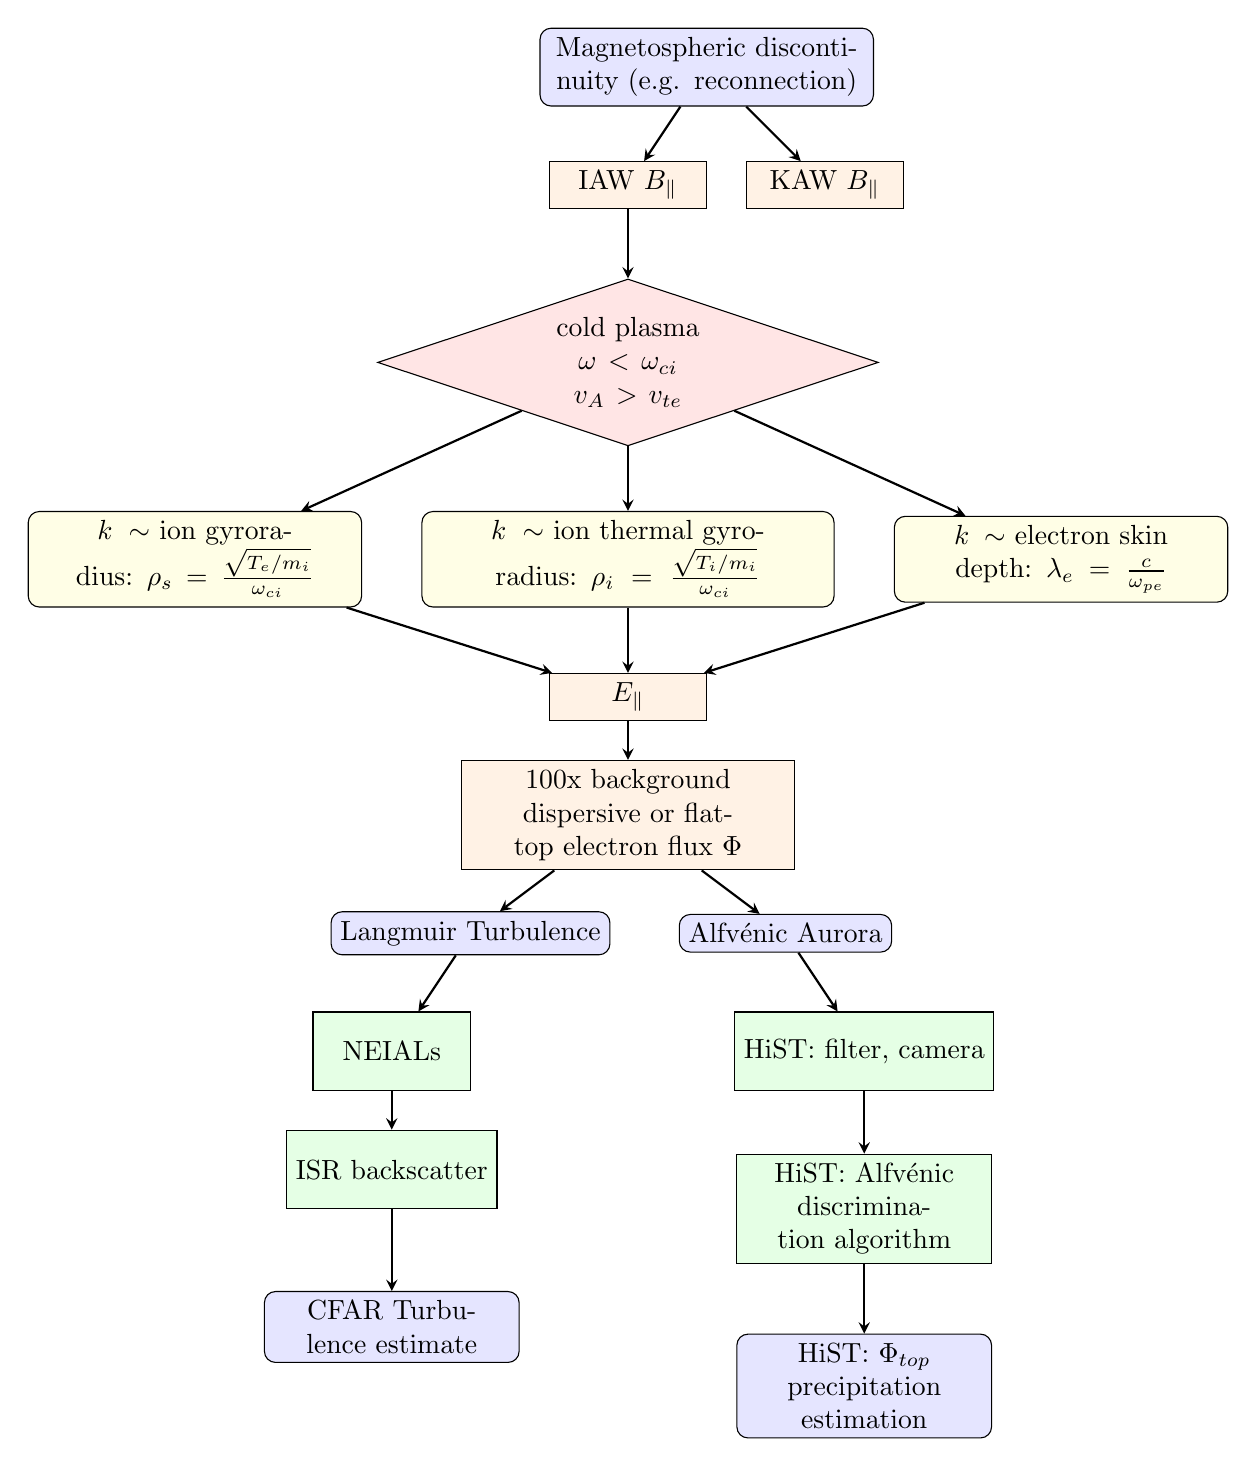
\begin{tikzpicture}[node distance=1.5cm, auto]
    
    \node (magdis) [startstop,text width=4cm] {Magnetospheric discontinuity (e.g. reconnection) \par };
       
    \node (iaw) [process, below of = magdis,xshift=-1 cm] {IAW $B_\parallel$ \par };
    
    \node (kaw) [process,right of = iaw,xshift=1 cm] {KAW $B_\parallel$ \par };
    
    \node (wl) [decision, below of=iaw,text width=2 cm,yshift=-0.75cm] { cold plasma  $\omega < \omega_{ci}$ $v_A > v_{te}$ \par };
    
    
    \node (iontherm) [estimate, below of=wl,yshift=-1 cm, text width=5cm]{ $k \sim$ ion thermal gyroradius: $ \rho_i = \frac{\sqrt{T_i/m_i}}{\omega_{ci}} $ \par};
    
    \node (iongyro) [estimate, left of=iontherm,xshift=-4cm, text width=4cm]{ $k \sim$ ion gyroradius: $ \rho_s = \frac{\sqrt{T_e/m_i}}{\omega_{ci}} $ \par};
    
    \node (eskin) [estimate, right of=iontherm,xshift=4cm,text width=4cm]{ $k \sim$ electron skin depth: $\lambda_e = \frac{c}{\omega_{pe}}$ \par};
    
    \node (accel) [process, below of=iontherm,yshift=-0.25cm]{$ E_\parallel$ \par};
    
    \node(eflux) [process,below of=accel,text width=4cm]{100x background dispersive or flat-top electron flux $\Phi$ \par};
    
    \node(lt) [startstop, below of=eflux,xshift=-2cm]{Langmuir Turbulence \par};
    
    \node(aurora) [startstop, below of=eflux,xshift=2cm]{Alfvénic Aurora \par};
    
    \node(neial) [compute,below of=lt,xshift=-1cm] {NEIALs \par};
    \node(isr) [compute,below of=neial]{ISR backscatter \par};
    \node(isrest)[startstop,below of=isr,text width=3cm,yshift=-.5cm]{CFAR Turbulence estimate \par};
    
    \node(hist)[compute,below of=aurora,xshift=1cm]{HiST: filter, camera};
    \node(det)[compute,below of=hist,text width=3cm,yshift=-.5cm]{HiST: Alfvénic discrimination algorithm};
    \node(est)[startstop,below of=det,text width=3cm,yshift=-.75cm]{HiST: $\Phi_{top}$ precipitation estimation};
    
    \draw[arrow] (magdis) -- (iaw);
    \draw[arrow] (magdis) -- (kaw);
    \draw[arrow] (iaw) -- (wl);
    \draw[arrow] (wl) -- (iongyro);
    \draw[arrow] (wl) -- (iontherm);
    \draw[arrow] (wl) -- (eskin);
    \draw[arrow] (iongyro) -- (accel);
    \draw[arrow] (iontherm) -- (accel);
    \draw[arrow] (eskin) -- (accel);
    \draw[arrow] (accel) -- (eflux);
    \draw[arrow] (eflux) -- (aurora);
    \draw[arrow] (eflux) -- (lt);
    
    \draw[arrow] (lt) -- (neial);
    \draw[arrow] (neial) -- (isr);
    \draw[arrow] (isr) -- (isrest);
    
    \draw[arrow] (aurora) -- (hist);
    \draw[arrow] (hist) -- (det);
    \draw[arrow] (det) -- (est);
    
    \end{tikzpicture}
    \caption{Block diagram of Alfvénic aurora acceleration mechanism and HiST observation.}
    \label{fig:alfvenblock}
\end{figure}
A key ground-observable characteristic of Alfvénic aurora is narrow arc width.
``Width'' describes spatial scale size in the dimension perpendicular to geomagnetic field $B$.
\citet{maggsdavis1968} noted that the lower observed limit of \unit[70]{m} arc width was instrumentally limited.
\citet{borovsky1993} noted that observations from contemporary ground-based auroral arc measurements continued to reveal arc widths less than \unit[100]{m}.
Alfvénic aurora are associated with a sudden large increase in flux of particles accelerated from a few eV to as much as \unit[10]{keV} \citep{chaston2003}.
Due to dispersion along the accelerated particle path, over several hundred milliseconds \citep{dahlgren2013} the characteristic energy $E_0$ will go from order \unit[10]{keV} to order \unit[100]{eV}.
A representative differential number flux for a DAW event is shown in Figure~\ref{fig:alfvenflux}.
\begin{figure}
    \includegraphics[width=0.9\columnwidth]{gfx/eflux}
    \caption{Evolution of characteristic energy $E_0$ from order \unit[10]{keV} to order \unit[100]{eV} occurs in \unit[100..1000]{ms} for DAW.
    In this plot, overall flux $Q_0$ is held constant.}
    \label{fig:alfvenflux}
\end{figure}
\textit{In situ} Freja measurements with \unit[32]{kHz} sampling rate \citep{stasiewicz2000} consistently showed plasma evacuations by roughly a factor of two near magnetic perturbations along $B_\parallel$ consistent with the presence of Alfvén waves.
Considering the \unit[7]{km/s} platform motion, the spectrograms of magnetic field point to $k_\perp \in [10,7000]$~m.
Freja also observed clear correlations \citep{stasiewicz2000} with turbulent magnetic field and suprathermal electron bursts ranging from \unit[100]{eV} to \unit[20]{keV} with particle fluxes of order 100 times over the background, and Poynting flux of $\unit[1..20]{mW/m^2}$.

The sampling cadence configuration of PFISR and the optical instruments for each experiment is given in Table~\ref{tab:cadence}.
These raw sample times are far faster than the minute cadence typically employed for plasma parameter estimation, yet those minute-long estimates break down in the face of these transient events.
We examine four types of events in turn: auroral breakup, splitting auroral arc, flaming auroral arc, and kinked arc with joint analysis of optical, spectral and radar features.


\FloatBarrier
\subsection{Breakup Auroral Arcs}\label{sec:breakup}
Highly dynamic events may combine several auroral morphologies, driven by diverse acceleration mechanisms, yielding multiple plasma turbulence types in close spatiotemporal proximity.
These events are difficult to interpret with instruments smearing in time by a factor of 100..1000 times greater than the ground-observable timescales.
It is also impractical to have a human manually initiating recording during extended observations.
This fact motivates the automatic Alfvénic aurora discrimination algorithms cited in section~\ref{sec:hist}.

A canonical example of such an event motivating the HiST system was the auroral breakup of March 23, 2007 shown in Figure~\ref{fig:20070323}.
\begin{figure}
    \noindent\includegraphics[width=0.9\columnwidth,trim=0 383 0 10,clip]{gfx/2007-03-23/2007-03-23}
    \vspace{0.1cm}
    
    % psd ion-line
    \includegraphics[width=0.3\columnwidth,trim=0 55 0 0]{gfx/2007-03-23/acfslice_alternatingcode2007-03-2311-20-08}
    \includegraphics[width=0.3\columnwidth,trim=0 55 0 0]{gfx/2007-03-23/acfslice_alternatingcode2007-03-2311-20-23}
    \includegraphics[width=0.3\columnwidth,trim=0 55 0 0]{gfx/2007-03-23/acfslice_alternatingcode2007-03-2311-20-39}
    
    \vspace{-0.5cm}
    \hspace{0.1cm}(f)\hspace{0.275\columnwidth}(g)\hspace{0.275\columnwidth}(h)
    \vspace{0.1cm}
    
    % psd plasma-line
    \includegraphics[width=0.45\columnwidth,trim=0 60 0 0]{gfx/2007-03-23/plasmaDOWNslice2007-03-2311-20-08}
    \includegraphics[width=0.45\columnwidth,trim=0 60 0 0]{gfx/2007-03-23/plasmaUPslice2007-03-2311-20-08}
    
    \vspace{-0.5cm}
    \hspace{0.5cm}(i)\hspace{0.425\columnwidth}(j)
    \vspace{0.5cm}
    
    \caption{Substorm breakup: highly dynamic aurora on 23 March 2007. 
        Low-altitude NEIALs observed corresponding to (a,c,f,i,j) with possible Farley-Buneman instability in the E-region. 
        Streaming upflow corresponding to (d,h).
    Strong Langmuir turbulence corresponding to (c,f,g). }\label{fig:20070323}
\end{figure}
The PF-DMSP spectra ratio $I_{6300}/I_{4278}$ in Figure~\ref{fig:mspratio0323} dips as low as 0.02 during the breakup, indicating a large flux with $E_0 > \unit[10]{keV}$ according to \citet{rees1974}.
\begin{sidewaysfigure}\centering
    \includegraphics[width=0.85\linewidth]{gfx/2007-03-23/msp-ratio}
    \caption{PF-DMSP spectral ratio breakup event 2007 March 23 11:22 UTC.
        The ratio $I_{6300}/I_{4278}$ dips as low as 0.02 during the breakup, indicating a large flux with $E_0 > \unit[10]{keV}$ according to \citet{rees1974}.}
    \label{fig:mspratio0323}
\end{sidewaysfigure}
The $I_{5577}/I_{4278}$ in Figure~\ref{fig:mspratio0323-5577} dips as low as 1 during the breakup, also indicating a large flux with $E_0 > \unit[10]{keV}$ according to \citet{rees1974}.
\begin{sidewaysfigure}\centering
    \includegraphics[width=0.85\linewidth]{gfx/2007-03-23/msp-ratio-5577}
    \caption{PF-DMSP spectral ratio breakup event 2007 March 23 11:22 UTC.
        The ratio $I_{5577}/I_{4278}$ dips as low as 1 during the breakup, indicating a large flux with $E_0 > \unit[10]{keV}$ according to \citet{rees1974}.}
    \label{fig:mspratio0323-5577}
\end{sidewaysfigure}
The GIMA magnetometers data surrounding this event is shown in Figure~\ref{fig:20070323mag}, with the expected strong perturbation near the event time.
\begin{figure}
    \includegraphics[width=\columnwidth]{gfx/2007-03-23/mag}
    \caption{Strong B-field perturbance due to substorm on 2007-03-23 near 11:20 UTC.}
    \label{fig:20070323mag}
\end{figure}

This was an exceptionally intense breakup event.
This magnificent substorm breakup had splitting arcs embedded in the wildly dynamic behavior captured by PFISR and a single BG3-filtered EMCCD camera. 
This event has been analyzed in detail by \citet{semeter2008,akbari2012}.


\subsection{Splitting Auroral Arcs}\label{sec:split}
One of the ground-observable optical manifestations of a DAW event are bifurcating ``shedding'' or ``splitting'' arcs, which have a pattern of one or more spatiotemporal leaves folding off of the main arc. 
During the shedding event of Figures~\ref{fig:20130414T0854a}-\ref{fig:20130414T0854b}, PFISR power in the magnetic zenith beam (represented by a red circle in Figure~\ref{fig:20130414T0854a}(a-d)) is enhanced by over \unit[25]{dB} in the F-region ionosphere above the bifurcation zone.
\begin{sidewaysfigure}\noindent

    \includegraphics[width=\columnwidth,trim=0 680 0 50,clip]{gfx/2013-04-14T0854/2013-04-14T0854}\\
    
    \vspace{-1.175cm}
    \hspace{1.35cm}{\color{white}(a) 08:54:16}
    \hspace{2.1cm}{\color{white}(b) 08:54:21}
    \hspace{2.15cm}{\color{white}(c) 08:54:26}
    \hspace{2.15cm}{\color{white}(d) 08:54:31}
    \vspace{0.5cm}
    
    % backscatter
    \begin{center}
    \includegraphics[width=0.9\columnwidth,trim=10 0 0 185,clip]{gfx/2013-04-14T0854/power_longpulse2013-04-1408-54}\\
    \end{center}
    
    \vspace{-1.5cm}
    (e) 
    \vspace{.5cm}
      
    \caption{Splitting auroral arc sequence at PFISR, April 14, 2013. 
        (a) beginning of plasma turbulence bursts.
        (b) F-region ionization increasing nearly \unit[30]{dB} above background. 
        The turbulence fades in (c), enhancing to even greater intensity in (d) for ten seconds.
        (e) backscattered ISR power.}
    \label{fig:20130414T0854a}
\end{sidewaysfigure} 

\begin{figure}\noindent
	   % psd ion-line 
	\includegraphics[width=0.425\columnwidth]{gfx/2013-04-14T0854/acfslice_longpulse2013-04-1408-54-16}
	\includegraphics[width=0.425\columnwidth]{gfx/2013-04-14T0854/acfslice_longpulse2013-04-1408-54-31}\\
	
	\vspace{-1.5cm}
	\hspace{0.0cm}(a)\hspace{0.4\columnwidth}(b)
	\vspace{0.3cm}
	
	% down-shift
	\includegraphics[width=0.425\columnwidth,trim=0 50 0 0]{gfx/2013-04-14T0854/plasmaDOWNslice2013-04-1408-54-16}
	\includegraphics[width=0.425\columnwidth,trim=0 50 0 0]{gfx/2013-04-14T0854/plasmaUPslice2013-04-1408-54-16}\\
	
	\vspace{-1.2cm}
	\hspace{0.0cm}(c)\hspace{0.4\columnwidth}(d)
	\vspace{0.3cm}
	
	% up-shift
	\includegraphics[width=0.425\columnwidth,trim=0 50 0 0]{gfx/2013-04-14T0854/plasmaDOWNslice2013-04-1408-54-31}
	\includegraphics[width=0.425\columnwidth,trim=0 50 0 0]{gfx/2013-04-14T0854/plasmaUPslice2013-04-1408-54-31}\\
	
	\vspace{-1.2cm}
	\hspace{0.0cm}(e)\hspace{0.4\columnwidth}(f)
	\vspace{0.3cm}
	
	\caption{Splitting auroral arc sequence at PFISR, April 14, 2013.
		(a,b) backscattered power related to (a-c) and (d) respectively.
		(c,d) down- and up-shifted plasma line enhancements corresponding to Figure~\ref{fig:20130414T0854a}(a-c).
		(e,f) down- and up-shifted plasma line enhancements corresponding to Figure~\ref{fig:20130414T0854a}(d).}
	\label{fig:20130414T0854b}
\end{figure}
On the night of April 14, 2013, several instruments with diverse observing modalities were active in the vicinity of PFRR, as depicted in Figure~\ref{fig:sitemap}. 
PFISR and DASC are co-located, so the center of the PFISR beams in the image can be taken as approximately constant.
The GIMA magnetometer data is shown in Figure~\ref{fig:gima0854}, showing the usual southward IMF in the time vicinity of the splitting arc.
\begin{figure}
	\includegraphics[width=\columnwidth]{gfx/2013-04-14T0854/mag}
	\caption{PFRR GIMA magnetometer data for 2013-04-14 showing evidence of southward IMF in time vicinity of splitting arc.}
	\label{fig:gima0854}
\end{figure}


Observe in Figure~\ref{fig:20130414T0854b}(c-f) that only the plasma line spectra for 08:54:16 and 08:54:31 UT show prominent reflections from plasma turbulence.
The rest of the plasma line spectra near this time looks much like the 08:54:45 data.
%In contrast, the ion line spectrum in Figure~\ref{fig:20130414T0854}(f,g,h) still shows the turbulence effects at 08:54:45, so an earlier frame at 08:54:02 UT is included to show the non-turbulent ion line spectra.
%A movie sequence for this event is available in the Supplemental Materials for this article.
We integrate the received ISR power over the NEIALs altitude range and plot this integrated measurement with the HiST optical data. 
It is initially apparent from comparing Figure~\ref{fig:20130414T0854a}(a-d) with Figure~\ref{fig:20130414T0854a}(e) that the highest SNR bursts come from the times when the magnetic zenith ISR beam is over a region of optically ``shedding'' arcs.
Figure~\ref{fig:20130414T0854a}(a) depicts a typical dispersive Alfvén wave auroral scene. 
The red circle denotes local magnetic zenith. 
Observe the fine spatial structure along the $B_\perp$ direction. 
Figure~\ref{fig:shedintion}(b) shows the plasma line summed over altitudes from \unit[200..350]{km}.
Figure~\ref{fig:20130414T0854b}(a,b) shows the ion line PSD during the time of this shedding auroral event--observe the ``flat top'' characteristic of the spectrum seen only during NEIALs.

Turning to optical spectral information, the PF-DMSP data in Figure~\ref{fig:shedratio0854}(a-b) is used to compare \unit[427.8]{nm} intensity from N$_2^+$ $I_{427.8}$ with prompt OI emissions at \unit[630.0]{nm} $I_{630.0}$.
This ratio in Figure~\ref{fig:shedratio0854}(c) shows that just before and during the splitting arc, $I_{427.8}$ is nearly twice as strong as $I_{630.0}$. 
\begin{figure}
    \includegraphics[width=\columnwidth,trim=3 3 3 3,clip]{gfx/2013-04-14T0854/MSPintensityratio}
    \caption{PF-DMSP (a) $I_{630.0}$ and (b) $I_{427.8}$ emission intensity with (c) $I_{630.0}/I_{427.8}$ emission intensity ratio at 08:54 UT during the 14 April 2013 substorm. Golden dashed lines refer to approximate elevation FOV of HiST cameras.}\label{fig:shedratio0854}
\end{figure}
After the splitting event completes, the \unit[630.0]{nm} line once again dominates $I_{427.8}$ by a factor of 1.5 to 3.5 as was also the case before the splitting began.
Figure~\ref{fig:shedratioplot0854} provides an alternative view of $I_{630.0}$/$I_{427.8}$.
\begin{figure}
    \includegraphics[width=0.9\columnwidth]{gfx/2013-04-14T0854/msp_ratio}
    \caption{PF-DMSP ratio of $I_{630.0}/I_{427.8}$ emission intensity ratio with one line plot per time. Observe that high energy beam (indicated by lowest ratio at 08:54:10) does not immediately lead to splitting arc. It takes about 10 seconds for visible arc splitting to occur. Golden dashed lines refer to approximate elevation FOV of HiST cameras.}
    \label{fig:shedratioplot0854}
\end{figure}
%These measurements are within the typical range for $I_{630.0}$ and $I_{427.8}$~\citep{Dashkevich2006}.
From \citet{rees1974}, at 08:54:10 UTC at the magnetic zenith angle of $102.5^\circ$ elevation from north, $I_{630.0}/I_{427.8} \sim 0.6$, corresponding to a characteristic energy of \unit[1.6]{keV} for the assumptions on neutral composition and brightness observed.

Historical work has often relied on spectrometer readings for estimates of characteristic energy $E_0$, represented in Figure~\ref{fig:alfvenflux} as the high-energy ``bump''.
Historically these measurements had cadences of several seconds, and obviously lacked a sense of the auroral morphology.
As the extensive literature referenced throughout this paper has noted, quantitative correlation of auroral spatio-temporal evolution with plasma turbulence requires an FOV of several degrees about magnetic zenith with at least 40 frames/s sampling, and with filtering sufficient to remove the blur of metastable emissions \citep{hirsch2016}.
The tomography data inversion exemplified in Figures~\ref{fig:histfwd} and \ref{fig:histest} is an example of the new capabilities afforded by HiST for such applications.
\begin{sidewaysfigure}\centering
    \includegraphics[width=0.9\columnwidth]{gfx/fwd0}
    \caption{Forward model of aurora for HiST two-camera deployment at PFRR. Splitting arc is simulated. 
    	Panel (a) shows ground-observed optical intensity after filtering and wavelength-dependent atmospheric attenuation. 
    	(b) shows the auroral optical volume emission rate vs. $B_\perp$. 
    	(c) shows the unobservable primary electron differential number flux at the ``top'' of the ionosphere, this is the quantity the HiST system estimates with high spatiotemporal resolution.}\label{fig:histfwd}
\end{sidewaysfigure}
\begin{sidewaysfigure}\centering
    \includegraphics[width=0.75\columnwidth]{gfx/est0}
    \caption{Data inversion for forward modeled HiST two-camera deployment at PFRR. Splitting arc is simulated as in Figure~\ref{fig:histfwd} and precipitation estimated. Panel (a) shows ground-observed and estimated optical intensity after filtering and wavelength-dependent atmospheric attenuation. (b) shows the estimated auroral optical volume emission rate vs. $B_\perp$. (c) shows the estimated primary electron differential number flux at the ``top'' of the ionosphere. (d) shows a 1-D vertical cut of volume emission rate for the two arcs, forward model and estimated. (e) shows a 1-D cut in $B_\perp$ for each arc, forward model and estimated differential number flux.}\label{fig:histest}
\end{sidewaysfigure}

\subsection{Flaming auroral arcs}\label{sec:fusflame}
Flaming aurora manifests as rapidly increasing peak brightness altitude.
The effect can have an appearance like the rapidly rising flames of a campfire, leading to the name for this auroral morphology.
The driving factor behind flaming aurora is dispersive Alfvén waves.
The high energy precipitating particles arrive first in the auroral altitudes of the ionosphere, followed $\sim \unit[100]{ms}$ later by the lower energy particles.

An example flaming auroral arc occurred at PFISR on March 1, 2011 near 10:06 UTC.
Figure~\ref{fig:20110301a}(a) shows pre-Alfvénic arc configuration.
F-region irregularities starting below \unit[300]{km} and rising up to \unit[600]{km} within two seconds are observed in Figure~\ref{fig:20110301a}(b) ISR power with the arrival of high-energy dispersive Alfvénic particles.
\unit[400]{ms} later in Figure~\ref{fig:20110301a}(c), the low-energy Alfvénic flux dominates as the apparent peak altitude of prompt emissions rises rapidly.
Figure~\ref{fig:20110301b}(a) shows the ion-line during the NEIAL altitude climb, with (g) after the NEIAL rose to a more steady altitude.
A few seconds later in Figure~\ref{fig:20110301a}(d), the Alfvénic particle packet has vanished.
Figure~\ref{fig:20110301b}(c) shows the ion-line spectrum without NEIALs present.
Observe that two more NEIAL events occurred before and after the video, but due to the human-initiated record cycle, they were not recorded with video.
\begin{sidewaysfigure}\centering
    % Video
    \includegraphics[width=0.19\columnwidth,trim=30 0 200 0,clip]{gfx/2011-03-01/2040}
    \includegraphics[width=0.261\columnwidth,trim=30 0 60 0,clip]{gfx/2011-03-01/6440}
    \includegraphics[width=0.261\columnwidth,trim=30 0 60 0,clip]{gfx/2011-03-01/6840}
    \includegraphics[width=0.261\columnwidth,trim=30 0 60 0,clip]{gfx/2011-03-01/10440}
    % Power
    \includegraphics[width=\columnwidth,trim=0 50 0 0]{gfx/2011-03-01/power_longpulse2011-03-0110-06-00}\\
    {\large(e)}
    \vspace{0.1cm}

    \caption{Flaming auroral arc sequence at PFISR on March 1, 2011, 10:06 UTC.
        (a) shows pre-Alfvénic arc configuration.
        (b) F-region irregularities are observed in the ISR power (e) with the arrival of high-energy DAW accelerated electron.
        (c) \unit[400]{ms} later, the low-energy Alfvénic flux dominates as the apparent peak altitude of prompt emissions rises rapidly.
        (d) the Alfvénic particle packet has vanished.
        (e) ISR backscatter showing three NEIAL events in series--video only available for middle event.}
    \label{fig:20110301a}
\end{sidewaysfigure}

\begin{figure}\centering
    % Psd
    \includegraphics[width=0.5\columnwidth,trim=0 50 0 0]{gfx/2011-03-01/acfslice_longpulse2011-03-0110-06-11}

    \vspace{-1cm}(a)
    \vspace{1cm}

    \includegraphics[width=0.5\columnwidth,trim=0 50 0 0]{gfx/2011-03-01/acfslice_longpulse2011-03-0110-06-17}

    \vspace{-1cm}(b)
    \vspace{1cm}

    \includegraphics[width=0.5\columnwidth,trim=0 50 0 0]{gfx/2011-03-01/acfslice_longpulse2011-03-0110-06-28}

    \vspace{-1cm}(c)
    \vspace{1cm}

	%(a)\hspace{0.275\columnwidth}(b)\hspace{0.275\columnwidth}(c)

	\caption{Flaming auroral arc sequence at PFISR on March 1, 2011.
    (a,b) show enhanced negative frequency shift ion-acoustic line.
    (c) shows normal ion-acoustic line.}
    \label{fig:20110301b}
\end{figure}

Only a single high-speed sCMOS was running at 30 frames/s, in burst recording mode of several seconds each manual record start.
Context for the event is provided by PF-DMSP in Figure~\ref{fig:msp20110301} and GIMA in Figure~\ref{fig:mag20110301}.
\begin{figure}\centering
    \includegraphics[width=\columnwidth]{gfx/2011-03-01/mag}
    \caption{Quiet conditions before the flaming auroral event are perturbed during the 2011-03-01 substorm.}
    \label{fig:mag20110301}
\end{figure}
The PF-DMSP spectrum of Figure~\ref{fig:msp20110301} had $I_{555.7}$ and $I_{427.8}$ available.
\begin{figure}\centering
    \includegraphics[width=\columnwidth]{gfx/2011-03-01/msp_ratio}
    \caption{PF-DMSP (a) $I_{555.7}$ and (b) $I_{427.8}$ with ratio (c) $I_{555.7} / I_{427.8}$. Around 10:06 and 10:11 UTC  intensifications near magnetic zenith indicates large increase in characteristic energy.}
    \label{fig:msp20110301}
\end{figure}
According to \citet{rees1974}, the magnetic zenith energies are on the order of \unit[5..10]{keV} during this event.
The PF-DMSP data is highly smeared in time across this event.
\citet{dahlgren2013} provided estimates using assumptions on the starting altitude of the flaming feature in a single-camera data inversion.
HiST was designed to study this type of event, with long-term automated recording so that events are not missed and the precipitation energy dynamics can be examined in more quantitative detail.

\FloatBarrier
\subsection{Kinked auroral arc}\label{sec:kink}
Auroral arcs with folds or kinks originate with magnetospheric configurations that are non-dispersive in nature.
Such disturbances also drive auroral vortices and vortex streets.
A striking example of a kinked auroral arc is shown in Figure~\ref{fig:20130414T0826}.
\begin{sidewaysfigure}\centering
    \noindent\includegraphics[width=\columnwidth,trim=15 697 25 0,clip]{gfx/2013-04-14T0826/2013-04-14T0826}

    \hspace{1.1cm}(a) 08:26:07.400 UT 
    \hspace{1.25cm}(b) 08:26:08.000 UT
    \hspace{1.1cm}(c) 08:26:08.100 UT
    \hspace{1.1cm}(d) 08:26:12.000 UT
    
    \caption{Narrow kinking and translating arcs at PFISR, ca. 08:26:10 UTC on April 14, 2013. 
          No coherent echoes detected in ion line, plasma line, or power spectral density.}
    %Two satellites cross through the field of view nearly orthogonally at 08:24:18 UTC.
    \label{fig:20130414T0826}
\end{sidewaysfigure}
A substorm is indicated as the initiator of the perturbation based on the southward turning IMF reflected in sharp negative excursion at 08:25 UTC as shown in Figure~\ref{fig:mag0826}.
\begin{figure}\centering
    \includegraphics[width=\columnwidth]{gfx/2013-04-14T0826/mag}
    \caption{GIMA PFRR data showing geomagnetic field reversal near 08:25 UTC.}
    \label{fig:mag0826}
\end{figure}
A likely driver for this arc structure is an inverted-V acceleration region.
%As observed with HiST the auroral spectrum including the lines of Figure~\ref{fig:msp0826} is passed through the HiST BG3 filter, yielding $I_{557.7} \sim 0.01 \times I_{427.8}$.
The $I_{427.8}$ intensity suggests monoenergetic several keV electron beam configuration.
\begin{figure}
    \includegraphics[width=\columnwidth]{gfx/2013-04-14T0826/msp_spectra}
    \caption{PF-DMSP spectrum showing strong $I_{427.8}$, suggesting monoenergetic beam of several keV driving kinked arc near 08:26 UTC.}\label{fig:msp0826}
\end{figure}
Monoenergetic inverted-V accelerated electron differential number flux in the several keV range is the most likely candidate for generating this kinked aurora.
\section{Discussion and Conclusions}\label{sec:disc}
In-situ measurements obtained from sounding rockets have long established that intense Langmuir waves with amplitudes approaching \unit[1.2]{V/m} are common features of the auroral ionosphere. 
Langmuir waves are observed propagating nearly parallel to $B$ and occur in bursts with durations of hundreds of milliseconds \citep{mcfadden1986,boehm1984,ergun1999a,ergun1999b}.
Freja observations confirm that Langmuir waves are the strongest electrostatic waves at altitudes $\sim \unit[1500]{km}$ \citep{stasiewicz1996}.
Such Langmuir waves have been suggested to play an important role in the auroral ionosphere energy flow chain, facilitating energy transfer from AW to the bulk plasma \citep{stasiewicz1996}.

Although observation of intense Langmuir waves in the ionosphere is not a new finding, the significance of ISR detected Langmuir turbulence lies in the specific wavenumber at which ISR-detectable wave activities are enhanced. 
The detection of Langmuir waves at relatively high wave numbers: $k \sim \unit[19]{m^{-1}}$ for PFISR and $k \sim \unit[39]{m^{-1}}$  for EISCAT puts constraints on the dynamics of interactions and/or on the characteristics of the underlying energy source for the enhanced waves \citep{akbari2014}.
Furthermore, there seems to be discrepancies between ISR and in-situ observations:
\begin{enumerate}
    \item \textit{in situ} measurements suggest that Langmuir turbulence should be commonly observed at altitudes above 600~km, whereas the ISR echoes are seen consistently at the F-region peak around 250-300 km.
    \item ISR measurements suggest that the intense Langmuir waves generate a well-developed turbulence which leads to caviton formation and collapse, whereas signatures of caviton formation have been completely missing in the \textit{in situ} measurement literature, with the exception of the inconclusive results of \citet{boehm1984}.
    \item \textit{In situ} measurements have shown that the enhanced Langmuir waves at higher altitudes are rather monochromatic \citep{ergun1999a,ergun1999b}. 
\end{enumerate}

A portion of the apparent inconsistencies between ISR and \textit{in situ} measurements may naturally arise from the different dynamics of beam-plasma interactions expected at different altitudes (i.e. \unit[250..300]{km} versus $>\unit[600]{km}$).
However, one should be cautious about drawing a definite conclusion that the processes underlying the radar echoes are just a low-altitude extension of the beam-plasma interactions long known from \textit{in situ} measurements.

An aspect of the ISR observations that bears discussion is the source of free energy underlying the detected turbulence.
In natural plasmas a common mechanism for intensification of Langmuir waves is the bump-on-tail instability (or inverse Landau damping) which operates upon the existence of a bump (positive slope) on the reduced (one-dimensional) electron velocity distribution function. 
This bump often represents the existence of an additional population of electrons on top of the bulk electrons. 
This population could be locally produced via acceleration or energization of a portion of the local electrons, or it could consist of electrons traveling to the observer in the form of electron beams. 
In the lower ionosphere and in the absence of any known local acceleration mechanism, a bump on the distribution function may directly arise from:
\begin{enumerate}
    \item the auroral magnetospheric-origin electron beams that are accelerated at high altitudes and propagate to the lower ionosphere (with energies of hundreds of eV to a few keV or more)
    \item the secondary electron population (with energies of a few eV to $\sim \unit[100]{eV}$) that emerges as a result of collisional interactions of the primary auroral electrons with the Earth's neutral atmosphere.
\end{enumerate}
In the former case, it is crucial to make a distinction between the electron beams accelerated by inertial AW and the inverted-V electron beams accelerated by quasi-static parallel electric fields. 

Detection of Langmuir waves in the ISR plasma-line channels enables the determination of the phase velocity $v_\varphi=\omega / k$ of the Langmuir waves and consequently the energy of the electrons directly exchanging energy with the waves. 
For PFISR observations, this energy is $\sim \unit[5]{eV}$, which falls in the energy range of secondary electrons. 
This may suggest that the secondary electrons provide the energy for the turbulence. 
Secondary electrons are known to be responsible for intensification of Langmuir waves in the E-region of the auroral ionosphere \citep{nilsson1996}. 
Langmuir wave intensification in such cases is associated with the presence of a bump, itself associated with the absorption cross-section of $N_2$, in the three-dimensional distribution function which results in reduction of Landau damping and increase in the Čerenkov emission rate. 
However, numerical modelings \citep{nilsson1996} have show that this bump appears over a broad range of pitch angles and is nearly isotropic at lower altitudes of the E-region and do not produce a bump in the reduced (one-dimensional) distribution function. 
As such, the plasma remains stable and the intensification of Langmuir waves is limited. 
At higher altitudes, the secondary electron spectra further deviate from isotropic; however, the pump becomes less pronounced due to the change in the neutral gas composition.

In summary, although secondary electrons have been suggested to cause plasma instabilities involving wave modes propagating nearly perpendicular to the magnetic field lines \citep{basu1982,jasperse2013}, are generally considered stable with respect to Langmuir waves. 
An additional evidence against the secondary electrons as the energy source for the F region Langmuir turbulence echoes, exists in the ISR data; where no correlation between the E region ionization (which is proportional to the secondary electron production rate) and the Langmuir turbulence echoes is found \citep{akbari2013}. 
It is also worth mentioning that the presence of secondary electrons with power law-like distributions, not only does not lead to instability, but instead significantly weakens the turbulence via introducing enhanced Landau damping to Langmuir waves \citep{newman1994linear,newman1994nonlinear,akbari2015}. 

The problem regarding the primary energetic auroral electrons as the source of energy for the turbulence underlying the radar echoes is that the Langmuir waves that are directly in energy exchange with such energetic electrons have wave numbers far below the detecting wave numbers of the existing incoherent scatter radars and, as such are undetectable.
Assuming that the parametric decay of Langmuir waves is the main product of the beam-plasma interactions at the observation altitudes, the energy transfers to yet smaller wave numbers, via a cascade of PDIs, and further away from the radar wavenumber. 
However, it has been shown that a well developed Langmuir turbulence does transfer a small fraction of the input energy to higher wave numbers via processes such as the caviton collapse or three-wave coalescence-like interactions \citep{akbari2014,akbari2015}, and that these could be the origin of the observed ISR echoes. 
Therefore, the possibility that the primary auroral electron beams are the direct source of the turbulence may not be ruled out.

It is necessary to make a distinction between the two types of electron beams that are commonly observed in the auroral ionosphere, i.e. the inverted-V electron beams and the field-aligned electron bursts. 
The inverted-V electron beams are produced by acceleration of warm plasma sheet electrons via quasi-static parallel electric fields at the earth acceleration region. 
It is possible for the inverted V electron beams to produce a positive slope in the one-dimensional distribution function at high altitudes close to the acceleration region. 
However, in short time scales and before the beams have the chance to travel long distances, the self-generated plasma waves quickly plateau the positive slope via  quasi-linear diffusion \citep{sanbonmatsu2001}, rapidly stabilizing the distribution. 
In addition to the quasilinear diffusion, while traveling from the acceleration region toward the ionosphere, the inverted-V electron beams become subject to adiabatic evolution under the converging magnetic field limes. 
As a result of the magnetic mirror force, the field-aligned beam diffuses toward oblique and perpendicular directions \citep{maggs1981}, which although leading to intensification of oblique propagating wave modes such as the upper-hybrid and whistler modes \citep{maggs1978,kaufmann1980,maggs1981}, further stabilize the distribution against Langmuir waves. 

Sounding rocket measurements of the three-dimensional electron velocity distributions at F-region altitudes, have consistently shown that the inverted-V electron beams often have a broad, nearly isotropic plateau that despite having a positive slope in the three-dimensional distribution function, does not produce a positive slope in the reduced (one-dimensional) distribution function in near parallel directions \citep{kaufmann1978,kaufmann1980,mcfadden1986}.
Such distributions are, therefore, stable against Langmuir turbulence. 
This general rule, however, may not be correct universally. 
From the experimental point of view, given the low temporal resolution of the electron velocity distribution function measurements, the existence of transient positive slopes in time scales shorter than the measurement resolutions may not be completely ruled out. 
Also from the theoretical point of view, a number of linear (wave refraction) \citep{maggs1978} and nonlinear (parametric type instabilities) \citep{papad1974} mechanisms have been suggested to be able to limit the growth of the beam-generated electrostatic waves and, consequently, limit the quasi-linear flattening of the beam, ultimately enabling the beam to maintain its unstable features while traveling down to the F-region altitudes. 
While such considerations can not be completely ruled out, a final evidence against the inverted-V electron beams as the source of turbulence underlying the ISR echoes, lies in the ISR data itself, where no correlation between the E-region ionization enhancements (the signature of energetic electron precipitation) and the turbulence echoes are found.

In contrast to inverted-V electron beams, field-aligned electron bursts produced by acceleration of cold ionospheric electrons via parallel electric field of inertial Alfvén waves \citep{kletzing2001,semeter2008} have characteristics that make them suitable candidates as the energy source for Langmuir wave enhancement at various altitudes. 
An important characteristic of the field-aligned bursts is their velocity dispersion, where the characteristic energy of the beam decreases from a few keV to $\sim\unit[100]{eV}$ over a period of $\sim \unit[100]{ms}$ (for a description of field-aligned bursts see \citet{mcfadden1987}). 
This dispersive behavior plays a major role in maintaining the beam distribution by continuously reproducing the positive slope of the distribution function, once flattened by the quasilinear diffusion, enabling the beam to remain unstable as it travels deep into the ionosphere \citep{ergun1993,sanbonmatsu2001}. 
This same behavior has been studied in the context of Langmuir wave enhancement in the solar wind and the type III radio bursts \citep{muschietti1990}. 

\textit{In situ} measurements obtained with sounding rockets have long established the connection between intense Langmuir waves in the auroral ionosphere and dispersive field-aligned electron bursts \citep{ergun1999a,stasiewicz1996}. 
Intense Langmuir waves observed \textit{in situ} are seen to undergo various non-linear interactions \citep{boehm1987,gough1990,ergun1999b}.
The association of:
\begin{enumerate}
    \item intense Langmuir waves with ISR Langmuir turbulence echoes
    \item dispersive Alfvénic accelerated electron beams with the source of energy underlying the echoes
\end{enumerate}  
are not obvious conclusions due to a number of discrepancies between the in-situ and ISR observations. 
Making such a connection, therefore, requires additional evidence as provided in this chapter from the joint HiST-PFISR observations.
Using the events presented in this paper and supplemental material, Table \ref{tab:events} collects the evidence for Alfvénic arcs corresponding to NEIALs.
\begin{sidewaystable}\centering
    \caption{Morphologies of events detailed in the paper and supplemental material. SLT=Strong Langmuir Turbulence}
    \label{tab:events}
    \begin{tabular}{lllll}
        \toprule
        Event Time [UT] & Aurora Morphology & ISR Morphology & Plasma Morphology & Figure \\
        \midrule
%        2007-03-18 & translating frozen-in & TODO & TODO & \\ % waiting SRI data
        2007-03-23 & splitting, flaming & 30 dB SNR ion line & SLT & \\
        2011-03-01 10:06 & flaming & $\Uparrow30$ dB ion line & Streaming upflow & \ref{fig:20110301a}, \ref{fig:20110301b} \\
%        2011-03-02 & & &  & \\
%        2012-11-07 & & & & \\
%        2013-04-01 & & & & \\
%        2013-04-04 & & & & \\
%        2013-04-07 & & & & \\
%        2013-04-11 & & & & \\
        2013-04-14 08:26 & Kinked, vortical & quiet & Thermal & \ref{fig:20130414T0826} \\
        2013-04-14 08:54 & Splitting/shedding & $\Uparrow30$ dB ion \& plasma lines & SLT & \ref{fig:20130414T0854a}, \ref{fig:20130414T0854b} \\
%        2013-04-14 09:27 & dark patches and flickering & quiet & Thermal & \ref{fig:20130414T0927}\\
%        2013-04-20 & & & & \\
%        2013-04-23 & & & & \\
%        2013-04-26 & & & & \\
%        2013-05-01 & & & & \\
        \bottomrule
    \end{tabular}
\end{sidewaystable}
The initial observations of the limited set of aurora and ISR turbulence presented suggests the following correspondence:
\begin{enumerate}
    \item inverted-V $\impliedby$ kinked aurora (Figure~\ref{fig:cartoonmorph}(a))
    \item strong Langmuir turbulence (F region) $\leftrightarrows$ splitting aurora (Figure~\ref{fig:cartoonmorph}(b))
    \item streaming upflow ($> 600$~km altitude)  $\leftrightarrows$ flaming aurora (Figure~\ref{fig:cartoonmorph}(c))
    
\end{enumerate}

\subsection{Future experimental configuration}\label{sec:future}
Using the BG3-filtered broadband prompt emission lines and bands captured by HiST cameras \citep{hirsch2016}, estimates of primary electron differential number flux with time scales fast enough to capture DAW behavior can be imaged and quantified.
Since the imaging chip provides a weighted sum of all emissions passing through the BG3 filter, spectral information is lost.
Existing spectrometers and hyper-spectral imagers \citep{goenka2016} typically have frame rates on the order of seconds to minutes.
The latest generation of EMCCD technology has $1024 \times 1024$ pixels at \unit[25]{fps}, nearly as fast as HiST imagers. 
A spectrograph is being tested for field deployment next year, colocated with HiST and with a similar FOV to resolve specific auroral emission lines. 
This additional data will help quantify the chemistry responsible for a discrete arc viewed by HiST, yielding further insights into the kinetics responsible for NEIALs.\cleardoublepage

\chapter{Conclusions and Future Work}
\label{chapter:Conclusions}
\thispagestyle{myheadings}
\graphicspath{{Concl/Figures/}}

\setlength{\epigraphwidth}{0.85\textwidth}
\epigraph{To the astronomer, after the celestial body has disappeared from his view, his main work starts.}{Gauss 1839 as translated by \citet{gauss1839}}

This dissertation presents the evolution of auroral morphology observations from antiquity and particularly from 1900 through the critical advances made by the dissertation work.
In particular, the advances in personal computing technology of the past decade were vital to enabling frame rates $\gg \unit[10]{fps}$ for more than five seconds at a manual push as discussed in chapter~\ref{chapter:inst}.
More importantly, the ability to sustain \unit[20]{ms} video cadence for months of unattended operation was developed in chapter~\ref{chapter:discrim}.
The instrumental and algorithm advancements by this dissertation work allow researchers to ``set and forget'' their cameras, allowing the capture of rare and infrequent auroral and meteor events and other as yet poorly characterized phenomena.
This may someday help solve new problems such as the theorized particle acceleration due to inertial Alfvén resonators and distinguish between the numerous inertial Alfvén wave modes via optical emissions due to the particles accelerated by the waves.

This dissertation presents work that unlocked several vital capabilities for recording, curating and processing into science quantities such high speed auroral data.
In chapter~\ref{chapter:discrim}, the ability to discriminate spatiotemporally fine-scale aurora from other types of aurora was demonstrated, eliminating the vast majority of auroral video recorded.
From the video segments that remained, in chapter~\ref{chapter:sim} a model-based iterative reconstruction algorithm incorporating a physics based electron penetration model of the ionosphere connected camera to radar data in joint ISR-Optical analysis and characterization of driving forces behind particular dynamic auroral spatiotemporal morphologies.
Chapter~\ref{chapter:fusion} presented real data inversions for HiST in light of ISR data, coming up with a joint quantitative solution based on high speed data from both instruments.

The algorithms created are immediately available to the public via Github and have already been used by other geoscience researchers studying auroral and other phenomenon. 
Algorithmic and science contributions from other geoscientists have already occurred with the Fortran and Python code developed during this dissertation.
Stable versions of the code are archived at Zenodo and assigned DOI for scholarly archival purposes.
As funding and time permit, the instruments and algorithms will be used and expanded for future projects.

A corollary to the dissertation work has been Michael Hirsch's outreach and advocacy at the state and federal legislatures in support of geoscience and geospace research.
The number of constituent phone calls, letters and emails legislative offices receive concerning the priority of basic science is said by their office staff to be nearly nil.
Taking a PiRadar prototype to Capitol Hill, where numerous US Senators and Representatives have Ph.D. staffers to assist the Members in their legislative and policy decisions engendered significant interest.
In reviewing the historical geoscience efforts described in chapters~\ref{chapter:intro} and~\ref{chapter:physics}, it is apparent that finding ways to involve pre-college students directly in geoscience STEM outreach and research is at least a century-old tradition.
The complete permeation of computer technology in geoscience only makes such efforts more feasible, and finding commercial synergies in space weather research provides a significant catalyst to traditional geoscience efforts, particularly instrumental efforts where numerous inexpensive field sensors are deployed.

\section{Auroral Kinetics Model-Based Iterative Reconstruction}
A linear basis set using eigenprofiles generated by TRANSCAR was used along with L-BFGS-B minimization to rapidly find estimates of differential number flux at \unit[20]{ms} cadence. 
This eigenprofile minimization technique allows solving ill-posed, ill-conditioned systems for which no other solution method had yet been uncovered.
The hundreds of spectral lines involved makes far more efficient use of the sparse prompt auroral emissions, enabling frame rates beyond \unit[50]{fps} with the latest generation EMCCD cameras.
Over 100 years of auroral stereographic and tomographic observations (and, auroral observations in general) have been plagued by engineering limitations of the cameras.
This dissertation in chapters~\ref{chapter:inst} and~\ref{chapter:discrim} solved at least a substantial subset of those problems for high speed auroral video, opening the door to inexpensive (in human time and hardware) networks of high speed auroral tomography systems.
Now that data can be inverted at the fastest time scales possible, right up to the limits presented by the physics of the geomagnetic transmission line dispersion, further advances in ISR plasma line measurements will allow independent verification and data fusion of ionization measurements.
This will allow improved high resolution time-dependent modeling of ionospheric energy deposition and plasma flows, of which few models beyond the TRANSCAR model exist.

\section{Structured Auroral Discriminator}
No more should auroral researchers have to sit in cold sheds waiting to press record.
Hard drives are inexpensive and after discrimination and selection of video having desired auroral traits, a stack of USB HDD connected to a USB hub can hold a season's worth of data.
Sub-\$1000 PCs are sufficient to handle the workload, and the free open-source code used throughout means that one need not bother with the cost and headaches of Windows or Mac operating systems (although the code works on Mac/Windows as well as Linux).
The collective behavior algorithm employed is general enough that with slight modification it was used for passive radar and MARSIS HF radar as described in the respective appendices.
Upcoming software defined passive radars will benefit from these algorithms, as the data rate (and RF bandwidth) will be far higher than the system treated in appendix~\ref{chapter:passive}.

\section{Joint Optical and ISR Analysis}
ISR can measure at a cadence less than \unit[20]{ms}, with EMCCD cameras also capable of sub-\unit[20]{ms} measurements.
The implicit connection between prompt auroral emissions and ionization processes makes the pair of sensors a natural for data fusion.
This dissertation showed confirming results of the association between Alfvénic aurora of multiple types and Langmuir turbulence.
The next deployment of HiST will be associated with targeted observation modes taking the best advantage of the three camera system.
The ANDESITE mission launching in autumn 2017 will be a natural for joint ISR-optical measurements with the fine $B$-field measurements enabled by the ANDESITE Cubesat constellation.

\section{Autonomous Auroral Outposts}
Environmentally robust with a single connection to the outside world (120Vac power), the HiST phase 2 cabinets hold two cameras, two PCs and additional hardware for GPS and beacon receivers.
The design allows for drop ship deployments with 2-4 hours of field setup time on a pre-prepared site.
The camera aperture will last several years before reapplication of the heavy duty outdoor caulk is warranted. 
The cabinets can be placed off PFRR, on commercial property or a school, since they are robust against casual non-malicious encounters.
The integrated 4G modem allows automatic status updates and remote retrieval of high-interest video segments at low cost.

\section{Future Work}
HiST Phase 2 cabinets are complete and awaiting installation of the camera hardware.
Camera housings have been made for the the HiST EMCCD cameras, with a probable second EMCCD camera set up as a spectrograph in one or more cabinets.
Beacon receivers and/or HF receivers are a probable add on to each cabinet, with room for a third PC in each cabinet.
The idea behind having a separate PC per camera is to avoid random errors due to overloading of PC I/O busses.
Lab testing has shown the laptop CPUs inside highly compact computers such as the Intel NUC have I/O limitations that prevent running cameras such as the sCMOS Neo at full frame rate relative to a PC.
This is not a hard drive issue, it's a memory/PCI Express bandwidth associated limit.
This is a task any student could work on during the spring/summer to resolve.

The auroral discrimination algorithm could be upgraded to store statistics about the auroral forms. 
Initial work has been done on vectorizing aurora via skeletonization.
Skeletonization is not a perfect process out of the box on aurora due to the optically thin nature of aurora represented in~\eqref{eq:bint}.
Yet, the statistics from such techniques might be used to estimate if an auroral structure is splitting or filamentary without resorting to data inversion on every filamentary aurora, for automated on-site data inversion.
In summer 2014 two undergraduate research assistants (Amber Baurley and Sam Chen) worked on this and had initially promising results.

It would be naturally desirable to extend the HiST data inversion algorithm to 3-D inversion.
Possible methods include using natural pixel basis \citep{semeter1998} or sinusoidal basis \citep{bjornthesis} instead of rectangular pixels for a more physical gridding.
Updating the TRANSCAR model to the current Fortran version and increasing the ease of use of the Python module to run TRANSCAR in parallel would help increase the accuracy of the physics module and increase the adoption of TRANSCAR.
TRANSCAR is one of few time-dependent particle penetration models with flux transport.
Generalizing the inversion algorithm to better incorporate ISR and GPS TEC data along the lines of \citet{semeter2016} would be beneficial for improving the accuracy of the HiST data inversion.

The PiRadar system under development in spring 2017 is sponsored by Michael Hirsch and is designed for 4-D ionospheric microstructure measurement.
In a dual to the Mahali network topology, a network of \unit[10..100]{km} spaced \$300 Red Pitaya-based software defined \unit[10]{mW} radars measure intensity, Doppler, polarization and more as a network.
The pseudorandom transmit waveform can transmit data as well as other diverse radar modulation types.
With data reduction on site using \$35 Raspberry Pi 3 coprocessors, this fog-computing network can relay data back to the Internet, avoiding the need to visit the wind, solar or grid powered sites.
A potential critical infrastructure partner has been identified that has great interest in characterizing and quantifying space weather risks to their widely-dispersed generation and long distance power transmission assets.
PiRadar is poised to become another milestone in geoscience advances showing direct benefit to national security and economic growth, a true win-win.
\cleardoublepage

\begin{appendices}
\chapter{General Collective Behavior Algorithm Applications to Topside Ionospheric Radar}
\label{chapter:marsis}
\thispagestyle{myheadings}

\graphicspath{{Marsis/}}

The code developed for this chapter is in \citet{cvmarsis}.
Besides the algorithmic work described in this chapter, a comprehensive software suite for selecting, downloading, converting and displaying data was developed \citep{marsisutils}, with an example interface in Figure~\ref{fig:marsisgui}.
\begin{figure}\centering
    \includegraphics[width=0.9\linewidth]{gfx/UserGUI}
    \caption{User interface developed for this work.}\label{fig:marsisgui}
\end{figure}

\section{Background}
This chapter discusses applications of the Gaussian Mixture Method (GMM) algorithm \citep{stauffer1999,kaew2001} to high-frequency (HF) topside ionospheric radar data.
This data was taken by the Mars Advanced Radar for Subsurface and Ionosphere Sounding (MARSIS) instrument aboard Mars Express (MEX) spacecraft from 2005 onward. 
During and after the work of this chapter, other groups used this and similar algorithms to gain extensive insights into the ionosphere of Mars and the interactions with the heterogeneous crustal magnetic fields of Mars.
The algorithm that will be explained in this appendix is depicted in Figure~\ref{fig:marsisbasic}.
\begin{figure}\centering
	\includegraphics[trim=100 600 100 600,clip,width=\linewidth]{gfx/overall-block}
	\caption{MARSIS Computer Vision algorithm Block Diagram}\label{fig:marsisbasic}
\end{figure}

\subsection{Martian ionospheric observation background}
The first radio occultation measurements of the Martian ionosphere characteristics began with Mariner 4 in 1965 \citep{fjeldbo1966}.
Further observations by Mariner 6, 7 and 9 \citep{zhang1990,kliore1972} were significantly expanded upon by the Viking missions in 1976 \citep{lindal1979}. 
Mars Global Surveyor (MGS) supported radio occultation measurements from December 1998 through June 2005 \citep{hinson2006}. 
High-resolution scientific observations with the MARSIS top-side radar sounder began in August 2005 \citep{jordan2009}. 
MARSIS AIS data is available to download from August 2005 onward \citep{marsispds}.

Planetary radio occultation measurements by definition pass through a thick heterogeneous slab of the planetary atmosphere under study and hence lack the spatial resolution necessary to characterize small-scale upper atmospheric phenomena of interest. 
The dearth of radar soundings of the Martian ionosphere was finally ended by the top-side radar sounder MARSIS. 
The primary mission of MARSIS is to search for subsurface water deposits on Mars.
The mission of import for this appendix is the Active Ionospheric Sounding (AIS) mode that operates from approximately \unit[100]{kHz}..\unit[5.5]{MHz} \citep{gurnett2005}. 
The features observed in the AIS data may be classified into the seven categories in Table~\ref{tab:sigCat}.
\begin{table}\footnotesize    \centering
    \caption{MARSIS Received Signal Types}\label{tab:sigCat}
    \begin{tabular*}{1\textwidth}{p{0.85cm}p{2.89cm}p{4.5cm}p{5.5cm}}
       \toprule
        Index & Signal & Apparent Shape & Origin of Signal\\
        \midrule
        1 & Direct Ionospheric Echoes & Thin spline with cusp(s) & Vertical radar reflections from plasmas in upper atmosphere of Mars\\ 
        2 & Oblique Ionospheric Echoes	& ``ghostly'' spline below \#1 & Off-nadir radar reflections from plasmas in upper atmosphere of Mars\\ 
        3 & Surface Echoes & Concave-down curve below \#1 and \#2 & Nadir and off-nadir reflections from surface of Mars\\ 
        4 & Electron Cyclotron Echoes & Horizontal bands, uniform spacing & Electrons excited by MARSIS antenna immersed in plasma\\ 
        5 & Electron Plasma Harmonics & Vertical bands, uniform spacing & Overloading of MARSIS receiver by intense local electron plasma oscillations \\ 
        6 & Interferences & Speckles & Solar radio bursts, Jupiter radio emissions \citep{gurnett2010} \\ 
        7 & Receiver Noise & weak ``snow'' at all times and frequencies  & Thermal noise ($kTB$), shot noise, \&c.\\
        \bottomrule
    \end{tabular*} 
    

\end{table}
The features of interest for this study were \#1, \#4 and \#5. 
With a parameter change, features \#2 and \#3 can be detected as well.

\FloatBarrier
\subsection{MARSIS radar background}
The MARSIS radar aboard the Mars Express spacecraft has been in operation since 2005 and has covered a comprehensive swath of Mars over a solar cycle.
An artist's conceptual view of Mars Express with the MARSIS antenna deployed is shown in Figure~\ref{fig:mex}.
\begin{figure}\centering
    \includegraphics[width=\linewidth,trim=100 0 50 50,clip]{gfx/marsis_artist_impression}
    \caption{Artist's conceptual view of Mars Express with MARSIS \unit[40]{m} antenna deployed. \citep{mex}}\label{fig:mex}
\end{figure}
The radar consists of a \unit[40]{m} antenna deployed on orbit, which was itself a remarkable engineering feat \citep{adams2006}.
The active ionospheric sounding mode covers \unit[100]{kHz} to \unit[5.5]{MHz} in 160 quasi-logarithmic frequency steps, emitting on the order of one watt EIRP.
It takes \unit[1.26]{s} to complete a frequency scan, and the pulse repetition interval (PRI) is \unit[7.35]{s}.
The data is compressed for return to Earth, yielding approximately \unit[50]{dB} dynamic range \citep{jordan2009}.

The radar was designed for subsurface scanning as a primary mission with a distinct operating mode covering 1.5..\unit[5.5]{MHz} in four \unit[1]{MHz} chirps, where the ionosphere may be thought of as a nuisance to be penetrated to reach the Martian surface.
From that perspective, assuming local horizontal stratification of the ionosphere, incident waves below the plasma frequency become evanescent and decay exponentially with increasing depth into the ionosphere.
This outcome is explained starting with the wave equation for electric field \vect{E} in a source-free vacuum
\begin{equation}\label{eq:Ewavefree}
\nabla^2 \vect{E}(\vect{r},t) - \frac{1}{c^2} \frac{\partial^2}{\partial t^2} \vect{E}(\vect{r},t) = 0
\end{equation}
which has time-harmonic solutions of the form
\begin{equation}\label{eq:Ewavefreesoln}
\vect{E}(\vect{r},t) = \textrm{Re}\lbrace \vect{E}(\vect{r}) e^{-j\omega t} \rbrace
\end{equation}
where $j\triangleq\sqrt{-1}$, $\omega$ is the wave angular frequency and $t$ is time.
Wavenumber $k=|\vect{k}|= \omega/c$ where $c$ is the speed of light in the medium.
Using \eqref{eq:Ewavefreesoln} in \eqref{eq:Ewavefree}, we obtain the Helmholtz equation
\begin{equation}\label{eq:helmholtz}
\nabla^2 \vect{E}(\vect{r}) + k^2 \vect{E}(\vect{r}) = 0.
\end{equation}

The Helmholtz equation is equally valid in rectangular and spherical coördinates, and so without loss of generality we assume a Cartesian system oriented so that $z=0$ is at the MARSIS antenna feedpoint, $z=z_0$ is the location of the Martian surface and the antenna is locally perpendicular to the Martian ionosphere.
In the far field, the MARSIS transmission may be approximated by a plane wave described by
\begin{equation}\label{eq:plane}
\vect{E}(\vect{r}) = E_0 e^{-j \vect{k} \cdot\vect{r}}
\end{equation}
In a Cartesian system
\begin{equation}\label{eq:rdef}
\vect{r} = x\hat{x} + y\hat{y} + z\hat{z}.
\end{equation}
Inserting \eqref{eq:plane} into \eqref{eq:Ewavefreesoln} yields plane wave solutions to the Helmholtz equation
\begin{equation}
\vect{E}(\vect{r},t) = \textrm{Re}\lbrace E_0 e^{\pm j \vect{k}\cdot\vect{r} - j \omega t} \rbrace.
\end{equation}
In this system, waves outbound from MARSIS into the ionosphere are modeled as
\begin{equation}
\vect{E}(\vect{r},t) = E_0 \cos{(kz - \omega t)}.
\end{equation}

Using the convention $k_z = \vect{k}\widehat{z}$ and \eqref{eq:helmholtz}, the dispersion relation for the monochromatic plane wave is
\begin{equation}\label{eq:planedisp}
k^2_x + k^2_y + k^2_z = \frac{\omega^2}{c^2}.
\end{equation}
The MARSIS antenna perpendicular to the ionosphere leads to behavior directly beneath the antenna $k_x = k_y = 0$, yielding a simplified dispersion relation
\begin{equation}
k_z^2 = \frac{\omega^2}{c^2}
\end{equation}
and 
\begin{equation}
k_z = \pm \sqrt{\frac{\omega^2}{c^2}}.
\end{equation}
The discussion to this point involved elementary vacuum time-harmonic electromagnetics.
Ionospheres consist of plasmas mixed with neutrals, having an altitude-dependent density.
The physics of the relatively light electrons dominate the interaction with incident EM waves.

%TODO how much more derivation is wanted?

These interactions are responsible for an inflection point in wave-plasma interaction at the plasma frequency \eqref{eq:wpe} and so
\begin{equation}\label{eq:fpe}
\unit[n_e]{m^{-3}} = f_{pe}^2 \frac{\epsilon_0 m_e}{4 \pi^2 q^2} = 7.96\times10^{-6} \unit[f_{pe}^2]{Hz}.
\end{equation}
Three cases thus arise with regard to reflections received from the topside MARSIS radar:
\begin{enumerate}
	\item $f \ll f_{pe}$: Ionosphere is opaque reflector, planetary surface is not seen.
	\item $f \gg f_{pe}$: Ionosphere passes radar signal with little attenuation, planetary surface is seen. Excess delay of ionosphere used to estimate total electron content (TEC). 
	\item $f \sim f_{pe}$: Excess delay as group velocity increases without limit as $f\rightarrow f_{pe}$ 
\end{enumerate}	
The measurements were taken for several years across a spacecraft altitude range from periapsis $\sim \unit[300]{km}$ to \unit[1200]{km}.
An example of the low level ionogram data produced is given in Figure~\ref{fig:ionogram}.
\begin{figure}\centering
    \includegraphics[width=0.9\linewidth]{gfx/DataFrameExample}
    \caption{Typical high altitude MARSIS ionogram. Ionosphere return manually circled in red for illustration.}\label{fig:ionogram}
\end{figure}
The MARSIS instrument was designed to receive returns as low as \unit[100]{kHz}, yet $n_e$ was much lower than expected across $ 0 \leq SZA \lesssim 60^\circ$ \citep{andrews2013}, an indication that the magnetosheath altitude was perhaps hundreds of km lower in altitude than model prediction.
By \eqref{eq:fpe}, the lowest measurable $n_e$ without special processing was 
\begin{equation}
n_{e,min} = 7.96\times10^{-6} \cdot (109 \times 10^3)^3  = \unit[1.47\times10^8]{m^{-3}}
\end{equation}
The unexpected magnetosheath depth led to roughly a quarter of measurements, those most interesting to resolving this issue below the measurable threshold with standard processing.

Fortunately, MARSIS dipped well below the bottom of this anomaly, and so harmonics of locally excited plasma resonances were observed in the MARSIS ionograms \citep{gurnett2005}.
The local plasma frequency measurement extracted from harmonics in the receiver extends MARSIS plasma densities down to the  $\unit[1\times10^7]{m^{-3}}..\unit[1.5\times10^8]{m^{-3}}$ range \citep{andrews2013} vital for characterizing low density plasma near the magnetosheath.
The mechanism generating the harmonics visible as vertical bands in the ionogram is thought to be clipping in the receiver \citep{morgan2013} and is only accurate where transport is insignificant and density gradient scales smaller than the \unit[40]{m} antenna do not exist.
An examples of the banding in the ionogram is shown in Figure~\ref{fig:marsisbands}.
\begin{figure}\centering
    \includegraphics[width=0.7\linewidth]{gfx/DataMessy}
    \caption{MARSIS ionogram with vertical banding due to local plasma oscillation.}\label{fig:marsisbands}
\end{figure}
An ideal square wave is symmetric about zero amplitude and will have only odd harmonics.
In general, a clipped receiver will have some asymmetry and thereby even harmonics also arise, albeit somewhat weaker than the odd harmonics.
This asymmetry generating even harmonics is exploited to great advantage in harmonic radar, as exemplified in \citet{harmonic}.
The energy to excite the plasma waves below the fundamental emission of the radar comes from the sidelobes due to the $\unit[91.4]{\mu s}$ pulse envelope as depicted in Figure~\ref{fig:marsispulse}.
\begin{figure}\centering
    \begin{subfigure}[t]{0.45\linewidth}\centering
        \includegraphics[width=\linewidth]{gfx/marsis_ais_wvfm}
        \caption{Simulated pulse envelope for MARSIS AIS transmission.}		
    \end{subfigure}
    \begin{subfigure}[t]{0.45\linewidth}\centering
        \includegraphics[width=\linewidth]{gfx/marsis_ais_spec}
        \caption{Simulated spectrum for MARSIS AIS transmission.}		
    \end{subfigure}
    \caption{Simulated MARSIS AIS waveform characteristics.}\label{fig:marsispulse}
\end{figure}
Although the radiation efficiency of a \unit[40]{m} dipole is poor for $f_{radar} \ll \unit[1]{MHz}$ the \unit[400]{V} potential on the antenna is quite adequate to simulate local plasma waves \citep{morgan2013}.

The importance of being able to reliably segment HF radar data from the MARSIS instrument is an essential component in assessing over a decade of ionograms from MARSIS. 
Once we are able to reliably segment the foreground ionospheric returns from the many noise sources in the radar data, we can then apply further CV algorithms to extract scientifically relevant parameters in an automated fashion.
Before this and similar independent efforts were undertaken, research groups around the world were typically manually slogging through several weeks of data. 
Most examinations were taking place by clicking and dragging and counting pixels manually \citep{andrews2013,morgan2013}. 

\subsection{Computer Vision background}
Numerous methods of target discrimination have been implemented by radar researchers, including GMM \citep{li2011gmm}.
Several alternate methods for segmenting noisy radar data via background subtraction (BGS) are listed in Table \ref{tab:PrevMeth}. 
\begin{table}\footnotesize	\centering
\caption{Advantage and Disadvantages of Selected BGS methods}\label{tab:PrevMeth}
\begin{tabular*}{1\textwidth}{p{0.3\linewidth}p{0.3\linewidth}p{0.33\linewidth}}
		\toprule
		BGS Method & Advantages & Disadvantages\\
		\midrule
		Per-pixel Moving Average & Simplicity \& speed of computation & Not robust to slow moving objects and/or bimodal backgrounds. Slow adaptation to scene lighting changes. Single, predetermined threshold. \\
		Per-pixel Kalman Filter \citep{ridder1995,koller1994a,koller1994b} & Increased robustness to scene lighting changes, per-pixel automatic threshold & Slow recovery $\Rightarrow$ not robust to bimodal backgrounds \\
		Per-pixel Unimodal Gaussian \citep{pfinder1997} & Advanced multi-class Gaussian ``blob'' foreground models group pixel behavior & Single background mode perhaps best suited for indoor situations\\
		Per-pixel Expectation Maximization (EM) \citep{friedman1997} & Multi-mode learning classification, without operator intervention, auto-tunes parameters over time & Does not forget out-of-date history fast enough. \\
		GMM & Multi-modal background and foreground, robust for: scene lighting changes, repetitive motions, tracking in clutter, slow-moving objects, removed or introduced objects. & Forgets out-of-date history slowly (exponential decay), does not always handle non-Gaussian noises well\\
		\bottomrule
\end{tabular*}
\end{table}
As an additional reference point, a static intensity threshold was implemented with the results shown in section~\ref{sec:ApxSeg}.
It was apparent from this initial effort that more than Otsu thresholding \citep{otsu1979} or multilevel thresholding \citep{huang2011} was needed, leading to the successful implementation of GMM for ionospheric target discrimination.

\FloatBarrier
\subsection{Segmentation by Static Intensity Threshold}\label{sec:ApxSeg}
One example of a basic segmentation technique is using a static intensity threshold on an image to segment foreground from background pixels. 
Although this method is not of the same class as GMM segmentation, static thresholding is briefly shown on the MARSIS data to show that the MARSIS segmentation problem is not trivially simple. 
The first step in designing the static threshold is examining the histogram of the image data and determining an intensity threshold that divides foreground pixels from presumably weaker (in intensity) background pixels. 
Consider the example in Figure~\ref{fig:rawImg}, with normalized histogram in Figure~\ref{fig:rawHist}. 
As a first try for this MARSIS data, based on Figure~\ref{fig:rawHist}, we declare all pixels with intensity $I\geq10^{-15}$ to be foreground, and all pixels with $I<10^{-15}$ to be background. 
This segmentation by static intensity threshold results in the thresholded intensity output of Figure~\ref{fig:bwTseg} with the new normalized histogram of Figure~\ref{fig:bwThist}. 
The limited dynamic range of the thresholded intensity data appears nearly like a binary image. 
Manual inspection of the remaining pixel values in Figure~\ref{fig:bwTseg} showed that the non-ionosphere pixels are of equal or greater intensity than the ionospheric pixels, so static threshold segmentation alone was not sufficient for MARSIS data segmentation.

\begin{figure}
	\begin{minipage}[b]{0.5\linewidth} %<-- [b] makes both figures be bottom-aligned (looks a lot better)
		\centering %<-- use this instead of \begin{center}
		\includegraphics[trim=65 580 320 75,clip,width=1\linewidth]{gfx/SimpleThres}
		\caption{Raw MARSIS Intensity Data}\label{fig:rawImg}
	\end{minipage}
	\begin{minipage}[b]{0.5\linewidth}
		\centering
		\includegraphics[trim=300 530 45 40,clip,width=1\linewidth]{gfx/SimpleThres}
		\caption{Raw MARSIS Intensity Histogram}\label{fig:rawHist}
	\end{minipage}
\end{figure}

\begin{figure}
	\begin{minipage}[b]{0.5\linewidth}
		\centering
		\includegraphics[trim=65 330 320 275,clip,width=1\linewidth]{gfx/SimpleThres}
		\caption{Image after Thresholding} \label{fig:bwTseg}
	\end{minipage}
	\begin{minipage}[b]{0.5\linewidth}
		\centering
		\includegraphics[trim=300 295 45 275,clip,width=1\linewidth]{gfx/SimpleThres}
		\caption{Normalized Histogram of thresholded intensity data}\label{fig:bwThist}
	\end{minipage}
\end{figure}

\FloatBarrier
\subsection{Non-GMM methods}
\subsubsection{Per-Pixel Moving Average}
A background image $B$ may be constructed of the long-term average from each pixel intensity at $I(x,y,t)$ incrementally \citep{friedman1997} by 
\begin{equation} \label{eq:RolAvg}
B(x,y,t) = \frac{t-1}{t}B(x,y,t-1)+\frac{1}{t}I(x,y,t).
\end{equation}
By inspection of \eqref{eq:RolAvg}, it is apparent that long-ago pixels will still play a too-significant role in the current background image.
Adding a ``forgetting factor'' \citep{friedman1997} 
\begin{equation}\label{eq:forgetRol}
B(x,y,t)=(1-\alpha)B(x,y,t-1)+\alpha I(x,y,t)
\end{equation}  
will make old pixels have an exponential weighting decay, thereby increasing the relevance of more recent pixels. 
It appears that the moving average assumes that a single background model is sufficient at any given time, but such a model is likely to fail in bimodal backgrounds such as static crashes in a radar receiver, or the significantly changing return signal strength versus distance to target and plasma density. 
Thus, the moving average technique was deemed inadequate for the MARSIS work.

\FloatBarrier
\subsubsection{Per-pixel Kalman Filter}
The per-pixel Kalman filter BGS technique has seen many variations by workers since the 1990s, including \citet{ridder1995,koller1994a,koller1994b}.
A typical implementation uses matched linear filters, with \textit{a priori} knowledge of the intensities of desired foreground and unwanted background pixels. 
In situations where the background noise intensity may exceed the actual foreground intensity, and the background noise is highly spatiotemporally dynamic, members of the family of Kalman filtering techniques may incorrectly label excessive proportions of background pixels erroneously as foreground pixels. 
Also, if the background pixels have similar amplitude trends, i.e., the background pixels have non-zero correlation with the foreground pixels, Kalman filtering may incorrectly classify background and foreground pixels in the same class.
Highly dynamic background scenes (such as are common in HF radar) require a model that can adapt quickly, discarding irrelevant background models for new models constantly during the real-time video tracking process.

\FloatBarrier
\subsubsection{Per-pixel Unimodal Gaussian}
The per-pixel unimodal Gaussian BGS technique \citep{pfinder1997} is updated on a per-pixel basis by $\mu_t=(1-\alpha)\mu_{t-1} + \alpha X_t$, where $X_t$ is the value of the latest pixel and $\alpha$ is a user selected learning-rate parameter. This is the same method used to update the mean in GMM in \eqref{eq:muUpdate}. Unlike GMM, there is no discarding of stale background information as spatiotemporal dynamics potentially make many background pixels appear as foreground.
This method therefore has too simple a background model for dynamic HF radar applications, unlike GMM.

\FloatBarrier
\subsubsection{Per-pixel Expectation Maximization}
One of the key weaknesses of EM BGS, as acknowledged by the authors themselves \citep{friedman1997}, is that the algorithm must be primed with \textit{a priori} information about expected pixel intensity vs. classification. 
The mixture model is updated over time, but could be mislead by rapid fluctuations to mis-classify foreground as background and vice-versa.
Rather than being stuck rigidly to three types of possibly erroneous classifications, GMM allows classifications to be fluid as the situation dynamics demand, to be described in section \ref{sec:GMMadv}.

\subsection{Advantages of Proposed Method} \label{sec:GMMadv}
One of the key advantages of GMM as put forth by \citet{stauffer1999} are that it can handle highly spatiotemporally dynamic backgrounds, without a need for \textit{a priori} foreground and background parameters. 
The GMM algorithm is computationally tractable for on-line implementation with modest computational resources.
GMM can have arbitrary proportions of the distributions as foreground or background, versus other algorithms that have \textit{fixed} proportions of the distributions assigned to foreground and background. 

For the HF radar data, intensity of all pixels varies over several orders of magnitude across only several frames of data.
An intensity distribution that ten frames ago corresponded to ``background'' may now be ``foreground,'' and so a suitable BGS algorithm must be able to quickly assign distributions to foreground or background in the proportions suitable for the dataset. 
Because GMM requires consistent evidence over time of a pixel belonging to a distribution for that distribution's weight to be increased, GMM is not excessively sensitive to transients of any spatial extent. 
Repetitive behaviors are learned and classified as background as well as typical radar noise and interference. 

\FloatBarrier
\subsection{GMM Technical Summary}\label{sec:TechSum}
A block diagram of the GMM algorithm is depicted in Figure \ref{fig:gmmbasic}. 
\begin{figure}\centering
	\includegraphics[width=0.6\linewidth]{gfx/GMMflowchart}
	\caption{GMM flowchart for each pixel, each frame.}\label{fig:gmmbasic}
\end{figure}
Under GMM, the probability of observing a pixel value at time $t$ is given by \begin{equation}\label{eq:totProb}
P\left(X_t\right)=\sum_{i=1}^K\omega_{i,t}\cdot\mathcal{N}\left(X_t,\mu_{i,t},\Sigma_{i,t}\right)
\end{equation}
where $\omega_{i,t}$ is the current weight for the $i^{th}$ Gaussian distribution model (GDM), $\mu_{i,t}$ is the current mean of the $i^{th}$ GDM, and $\Sigma_{i,t}$ is the covariance matrix of the $i^{th}$ GDM. 
Each GDM $\mathcal{N}$ is represented by
\begin{equation}\label{eq:GDM}
\mathcal{N}\left(X_t,\mu,\Sigma\right)=\frac{1}{(2\pi)^\frac{1}{2}\left|\Sigma\right|^\frac{1}{2}}\text{Exp}\left[-\frac{1}{2}\left(X_t-\mu_t\right)^T\Sigma^{-1}\left(X_t-\mu_t\right)\right].
\end{equation} 
In the application to MARSIS data, the covariance matrix is
\begin{equation}
\Sigma_{k,t}\equiv\sigma_k^2.
\end{equation} 

First, the new pixel $X_t$ is checked for a match to existing distributions by
\begin{equation} \label{eq:gotMatch}
\begin{cases}
|X_t-\mu_k| \leq 2.5\sigma_k    & k^{th}\text{-distribution is ``match''$\Rightarrow$ Do algorithm A}  \\
|X_t-\mu_k| > 2.5\sigma_k & k^{th}\text{-distribution is non-matching $\Rightarrow$ Do algorithm B}
\end{cases}
\end{equation}

\subsubsection{GMM Algorithm A} 
GMM Algorithm A applies only when $X_t$ has a ``match''. 
The steps of Algorithm A repeat for each pixel in the current frame--in a system capable of parallel processing, such as an FPGA or multi-core CPU, Algorithm A may be executed in parallel for each pixel in a frame, potentially giving a great processing speed up.
\begin{enumerate}
	\item Update all distribution weights by 
	\begin{equation} \label{eq:weightUpdate}
	\omega_{k,t}=(1-\alpha)\omega_{k,t-1}+\alpha(M_{k,t})
	\end{equation}	
	\begin{equation} \label{eq:meq}
	M_{k,t} =
	\begin{cases}
	1 & \text{if model matched pixel}  \\
	0 & \text{if model did not match pixel} 
	\end{cases}
	\end{equation}
	
	\item Update $\mu_k$ and $\sigma_k$ of model which ``matched'' by 
	\begin{equation} \label{eq:muUpdate}
	\begin{split}
	\mu_t      & =(1-\rho)\mu_{t-1}+\rho X_t \\
	\sigma^2_t & =(1-\rho)\sigma^2_{t-1}+\rho(X_t-\mu_t)^T(X_t-\mu_t) \\
	\rho	   & =\alpha\mathcal{N}(X_t|\mu_k,\sigma_k)
	\end{split}
	\end{equation}
	
	\item In descending order, sort distributions by ``fitness'' $\frac{\omega_k}{\sigma_k}$
	
	\item Take cumulative sum of sorted weights $\omega_k$ until threshold is reached as in 
	\begin{equation} \label{eq:compSum}
	B = \argmin\limits_k \left(\sum_{k=1}^{b}\omega_k>T\right).
	\end{equation}
	Only distribution models with weights included in \eqref{eq:compSum} below threshold $T$ are declared ``background.''
	
	\item If $X_t$ matched a distribution included in the background model $B$, $X_t$ is classified as a \textbf{background pixel}. Else, $X_t$ is classified as a \textbf{foreground pixel}.
\end{enumerate}

\FloatBarrier
\subsubsection{GMM Algorithm B}
GMM Algorithm B applies only when $X_t$ does \textit{not} have a matching distribution model. 
Like GMM Algorithm A, the steps of GMM Algorithm B repeat for each pixel in the current frame, and may likewise be executed in parallel on a capable system.
\begin{enumerate}
	\item Discard distribution model with lowest weight (that is, model least corresponding to trending pixel data) $\omega_{k,min}=\argmin\limits_k\left(\omega_k\right)$.
	\item Create a replacement distribution ``r'' with weight $\omega_{r}=\omega_{k,min}$, mean $\mu_r=\mu_{k,min}$, and a higher variance using: $\sigma_r=2.5\cdot\sigma_{k,min}$
	\item $X_t$ is classified as a \textbf{foreground} pixel.
\end{enumerate}

\FloatBarrier
\subsection{GMM-based algorithm parameters for MARSIS data}
An essential part of the computer vision algorithm design process is scrutinizing the statistics of the relevant processes. 
Figure~\ref{fig:bighisto} shows histograms selected from data available across the entire MARSIS operating period. 
\begin{sidewaysfigure}
	\centering
	\includegraphics[trim=5 220 15 30,clip,width=.95\linewidth]{gfx/Histo}
	\caption{Histograms of Selected MARSIS Orbits}\label{fig:bighisto}
\end{sidewaysfigure}
Daily Sunspot data was obtained from SIDC \citet{sidc}, plotted across the time range of MARSIS data in Figure \ref{fig:sunspots}.
\begin{figure}
	\centering
	\includegraphics[trim=50 40 50 70,clip,width=.5\linewidth]{gfx/Sunspots}
	\caption{Sunspots: Solar Cycle 23--24, Years 2005-2011}\label{fig:sunspots}
\end{figure} 
The sunspot count (sunspot number) is relevant to MARSIS data since sunspot number is correlated with solar flux and coronal mass ejection (CME) events \citep{webb1994} that drive ionospheric processes of interest at Mars.
A potential computer vision algorithm pitfall is developing an algorithm that works for a given data set or subset of a larger family of data, but that will not handle all necessary data. 

We observe from the histograms in Figure~\ref{fig:bighisto} that there appear to be at least three statistical distributions active in the data.
From manual inspection of several orbital data sets, one or two distributions attributable to noises of \#6 and \#7 from Table~\ref{tab:sigCat} are evident in Figure~\ref{fig:bighisto} with mean intensities near $10^{-23}$, and in any case the means of these noises are observed to be less than $10^{-20}$. 
GMM will automatically learn how many distributions should be attributed to background, but we do want to choose an appropriate total number of distributions $K$, since too-large $K$ will results in needless computational expense, while too-small $K$ will result potential GMM breakdown as the distributions cannot be assigned consistently.

\section{Experiments}
\subsection{Experimental Data}
The MARSIS data used in this project was arbitrarily sampled from the years 2005--2011. 
The primary driving force behind the photochemical processes in the ionosphere is the Sun, which goes through eleven-year solar cycles. 
The number of sunspots is generally proportional to the intensity of the solar energy impinging upon the Martian ionosphere. 
A plot of the observed daily sunspot number with the orbits selected is depicted in Figure \ref{fig:sunspots}.
The red line portions are times over which MARSIS data is not available, while blue line time segments are times where MARSIS data is available.

\subsection{Experimental Results}
The \citet{cvmarsis} implementation executes the steps shown in section~\label{TechSum}. 
An example frame of MARSIS data is shown in Figure~\ref{fig:rawImg}, while the learning data is shown in Figure~\ref{fig:learnData}.  
\begin{figure}	\centering
	\includegraphics[trim=0 0 0 50,clip,width=\textwidth]{gfx/2107_22MHz}
	\caption{GMM Learning Data on a Single Pixel}\label{fig:learnData}
\end{figure}
The basic steps of the \citet{cvmarsis} algorithm over and above the previously discussed steps are as follows:
\begin{enumerate}
	\item Load most recent frame of image data
	\item Compute mean $\mu_{t-1}$ and standard deviation $\sigma_{t-1}$ using entire image frame
	
	\item Create starting $\mu$ and $\sigma$ by multiplying by $K$ arbitrary constants. We chose to use the constants: $\{ 0.1,0.25,0.5,1.0,2.0\}$, and so: \\
	
	$\mu_{k,t-1}=\{ 0.1,0.25,0.5,1.0,2.0\}\cdot\mu_{t-1}$ \\
	$\sigma_{k,t-1}=\{0.1,0.25,0.5,1.0,2.0\}\cdot\sigma_{t-1}$
	
	\item The weights for each Gaussian distribution are initialized to all be equal, that is:
	\[
	\omega_{k,t-1}=\frac{1}{K}
	\]
	\item Run GMM algorithm 
	\item Execute connected components algorithm on entire frame of data
	\item Execute tracking algorithm on sequential frames of data
\end{enumerate}


\section{Conclusions}
The GMM algorithm described by \citet{stauffer1999,kaew2001} and implemented for MARSIS data in \citet{cvmarsis} has been shown to be useful as applied to the challenging MARSIS background subtraction problem. 
This algorithm helped influence not only existing MARSIS global analysis trends but has been extended to passive radar in chapter~\ref{chapter:passive}. 
GMM have been shown to be computationally tractable for real-time data as well as off-line analysis of recorded data. 
The ability of GMM to cope with large, regular changes in the statistics of the background leads to a wide range of useful applications of GMM.

While there is no one perfect solution for the wide variety of background segmentation tasks, for MARSIS, GMM has been shown to be a strong candidate to consider for BGS tasks. 
Although GMM can be fooled for pixels close in intensity and spatiotemporal behavior of the ground truth foreground, these isolated pixels could be removed by post-segmentation computer vision algorithms. 
MATLAB includes GMM algorithms in a toolbox based on GMM and subsequent refinements, which lends credence to the usefulness of GMM to a variety of problems. 
\cleardoublepage
\chapter{General Collective Behavior Algorithm Applications to Passive FM Radar}
\label{chapter:passive}
\thispagestyle{myheadings}

\graphicspath{{Passive/}}

Note: the code developed for this chapter is in \citet{cviono}.

\section{Passive Hitchhiker Radar Background}

MIT Haystack and the University of Washington have been at the forefront of passive radar ionospheric research over the past two decades with the ISIS distributed passive hitchhiker radar instrument.  
A primary geospace target for ISIS is detection of ionospheric turbulence.
Such turbulence, detectable by backscattered broadcast signals \citep{willisbook} can disrupt waves traveling through the ionosphere up to about \unit[2]{GHz}, which includes life-critical navigation services such as GPS and aircraft satellite transponders. 
A dominant scattering mechanism of these ionospheric turbulences is thought to be Bragg scatter, the effects of which have also manifested in ISR spectrum covered in this dissertation. 
Following the development in \citet{sahr2007}, we define an incident quasi-monochromatic wavevector $k_i$ coming from the FM transmitter $x(t)$. 
Using the assumption that only longitudinal $B_\parallel$ ion-acoustic density waves yield significant scatter \citep{stromme2006,sahr2007,thide1990}, then the scattered wavevector $k_s=-k_i$ and phonon region wavenumber $k_p$ are related by 
\begin{equation}
k_i = k_p + k_s \leftrightarrow k_i = k_p - k_i \leftrightarrow 2 k_i = k_p 
\end{equation}
Observe that 
\begin{equation}\label{eq:abragg}
k = \frac{2\pi}{\lambda} \rightarrow \frac{1}{2\lambda_i} = \lambda_p
\end{equation}
which is representative of classical Bragg scatter. 
\eqref{eq:abragg} means in simple terms that a coherent or incoherent radar will detect only scattering at a wavelength \nicefrac{1}{2} that of the incident radar waveform $x(t)$. 
A \unit[100]{MHz} FM transmitter signal of wavelength \unit[3]{m} will yield Bragg scatter from ion-acoustic waves with wavelength \unit[1.5]{m}. 
By inspection we see it is useful to have radars with a wide variety of incident wavenumbers. 
The ISIS system and upcoming passive radar systems such as RAPID \citep{lind2015} cover the \unit[50]{MHz} to \unit[650]{MHz} range and so should be useful for coherent ionospheric returns at a variety of wavenumbers, unlike traditional ionospheric radar that are limited to a small percentage bandwidth frequency range.

Better characterization of such turbulent events requires extended data collection. Since we do not know \textit{a priori} when or where such events are occurring, we cannot count on incoherent radar scatter (ISR) sites alone to provide the desired data volume. 
Since the passive receiver antennas have a relatively broad beamwidth \citep{lind2013}, the only time limitation is hard drive space.
Data storage was a nearly crippling factor in the 1990s \citep{sahr1997}) but has become more tractable with technology advances. 
Increasing receiver bandwidths and the desire to use multistatic configurations brings the datastream bandwidth up to challenging levels again--necessitating data pruning and curation at an early stage. 

Until recently, only a few \unit[150]{kHz} segments of the FM broadcast spectrum could be simultaneously captured \citep{lind2013}. 
Storage and sharing of data has been problematic due to limitations in instrument site storage, processing, and network bandwidth.  
All three barriers have been pushed down with \$130 USB 3.0 4TB hard drives with sustained sequential \unit[100]{MB/s} read/write speeds, powerful quad-core \$500 desktop PCs, and nearly-ubiquitous \unit[50]{Mbps} Internet connections. 
The RF receivers themselves have markedly improved, with recent COTS models allowing \unit[1]{GHz} streaming bandwidth \citep{lind2015} versus the \unit[2]{MHz} streaming bandwidth previously used in the ISIS instrument.

Given the increasing data collection rate due to additional sites and broader RF bandwidth, the need for automated target detection is increasingly urgent not only for ISIS, but for other passive radar instruments. 
The larger the data bandwidth, the larger the need to prune the data early for relevant events due to limited HDD resources. 
Inexpensive desktop PCs are capable of on-line target detection, written in straightforward Python script. 
We use a blind machine vision process that does not require human algorithm “training” or extensive fiddling with parameters. 
Initial values were heuristically chosen, followed by minor empirically-based adjustments. 
We found empirically that some data has highly unstable cross-ambiguity functions with signal to clutter ratio (SCR) varying over the entire dataframe (range-Doppler plot) by several orders of magnitude in a non-stationary way. 
Such variations would be vexing to a standard machine vision algorithm. 
A future pathway to better exploiting these data intermixed with sporadic bad data may be on-line qualification of dataframes by measured self-ambiguity of the reference signal.

\section{Algorithm}

In this chapter, computer vision techniques are applied to 2D range-Doppler maps. 
For convenience and consistency, we will refer to the 2D range-Doppler map from a single incoherent integration interval (e.g. 2, 5, or 10 seconds) as a ``dataframe.'' 
A simplified view of the overall process is shown in Figure~\ref{fig:fmgenalgo}.
\begin{figure}\centering
    %the \par is necessary after each text to make the \baselineskip take effect
    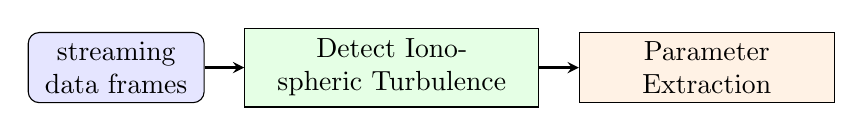
\begin{tikzpicture}[node distance=1.5cm, auto]

    \node (in) [startstop,text width=2cm] {streaming data frames \par};

    \node (detect) [compute, right of=in,text width=3.5cm,xshift=2cm] { Detect Ionospheric Turbulence \par };

    \node (reduce) [process, right of=detect, text width=3cm,xshift=2.5cm] { Parameter Extraction \par };


    \draw[arrow] (in) -- (detect);
    \draw[arrow] (detect) -- (reduce);

    \end{tikzpicture}

    \caption{Block diagram of general passive hitchhiker radar ionospheric turbulence detection algorithm.}
    \label{fig:fmgenalgo}
\end{figure} 
A more detailed view of the preliminary machine vision algorithm for each pixel is presented in Figure~\ref{fig:fmblock}.
\begin{figure}\centering 
    %the \par is necessary after each text to make the \baselineskip take effect
    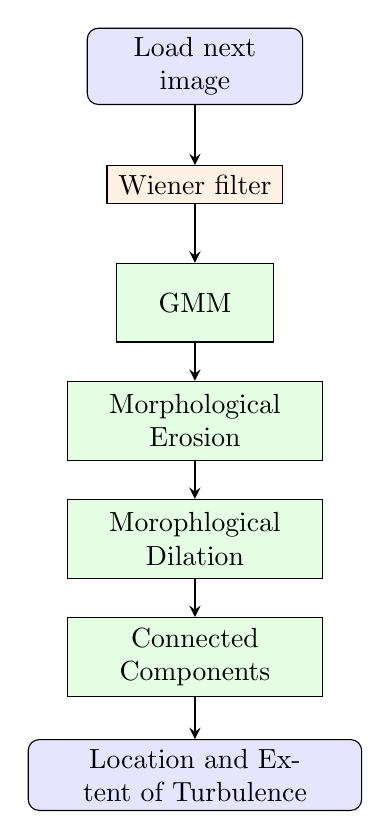
\begin{tikzpicture}[node distance=1.5cm, auto]
    
    \node (in) [startstop,text width=2.5cm] {Load next image};
    
    \node (filt) [process, below of=in,text width=2cm] { Wiener filter \par };
 
    \node (gmm) [compute, below of=filt,] { GMM \par };

	\node (erode) [compute, below of=gmm,text width=3cm] { Morphological Erosion \par};
    \node (dilate)[compute,below of=erode,text width=3cm] { Morophlogical Dilation \par};
    
    \node (conn) [compute,below of=dilate,text width=3cm] { Connected Components \par};
    
    \node (loc) [startstop,below of=conn,text width=4cm] { Location and Extent of Turbulence \par};
    
    \draw[arrow] (in) -- (filt);
    \draw[arrow] (filt) -- (gmm);
    \draw[arrow] (gmm) -- (erode);
    \draw[arrow] (erode) -- (dilate);
    \draw[arrow] (dilate) -- (conn);
    \draw[arrow] (conn) -- (loc);
    \end{tikzpicture}
    
    \caption{Passive hitchhiker radio computer vision algorithm for detecting ionospheric turbulence.}
    \label{fig:fmblock}
\end{figure}

Wiener filtering has been described in section~\ref{sec:filtnoise}.
After filtering, the dataframes pass to the main turbulence discrimination algorithm.

\subsection{Segmentation: Gaussian Mixture Method}

Originally reported by \citet{stauffer1999}, the Gaussian Mixture Method (GMM) is a dense algorithm used to distinguish to which of several Gaussian distributions the current pixel value belongs to.
For example, assume that background noise may be modeled with Gaussian pdf $N(\mu_1,\sigma_1)$, and that ionospheric turbulence follows Gaussian pdf $N(\mu_2,\sigma_2)$ and airplanes and meteors follow $N(\mu_3,\sigma_3), N(\mu_4,\sigma_4)$ and so on as illustrated in Figure~\ref{fig:gmm}.
\begin{figure}\centering
    \includegraphics[width=0.8\linewidth,trim=60 350 420 80,clip]{gfx/gmm}
    \caption{GMM examples of three distributions, where the output is the confidence of pixel value to each distribution.}\label{fig:gmm}
\end{figure}
Typically GMM implementations experience a few false positives, particularly for non-stationary noise, which are manifested as isolated pixels falsely declared as foreground.
Example GMM output using actual ISIS data is depicted in Figure~\ref{fig:gmmout}.
\begin{figure}\centering
    \includegraphics[width=\linewidth]{gfx/gmmout}
    \caption{GMM algorithm binary output (white desired) on actual ISIS range-Doppler dataframe}\label{fig:gmmout}
\end{figure}
The result clearly needs further processing; morphological algorithms are implemented.

\subsection{Morphological Erosion}
Morphological erosion is a set process in which a structuring element (SE), in this case a disk 3 pixels in diameter, is passed over each pixel in Figure~\ref{fig:gmmout}.
The erosion algorithm is described in section~\ref{sec:erode}.
For the data from Figure~\ref{fig:gmmout}, erosion results in Figure~\ref{fig:erodeout}.
\begin{figure}\centering
	\includegraphics[width=\linewidth,trim=0 20 0 20,clip]{gfx/erodeout}
	\caption{Erosion processed data with 3 pixel disk structuring element. Desired pixels in white. Turbulence has been isolated from clutter.}\label{fig:erodeout}
\end{figure}
The turbulence has been well-isolated from the clutter in Figure~\ref{fig:erodeout}.
However, the desired convex hull of pixels representing the actual ion-acoustic turbulence return have been eroded down to the point that connected components analysis will miss the associations of nearby pixels and declare a false negative--that no ionospheric turbulence existed here. 
The turbulence regions are reassociated by performing morphological dilation.

\subsection{Morphological Dilation}
Morphological dilation is a set process in which a structuring element is passed over pixel regions. 
Dilation is described in section~\ref{sec:dilate}.
For passive FM radar data, dilation is used to join associated regions of ionospheric turbulence in the processing of real passive radar data. 
The morphological dilation of actual data using a disk structuring element of diameter 5 pixels is shown in Figure~\ref{fig:dilateout}. 
\begin{figure}\centering
    \includegraphics[width=\linewidth,trim=0 20 0 20,clip]{gfx/dilateout}
    \caption{Dilation processed data with 5 pixel disk structuring element. Desired pixels in white. Artificial gaps have been filled in by dilation.}\label{fig:dilateout}
\end{figure}
After associated pixel regions of the ionospheric returns have been rejoined the dataframe is ready for connected component blob analysis.


\subsection{Connected Component Analysis}
To make a final declaration on ionospheric turbulence candidates, we consider whether a region of sufficient associated pixel extent in the range-Doppler space is observed. 
This will exclude events less than a user-defined space and Doppler extent. 
A future algorithmic extension would exploit the time dimension via Kalman filtering to better positively classify small-scale ionospheric turbulence. 
The connected component algorithm is described in section~\ref{sec:blob}.
Large self-ambiguity shifts occur for large changes in broadcast signal entropy--for example on a rock music station during DJ announcements or a brief quiet period during song transitions. 
An example CCA for real data is shown in Figure~\ref{fig:ccaout}.
\begin{figure}
    \includegraphics[width=\linewidth]{gfx/ccaout}
    \caption{CCA target detection inside green box. Color represents signal to clutter ratio.}
    \label{fig:ccaout}
\end{figure}
The green box neatly highlights the detected ionospheric turbulence. 
Parameters of the turbulence (Doppler centroid--average velocity and range) can be directly estimated from the CCA bounding box characteristics.

\subsection{Real data analysis}
Several data frames are shown in Figure~\ref{fig:gmmdump} as an example of performance on real-world data. 
The code \citet{cviono} was forwarded to the MIT Haystack research for implementation on existing ISIS data and for the RAPID system in testing.
Initial results have shown adequately low Type I and Type II errors, with further improvement possible by tracking behavior through space and time instead of time only.
\begin{figure}\centering
    \begin{subfigure}[t]{0.45\linewidth}
        \includegraphics[width=\linewidth]{gfx/out-000}	
        \caption{23:14:59 two turbulent regions detected.}
    \end{subfigure}
    \quad
    \begin{subfigure}[t]{0.45\linewidth}
        \includegraphics[width=\linewidth]{gfx/out-001}
        \caption{23:15:09 one turbulent region detected.}
    \end{subfigure}
    \begin{subfigure}[t]{0.45\linewidth}
        \includegraphics[width=\linewidth]{gfx/out-002}
        \caption{23:15:19 one large turbulent region detected.}
    \end{subfigure}
    \begin{subfigure}[t]{0.45\linewidth}
        \includegraphics[width=\linewidth]{gfx/out-003}
        \caption{23:15:29 two adjacent turbulent regions detected.}
    \end{subfigure}
\end{figure}
\begin{figure}\ContinuedFloat \centering
    \begin{subfigure}[t]{0.45\linewidth}
        \includegraphics[width=\linewidth]{gfx/out-004}
        \caption{23:15:39 one turbulent region detected.}
    \end{subfigure}
    \begin{subfigure}[t]{0.45\linewidth}
        \includegraphics[width=\linewidth]{gfx/out-005}
        \caption{23:15:49 two small turbulent regions detected.}
    \end{subfigure}
    \caption{Real data sequence from Aug 3, 2010. Ionospheric turbulence detections enclosed in green boxes.}
    \label{fig:gmmdump}
\end{figure}
\cleardoublepage
\chapter{DMC/HiST Systems Operations Guide}
\label{chapter:ops}
\thispagestyle{myheadings}

\graphicspath{{Ops/}}

\section{Summary}
The vision for the DMC and HiST system software and hardware was collaborative and one that would be reusable by its general nature.
By breaking the software and hardware build tasks up into incremental small parts, several engineering undergraduate and graduate students contributed meaningfully in a scaled-down version of the CubeSat teaming model. 
The DMC system is designed as a testbed for HiST multi-site operations, while DMC synchronizes multiple cameras at one site.
The cameras used for DMC were an Andor Neo and Andor iXon, as these were the cameras available at the time and low budget precluded purchasing purpose-obtained cameras.
The Andor Neo sensor coupled with the Marshall \unit[140]{mm} lens gave more resolution than necessary, so 4x4 or 8x8 binning was typically implemented (see section~\ref{sec:dmc} for details).
Cropping and binning the Neo sensor (reduced resolution) leads to a system where the Neo can be used to record all night and post-process (remove unwanted frames) with open-source software tools during the day. 


\section{Experimental Notes}
The DMC system was first controlled remotely on 2012 AUG 29. 
Both cameras were focused at nautical twilight the partly cloudy evening of 2012 AUG 30. 
The Kowa \unit[8.5]{mm} lens was resolving stars to single pixels on the iXon at the edges of the lens--the center focus is not as good. 
The Marshall/Neo focus was bad, and ultimately required removing the dome and replacing with flat glass due to near-field effects with the Marshall large aperture. 
A model of solar zenith angle was implemented to predict when useful observation times would occur, as seen in Figure~\ref{fig:solar2012}. 
\begin{sidewaysfigure}\centering
	\includegraphics[width=\textwidth]{gfx/Solar2012}
	\caption{Solar elevation at Søndrestrøm}\label{fig:solar2012}
\end{sidewaysfigure}
September through April will provide adequate viewing conditions at night, and the sun is not directly illuminating the sensor during the day.
The plate scaling occurs through \citet{hirschastro,lang2010} for each camera.

Observations on system operation with regard to slow network connection (as occurs due to Greenland Internet or anywhere with weak 3G/4G signal):
\begin{enumerate}
    \item Internet bandwidth is restricted--range of \unit[5]{kB/s} (1996 dialup modem speed) to \unit[60]{kB/s} (3G mobile connection). 
    \item GUI-based remote control is jumpy and sporadic 
    \item Image preview operation are quite slow and rapid progressions of image displays (i.e. video) cause loss of ability to control DMC PC.
    \item Downloads/uploads are dropped repeatedly if bigger than \unit[5]{MB}--files bigger than \unit[5]{MB} must be broken up into multiple segments
    \item lossy 200:1 compression needed to get even simple image previews 
    \item MATLAB campus license does not work due to inaccessible license server off-campus.
\end{enumerate}

Programming software and utilities available on DMC/HiST include: Labview 64-bit, Python 3.6, ImageMagick, Cygwin and Windows Subsystem for Linux.
At the project kickoff, it was decided to start with Labview control as Labview is known for robust multi-threaded control of unattended industrial equipment.
A simple program was written in Labview to start/stop acquisition based on a daily schedule oriented around when SZA$> 100^\circ$.
The Python asynchronous daemon waits for the Labview acquisition to stop, then begins automated computer vision processing of the day's data.
Windows Subsystem for Linux (WSL) is a Microsoft factory feature of Windows allowing access to a very large subset of Linux functionality at nearly the same performance as a bare-metal Linux install from within Windows.
WSL avoids the recompilation hassles and significant performance limitations of Cygwin.
WSL currently comes standard with Ubuntu 16.04 (the latest stable version), and other version of Linux can be installed within WSL as desired.

\section{Automatic Software Workflow}\label{sec:autoAlgo}
\texttt{cron} jobs act as backups to the main Python and Labview daemons, to help protect the cameras in case of an unexpected software failure.
The main Labview program is stored under \texttt{c:/code/lvsite}. 
The basic Labview user interface mirrors the variables stored in XML, so that external programs easily parse the experiment configuration for off-line data use.
Unlike standard Labview programs, the graphical interface is deemphasized because of the slow and intermittent Internet connectivity typical of remote systems.
Each day, four files are saved under folder \texttt{d:/YYYY-MM-DD/} that are automatically read by data post-processing programs.
\begin{table}\centering
    \caption{Files produced each night by the HiST recording software.}\label{tab:filewritten}
    \begin{tabular}{p{2cm}p{12cm}}
    \toprule
    file & description \\
    \midrule
    \texttt{.xml} & Human-readable header file detailing many camera parameters \\
    \texttt{.data} & If cameras had one or more trigger events, this file holds raw 16-bit unsigned grayscale data. May be up to about \unit[400]{GB} in size from a single nights recording, if the iXon recorded all night full-frame at \unit[33]{fps}. Ideally the iXon would trigger only a small portion of the night, recording \unit[17.5]{MB/s} of data \\
    \texttt{.log} & Copies the ``program status'' text box output from the GUI to a file, posts to Dropbox automatically each day\\
    \texttt{.synoptic} & Regardless of trigger status, system records a 16-bit grayscale frame to disk every $N$ Consumer Loop iterations. Typically $N=60$. \\
    \bottomrule
    \end{tabular}
\end{table}

\section{Experiment Design}\label{sec:ExpDes}
The field of view accessible via camera is strongly dependent on frame rate. 
Table~\ref{tab:camParamSpeed} lists a few of the relevant parameters. 
Figure~\ref{fig:ixonFOV} shows the iXon classic projected FOV with frame transfer. 
Figure~\ref{fig:neoFOV} shows the Neo projected FOV with 16-bit readout and global shutter.
Table~\ref{tab:compFPS} shows compatible frame rates between the Neo and iXon with these settings.

Note: FOVs of Figure~\ref{fig:overviewFOV} are notional only with 8.5mm Kowa lens on iXon and 140mm Marshall lens on Neo--actual FOV must be calculated using the desired lens.
\begin{table}\centering
\caption{Compatible frame rates for Neo (16-bit, global shutter) and iXon (14-bit, frame transfer)}
\label{tab:compFPS}
\begin{tabular}{ccc}
\toprule
Frames/sec & iXon (pixels, binning,exp.(ms)) & Neo (pixels,exp.(ms)) \\
\midrule
32.78 & 512 x 512, 1x1, 29.6 & 2560 x 1200, 20.0 \\
61 & 512 x 256, 1x1, 15.1 & 2560 x 600, 12.5 \\
75 & 512 x 206, 1x1, 12.4 & 2560 x 512, 10.5 \\
100 & 512 x 146, 1x1, 9.0 & 2560 x 384, 8.0 \\
\bottomrule
\end{tabular}

\end{table}

\begin{table}\centering
\caption{Camera parameters vs. frame rate effect}
\label{tab:camParamSpeed}
    \begin{tabular}{cccc}
        \toprule
        Camera & Binning & Width & Height\\
        \midrule
        Neo & No & No & Yes\\
        iXon & Yes & No & Yes\\
        \bottomrule
    \end{tabular}
\end{table}
\begin{figure}    \centering
    \includegraphics[trim=300 10 300 10,clip,width=\textwidth]{gfx/FOV}
    \caption{Relative FOV of Neo and iXon}\label{fig:overviewFOV}
\end{figure}
\begin{figure}    \centering
    \includegraphics[trim=2650 1050 20 950,clip,width=0.8\textwidth]{gfx/sensorsSize}
    \caption{Notional FOV of iXon with 8.5mm Kowa lens}\label{fig:ixonFOV}
\end{figure}
\begin{figure}  \centering
    \includegraphics[trim=30 450 1600 450,clip,width=\textwidth]{gfx/sensorsSize}
    \caption{Notional FOV of Neo with 8.5mm Kowa lens}\label{fig:neoFOV}
\end{figure}

\section{LabVIEW data acquisition algorithm}
The Labview algorithm consists of four loops executing in parallel, each with selectable priority. 
This ability is one of the two key reasons Labview was chosen for this project.
The other key reason is that all essential functionality was demonstrated from scratch in two weeks from a blank sheet. 

\subsection*{Producer}

This loop is particular to the camera or device in use--one loop per imaging device.

\begin{algorithm}
	\caption{Producer}
	\begin{algorithmic}
		\While{SZA $> 100^\circ$}
		\If{numberOfFramesInBuffer $> M$}
			\State  PCIe FPGA $\leftarrow$ $M$ frames $\leftarrow$ Camera FPGA 
			\State DMA: PC RAM Ring buffer $\leftarrow$ $M$ frames $\leftarrow$ PCIe FPGA
		\EndIf
		\EndWhile
	\end{algorithmic}
\end{algorithm}

\subsection*{Consumer}
This loop is generic--one loop per imaging device.

\begin{algorithm}
	\caption{Consumer}
	\begin{algorithmic}
		\Procedure{Long term storage}{}
		\While{SZA $> 100^\circ$}
		\State HDD $\leftarrow$ RAM Queue
		\EndWhile
		\EndProcedure

		\Procedure{Synoptic Recording}{}
		\While{SZA $> 100^\circ$}
			\If{more than $N$ seconds since last synoptic frame}
			\State HDD \texttt{.synoptic} file $\leftarrow$ average image of last ten frames in Queue
			\State Copy last frame of synoptic file to \texttt{.png} for web server ``live'' image
			\EndIf
		\EndWhile
		\EndProcedure
	\end{algorithmic}
\end{algorithm}

\subsection*{Network}
This loop handles orderly shutdown of the system from error or remote commands.
It uses TCP/IP sockets implemented as Labview Network Shared Variables to accomplish this.

The ``SanityCheck'' range of expected intensities $I$ is based on a 16-bit camera--adjust according to the relevant device.
Here, 100 is chosen as a number below the mean imaging chip noise based on typical camera gain settings.
For a narrow FOV camera with BG3 filtering, the image should never saturate with diffuse aurora. 
Saturation (low or high values) may be an indication of excess light reaching the imaging chip, therefore the system shuts down for the night, which closes the built-in camera shutter.
An example of a situation outside of system failure that might introduce excess light is a flashlight or laser shining into the camera--recall these cameras are deployed to unattended locations where anyone might walk by.

\begin{algorithm}
	\caption{Network}
	\begin{algorithmic}
		\Procedure{Failsafe}{}
		\While{SZA $> 100^\circ$}
		\State Poll TCP/IP socket values
		\If{NetworkShutdown \textbf{or} Error}
		\State Stop Producer and Consumer loops
		\EndIf
		\EndWhile
		\EndProcedure
		
		\Procedure{SanityCheck}{}
		\While{SZA $> 100^\circ$}
		\If{last three \texttt{.synoptic} $100 < \overline{I} < 60000 $ }
		\State Stop Producer and Consumer loops as saturation may be indication of excess light on imager chip
		\EndIf
		\EndWhile
		\EndProcedure
	\end{algorithmic}
\end{algorithm}

\subsection*{Schedule}
The schedule loop is the outermost loop, never closing except by operator command.
It starts and stops the recordings each day.
\begin{algorithm}
	\caption{Schedule}
	\begin{algorithmic}
		\Repeat
		\If{SZA $> 100^\circ$}
		\State Start Producer, Consumer, and Network loops
		\EndIf
		\If{SZA $< 100^\circ$}
		\State Stop Producer and Consumer loops
		\EndIf
		\Until{Operator Shutdown}
	\end{algorithmic}
\end{algorithm}

\section{Manual Software Workflow}\label{sec:ManWork}
This section covers diagnostic functions that are generalizable to auroral imaging systems.
The software that controls day-to-day recording should generally not have a graphical output for best overall system stability.
This allows the software to run without a graphical desktop at all, greatly enhanced operating system stability and security.
This principle greatly simplifies the recording software, further increasing robustness.
The camera is aimed and focused using the Andor Solis software, which also installs the camera SDK.
The operation of the system is automatically verified by basic sanity checks of the \texttt{.synoptic} file in the Network loop.


The operation of the system may be manually verified upon login to the Flask webserver on each site's PC.
This Flask server is not made available to the public to avoid DDOS-style attacks.
However, an external webserver may poll the cameras (with Flask configured to protect against excessive poll rates) and relay the latest pictures to the public.
This is implemented at the Søndrestrøm site.


The Python script used for detection of Alfvénic aurora is described in chapter~\ref{chapter:discrim}.
The Alfvénic aurora detection algorithm \citep{cviono} may be manually run by executing the command
\begin{verbatim}
python Detect.py ~/data/YYYY-MM-DD/*.DMCdata -p dmc.ini
\end{verbatim}
where \texttt{YYYY-MM-DD} is according to the data date of interest.

\subsection{Connecting to the DMC/HiST systems}
The systems are securely remotely controlled via SSH Public Key Authentication.
This means authorized users must have an encrypted file pair \textit{and} the corresponding password to access the system.
Each PC used to control the system remotely has a unique key, so that individual users can be deactivated if a problem occurs.
A simple script (saved to a text file) is executed to connect.
\begin{verbatim}
#!/bin/sh
ssh -f -p 22 -L 3391:4.3.2.1:3389 1.2.3.4 sleep 1;
xfreerdp /cert-ignore /v:localhost:3391
\end{verbatim}

 % include doesn't work
\end{appendices}
%==========================================================================%
% Bibliography
\nolinenumbers
\newpage
\singlespace
\raggedright % helps URLs and DOIs not blast into right margin so much.
\bibliographystyle{apalike-refs}

% each subdirectory can have its own BiBTeX file
\bibliography{thesis}
\cleardoublepage

%==========================================================================%
% Curriculum Vitae
% \include{Prelim/cv} 

%==========================================================================%
\end{document}
